%****************************************************
%	CHAPTER 4 - PIPELINE DESIGN
%****************************************************
\chapter{Pipeline Design}
\label{chap:systemDesign}

This chapter's objective is to detail the core design process of this project, a wave parameter extraction pipeline. The fundamental design which needed to be achieved was the extraction of wave parameters from \acs{sar} data. In order to achieve this, 

% \begin{figure}[H]
%     \centering
%     \resizebox{0.9\linewidth}{!}{
\definecolor{c1a1a1a}{RGB}{26,26,26}
\definecolor{c999999}{RGB}{153,153,153}
\definecolor{cff6600}{RGB}{255,102,0}
\definecolor{cb3b3b3}{RGB}{179,179,179}
\definecolor{navy}{RGB}{0,0,128}


\def \globalscale {1.000000}
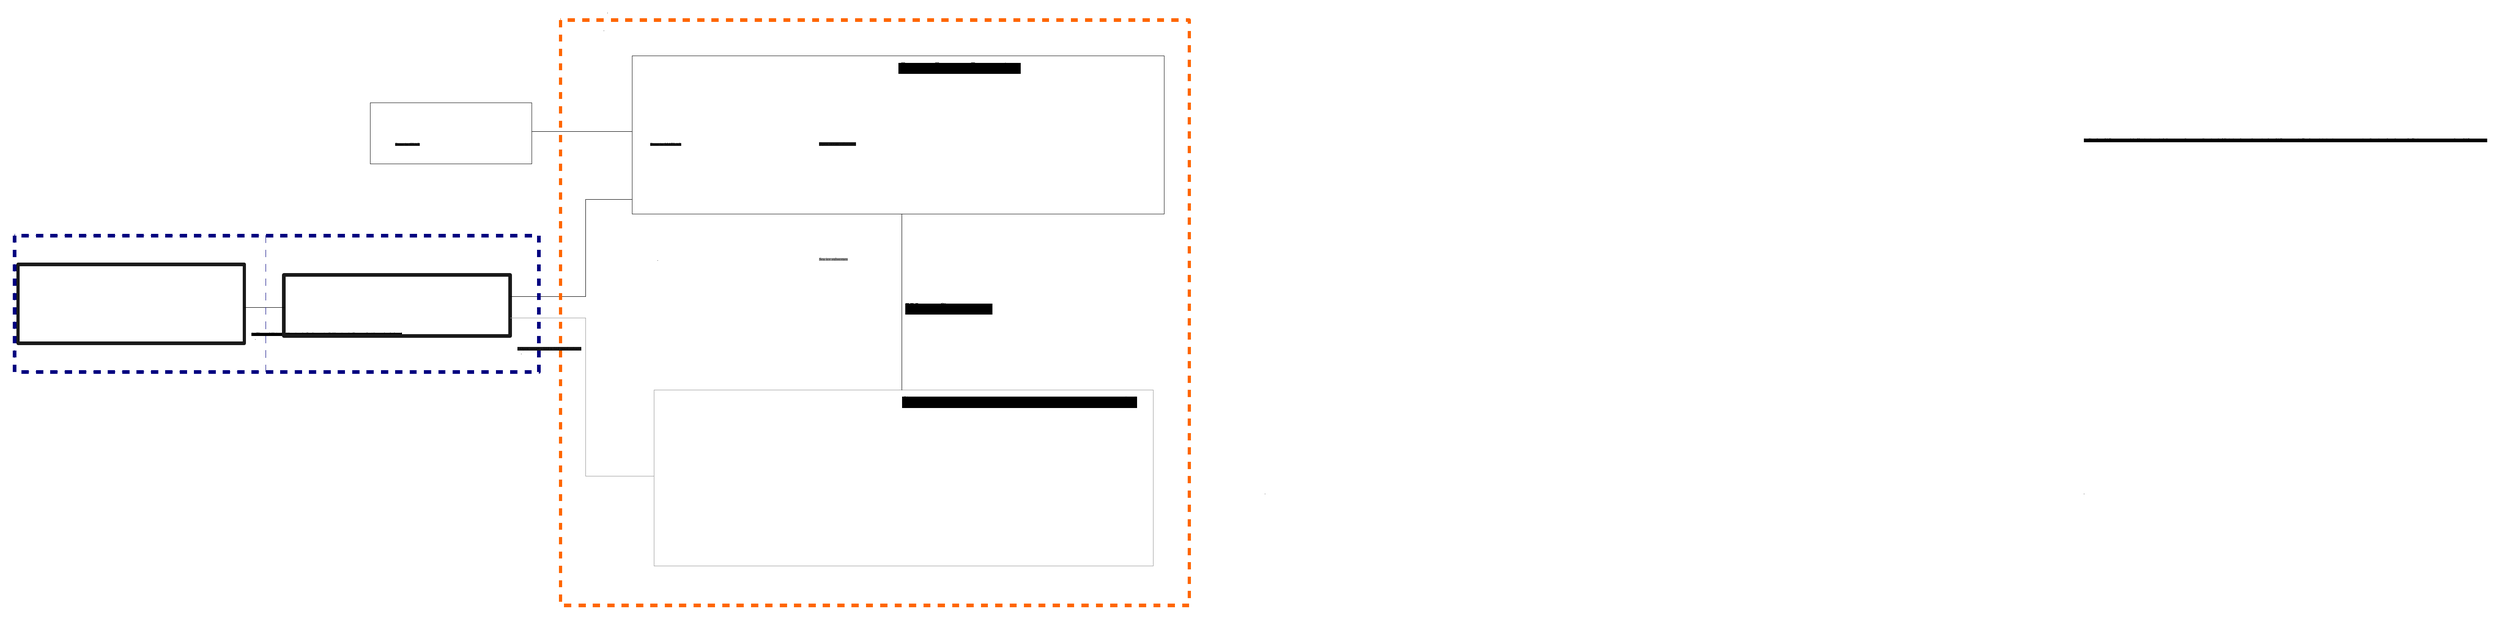
\begin{tikzpicture}[y=1cm, x=1cm, yscale=\globalscale,xscale=\globalscale, inner sep=0pt, outer sep=0pt]
  \path[draw=c1a1a1a,fill=c1a1a1a,fill opacity=0.0,line cap=butt,line
  join=round,line width=0.1cm] (0.2, 22.1) rectangle (6.5, 19.9);
  \node[fill=black,cm={ 0.3,-0.0,-0.0,0.3,(-2.0, 17.6)},anchor=south west]
  (text2) at (8.8, 2.4){};      \node[fill=black,cm={ 0.3,-0.0,-0.0,0.3,(-2.0,
  17.6)},anchor=south west] (text3) at (8.7, 2.5){1. Thermal Noise Calibration
  2. Radiometric Calibration  3. Extract Incidence Angle band};
  \path[draw=c1a1a1a,fill=blue,fill opacity=0.0,draw opacity=1.0,line
  cap=butt,line join=round,line width=0.1cm] (7.6, 21.8) rectangle (13.9, 20.1);
  \node[fill=black,cm={ 0.3,-0.0,-0.0,0.3,(5.4, 17.2)},anchor=south west]
  (text2-9) at (8.8, 2.4){};      \node[fill=c1a1a1a,cm={
  0.3,-0.0,-0.0,0.3,(5.4, 17.2)},anchor=south west] (text3-5) at (8.7, 2.5){-
  Open ocean  - 512 x 512 pixel subsets};      \path[draw=c1a1a1a,fill=blue,fill
  opacity=0.0,draw opacity=1.0,line cap=butt,line join=round,line width=0.0cm]
  (10.0, 26.6) rectangle (14.5, 24.9);      \node[fill=black,cm={
  0.3,-0.0,-0.0,0.3,(7.8, 22.0)},anchor=south west] (text2-9-0) at (8.8, 7.1){};
  \node[fill=c1a1a1a,cm={ 0.3,-0.0,-0.0,0.3,(7.8, 22.1)},anchor=south west]
  (text3-5-9) at (8.7, 6.5){};      \node[fill=c1a1a1a,cm={
  0.3,-0.0,-0.0,0.3,(13.8, 18.9)},anchor=south west] (text3-5-9-5-1) at (8.7,
  6.5){Open ocean subscenes};      \node[fill=c1a1a1a,cm={
  0.3,-0.0,-0.0,0.3,(9.3, 15.7)},anchor=south west] (text3-5-9-5-1-9) at (8.7,
  6.5){};      \node[fill=c1a1a1a,cm={ 0.3,-0.0,-0.0,0.3,(9.1,
  18.9)},anchor=south west] (text3-5-9-5-1-9-0) at (8.7, 6.5){Done in MATLAB};
  \node[fill=c1a1a1a,cm={ 0.3,-0.0,-0.0,0.3,(2.0, 18.9)},anchor=south west]
  (text3-5-9-5-1-9-0-5) at (8.7, 6.5){Done in SNAP};   \node[fill=c999999,cm={
  0.3,-0.0,-0.0,0.3,(13.8, 15.7)},anchor=south west]   (text3-5-9-5-1-2) at
  (8.7, 6.5){Sea ice subscenes};      \path[draw=black,even   odd rule,line
  cap=butt,line join=miter,line width=0.0cm] (6.5, 20.9) -- (7.6,   20.9);
  \path[draw=c1a1a1a,fill=blue,fill opacity=0.0,draw   opacity=1.0,line
  cap=butt,line join=round,line width=0.0cm] (17.3, 27.9)   rectangle (32.1,
  23.5);      \node[fill=black,line width=0.0cm,anchor=south   west] (text6) at
  (24.7, 27.4){Open Ocean Inversion};   \node[fill=black,cm={
  0.3,-0.0,-0.0,0.3,(-0.2, 20.3)},anchor=south west]   (text7) at (57.9, 5.2){1.
  Simulate SAR spectrum ( 2. Use in-situ wind data to   confirm wave direction
  3. Minimise observed vs. simulate SAR spectra  4.   Further minimisation w.r.t
  propogation direction of peak wave  5. Estimate   wave spectrum from SAR
  spectrum};      \path[draw=c999999,fill=blue,fill   opacity=0.0,draw
  opacity=1.0,line cap=butt,line join=round,line width=0.0cm]   (17.9, 18.6)
  rectangle (31.8, 13.7);      \node[fill=black,line   width=0.0cm,anchor=south
  west] (text6-9) at (24.8, 18.1){Sea Ice Inversion   Wave propogation model};
  \node[fill=black,cm={ 0.3,-0.0,-0.0,0.3,(-0.2,   10.5)},anchor=south west]
  (text7-6) at (57.9, 5.2){};   \path[draw=black,even odd rule,line
  cap=butt,line join=miter,line width=0.0cm]   (24.8, 23.5) -- (24.8, 18.6);
  \node[fill=black,line   width=0.0cm,anchor=south west] (text19) at (24.9,
  20.7){Wave Spectrum};   \path[draw=c999999,line cap=butt,line join=miter,line
  width=0.0cm] (13.9,   20.6) -- (14.9, 20.6) -- (16.0, 20.6) -- (16.0, 16.2) --
  (17.9, 16.2);   \path[draw=black,line cap=butt,line join=miter,line
  width=0.0cm] (13.9, 21.2)   -- (16.0, 21.2) -- (16.0, 23.9) -- (17.3, 23.9);
  \path[draw=cff6600,fill=cb3b3b3,fill opacity=0.0,draw opacity=1.0,line
  cap=butt,line join=round,line width=0.1cm,dash pattern=on 0.2cm off 0.2cm]
  (15.3, 28.9) rectangle (32.8, 12.6);      \path[draw=navy,fill=cb3b3b3,fill
  opacity=0.0,draw opacity=1.0,line cap=butt,line join=round,line
  width=0.1cm,dash pattern=on 0.2cm off 0.2cm] (0.1, 22.9) rectangle (14.7,
  19.1);      \path[draw=navy,fill=cb3b3b3,fill opacity=0.0,draw
  opacity=1.0,line cap=butt,line join=round,line width=0.0cm,dash pattern=on
  0.2cm off 0.2cm] (0.1, 22.9) rectangle (7.1, 19.1);   \node[fill=c1a1a1a,cm={
  0.3,-0.0,-0.0,0.3,(26.2, 9.2)},anchor=south west]   (text3-5-9-5-1-4) at (8.7,
  6.5){};      \path[draw=black,even odd rule,line   cap=butt,line
  join=miter,line width=0.0cm] (14.5, 25.8) -- (17.3, 25.8);
\end{tikzpicture}
}
%     \caption{Block Diagram in tex}
%     \label{fig:testPlotBlock}
% \end{figure}

% \begin{figure}[H]
%    \centering
%    %\begin{tabular}{@{}c@{\hspace{.2cm}}c@{}}
%        \includegraphics[page=1,width=.9\linewidth]{Figures/PipelineDesign/overall_project.pdf}
%    %\end{tabular}
%  \caption{Test}
%  \label{fig:Test}
% \end{figure}


This chapter begins by providing an overview of the entire pipeline - part of which falls outside of the scope of this project, however, this context is relevant in terms of giving context to the desired results for this project in the context of the broader goals of this pipeline. Each subsequent section will unpack the five main sub-modules within the pipeline in a respective section. Each of these sections will further break down the sub-module into smaller blocks which make up the sub-module. The use of block diagrams allows the process the be understood in terms of the flow of the pipeline, and block diagrams are used throughout this chapter to break down higher-level processes. The variable and function names utilised in this chapter, match those used in the \textsc{Matlab} pipeline.

\section{Overview} \label{sec:systemDesign.overview}

As detailed in xxx, this project required wave parameter extraction for use in a sea ice parameter extraction pipeline. This entire system design is shown as a block diagram in Figure \ref{fig:systemDesign.wholeProject}. It is evident from Figure \ref{fig:systemDesign.wholeProject}, which parts of the \acs{sar} sea ice parameter are relevant to this project. A more detailed block diagram of the wave parameter extraction process is shown in Figure \ref{fig:systemDesign.scope} and within this pipeline, five main functional blocks were identified and are highlighted by five unique colours. [ADD WAVE SPECTRUM GENERATION PIECES] [MENTION USE OF STRUCTURES THROUGHT]
% Will still change
\begin{figure}[H]
    \centering
    \includegraphics[width=.95\linewidth]{Figures/PipelineDesign/overall_project.pdf}
    \caption{Pipeline system design in the context of the entire parameter extraction process. The scope of this project is shown in black text, with parts of the pipeline outside of the scope, shown in grey.}
    \label{fig:systemDesign.wholeProject}
\end{figure}

% Word better and slim down - ADD DISCUSSION ON WAVE SPECTRUM GENERATION
The five functional blocks were identified as \textsc{pre-processing}, \textsc{metadata extraction}, \textsc{\acs{sar} spectrum calculation}, \textsc{wave spectrum generation}, and \textsc{inversion}. The \textsc{pre-processing} block involves the use of the \ac{snap} Toolbox developed by \ac{esa} as well as \textsc{Matlab}, developed by MathWorks Inc. The \textsc{pre-processing} block reads in a downloaded \acs{sar} Level-1 \ac{grd} data file and outputs a \textsc{Matlab} structure array\footnote{In \textsc{Matlab}, a structure array is a type of data that organises related data into groups. These groups are indexed using an associated field value which can hold any particular data type. More information on structure arrays can be found in the \href{https://www.mathworks.com/help/matlab/ref/struct.html}{\textsc{Matlab} documentation}. The rest of this report will refer to structure arrays simply as structures.} of \lstinline[columns=fixed]{n} equal-sized transects. These equal-sized transects can be input to the \textsc{inversion} block. The output \ac{netcdf} file from \acs{snap} is used to generate views of \acs{sar} data in \textsc{Matlab}, as well as storing the metadata for the \textsc{metadata extraction} block. The \ac{netcdf} file is read by the \textsc{metadata extraction} block and outputs the desired metadata values required for the \textsc{\acs{sar} spectrum calculation} block. The \textsc{\acs{sar} spectrum calculation} block reads in a wave spectrum sourced from \ac{ncep} and generates a \acs{sar} spectrum of the provided wave spectrum. This generated \acs{sar} spectrum is input to the \textsc{inversion} block along with the output of the \textsc{metadata extraction} block. The \textsc{inversion} block outputs the wave parameters from the input pre-processed \acs{sar} data.
% Will still change
\begin{figure}[H]
    \centering
    \includegraphics[width=.95\linewidth]{Figures/PipelineDesign/4022_pipeline.pdf}
    \caption{Pipeline system design for the scope of this project broken down further than the entire pipeline shown in Figure \ref{fig:systemDesign.wholeProject}. All the required metadata and external models are shown, along with the part of the process that they are required.}
    \label{fig:systemDesign.scope}
\end{figure}
%====================================================
% PRE-PROCESSING
%====================================================
\section{Pre-processing} \label{sec:systemDesign.preProcessing}


\subsection{Overview} \label{subsec:systemDesign.preProcessing.Overview}

The pre-processing block of the pipeline was designed in a hybrid manner, with part of the pre-processing done in the \ac{snap} toolbox developed by \ac{esa} prior to the use of \textsc{Matlab} tools. The pre-processing block was designed to have an overall function of reading in \ac{s1a} data, apply the desired pre-processing techniques to the \acs{sar} data, and take 512x512 pixel sized transects of this larger \acs{sar} data. The applied pre-processing techniques to calibrate \acs{sar} data for wave parameter extraction were on the recommendation of Giacomo De Carolis and Francesca De Santi of the \acs{irea}, however, discussion around the use of different processing techniques is presented in Chapter \ref{chap:discussion}. The design of this block was designed to keep pre-processing outside of the \textsc{Matlab} environment to a minimum, through the use of external tools. 

The pre-processing block had six notable stages: Thermal noise calibration of \acs{s1a} \acs{grd} data, radiometric calibration of these data, extraction of individual pixel incidence angle, exporting calibrated \acs{grd} data to a usable format for \textsc{Matlab}, reading in the exported data, and taking 512x512 pixel transects of the larger \acs{sar} data. The flow of this block of the pipeline is shown graphically in Figure \ref{fig:systemDesign.preProcessing.blockDiagram}.

\begin{figure}[H]
    \centering
    \includegraphics[width=.95\linewidth]{Figures/PipelineDesign/pre_processing.pdf}
    \caption{Block diagram depicting an expanded pre-processing sub-block of Figure \ref{fig:systemDesign.scope}}
    \label{fig:systemDesign.preProcessing.blockDiagram}
\end{figure}

\subsection{Thermal Noise Calibration} \label{subsec:systemDesign.preProcessing.thermalNoise}

After obtaining \acs{grd} \acs{sar} data from \href{scihub.copernicus.eu/dhus/#/home}{Copernicus SciHub}, the first sub-block of the pre-processing block was Thermal Noise Calibration. \acs{s1a} data contains large amounts of thermal noise and as such, \acs{snap} contains a built-in function called \lstinline{S-1 Thermal Noise Removal}. For this block, this function was implemented in \acs{snap} Desktop and is detailed in \href{https://github.com/JNSRYA006/sar-parameter-extraction-pipeline/blob/main/functions/[pipeline.mlx]}{\lstinline{pipeline.mlx}}.

\subsection{Radiometric Calibration} \label{subsec:systemDesign.preProcessing.radiometric}

After removing thermal noise from \acs{grd} \acs{sar} data, the second sub-block of the pre-processing block was Radiometric Calibration. \acs{snap} contains a built-in function called \lstinline{Calibrate} within the \lstinline{Radiometric} block of functions. For this block, this function was implemented in \acs{snap} Desktop and is detailed in \href{https://github.com/JNSRYA006/sar-parameter-extraction-pipeline/blob/main/functions/[pipeline.mlx]}{\lstinline{pipeline.mlx}}.

\subsection{Incidence Angle Extraction} \label{subsec:systemDesign.preProcessing.incidenceAngle}

Due to the fact that the incidence angle varies for each pixel in \acs{sar} data, this exact per-pixel incidence angle is required in order to calculate Equations \ref{eq:hh.rar.Tt_k}, \ref{eq:hh.motion.Tv_k}, which form part of the co and autocovariance functions described in Section \ref{subsec:theory.hasselmann.sarImaging}. In order to achieve this, multiple approaches were investigated. 

Firstly, the metadata file from \acs{s1a} \acs{grd} data was found to contain near and far-look incidence angles. The initial idea to extract individual pixel incidence angle values was to use \textsc{Matlab}'s built-in \lstinline{linspace} function which creates an evenly spaced vector over the range of values. This was an incorrect implementation as the incidence angle is not a linear relation to the latitude and longitude of an image. Furthermore, this method meant that each longitude of the image contained the same incidence angle value, and only the latitude of the image changed.

Secondly, a second type of metadata from \acs{s1a} \acs{grd} data was investigated. This metadata was in the form of a tie-point grid, which provided a 4x4 matrix of incidence angle data, using \lstinline{linspace} on this metadata resulted in a per-pixel incidence angle value which changed in latitude, as well as longitude which is an improvement from the first method.

Finally, tie-point grid data was exported as a band using \acs{snap} Desktop. The way in which this is achieved is detailed in \href{https://github.com/JNSRYA006/sar-parameter-extraction-pipeline/blob/main/functions/[pipeline.mlx]}{\lstinline{pipeline.mlx}}. These data provide a pixel-by-pixel value of the incidence angle on the \acs{s1a} data. Exporting the tie-point grid as a band, allows this band to be imported in \textsc{Matlab} using the \lstinline{ncread} function discussed in Section \ref{subsec:systemDesign.preProcessing.importData}.

In order to decide which method to use, plots of these data were generated over a range of pixel values. Figure \ref{fig:systemDesign.preProcessing.incidence}.

\begin{figure}[H]
    \centering
    \begin{subfigure}{0.48\linewidth}
        \centering
        \resizebox{\linewidth}{!}{\input{Figures/PipelineDesign/4_tiePoint_incidence}}
        \caption{Second implemented method to obtain incidence angle. 4x4 tie-point grid.}
        \label{fig:systemDesign.preProcessing.incidence.4_tie}
    \end{subfigure}   
    \begin{subfigure}{0.48\linewidth}
        \centering    
        \resizebox{\linewidth}{!}{\input{Figures/PipelineDesign/linspcae_incidence}}
        \caption{Second implemented method to obtain incidence angle. \lstinline{linspace} of 4x4 tie-point grid.}
        \label{fig:systemDesign.preProcessing.incidence.4_tie.linspace}        
    \end{subfigure}
    \subcaptionbox{Third implemented method to obtain incidence angle. Exported band of incidence angle tie-point grid.\label{fig:systemDesign.preProcessing.incidence.pixel_tie}}[0.48\linewidth]{
        \resizebox{\linewidth}{!}{\input{Figures/PipelineDesign/pixel_tiePoint_incidence}}
    }
        \subcaptionbox{Difference between Figures \ref{fig:systemDesign.preProcessing.incidence.4_tie.linspace} and \ref{fig:systemDesign.preProcessing.incidence.pixel_tie}.\label{fig:systemDesign.preProcessing.incidence.difference}}[0.48\linewidth]{
        \resizebox{\linewidth}{!}{\input{Figures/PipelineDesign/difference_incidence}}
    }   
    \caption{Comparison of incidence angle data from 28-Jul-2023 at 34.78S, 16.77E. The second two methods discussed in Section \ref{subsec:systemDesign.preProcessing.incidenceAngle} are shown visually as a coloured image corresponding to associated incidence angle values, as indicated in the respective colour bars.}
    \label{fig:systemDesign.preProcessing.incidence}
\end{figure}

% Disucssion of plots (Look in ClickUp)


\subsection{\acs{netcdf} Export} \label{subsec:systemDesign.preProcessing.exportNetCDF}
% Discuss why netcdf
\acs{snap} Desktop allows a multitude of export options for pre-processed data. The choice of export data type was narrowed down to data formats which contained metadata, as well as the \acs{sar} data. A list of these formats is shown below.

\begin{itemize}
    \item GeoTIFF
    \item BEAM-DIMAP
    \item \ac{envi}
    \item \ac{hdf}5
    \item \ac{netcdf}4
\end{itemize}

In order to decide which file format to export data as from \acs{snap} Desktop, an analysis of the compatibility of each file format with \textsc{Matlab} was done and the following was found.

A GeoTIFF file can be read into \textsc{Matlab} using the \lstinline{readgeoraster} function built into the Mapping Toolbox provided by \textsc{Matlab}. BEAM-DIMAP is a file format used by \acs{snap} products, and cannot be imported to \textsc{Matlab}. An \ac{envi} file can be read into \textsc{Matlab} to extract metadata using the \lstinline{enviinfo} function built into the Image Processing Toolbox by \textsc{Matlab}. A \acs{hdf}5 file can be displayed and read in \textsc{Matlab} using a variety of functions built into \textsc{Matlab} such as the \lstinline{h5disp} and \lstinline{h5read} functions. Finally, a \acs{netcdf}4 file can, as with \acs{hdf}5 files, be displayed and read in \textsc{Matlab} using a variety of functions built into \textsc{Matlab}.

Of the 5 export file types, only BEAM-DIMAP cannot be read into \textsc{Matlab}. Due to the desire to only use built-in \textsc{Matlab} functions and not make use of external toolboxes, this left \acs{hdf}5 and \acs{netcdf}4 as the two file types to be chosen from. Both file formats are able to be loaded as a structure in \textsc{Matlab}, and as such are both desirable choices. However, exporting \acs{sar} data from \acs{snap} was faster when exporting as \acs{netcdf} as opposed to \acs{hdf}. Furthermore, \acs{ncep} data was downloaded as a \acs{netcdf} file, and in order to keep consistency, \acs{netcdf} was chosen as the file type to export from \acs{snap} Desktop.

\subsection{Matlab Data Import} \label{subsec:systemDesign.preProcessing.importData}

The first sub-block in the \textsc{Matlab} implementation of the pre-processing block was called \lstinline{ncread}. As discussed in Section \ref{subsec:systemDesign.preProcessing.exportNetCDF}, the \acs{netcdf} file format was used for all imported data into \textsc{Matlab}. The \href{https://www.mathworks.com/help/Matlab/ref/ncread.html}{\lstinline{ncread}} \textsc{Matlab} function was used to import the exported data from \acs{snap} Desktop.

In order to access different bands within the \acs{netcdf} file, different variable names were used as a second input parameter to the \href{https://www.mathworks.com/help/Matlab/ref/ncread.html}{\lstinline{ncread}} functions. Listing \ref{code:netCDFImport} details the required variable names to extract the two bands of interest required for each subsequent block, and sub-block in Figure \ref{fig:systemDesign.scope}.

\begin{lstlisting}[caption={\textsc{Matlab} code used to import all desired bands from exported \acs{netcdf} data from \acs{snap} Desktop.},label={code:netCDFImport}]
filepath = "D:\UCT\EEE4022S\Data\CPT\export_data.nc";
VV = ncread(filepath,'Sigma0_VV'); % Intensity VV pre-processed data
th = ncread(filepath,'Incidence_Angle'); % Incidence Angle band
\end{lstlisting}

By utilising \href{https://www.mathworks.com/help/Matlab/ref/ncread.html}{\lstinline{ncread}} to extract data, this assigns both \lstinline{VV} and \lstinline{th} variables to a nxm sized matrix, where n and m respectively represent the size of the \acs{sar} data in terms of cross-range and range directions. The extraction of metadata is detailed in Section \ref{subsec:systemDesign.metadata.import}.



\subsection{Take Transects and Subdivide Data} \label{subsec:systemDesign.preProcessing.transects}

The most important part of the pre-processing for wave parameter extraction for use in sea ice parameter extraction is the ability to 'follow' the flow of ocean waves into the \acs{miz}. To achieve this, transects of a fixed size are taken of open ocean scenes as well as sea ice scenes. This allows the way in which ocean waves propagate through sea ice to be studied, and due to this, sea ice parameters are able to be extracted using the models described in Section \ref{subsec:litReview.sarCharac.seaIceWaveModelling}. As per \cite{Wadhams2004,DeSanti2018} the size of these transects should be 512x512 pixels in size. Taking transects of a larger image in \textsc{Matlab} is relatively straightforward, however, these transects need to be able to be taken at an angle to follow the direction of the visible ocean waves. If the ocean wave direction is not followed, this could cause issues in determining the way in which ocean waves are attenuated in the \acs{miz}. Along with this, the transect needs to start at a certain location of the whole scene. Due to the fact that latitude and longitude are not encoded in the \acs{s1a} \ac{grd} data, it was decided that a pixel starting position would be used to determine the starting position.

Due to the way in which \textsc{Matlab} indexes arrays, which is counter-intuitive to other programming languages, with the initial index being given a value of \textsc{1}, a check that the start location of the first transect was a valid index in the imported sarData needed to be conducted. This was achieved using a simple \lstinline{if} statement. The way in which angled transects were designed to be taken is visually represented in Figure \ref{fig:systemDesign.transects}. 


\begin{figure}[H]
    \centering
    \includegraphics[width=.65\linewidth]{Figures/PipelineDesign/transects_w_SAR.pdf}
    \caption{Implemented geometry for taking transects of full \acs{sar} scene.}
    \label{fig:systemDesign.transects}
\end{figure}

$\theta$, in Figure \ref{fig:systemDesign.transects}, represents the user-supplied angle at which to take the $n$ number of 512x512 transects measured clockwise from the +$x$-axis. $x_{1},y_{1}$ represent the user-supplied pixel starting location at which transects should be taken from. The \href{https://github.com/JNSRYA006/sar-parameter-extraction-pipeline/blob/main/functions/preprocess/get512Transects.m}{\lstinline{get512Transects}} function was designed to incorporate all of these design decisions, and as a result, takes in the full scene of \acs{sar} data, the top left $x$ and $y$ coordinates, as well as the user-defined angle, $\theta$ and number of transects, $n$. \href{https://github.com/JNSRYA006/sar-parameter-extraction-pipeline/blob/main/functions/preprocess/get512Transects.m}{\lstinline{get512Transects}} returns a 512x512x$n$ array of the transects of the full scene, along with a $n$x4 matrix of the corner pixel values of each transect. As well as using the \href{https://github.com/JNSRYA006/sar-parameter-extraction-pipeline/blob/main/functions/preprocess/get512Transects.m}{\lstinline{get512Transects}} function to take transects of the \acs{sar} image, the function can also be used to take transects of the \lstinline{th} variable determined in Listing \ref{code:netCDFImport}. The returned variable for \lstinline{th} follows the same form as discussed above for \acs{sar} data.

In order to annotate the transects, the \href{https://github.com/JNSRYA006/sar-parameter-extraction-pipeline/blob/main/functions/preprocess/annotate512Transects.m}{\lstinline{annotate512Transects}} function was designed which allowed the user to control the colour of the transect outline, as well as text colour and need for a background on the text colour. Using both the \href{https://github.com/JNSRYA006/sar-parameter-extraction-pipeline/blob/main/functions/preprocess/get512Transects.m}{\lstinline{get512Transects}} and \href{https://github.com/JNSRYA006/sar-parameter-extraction-pipeline/blob/main/functions/preprocess/annotate512Transects.m}{\lstinline{annotate512Transects}} functions allowed the plots in Figure \ref{fig:systemDesign.transectSample} to be generated. The ability to view individual transects is desired to be able to follow the direction of waves within the \acs{sar} scene.

\begin{figure}[H]
    \centering
    \begin{subfigure}{0.65\linewidth}
        \centering
        \includegraphics[width=\linewidth]{Figures/PipelineDesign/VVSceneWTransects.pdf}
        \caption{Full \acs{s1a} VV scene.}
        \label{fig:systemDesign.transectSample.full}
    \end{subfigure}   
    \begin{subfigure}{0.95\linewidth}
        \centering    
        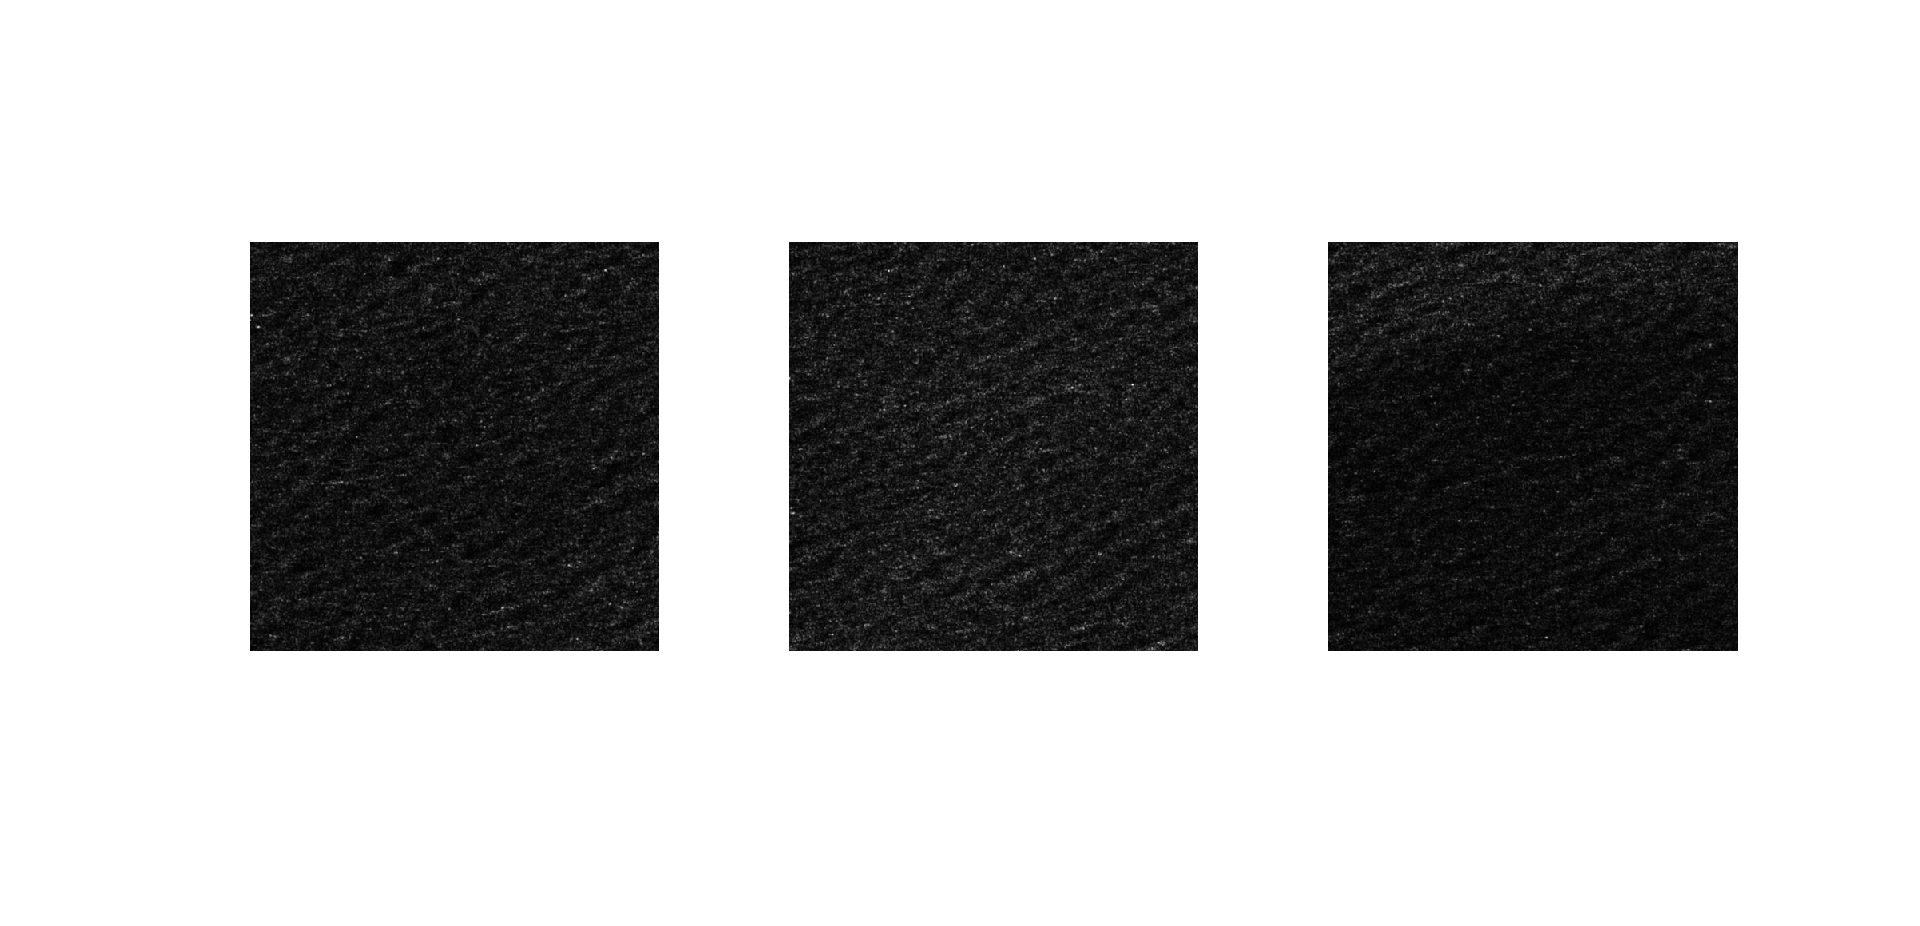
\includegraphics[width=\linewidth]{Figures/PipelineDesign/VVAllTransects.pdf}
        \caption{Transects 1 through 3 of Figure \ref{fig:systemDesign.transectSample.full} taken at 30$\degree$.}
        \label{fig:systemDesign.transectSample.all}        
    \end{subfigure}
    \caption{\acs{s1a} Intensity VV data, pre-processed according to Section \ref{sec:systemDesign.preProcessing}, from 28-Jul-2023 at 34.78\,S, 16.77\,E with transects at 30$\degree$ for $x_{1},y_{1} = 1,1$ displayed and labelled. Respective individual transects are shown.}
    \label{fig:systemDesign.transectSample}
\end{figure}
% Including geometry
% \begin{figure}[H]
%     \centering
%     \begin{subfigure}{0.48\linewidth}
%         \centering
%         \includegraphics[width=\linewidth]{Figures/PipelineDesign/VVSceneWTransects.pdf}
%         \caption{Full \acs{s1a} VV scene.}
%         \label{fig:systemDesign.transectSample.full}
%     \end{subfigure}   
%     \begin{subfigure}{0.48\linewidth}
%         \centering
%         \includegraphics[width=\linewidth]{Figures/PipelineDesign/transects_w_SAR.pdf}
%         \caption{Full \acs{s1a} VV scene.}
%         \label{fig:systemDesign.transectSample.full}
%     \end{subfigure}    
%     \begin{subfigure}{0.95\linewidth}
%         \centering    
%         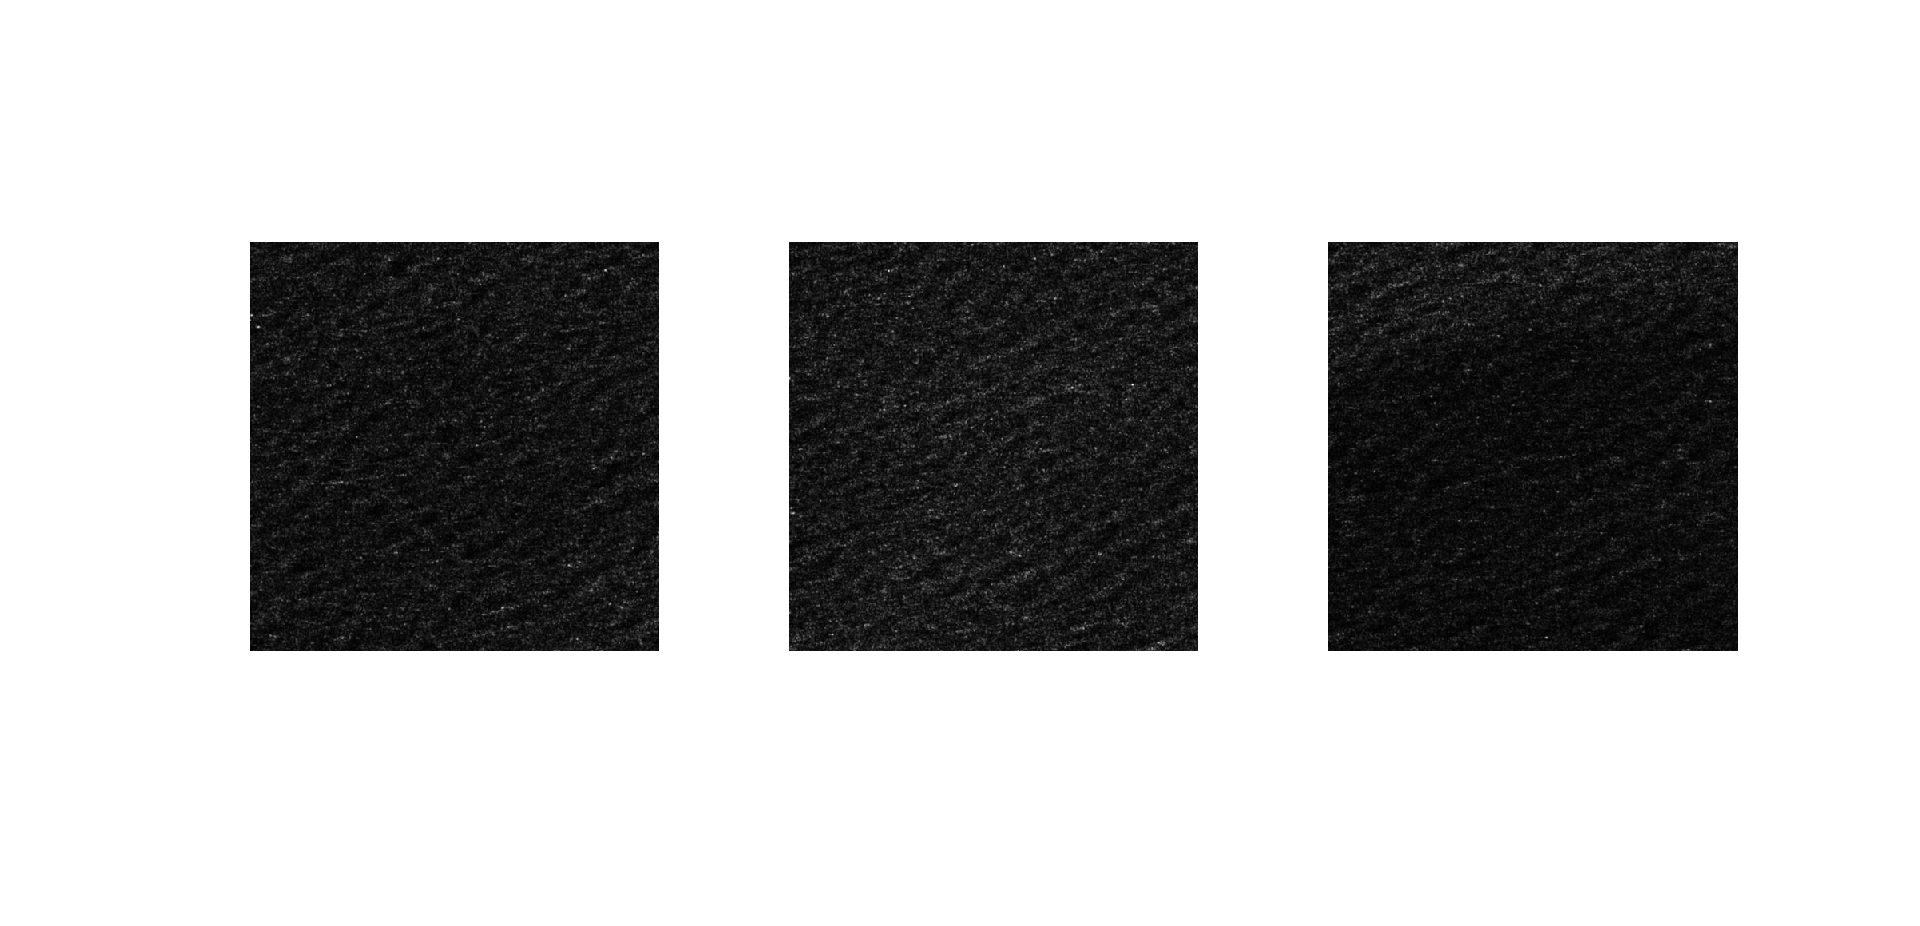
\includegraphics[width=\linewidth]{Figures/PipelineDesign/VVAllTransects.pdf}
%         \caption{Transects 1 through 3 of Figure \ref{fig:systemDesign.transectSample.full} taken at 30$\degree$.}
%         \label{fig:systemDesign.transectSample.all}        
%     \end{subfigure}
%     \caption{\acs{s1a} Intensity VV data, pre-processed according to Section \ref{sec:systemDesign.preProcessing}, from 28-Jul-2023 at 34.78\,S, 16.77\,E with transects at 30$\degree$ for $x_{1},y_{1} = 1,1$ displayed and labelled. Respective individual transects are shown.}
%     \label{fig:systemDesign.transectSample}
% \end{figure}

%====================================================
% METADATA EXTRACTION
%====================================================
\section{Metadata Extraction} \label{sec:systemDesign.metadata}

\subsection{Overview} \label{subsec:systemDesign.metadata.overview}

\begin{figure}[H]
    \centering
    \includegraphics[width=.85\linewidth]{Figures/PipelineDesign/metadataExtraction.pdf}
    \caption{Block diagram depicting an expanded metadata extraction sub-block of Figure \ref{fig:systemDesign.scope}}
    \label{fig:systemDesign.metadata.blockDiagram}
\end{figure}

\subsection{Data Import} \label{subsec:systemDesign.metadata.import}

The first sub-block of the metadata extraction block was called \lstinline{ncinfo}. As discussed in Section \ref{subsec:systemDesign.preProcessing.exportNetCDF}, the \acs{netcdf} file format was used for importing data into \textsc{Matlab}. The \href{https://www.mathworks.com/help/Matlab/ref/ncinfo.html}{\lstinline{ncinfo}} \textsc{Matlab} function was used to import the exported data from \acs{snap} Desktop.

In order to access the exported metadata within the \acs{netcdf} file the \href{https://www.mathworks.com/help/Matlab/ref/ncinfo.html}{\lstinline{ncinfo}} \textsc{Matlab} function was used. Listing \ref{code:netCDFImport} details the required variable name to extract the metadata for the subsequent sub-block in Figure \ref{fig:systemDesign.metadata.blockDiagram}.

\begin{lstlisting}[caption={\textsc{Matlab} code used to import metadata from exported \acs{netcdf} data from \acs{snap} Desktop.},label={code:netCDFImport.metadata}]
filepath = "D:\UCT\EEE4022S\Data\CPT\export_data.nc";
metadata = ncinfo(filepath,'metadata'); % Extract all metadata
\end{lstlisting}

Using \href{https://www.mathworks.com/help/Matlab/ref/ncinfo.html}{\lstinline{ncinfo}} to extract metadata, assigns the \lstinline{metadata} variable to a $1$x$1$ structure with all desired metadata in the \texttt{Attributes} field which can be parsed to the \href{https://github.com/JNSRYA006/sar-parameter-extraction-pipeline/blob/main/functions/preprocess/annotate512Transects.m}{\lstinline{filterAttributesNetCDF}} sub-block.


\subsection{Filter Attributes} \label{subsec:systemDesign.metadata.filter}

The \href{https://github.com/JNSRYA006/sar-parameter-extraction-pipeline/blob/main/functions/preprocess/annotate512Transects.m}{\lstinline{filterAttributesNetCDF}} block takes in a structure containing metadata, as well as a list of strings of the desired attributes to keep from all metadata values. Exact attribute names can be found in Table \ref{tab:ap.metadataVals} in Appendix \ref{ap:metadata}. The function outputs a \texttt{1xlength(reqAttributes)} structure with two columns: \texttt{Name} and \texttt{Value}. Additional metadata formatting functions are discussed in Section \ref{sec:systemDesign.sarSpectrum} and \ref{sec:systemDesign.inversion} when required by respective \acp{mtf}.

%====================================================
% WAVE SPECTRUM GENERATION
%====================================================
\section{Wave Spectrum Generation} \label{sec:systemDesign.waveSpectrum}



\subsection{Overview} \label{subsec:systemDesign.waveSpectrum.Overview}

\begin{figure}[H]
    \centering
    \includegraphics[width=.95\linewidth]{Figures/PipelineDesign/wave_spectrum.pdf}
    \caption{Block diagram depicting an expanded wave spectrum generation sub-block of Figure \ref{fig:systemDesign.scope}.}
    \label{fig:systemDesign.wavesSpectrum.blockDiagram}
\end{figure}

\subsection{Wave Data Download} \label{subsec:systemDesign.waveSpectrum.download}

\acs{ncep} \acs{noaa} wave data is available in 6-hour intervals. These intervals are 00, 06, 12, and 18 hours in UTC time. As \acs{s1a} captures are not set to exact time intervals, a function \href{https://github.com/JNSRYA006/sar-parameter-extraction-pipeline/blob/main/functions/waveSpectra/generateSingleJONSWAP.m}{\lstinline{getNOAAParams}} was created which took in the \acs{s1a} capture datetime object, obtained using the \href{https://github.com/JNSRYA006/sar-parameter-extraction-pipeline/blob/main/functions/waveSpectra/generateSingleJONSWAP.m}{\lstinline{getCaptureData}} function, and outputted two strings. Both of these strings were formatted as per the \acs{url} used to download \acs{ncep} wave data. 

The way in which the closest hour value was determined was using the code extract from \href{https://github.com/JNSRYA006/sar-parameter-extraction-pipeline/blob/main/functions/waveSpectra/generateSingleJONSWAP.m}{\lstinline{getNOAAParams}} shown in Listing \ref{code:waveSpec.download.closestHour}. 

\begin{lstlisting}[caption={Initial implementation of \textsc{Matlab} code to extract wave parameters at certain geographical location.},label={code:waveSpec.download.closestHour}]
noaaHour = datetime(SARCaptureDate,"Format","HH:mm");
noaaHour = double(hour(noaaHour));
allowedHours = [0,6,12,18];
hourDiff = abs(allowedHours - noaaHour);
[~,hourIndex] = min(hourDiff);
nearestHour = allowedHours(hourIndex);
\end{lstlisting}

The date of the \acs{s1a} capture was extracted using \textsc{Matlab}'s built-in \lstinline{datetime} function. The form of the date and hour value required by \acs{ncep} was of the form \texttt{YYYYMMDD} and \texttt{HH} respectively. To achieve this, the \href{https://github.com/JNSRYA006/sar-parameter-extraction-pipeline/blob/main/functions/waveSpectra/generateSingleJONSWAP.m}{\lstinline{getNOAAParams}} used basic string handling after extracting all individual values. Interestingly, isolating a month or day from a datetime object with a numeric value $<$ 10 in \textsc{Matlab}, resulted in a single character. As \acs{ncep} required two characters for both of these parameters, a simple \lstinline{if} statement checked the length of the value, and updated them accordingly if they had length 1 by prepending a \texttt{0} to the front of the single character value.

These functions allowed associated wave data to be downloaded for the corresponding \acs{s1a} data.


\subsection{GRIB2 to \acs{netcdf} Conversion} \label{subsec:systemDesign.waveSpectrum.toNetCDF}

\subsection{Defining Location} \label{subsec:systemDesign.defineLocation}

The \textsc{defineLocation} sub-block in Figure \ref{fig:systemDesign.wavesSpectrum.blockDiagram} is vital to the generation of wave spectra due to the limitation of the resolution of \acs{ncep} wave data. \acs{ncep} wave data had 0.25\,degree resolution in both latitude and longitude directions, and due to the fact that the region of interest, the CSIR directional wave buoy located at $34.20400000\degree$\,S, $18.28666944\degree$\,E is not located at the points available in \acs{ncep} wave data, a grid of latitude and longitude coordinates needed to be generated surrounding the point of interest. 

This was achieved in \textsc{Matlab} using the \href{https://github.com/JNSRYA006/sar-parameter-extraction-pipeline/blob/main/functions/waveSpectra/generateSingleJONSWAP.m}{\lstinline{createLatLonGrid}} function which creates two arrays of length 3, with the three closest latitude and longitude values based on the provided latitude, longitude and resolution of wave data. This allows surrounding wave data to be extracted as detailed in Section \ref{subsec:systemDesign.waveSpectrum.parameters}. A sample output of running Listing \ref{code:latLonExtract.grid} is shown in Listing \ref{output:latLonExtract.grid}.

\begin{lstlisting}[caption={\textsc{Matlab} code used to define grid values of latitude and longitude.},label={code:latLonExtract.grid}]
latitude = 34.20400000;     % Input latitude
longitude = -18.28666944;   % Input longitude
resolution = 0.25;          % Resolution in degrees
[grid_lat, grid_lon] = createLatLonGrid(latitude, longitude, resolution);
\end{lstlisting}

\lstinputlisting[float=h,frame=tb,caption=\textsc{Matlab} output of Listing \ref{code:latLonExtract.grid}.,label={output:latLonExtract.grid}]{Figures/PipelineDesign/latLonGrid.txt}

Listing \ref{output:latLonExtract.grid} displays a 1x3 array where the centre value represents the closest value to the given \lstinline{latitude} and \lstinline{longitude} in Listing \ref{code:latLonExtract.grid}. These arrays are used in the \textsc{extractWaveParams} sub-block to define the location over which to extract wave parameters and this process is discussed in Section \ref{subsec:systemDesign.waveSpectrum.parameters}.


\subsection{Wave Parameter Extraction} \label{subsec:systemDesign.waveSpectrum.parameters}
% Intro to structures and why we want these values

When examining the latitude and longitude values obtained from \acs{ncep}, it was noted that these data points contained decimal points of order $10^{-6}$. This proved an issue when trying to index the original downloaded wave data to access a subset of these data using the code snippet depicted in Listing \ref{code:latLonExtract.initial}. This code resulted in none of the desired data being found.

\begin{lstlisting}[caption={Initial implementation of \textsc{Matlab} code to extract wave parameters at certain geographical location.},label={code:latLonExtract.initial}]
lonVal = 45.25;
lonIndex = find(lon == lonVal);
\end{lstlisting}

In order to mitigate this, an investigation into the resolution of decimal degrees was conducted in order to match the spatial resolution of wave data to the corresponding \acs{sar} resolution. It was found that 5 decimal places allowed a worst-case resolution of 1.11\,m \cite{decimalDegreesWikipedia}. In the case of \acs{s1a}, such resolution is adequate, due to the satellite's highest spatial resolution of 9x9\,m resolution for \acs{grd} data \cite{sentinel1ProductDef}. Using this information, it was decided to update the code in Listing \ref{code:latLonExtract.initial} to the code seen in Listing \ref{code:latLonExtract.round} to allow accurate indexing of spatial coordinates without loss of spatial resolution.

\begin{lstlisting}[caption={Updated implementation of \textsc{Matlab} code to extract wave parameters at certain geographical location.},label={code:latLonExtract.round}]
lonVal = 45.25;
lonIndex = find(round(lon,5) == lonVal);
\end{lstlisting}


%\subsection{Location Definition} \label{subsec:systemDesign.waveSpectrum.defineLoc}
% Put in 1D wave spectrum Generation

\subsection{One Dimensional Wave Spectrum} \label{subsec:systemDesign.waveSpectrum.1DSpectrum}

Whilst the generation of a one-dimensional wave spectrum is only represented by one sub-block in Figure \ref{fig:systemDesign.wavesSpectrum.blockDiagram}, the generation of this spectrum is vital to forming the foundation of the two-dimensional wave spectrum which is used as a first-guess wave spectrum when minimising the cost function described in Equation \ref{eq:hh.inversion.J}. As discussed in Section \ref{subsec:theory.waves.modelling}, the most widely used wave model is the \acs{jonswap} model, and implementing this spectrum required a careful approach in order to ensure accurate modelling of waves was done using the downloaded wave data detailed in Section \ref{subsec:systemDesign.waveSpectrum.download}.

In order to construct a \acs{jonswap} wave model, $E(\omega)$, the equations detailed in Section \ref{subsec:theory.waves.modelling} were implemented in \textsc{Matlab} as outlined in the pseudocode given in Algorithm \ref{alg:jonswap} where $H_{1/3}$ and $w_{peak}$ are wave parameters as detailed in Section \ref{subsec:theory.waves.modelling} and $\omega$ is the range of frequencies over which to generate the wave spectrum for. as well as defining which geographical coordinate to construct the wave spectrum for. 
%% Mention how we know what gamma value to use


\begin{figure}[H]
  \vspace{0.5cm}
  \centering
  \captionsetup{type=figure}
  \begin{minipage}{.75\linewidth}
    \begin{algorithm}[H]
      \caption{\acs{jonswap} wave spectrum generation\label{alg:jonswap}}

      \DontPrintSemicolon
      \SetAlgoLined
      \SetKwInOut{Input}{input}\SetKwInOut{Output}{output}\SetKwInOut{Parameter}{parameter}

      \Input{Wave parameters, $H_{1/3}$, $\omega_{peak}$ \\ Frequency range, $\omega$}
      \Output{\acs{jonswap} wave spectrum, $E(\omega)$}
      \Parameter{Peak enhancement factor, $\gamma$} % What is parameter

      \BlankLine
          \Begin{
          $g \leftarrow 9.81$\;
          $\alpha \leftarrow 0.2 \cdot H_{1/3}^{2} \cdot \frac{\omega_{peak}^{4}}{g^{2}}$ \;
          \If{$\gamma < 1$ or $\gamma > 7$}{
            % \If{$\gamma \neq 0$}{
            %     %\textbf{Display} warning message: "Warning: gamma value in wave_spectrum function outside validity range, using DNV formula"\;
            % }
            $k \leftarrow \frac{2\pi}{\omega_{0} \cdot \sqrt{H_{s}}}$\;
           \If{$k \leq 3.6$}{
                $\gamma \leftarrow 5$\;
           }
           \eIf{$k \leq 5$}{
                $\gamma \leftarrow \exp(5.75 - 1.15 \cdot k)$\;
           }{
                $\gamma \leftarrow 1$\;
           }
          }
        \For{$k$ in $1$ to $\text{length}(\omega)$}{
        \If{$\omega(k) < \omega_{peak}$}{
        $\sigma \leftarrow 0.07$\;
    }
    \Else{
        $\sigma \leftarrow 0.09$\;
    }
    
    $E1 \leftarrow \alpha \cdot g^2 \cdot (\omega(k)^{-5}) \cdot \exp\left(-\frac{5}{4} \cdot \left ( \frac{\omega_{peak}}{\omega(k)}\right)^4\right)$\;
    $\text{exponent} \leftarrow  \exp\left(- \frac{(\omega(k) - \omega_0)^2}{2 \cdot (\sigma \cdot \omega_0)^2}\right) $ \;
    $E2 \leftarrow \gamma^{\text{exponent}}$\;
    
    $E \leftarrow E1 \cdot E2$\;
}
        }
      \vspace{0.5cm}
    \end{algorithm}
  \end{minipage}
\end{figure}


Extending Algorithm \ref{alg:jonswap} to allow multiple spectra to be calculated at multiple latitudes and longitudes allowed the validity of the spectrum generation to be validated as plotting multiple wave spectra on the same set of axes allowed the way in which the wave spectra change as they approach the shore to be determined. This analysis is discussed in Section xxx and example plots obtained using the \href{https://github.com/JNSRYA006/sar-parameter-extraction-pipeline/blob/main/functions/waveSpectra/generateSingleJONSWAP.m}{\lstinline{generateSingleJONSWAP}} and \href{https://github.com/JNSRYA006/sar-parameter-extraction-pipeline/blob/main/functions/waveSpectra/generateMultipleJONSWAP.m}{\lstinline{generateMultipleJONSWAP}} functions are shown in Figure \ref{fig:systemDesign.1DSampleWaveSpectrum}. 

% \begin{figure}[H]
% \centering
% \begin{subfigure}{0.48\linewidth} % Use \begin{subfigure} instead of \begin{subfigure}
%     \resizebox{\linewidth}{!}{% This file was created by matlab2tikz.
%
%The latest updates can be retrieved from
%  http://www.mathworks.com/matlabcentral/fileexchange/22022-matlab2tikz-matlab2tikz
%where you can also make suggestions and rate matlab2tikz.
%
\definecolor{mycolor1}{rgb}{0.00000,0.44700,0.74100}%
%
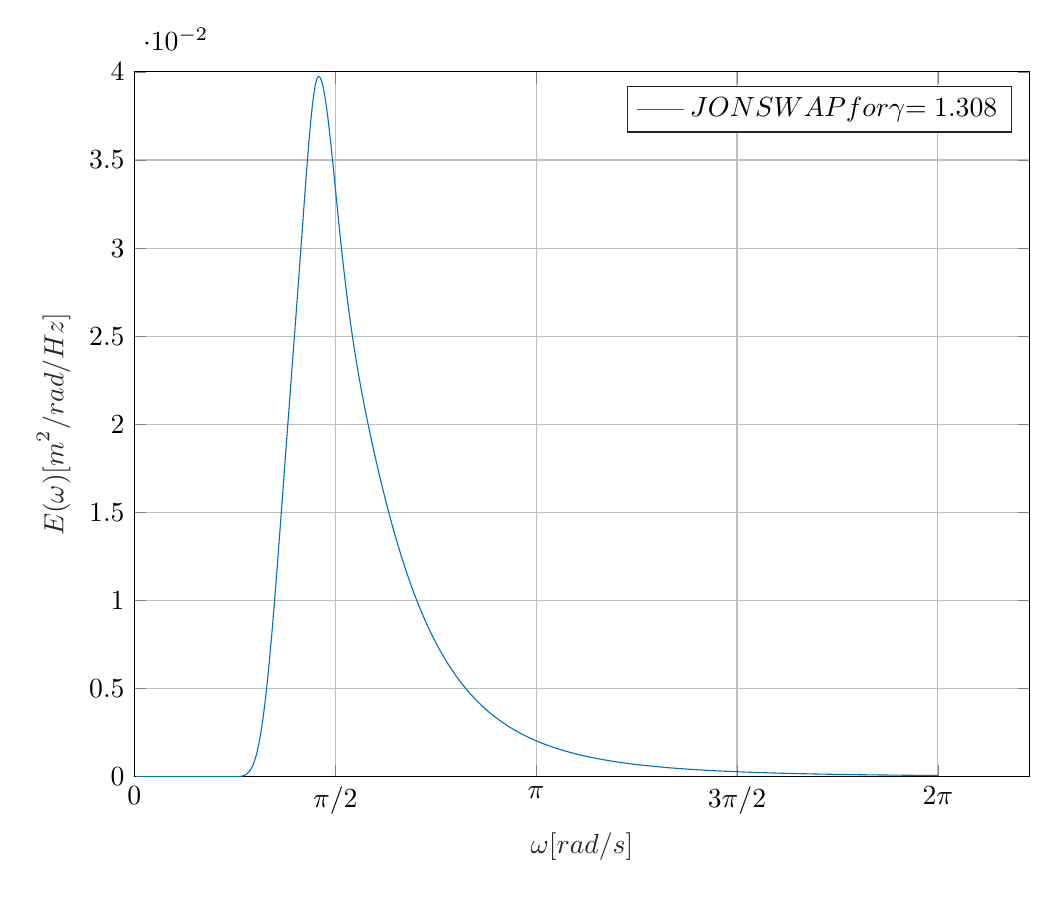
\begin{tikzpicture}

\begin{axis}[%
width=4.476in,
height=3.524in,
at={(0.803in,0.523in)},
scale only axis,
unbounded coords=jump,
xmin=0,
xmax=7,
xtick={0,1.5707963267949,3.14159265358979,4.71238898038469,6.28318530717959},
xticklabels={{0},{$\pi\text{/2}$},{$\pi$},{$\text{3}\pi\text{/2}$},{$\text{2}\pi$}},
xlabel style={font=\color{white!15!black}},
xlabel={$\omega\text{ [rad/s]}$},
ymin=0,
ymax=0.04,
ylabel style={font=\color{white!15!black}},
ylabel={$\text{E(}\omega\text{) [m}^\text{2}\text{/rad/Hz]}$},
axis background/.style={fill=white},
title style={font=\bfseries},
%title={$\text{One-dimensional wave spectrum, E(}\omega\text{) at -34S, 17.25E}$},
xmajorgrids,
ymajorgrids,
legend style={legend cell align=left, align=left, draw=white!15!black}
]
\addplot [color=mycolor1]
  table[row sep=crcr]{%
0	nan\\
0.0122958616578857	0\\
0.0245917233157714	0\\
0.0368875849736571	0\\
0.0491834466315427	0\\
0.0614793082894284	0\\
0.0737751699473141	0\\
0.0860710316051998	0\\
0.0983668932630855	0\\
0.110662754920971	0\\
0.122958616578857	0\\
0.135254478236743	0\\
0.147550339894628	0\\
0.159846201552514	0\\
0.1721420632104	0\\
0.184437924868285	0\\
0.196733786526171	0\\
0.209029648184057	0\\
0.221325509841942	0\\
0.233621371499828	0\\
0.245917233157714	0\\
0.258213094815599	0\\
0.270508956473485	0\\
0.282804818131371	0\\
0.295100679789256	5.41302879763333e-307\\
0.307396541447142	1.4351658983951e-260\\
0.319692403105028	1.39801651640755e-222\\
0.331988264762914	2.95955173493782e-191\\
0.344284126420799	3.06617261869068e-165\\
0.356579988078685	1.71585454184354e-143\\
0.368875849736571	3.36115162791715e-125\\
0.381171711394456	9.99471845091621e-110\\
0.393467573052342	1.44074967318733e-96\\
0.405763434710228	2.54134308132756e-85\\
0.418059296368113	1.15384979645612e-75\\
0.430355158025999	2.46010694641464e-67\\
0.442651019683885	4.01707121559874e-60\\
0.45494688134177	7.49671131280128e-54\\
0.467242742999656	2.22288404307939e-48\\
0.479538604657542	1.3753760835859e-43\\
0.491834466315427	2.22745866619101e-39\\
0.504130327973313	1.14105811314078e-35\\
0.516426189631199	2.16730148431401e-32\\
0.528722051289085	1.74501685936915e-29\\
0.54101791294697	6.67054290550385e-27\\
0.553313774604856	1.33294088654399e-24\\
0.565609636262742	1.51145852287043e-22\\
0.577905497920627	1.0433270916913e-20\\
0.590201359578513	4.65664898554377e-19\\
0.602497221236399	1.41551545559892e-17\\
0.614793082894284	3.06504085545376e-16\\
0.62708894455217	4.91508596715723e-15\\
0.639384806210056	6.03782647089776e-14\\
0.651680667867941	5.85166582657271e-13\\
0.663976529525827	4.59100381164424e-12\\
0.676272391183713	2.98235025750544e-11\\
0.688568252841599	1.63618607596188e-10\\
0.700864114499484	7.71435740175365e-10\\
0.71315997615737	3.17422780050511e-09\\
0.725455837815256	1.15545266932238e-08\\
0.737751699473141	3.76593918002615e-08\\
0.750047561131027	1.11082567474578e-07\\
0.762343422788913	2.99365257438456e-07\\
0.774639284446798	7.43398794457705e-07\\
0.786935146104684	1.71393732492197e-06\\
0.79923100776257	3.6936978163335e-06\\
0.811526869420455	7.48610717182671e-06\\
0.823822731078341	1.43464290828625e-05\\
0.836118592736227	2.61246562604755e-05\\
0.848414454394112	4.54036148623333e-05\\
0.860710316051998	7.56117606150625e-05\\
0.873006177709884	0.000121089372916668\\
0.88530203936777	0.000187089786772187\\
0.897597901025655	0.000279703606526386\\
0.909893762683541	0.000405702450085907\\
0.922189624341426	0.000572308176547121\\
0.934485485999312	0.000786902195884214\\
0.946781347657198	0.00105669606424971\\
0.959077209315084	0.00138838834019309\\
0.971373070972969	0.00178783338397504\\
0.983668932630855	0.00225974569705202\\
0.995964794288741	0.00280745915996462\\
1.00826065594663	0.00343275496464683\\
1.02055651760451	0.00413576600873186\\
1.0328523792624	0.00491495977802167\\
1.04514824092028	0.00576719685342651\\
1.05744410257817	0.00668785847600663\\
1.06973996423605	0.00767103419145496\\
1.08203582589394	0.00870975936699404\\
1.09433168755183	0.0097962920536587\\
1.10662754920971	0.0109224188636112\\
1.1189234108676	0.0120797798007726\\
1.13121927252548	0.0132602018978306\\
1.14351513418337	0.0144560307440969\\
1.15581099584125	0.0156604473784329\\
1.16810685749914	0.0168677556407375\\
1.18040271915703	0.0180736222488931\\
1.19269858081491	0.0192752491472963\\
1.2049944424728	0.0204714557558278\\
1.21729030413068	0.0216626483564445\\
1.22958616578857	0.0228506556097147\\
1.24188202744645	0.0240384135360737\\
1.25417788910434	0.0252294904939306\\
1.26647375076223	0.0264274529344006\\
1.27876961242011	0.0276350862726403\\
1.291065474078	0.0288535024756524\\
1.30336133573588	0.0300811872588852\\
1.31565719739377	0.0313130648442189\\
1.32795305905165	0.0325396852882558\\
1.34024892070954	0.0337466641153829\\
1.35254478236743	0.0349145188355605\\
1.36484064402531	0.0360190415875961\\
1.3771365056832	0.0370323108877261\\
1.38943236734108	0.0379243714742074\\
1.40172822899897	0.0386655021114703\\
1.41402409065685	0.0392288631897149\\
1.42631995231474	0.0395931988386078\\
1.43861581397263	0.0397451987880671\\
1.45091167563051	0.0397009837064543\\
1.4632075372884	0.0395060933162202\\
1.47550339894628	0.0391703952648501\\
1.48779926060417	0.0387059506556059\\
1.50009512226205	0.0381276193041899\\
1.51239098391994	0.0374522472133023\\
1.52468684557783	0.0366977905296433\\
1.53698270723571	0.0358824534634019\\
1.5492785688936	0.0350239067515314\\
1.56157443055148	0.0341386357865274\\
1.57387029220937	0.033241447182027\\
1.58616615386725	0.0323451427488864\\
1.59846201552514	0.0314603532066003\\
1.61075787718303	0.0305955119179262\\
1.62305373884091	0.0297569418708591\\
1.6353496004988	0.0289490265523619\\
1.64764546215668	0.0281744362672717\\
1.65994132381457	0.0274343846835443\\
1.67223718547245	0.0267288948374096\\
1.68453304713034	0.0260570586376697\\
1.69682890878822	0.0254172784703886\\
1.70912477044611	0.0248074834845985\\
1.721420632104	0.024225316400738\\
1.73371649376188	0.023668289227364\\
1.74601235541977	0.0231339081746281\\
1.75830821707765	0.0226197694201764\\
1.77060407873554	0.0221236283185714\\
1.78289994039342	0.0216434452374737\\
1.79519580205131	0.0211774115218765\\
1.8074916637092	0.0207239591846428\\
1.81978752536708	0.0202817578397189\\
1.83208338702497	0.0198497021705522\\
1.84437924868285	0.0194268928954684\\
1.85667511034074	0.0190126137886203\\
1.86897097199862	0.0186063068732881\\
1.88126683365651	0.0182075474549375\\
1.8935626953144	0.0178160202313337\\
1.90585855697228	0.0174314973270267\\
1.91815441863017	0.0170538187637728\\
1.93045028028805	0.0166828756042898\\
1.94274614194594	0.0163185957954444\\
1.95504200360382	0.0159609325850235\\
1.96733786526171	0.0156098552867384\\
1.9796337269196	0.015265342112225\\
1.99192958857748	0.0149273747670556\\
2.00422545023537	0.0145959345109985\\
2.01652131189325	0.0142709994027779\\
2.02881717355114	0.0139525424796016\\
2.04111303520902	0.0136405306563983\\
2.05340889686691	0.0133349241651845\\
2.0657047585248	0.0130356763886258\\
2.07800062018268	0.0127427339721329\\
2.09029648184057	0.0124560371249502\\
2.10259234349845	0.0121755200424896\\
2.11488820515634	0.0119011113998192\\
2.12718406681422	0.0116327348801607\\
2.13947992847211	0.011370309712995\\
2.15177579012999	0.0111137512044894\\
2.16407165178788	0.0108629712489418\\
2.17636751344577	0.0106178788142673\\
2.18866337510365	0.0103783803976124\\
2.20095923676154	0.0101443804493013\\
2.21325509841942	0.00991578176473845\\
2.22555096007731	0.00969248584482827\\
2.2378468217352	0.00947439322604724\\
2.25014268339308	0.00926140378164897\\
2.26243854505097	0.0090534169956585\\
2.27473440670885	0.00885033221138453\\
2.28703026836674	0.00865204885617913\\
2.29932613002462	0.00845846664413426\\
2.31162199168251	0.00826948575833719\\
2.3239178533404	0.00808500701422663\\
2.33621371499828	0.00790493200550391\\
2.34850957665617	0.00772916323396475\\
2.36080543831405	0.00755760422452847\\
2.37310129997194	0.00739015962665654\\
2.38539716162982	0.00722673530327022\\
2.39769302328771	0.00706723840819925\\
2.40998888494559	0.00691157745312068\\
2.42228474660348	0.0067596623648772\\
2.43458060826137	0.00661140453400037\\
2.44687646991925	0.00646671685520286\\
2.45917233157714	0.00632551376054758\\
2.47146819323502	0.00618771124594853\\
2.48376405489291	0.00605322689160874\\
2.49605991655079	0.00592197987695489\\
2.50835577820868	0.00579389099058502\\
2.52065163986657	0.00566888263570622\\
2.53294750152445	0.00554687883150177\\
2.54524336318234	0.00542780521083287\\
2.55753922484022	0.00531158901464808\\
2.56983508649811	0.00519815908344373\\
2.58213094815599	0.00508744584609102\\
2.59442680981388	0.00497938130631981\\
2.60672267147177	0.00487389902712567\\
2.61901853312965	0.00477093411334424\\
2.63131439478754	0.00467042319261705\\
2.64361025644542	0.00457230439495386\\
2.65590611810331	0.00447651733107909\\
2.66820197976119	0.00438300306973388\\
2.68049784141908	0.00429170411409041\\
2.69279370307697	0.00420256437742111\\
2.70508956473485	0.00411552915815301\\
2.71738542639274	0.00403054511442532\\
2.72968128805062	0.00394756023825787\\
2.74197714970851	0.00386652382942774\\
2.75427301136639	0.00378738646914243\\
2.76656887302428	0.00371009999358922\\
2.77886473468217	0.00363461746743274\\
2.79116059634005	0.00356089315732546\\
2.80345645799794	0.00348888250548924\\
2.81575231965582	0.00341854210342006\\
2.82804818131371	0.00334982966576232\\
2.84034404297159	0.00328270400439414\\
2.85263990462948	0.00321712500276036\\
2.86493576628737	0.00315305359048552\\
2.87723162794525	0.00309045171829528\\
2.88952748960314	0.00302928233327117\\
2.90182335126102	0.0029695093544601\\
2.91411921291891	0.00291109764885714\\
2.92641507457679	0.00285401300777748\\
2.93871093623468	0.00279822212363068\\
2.95100679789256	0.00274369256710825\\
2.96330265955045	0.00269039276479353\\
2.97559852120834	0.00263829197720089\\
2.98789438286622	0.00258736027724954\\
3.00019024452411	0.00253756852917576\\
3.01248610618199	0.00248888836788607\\
3.02478196783988	0.00244129217875227\\
3.03707782949776	0.00239475307784859\\
3.04937369115565	0.00234924489262979\\
3.06166955281354	0.0023047421430484\\
3.07396541447142	0.0022612200231083\\
3.08626127612931	0.00221865438285134\\
3.09855713778719	0.00217702171077273\\
3.11085299944508	0.00213629911666074\\
3.12314886110296	0.00209646431485547\\
3.13544472276085	0.00205749560792113\\
3.14774058441874	0.00201937187072593\\
3.16003644607662	0.00198207253492326\\
3.17233230773451	0.00194557757382764\\
3.18462816939239	0.00190986748767868\\
3.19692403105028	0.00187492328928602\\
3.20921989270816	0.00184072649004824\\
3.22151575436605	0.00180725908633834\\
3.23381161602394	0.00177450354624858\\
3.24610747768182	0.00174244279668723\\
3.25840333933971	0.00171106021081969\\
3.27069920099759	0.0016803395958467\\
3.28299506265548	0.00165026518111192\\
3.29529092431336	0.00162082160653164\\
3.30758678597125	0.00159199391133908\\
3.31988264762914	0.00156376752313587\\
3.33217850928702	0.00153612824724346\\
3.34447437094491	0.00150906225634721\\
3.35677023260279	0.00148255608042589\\
3.36906609426068	0.00145659659695957\\
3.38136195591856	0.00143117102140895\\
3.39365781757645	0.00140626689795909\\
3.40595367923434	0.00138187209052092\\
3.41824954089222	0.00135797477398379\\
3.43054540255011	0.00133456342571239\\
3.44284126420799	0.00131162681728186\\
3.45513712586588	0.00128915400644448\\
3.46743298752376	0.00126713432932197\\
3.47972884918165	0.00124555739281723\\
3.49202471083954	0.00122441306723957\\
3.50432057249742	0.00120369147913769\\
3.51661643415531	0.00118338300433464\\
3.52891229581319	0.00116347826115928\\
3.54120815747108	0.00114396810386871\\
3.55350401912896	0.00112484361625655\\
3.56579988078685	0.0011060961054416\\
3.57809574244473	0.00108771709583218\\
3.59039160410262	0.00106969832326091\\
3.60268746576051	0.00105203172928534\\
3.61498332741839	0.00103470945564963\\
3.62727918907628	0.0010177238389028\\
3.63957505073416	0.00100106740516895\\
3.65187091239205	0.000984732865065375\\
3.66416677404994	0.000968713108764074\\
3.67646263570782	0.00095300120119279\\
3.68875849736571	0.00093759037737141\\
3.70105435902359	0.000922474037879949\\
3.71335022068148	0.000907645744454282\\
3.72564608233936	0.000893099215705966\\
3.73794194399725	0.000878828322962575\\
3.75023780565513	0.000864827086225059\\
3.76253366731302	0.000851089670238769\\
3.77482952897091	0.000837610380674829\\
3.78712539062879	0.000824383660418703\\
3.79942125228668	0.000811404085962812\\
3.81171711394456	0.00079866636390022\\
3.82401297560245	0.000786165327516438\\
3.83630883726033	0.000773895933476511\\
3.84860469891822	0.000761853258604621\\
3.86090056057611	0.000750032496753526\\
3.87319642223399	0.000738428955761214\\
3.88549228389188	0.000727038054492271\\
3.89778814554976	0.000715855319961465\\
3.91008400720765	0.000704876384537197\\
3.92237986886553	0.000694096983222478\\
3.93467573052342	0.000683512951011199\\
3.94697159218131	0.000673120220317491\\
3.95926745383919	0.000662914818476088\\
3.97156331549708	0.000652892865311599\\
3.98385917715496	0.000643050570774724\\
3.99615503881285	0.000633384232643455\\
4.00845090047073	0.000623890234287399\\
4.02074676212862	0.000614565042493382\\
4.03304262378651	0.000605405205350579\\
4.04533848544439	0.000596407350193436\\
4.05763434710228	0.000587568181600735\\
4.06993020876016	0.000578884479449159\\
4.08222607041805	0.00057035309701982\\
4.09452193207593	0.000561970959156189\\
4.10681779373382	0.000553735060471986\\
4.1191136553917	0.000545642463607562\\
4.13140951704959	0.000537690297533413\\
4.14370537870748	0.00052987575589945\\
4.15600124036536	0.000522196095428724\\
4.16829710202325	0.000514648634354346\\
4.18059296368113	0.00050723075089834\\
4.19288882533902	0.00049993988179127\\
4.2051846869969	0.000492773520831441\\
4.21748054865479	0.00048572921748257\\
4.22977641031268	0.000478804575508837\\
4.24207227197056	0.000471997251646233\\
4.25436813362845	0.000465304954309197\\
4.26666399528633	0.000458725442331523\\
4.27895985694422	0.000452256523740597\\
4.29125571860211	0.000445896054563984\\
4.30355158025999	0.000439641937667487\\
4.31584744191788	0.000433492121623766\\
4.32814330357576	0.000427444599610678\\
4.34043916523365	0.000421497408338488\\
4.35273502689153	0.000415648627005148\\
4.36503088854942	0.000409896376278856\\
4.37732675020731	0.000404238817307136\\
4.38962261186519	0.000398674150751693\\
4.40191847352308	0.000393200615848326\\
4.41421433518096	0.000387816489491206\\
4.42651019683885	0.000382520085340833\\
4.43880605849673	0.000377309752955029\\
4.45110192015462	0.000372183876942308\\
4.46339778181251	0.000367140876137024\\
4.47569364347039	0.000362179202795692\\
4.48798950512828	0.000357297341813879\\
4.50028536678616	0.000352493809963128\\
4.51258122844405	0.000347767155147345\\
4.52487709010193	0.000343115955678117\\
4.53717295175982	0.000338538819568452\\
4.5494688134177	0.000334034383844427\\
4.56176467507559	0.000329601313874257\\
4.57406053673348	0.000325238302714321\\
4.58635639839136	0.000320944070471665\\
4.59865226004925	0.000316717363682552\\
4.61094812170713	0.000312556954706612\\
4.62324398336502	0.00030846164113618\\
4.6355398450229	0.000304430245220401\\
4.64783570668079	0.000300461613303707\\
4.66013156833868	0.000296554615278295\\
4.67242742999656	0.000292708144050196\\
4.68472329165445	0.000288921115018604\\
4.69701915331233	0.000285192465568094\\
4.70931501497022	0.000281521154573383\\
4.7216108766281	0.000277906161916305\\
4.73390673828599	0.000274346488014674\\
4.74620259994388	0.000270841153362717\\
4.75849846160176	0.000267389198082769\\
4.77079432325965	0.000263989681487935\\
4.78309018491753	0.000260641681655428\\
4.79538604657542	0.000257344295010299\\
4.8076819082333	0.000254096635919287\\
4.81997776989119	0.000250897836294526\\
4.83227363154908	0.000247747045206839\\
4.84456949320696	0.000244643428508389\\
4.85686535486485	0.000241586168464416\\
4.86916121652273	0.000238574463393844\\
4.88145707818062	0.000235607527318515\\
4.8937529398385	0.000232684589620834\\
4.90604880149639	0.000229804894709597\\
4.91834466315427	0.000226967701693801\\
4.93064052481216	0.000224172284064218\\
4.94293638647005	0.000221417929382543\\
4.95523224812793	0.000218703938977918\\
4.96752810978582	0.000216029627650631\\
4.9798239714437	0.000213394323382829\\
4.99211983310159	0.000210797367056043\\
5.00441569475948	0.000208238112175362\\
5.01671155641736	0.000205715924600084\\
5.02900741807525	0.000203230182280682\\
5.04130327973313	0.000200780275001916\\
5.05359914139102	0.000198365604131947\\
5.0658950030489	0.000195985582377289\\
5.07819086470679	0.00019363963354346\\
5.09048672636467	0.000191327192301187\\
5.10278258802256	0.000189047703958018\\
5.11507844968045	0.000186800624235214\\
5.12737431133833	0.00018458541904979\\
5.13967017299622	0.000182401564301559\\
5.1519660346541	0.000180248545665076\\
5.16426189631199	0.000178125858386348\\
5.17655775796987	0.000176033007084189\\
5.18885361962776	0.000173969505556115\\
5.20114948128565	0.000171934876588657\\
5.21344534294353	0.000169928651771981\\
5.22574120460142	0.000167950371318724\\
5.2380370662593	0.000165999583886923\\
5.25033292791719	0.000164075846406948\\
5.26262878957507	0.000162178723912337\\
5.27492465123296	0.000160307789374435\\
5.28722051289085	0.000158462623540752\\
5.29951637454873	0.000156642814776941\\
5.31181223620662	0.000154847958912307\\
5.3241080978645	0.000153077659088771\\
5.33640395952239	0.000151331525613192\\
5.34869982118027	0.000149609175812981\\
5.36099568283816	0.000147910233894908\\
5.37329154449605	0.000146234330807043\\
5.38558740615393	0.000144581104103749\\
5.39788326781182	0.000142950197813643\\
5.4101791294697	0.000141341262310475\\
5.42247499112759	0.000139753954186838\\
5.43477085278547	0.000138187936130644\\
5.44706671444336	0.000136642876804307\\
5.45936257610125	0.000135118450726565\\
5.47165843775913	0.000133614338156872\\
5.48395429941702	0.00013213022498231\\
5.4962501610749	0.00013066580260695\\
5.50854602273279	0.000129220767843618\\
5.52084188439067	0.000127794822807993\\
5.53313774604856	0.000126387674814993\\
5.54543360770645	0.000124999036277395\\
5.55772946936433	0.000123628624606628\\
5.57002533102222	0.000122276162115703\\
5.5823211926801	0.00012094137592421\\
5.59461705433799	0.000119623997865353\\
5.60691291599587	0.000118323764394966\\
5.61920877765376	0.00011704041650246\\
5.63150463931164	0.000115773699623671\\
5.64380050096953	0.000114523363555545\\
5.65609636262742	0.000113289162372638\\
5.6683922242853	0.00011207085434537\\
5.68068808594319	0.000110868201860007\\
5.69298394760107	0.000109680971340328\\
5.70527980925896	0.00010850893317093\\
5.71757567091684	0.000107351861622146\\
5.72987153257473	0.000106209534776526\\
5.74216739423262	0.000105081734456864\\
5.7544632558905	0.000103968246155711\\
5.76675911754839	0.000102868858966361\\
5.77905497920627	0.000101783365515268\\
5.79135084086416	0.000100711561895862\\
5.80364670252204	9.96532476037344e-05\\
5.81594256417993	9.86082254731543e-05\\
5.82823842583782	9.75763016149018e-05\\
5.8405342874957	9.65572853553714e-05\\
5.85283014915359	9.55509891769276e-05\\
5.86512601081147	9.455722865948e-05\\
5.87742187246936	9.35758224232536e-05\\
5.88971773412724	9.26065920727251e-05\\
5.90201359578513	9.16493621417014e-05\\
5.91430945744302	9.07039600395125e-05\\
5.9266053191009	8.97702159982964e-05\\
5.93890118075879	8.88479630213512e-05\\
5.95119704241667	8.79370368325295e-05\\
5.96349290407456	8.70372758266536e-05\\
5.97578876573244	8.61485210209284e-05\\
5.98808462739033	8.5270616007331e-05\\
6.00038048904822	8.4403406905953e-05\\
6.0126763507061	8.35467423192785e-05\\
6.02497221236399	8.27004732873734e-05\\
6.03726807402187	8.18644532439695e-05\\
6.04956393567976	8.10385379734214e-05\\
6.06185979733764	8.02225855685183e-05\\
6.07415565899553	7.94164563891332e-05\\
6.08645152065342	7.86200130216882e-05\\
6.0987473823113	7.78331202394225e-05\\
6.11104324396919	7.70556449634419e-05\\
6.12333910562707	7.62874562245356e-05\\
6.13563496728496	7.55284251257423e-05\\
6.14793082894284	7.4778424805651e-05\\
6.16022669060073	7.40373304024179e-05\\
6.17252255225862	7.33050190184887e-05\\
6.1848184139165	7.25813696860062e-05\\
6.19711427557439	7.18662633328921e-05\\
6.20941013723227	7.11595827495877e-05\\
6.22170599889016	7.04612125564384e-05\\
6.23400186054804	6.97710391717103e-05\\
6.24629772220593	6.90889507802242e-05\\
6.25859358386381	6.84148373025936e-05\\
6.2708894455217	6.77485903650559e-05\\
6.28318530717959	6.70901032698821e-05\\
};
\addlegendentry{$\text{JONSWAP for }\gamma\text{ = 1.308}$}

\end{axis}
\end{tikzpicture}%}
%     \caption{\acs{jonswap} spectrum at -34S, 17.25E}
%     \label{fig:systemDesign.1DSampleWaveSpectrumSingle}   
% \end{subfigure}
% \begin{subfigure}{0.48\linewidth} % Use \begin{subfigure} instead of \begin{subfigure}
%     \resizebox{\linewidth}{!}{% This file was created by matlab2tikz.
%
%The latest updates can be retrieved from
%  http://www.mathworks.com/matlabcentral/fileexchange/22022-matlab2tikz-matlab2tikz
%where you can also make suggestions and rate matlab2tikz.
%
\definecolor{mycolor1}{rgb}{0.00000,0.44700,0.74100}%
\definecolor{mycolor2}{rgb}{0.85000,0.32500,0.09800}%
\definecolor{mycolor3}{rgb}{0.92900,0.69400,0.12500}%
%
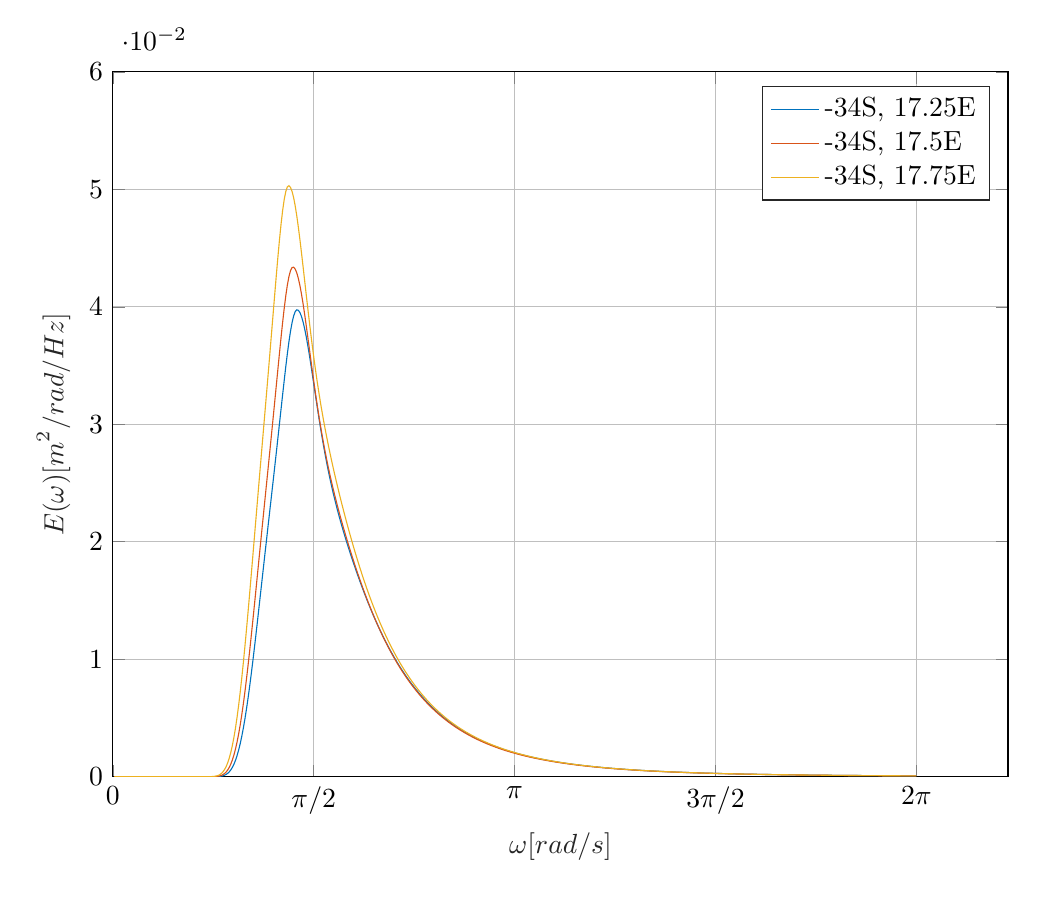
\begin{tikzpicture}

\begin{axis}[%
width=4.476in,
height=3.524in,
at={(0.803in,0.523in)},
scale only axis,
unbounded coords=jump,
xmin=0,
xmax=7,
xtick={0,1.5707963267949,3.14159265358979,4.71238898038469,6.28318530717959},
xticklabels={{0},{$\pi\text{/2}$},{$\pi$},{$\text{3}\pi\text{/2}$},{$\text{2}\pi$}},
xlabel style={font=\color{white!15!black}},
xlabel={$\omega\text{ [rad/s]}$},
ymin=0,
ymax=0.06,
ylabel style={font=\color{white!15!black}},
ylabel={$\text{E(}\omega\text{) [m}^\text{2}\text{/rad/Hz]}$},
axis background/.style={fill=white},
title style={font=\bfseries},
xmajorgrids,
ymajorgrids,
legend style={legend cell align=left, align=left, draw=white!15!black}
]
\addplot [color=mycolor1]
  table[row sep=crcr]{%
0	nan\\
0.0122958616578857	0\\
0.0245917233157714	0\\
0.0368875849736571	0\\
0.0491834466315427	0\\
0.0614793082894284	0\\
0.0737751699473141	0\\
0.0860710316051998	0\\
0.0983668932630855	0\\
0.110662754920971	0\\
0.122958616578857	0\\
0.135254478236743	0\\
0.147550339894628	0\\
0.159846201552514	0\\
0.1721420632104	0\\
0.184437924868285	0\\
0.196733786526171	0\\
0.209029648184057	0\\
0.221325509841942	0\\
0.233621371499828	0\\
0.245917233157714	0\\
0.258213094815599	0\\
0.270508956473485	0\\
0.282804818131371	0\\
0.295100679789256	5.41302879763333e-307\\
0.307396541447142	1.4351658983951e-260\\
0.319692403105028	1.39801651640755e-222\\
0.331988264762914	2.95955173493782e-191\\
0.344284126420799	3.06617261869068e-165\\
0.356579988078685	1.71585454184354e-143\\
0.368875849736571	3.36115162791715e-125\\
0.381171711394456	9.99471845091621e-110\\
0.393467573052342	1.44074967318733e-96\\
0.405763434710228	2.54134308132756e-85\\
0.418059296368113	1.15384979645612e-75\\
0.430355158025999	2.46010694641464e-67\\
0.442651019683885	4.01707121559874e-60\\
0.45494688134177	7.49671131280128e-54\\
0.467242742999656	2.22288404307939e-48\\
0.479538604657542	1.3753760835859e-43\\
0.491834466315427	2.22745866619101e-39\\
0.504130327973313	1.14105811314078e-35\\
0.516426189631199	2.16730148431401e-32\\
0.528722051289085	1.74501685936915e-29\\
0.54101791294697	6.67054290550385e-27\\
0.553313774604856	1.33294088654399e-24\\
0.565609636262742	1.51145852287043e-22\\
0.577905497920627	1.0433270916913e-20\\
0.590201359578513	4.65664898554377e-19\\
0.602497221236399	1.41551545559892e-17\\
0.614793082894284	3.06504085545376e-16\\
0.62708894455217	4.91508596715723e-15\\
0.639384806210056	6.03782647089776e-14\\
0.651680667867941	5.85166582657271e-13\\
0.663976529525827	4.59100381164424e-12\\
0.676272391183713	2.98235025750544e-11\\
0.688568252841599	1.63618607596188e-10\\
0.700864114499484	7.71435740175365e-10\\
0.71315997615737	3.17422780050511e-09\\
0.725455837815256	1.15545266932238e-08\\
0.737751699473141	3.76593918002615e-08\\
0.750047561131027	1.11082567474578e-07\\
0.762343422788913	2.99365257438456e-07\\
0.774639284446798	7.43398794457705e-07\\
0.786935146104684	1.71393732492197e-06\\
0.79923100776257	3.6936978163335e-06\\
0.811526869420455	7.48610717182671e-06\\
0.823822731078341	1.43464290828625e-05\\
0.836118592736227	2.61246562604755e-05\\
0.848414454394112	4.54036148623333e-05\\
0.860710316051998	7.56117606150625e-05\\
0.873006177709884	0.000121089372916668\\
0.88530203936777	0.000187089786772187\\
0.897597901025655	0.000279703606526386\\
0.909893762683541	0.000405702450085907\\
0.922189624341426	0.000572308176547121\\
0.934485485999312	0.000786902195884214\\
0.946781347657198	0.00105669606424971\\
0.959077209315084	0.00138838834019309\\
0.971373070972969	0.00178783338397504\\
0.983668932630855	0.00225974569705202\\
0.995964794288741	0.00280745915996462\\
1.00826065594663	0.00343275496464683\\
1.02055651760451	0.00413576600873186\\
1.0328523792624	0.00491495977802167\\
1.04514824092028	0.00576719685342651\\
1.05744410257817	0.00668785847600663\\
1.06973996423605	0.00767103419145496\\
1.08203582589394	0.00870975936699404\\
1.09433168755183	0.0097962920536587\\
1.10662754920971	0.0109224188636112\\
1.1189234108676	0.0120797798007726\\
1.13121927252548	0.0132602018978306\\
1.14351513418337	0.0144560307440969\\
1.15581099584125	0.0156604473784329\\
1.16810685749914	0.0168677556407375\\
1.18040271915703	0.0180736222488931\\
1.19269858081491	0.0192752491472963\\
1.2049944424728	0.0204714557558278\\
1.21729030413068	0.0216626483564445\\
1.22958616578857	0.0228506556097147\\
1.24188202744645	0.0240384135360737\\
1.25417788910434	0.0252294904939306\\
1.26647375076223	0.0264274529344006\\
1.27876961242011	0.0276350862726403\\
1.291065474078	0.0288535024756524\\
1.30336133573588	0.0300811872588852\\
1.31565719739377	0.0313130648442189\\
1.32795305905165	0.0325396852882558\\
1.34024892070954	0.0337466641153829\\
1.35254478236743	0.0349145188355605\\
1.36484064402531	0.0360190415875961\\
1.3771365056832	0.0370323108877261\\
1.38943236734108	0.0379243714742074\\
1.40172822899897	0.0386655021114703\\
1.41402409065685	0.0392288631897149\\
1.42631995231474	0.0395931988386078\\
1.43861581397263	0.0397451987880671\\
1.45091167563051	0.0397009837064543\\
1.4632075372884	0.0395060933162202\\
1.47550339894628	0.0391703952648501\\
1.48779926060417	0.0387059506556059\\
1.50009512226205	0.0381276193041899\\
1.51239098391994	0.0374522472133023\\
1.52468684557783	0.0366977905296433\\
1.53698270723571	0.0358824534634019\\
1.5492785688936	0.0350239067515314\\
1.56157443055148	0.0341386357865274\\
1.57387029220937	0.033241447182027\\
1.58616615386725	0.0323451427488864\\
1.59846201552514	0.0314603532066003\\
1.61075787718303	0.0305955119179262\\
1.62305373884091	0.0297569418708591\\
1.6353496004988	0.0289490265523619\\
1.64764546215668	0.0281744362672717\\
1.65994132381457	0.0274343846835443\\
1.67223718547245	0.0267288948374096\\
1.68453304713034	0.0260570586376697\\
1.69682890878822	0.0254172784703886\\
1.70912477044611	0.0248074834845985\\
1.721420632104	0.024225316400738\\
1.73371649376188	0.023668289227364\\
1.74601235541977	0.0231339081746281\\
1.75830821707765	0.0226197694201764\\
1.77060407873554	0.0221236283185714\\
1.78289994039342	0.0216434452374737\\
1.79519580205131	0.0211774115218765\\
1.8074916637092	0.0207239591846428\\
1.81978752536708	0.0202817578397189\\
1.83208338702497	0.0198497021705522\\
1.84437924868285	0.0194268928954684\\
1.85667511034074	0.0190126137886203\\
1.86897097199862	0.0186063068732881\\
1.88126683365651	0.0182075474549375\\
1.8935626953144	0.0178160202313337\\
1.90585855697228	0.0174314973270267\\
1.91815441863017	0.0170538187637728\\
1.93045028028805	0.0166828756042898\\
1.94274614194594	0.0163185957954444\\
1.95504200360382	0.0159609325850235\\
1.96733786526171	0.0156098552867384\\
1.9796337269196	0.015265342112225\\
1.99192958857748	0.0149273747670556\\
2.00422545023537	0.0145959345109985\\
2.01652131189325	0.0142709994027779\\
2.02881717355114	0.0139525424796016\\
2.04111303520902	0.0136405306563983\\
2.05340889686691	0.0133349241651845\\
2.0657047585248	0.0130356763886258\\
2.07800062018268	0.0127427339721329\\
2.09029648184057	0.0124560371249502\\
2.10259234349845	0.0121755200424896\\
2.11488820515634	0.0119011113998192\\
2.12718406681422	0.0116327348801607\\
2.13947992847211	0.011370309712995\\
2.15177579012999	0.0111137512044894\\
2.16407165178788	0.0108629712489418\\
2.17636751344577	0.0106178788142673\\
2.18866337510365	0.0103783803976124\\
2.20095923676154	0.0101443804493013\\
2.21325509841942	0.00991578176473845\\
2.22555096007731	0.00969248584482827\\
2.2378468217352	0.00947439322604724\\
2.25014268339308	0.00926140378164897\\
2.26243854505097	0.0090534169956585\\
2.27473440670885	0.00885033221138453\\
2.28703026836674	0.00865204885617913\\
2.29932613002462	0.00845846664413426\\
2.31162199168251	0.00826948575833719\\
2.3239178533404	0.00808500701422663\\
2.33621371499828	0.00790493200550391\\
2.34850957665617	0.00772916323396475\\
2.36080543831405	0.00755760422452847\\
2.37310129997194	0.00739015962665654\\
2.38539716162982	0.00722673530327022\\
2.39769302328771	0.00706723840819925\\
2.40998888494559	0.00691157745312068\\
2.42228474660348	0.0067596623648772\\
2.43458060826137	0.00661140453400037\\
2.44687646991925	0.00646671685520286\\
2.45917233157714	0.00632551376054758\\
2.47146819323502	0.00618771124594853\\
2.48376405489291	0.00605322689160874\\
2.49605991655079	0.00592197987695489\\
2.50835577820868	0.00579389099058502\\
2.52065163986657	0.00566888263570622\\
2.53294750152445	0.00554687883150177\\
2.54524336318234	0.00542780521083287\\
2.55753922484022	0.00531158901464808\\
2.56983508649811	0.00519815908344373\\
2.58213094815599	0.00508744584609102\\
2.59442680981388	0.00497938130631981\\
2.60672267147177	0.00487389902712567\\
2.61901853312965	0.00477093411334424\\
2.63131439478754	0.00467042319261705\\
2.64361025644542	0.00457230439495386\\
2.65590611810331	0.00447651733107909\\
2.66820197976119	0.00438300306973388\\
2.68049784141908	0.00429170411409041\\
2.69279370307697	0.00420256437742111\\
2.70508956473485	0.00411552915815301\\
2.71738542639274	0.00403054511442532\\
2.72968128805062	0.00394756023825787\\
2.74197714970851	0.00386652382942774\\
2.75427301136639	0.00378738646914243\\
2.76656887302428	0.00371009999358922\\
2.77886473468217	0.00363461746743274\\
2.79116059634005	0.00356089315732546\\
2.80345645799794	0.00348888250548924\\
2.81575231965582	0.00341854210342006\\
2.82804818131371	0.00334982966576232\\
2.84034404297159	0.00328270400439414\\
2.85263990462948	0.00321712500276036\\
2.86493576628737	0.00315305359048552\\
2.87723162794525	0.00309045171829528\\
2.88952748960314	0.00302928233327117\\
2.90182335126102	0.0029695093544601\\
2.91411921291891	0.00291109764885714\\
2.92641507457679	0.00285401300777748\\
2.93871093623468	0.00279822212363068\\
2.95100679789256	0.00274369256710825\\
2.96330265955045	0.00269039276479353\\
2.97559852120834	0.00263829197720089\\
2.98789438286622	0.00258736027724954\\
3.00019024452411	0.00253756852917576\\
3.01248610618199	0.00248888836788607\\
3.02478196783988	0.00244129217875227\\
3.03707782949776	0.00239475307784859\\
3.04937369115565	0.00234924489262979\\
3.06166955281354	0.0023047421430484\\
3.07396541447142	0.0022612200231083\\
3.08626127612931	0.00221865438285134\\
3.09855713778719	0.00217702171077273\\
3.11085299944508	0.00213629911666074\\
3.12314886110296	0.00209646431485547\\
3.13544472276085	0.00205749560792113\\
3.14774058441874	0.00201937187072593\\
3.16003644607662	0.00198207253492326\\
3.17233230773451	0.00194557757382764\\
3.18462816939239	0.00190986748767868\\
3.19692403105028	0.00187492328928602\\
3.20921989270816	0.00184072649004824\\
3.22151575436605	0.00180725908633834\\
3.23381161602394	0.00177450354624858\\
3.24610747768182	0.00174244279668723\\
3.25840333933971	0.00171106021081969\\
3.27069920099759	0.0016803395958467\\
3.28299506265548	0.00165026518111192\\
3.29529092431336	0.00162082160653164\\
3.30758678597125	0.00159199391133908\\
3.31988264762914	0.00156376752313587\\
3.33217850928702	0.00153612824724346\\
3.34447437094491	0.00150906225634721\\
3.35677023260279	0.00148255608042589\\
3.36906609426068	0.00145659659695957\\
3.38136195591856	0.00143117102140895\\
3.39365781757645	0.00140626689795909\\
3.40595367923434	0.00138187209052092\\
3.41824954089222	0.00135797477398379\\
3.43054540255011	0.00133456342571239\\
3.44284126420799	0.00131162681728186\\
3.45513712586588	0.00128915400644448\\
3.46743298752376	0.00126713432932197\\
3.47972884918165	0.00124555739281723\\
3.49202471083954	0.00122441306723957\\
3.50432057249742	0.00120369147913769\\
3.51661643415531	0.00118338300433464\\
3.52891229581319	0.00116347826115928\\
3.54120815747108	0.00114396810386871\\
3.55350401912896	0.00112484361625655\\
3.56579988078685	0.0011060961054416\\
3.57809574244473	0.00108771709583218\\
3.59039160410262	0.00106969832326091\\
3.60268746576051	0.00105203172928534\\
3.61498332741839	0.00103470945564963\\
3.62727918907628	0.0010177238389028\\
3.63957505073416	0.00100106740516895\\
3.65187091239205	0.000984732865065375\\
3.66416677404994	0.000968713108764074\\
3.67646263570782	0.00095300120119279\\
3.68875849736571	0.00093759037737141\\
3.70105435902359	0.000922474037879949\\
3.71335022068148	0.000907645744454282\\
3.72564608233936	0.000893099215705966\\
3.73794194399725	0.000878828322962575\\
3.75023780565513	0.000864827086225059\\
3.76253366731302	0.000851089670238769\\
3.77482952897091	0.000837610380674829\\
3.78712539062879	0.000824383660418703\\
3.79942125228668	0.000811404085962812\\
3.81171711394456	0.00079866636390022\\
3.82401297560245	0.000786165327516438\\
3.83630883726033	0.000773895933476511\\
3.84860469891822	0.000761853258604621\\
3.86090056057611	0.000750032496753526\\
3.87319642223399	0.000738428955761214\\
3.88549228389188	0.000727038054492271\\
3.89778814554976	0.000715855319961465\\
3.91008400720765	0.000704876384537197\\
3.92237986886553	0.000694096983222478\\
3.93467573052342	0.000683512951011199\\
3.94697159218131	0.000673120220317491\\
3.95926745383919	0.000662914818476088\\
3.97156331549708	0.000652892865311599\\
3.98385917715496	0.000643050570774724\\
3.99615503881285	0.000633384232643455\\
4.00845090047073	0.000623890234287399\\
4.02074676212862	0.000614565042493382\\
4.03304262378651	0.000605405205350579\\
4.04533848544439	0.000596407350193436\\
4.05763434710228	0.000587568181600735\\
4.06993020876016	0.000578884479449159\\
4.08222607041805	0.00057035309701982\\
4.09452193207593	0.000561970959156189\\
4.10681779373382	0.000553735060471986\\
4.1191136553917	0.000545642463607562\\
4.13140951704959	0.000537690297533413\\
4.14370537870748	0.00052987575589945\\
4.15600124036536	0.000522196095428724\\
4.16829710202325	0.000514648634354346\\
4.18059296368113	0.00050723075089834\\
4.19288882533902	0.00049993988179127\\
4.2051846869969	0.000492773520831441\\
4.21748054865479	0.00048572921748257\\
4.22977641031268	0.000478804575508837\\
4.24207227197056	0.000471997251646233\\
4.25436813362845	0.000465304954309197\\
4.26666399528633	0.000458725442331523\\
4.27895985694422	0.000452256523740597\\
4.29125571860211	0.000445896054563984\\
4.30355158025999	0.000439641937667487\\
4.31584744191788	0.000433492121623766\\
4.32814330357576	0.000427444599610678\\
4.34043916523365	0.000421497408338488\\
4.35273502689153	0.000415648627005148\\
4.36503088854942	0.000409896376278856\\
4.37732675020731	0.000404238817307136\\
4.38962261186519	0.000398674150751693\\
4.40191847352308	0.000393200615848326\\
4.41421433518096	0.000387816489491206\\
4.42651019683885	0.000382520085340833\\
4.43880605849673	0.000377309752955029\\
4.45110192015462	0.000372183876942308\\
4.46339778181251	0.000367140876137024\\
4.47569364347039	0.000362179202795692\\
4.48798950512828	0.000357297341813879\\
4.50028536678616	0.000352493809963128\\
4.51258122844405	0.000347767155147345\\
4.52487709010193	0.000343115955678117\\
4.53717295175982	0.000338538819568452\\
4.5494688134177	0.000334034383844427\\
4.56176467507559	0.000329601313874257\\
4.57406053673348	0.000325238302714321\\
4.58635639839136	0.000320944070471665\\
4.59865226004925	0.000316717363682552\\
4.61094812170713	0.000312556954706612\\
4.62324398336502	0.00030846164113618\\
4.6355398450229	0.000304430245220401\\
4.64783570668079	0.000300461613303707\\
4.66013156833868	0.000296554615278295\\
4.67242742999656	0.000292708144050196\\
4.68472329165445	0.000288921115018604\\
4.69701915331233	0.000285192465568094\\
4.70931501497022	0.000281521154573383\\
4.7216108766281	0.000277906161916305\\
4.73390673828599	0.000274346488014674\\
4.74620259994388	0.000270841153362717\\
4.75849846160176	0.000267389198082769\\
4.77079432325965	0.000263989681487935\\
4.78309018491753	0.000260641681655428\\
4.79538604657542	0.000257344295010299\\
4.8076819082333	0.000254096635919287\\
4.81997776989119	0.000250897836294526\\
4.83227363154908	0.000247747045206839\\
4.84456949320696	0.000244643428508389\\
4.85686535486485	0.000241586168464416\\
4.86916121652273	0.000238574463393844\\
4.88145707818062	0.000235607527318515\\
4.8937529398385	0.000232684589620834\\
4.90604880149639	0.000229804894709597\\
4.91834466315427	0.000226967701693801\\
4.93064052481216	0.000224172284064218\\
4.94293638647005	0.000221417929382543\\
4.95523224812793	0.000218703938977918\\
4.96752810978582	0.000216029627650631\\
4.9798239714437	0.000213394323382829\\
4.99211983310159	0.000210797367056043\\
5.00441569475948	0.000208238112175362\\
5.01671155641736	0.000205715924600084\\
5.02900741807525	0.000203230182280682\\
5.04130327973313	0.000200780275001916\\
5.05359914139102	0.000198365604131947\\
5.0658950030489	0.000195985582377289\\
5.07819086470679	0.00019363963354346\\
5.09048672636467	0.000191327192301187\\
5.10278258802256	0.000189047703958018\\
5.11507844968045	0.000186800624235214\\
5.12737431133833	0.00018458541904979\\
5.13967017299622	0.000182401564301559\\
5.1519660346541	0.000180248545665076\\
5.16426189631199	0.000178125858386348\\
5.17655775796987	0.000176033007084189\\
5.18885361962776	0.000173969505556115\\
5.20114948128565	0.000171934876588657\\
5.21344534294353	0.000169928651771981\\
5.22574120460142	0.000167950371318724\\
5.2380370662593	0.000165999583886923\\
5.25033292791719	0.000164075846406948\\
5.26262878957507	0.000162178723912337\\
5.27492465123296	0.000160307789374435\\
5.28722051289085	0.000158462623540752\\
5.29951637454873	0.000156642814776941\\
5.31181223620662	0.000154847958912307\\
5.3241080978645	0.000153077659088771\\
5.33640395952239	0.000151331525613192\\
5.34869982118027	0.000149609175812981\\
5.36099568283816	0.000147910233894908\\
5.37329154449605	0.000146234330807043\\
5.38558740615393	0.000144581104103749\\
5.39788326781182	0.000142950197813643\\
5.4101791294697	0.000141341262310475\\
5.42247499112759	0.000139753954186838\\
5.43477085278547	0.000138187936130644\\
5.44706671444336	0.000136642876804307\\
5.45936257610125	0.000135118450726565\\
5.47165843775913	0.000133614338156872\\
5.48395429941702	0.00013213022498231\\
5.4962501610749	0.00013066580260695\\
5.50854602273279	0.000129220767843618\\
5.52084188439067	0.000127794822807993\\
5.53313774604856	0.000126387674814993\\
5.54543360770645	0.000124999036277395\\
5.55772946936433	0.000123628624606628\\
5.57002533102222	0.000122276162115703\\
5.5823211926801	0.00012094137592421\\
5.59461705433799	0.000119623997865353\\
5.60691291599587	0.000118323764394966\\
5.61920877765376	0.00011704041650246\\
5.63150463931164	0.000115773699623671\\
5.64380050096953	0.000114523363555545\\
5.65609636262742	0.000113289162372638\\
5.6683922242853	0.00011207085434537\\
5.68068808594319	0.000110868201860007\\
5.69298394760107	0.000109680971340328\\
5.70527980925896	0.00010850893317093\\
5.71757567091684	0.000107351861622146\\
5.72987153257473	0.000106209534776526\\
5.74216739423262	0.000105081734456864\\
5.7544632558905	0.000103968246155711\\
5.76675911754839	0.000102868858966361\\
5.77905497920627	0.000101783365515268\\
5.79135084086416	0.000100711561895862\\
5.80364670252204	9.96532476037344e-05\\
5.81594256417993	9.86082254731543e-05\\
5.82823842583782	9.75763016149018e-05\\
5.8405342874957	9.65572853553714e-05\\
5.85283014915359	9.55509891769276e-05\\
5.86512601081147	9.455722865948e-05\\
5.87742187246936	9.35758224232536e-05\\
5.88971773412724	9.26065920727251e-05\\
5.90201359578513	9.16493621417014e-05\\
5.91430945744302	9.07039600395125e-05\\
5.9266053191009	8.97702159982964e-05\\
5.93890118075879	8.88479630213512e-05\\
5.95119704241667	8.79370368325295e-05\\
5.96349290407456	8.70372758266536e-05\\
5.97578876573244	8.61485210209284e-05\\
5.98808462739033	8.5270616007331e-05\\
6.00038048904822	8.4403406905953e-05\\
6.0126763507061	8.35467423192785e-05\\
6.02497221236399	8.27004732873734e-05\\
6.03726807402187	8.18644532439695e-05\\
6.04956393567976	8.10385379734214e-05\\
6.06185979733764	8.02225855685183e-05\\
6.07415565899553	7.94164563891332e-05\\
6.08645152065342	7.86200130216882e-05\\
6.0987473823113	7.78331202394225e-05\\
6.11104324396919	7.70556449634419e-05\\
6.12333910562707	7.62874562245356e-05\\
6.13563496728496	7.55284251257423e-05\\
6.14793082894284	7.4778424805651e-05\\
6.16022669060073	7.40373304024179e-05\\
6.17252255225862	7.33050190184887e-05\\
6.1848184139165	7.25813696860062e-05\\
6.19711427557439	7.18662633328921e-05\\
6.20941013723227	7.11595827495877e-05\\
6.22170599889016	7.04612125564384e-05\\
6.23400186054804	6.97710391717103e-05\\
6.24629772220593	6.90889507802242e-05\\
6.25859358386381	6.84148373025936e-05\\
6.2708894455217	6.77485903650559e-05\\
6.28318530717959	6.70901032698821e-05\\
};
\addlegendentry{-34S, 17.25E}

\addplot [color=mycolor2]
  table[row sep=crcr]{%
0	nan\\
0.0122958616578857	0\\
0.0245917233157714	0\\
0.0368875849736571	0\\
0.0491834466315427	0\\
0.0614793082894284	0\\
0.0737751699473141	0\\
0.0860710316051998	0\\
0.0983668932630855	0\\
0.110662754920971	0\\
0.122958616578857	0\\
0.135254478236743	0\\
0.147550339894628	0\\
0.159846201552514	0\\
0.1721420632104	0\\
0.184437924868285	0\\
0.196733786526171	0\\
0.209029648184057	0\\
0.221325509841942	0\\
0.233621371499828	0\\
0.245917233157714	0\\
0.258213094815599	0\\
0.270508956473485	0\\
0.282804818131371	0\\
0.295100679789256	3.11952792138373e-280\\
0.307396541447142	7.66084143312335e-238\\
0.319692403105028	3.72681629921495e-203\\
0.331988264762914	1.4912534528597e-174\\
0.344284126420799	8.43653670543348e-151\\
0.356579988078685	6.04760576222463e-131\\
0.368875849736571	3.02708863341633e-114\\
0.381171711394456	4.03994375317077e-100\\
0.393467573052342	4.15101868129121e-88\\
0.405763434710228	7.64896595290681e-78\\
0.418059296368113	4.98491809647189e-69\\
0.430355158025999	1.98964807806706e-61\\
0.442651019683885	7.60255241888616e-55\\
0.45494688134177	4.00846602943213e-49\\
0.467242742999656	3.94000605906152e-44\\
0.479538604657542	9.2601380862337e-40\\
0.491834466315427	6.4006391403998e-36\\
0.504130327973313	1.54669467365009e-32\\
0.516426189631199	1.51069034859478e-29\\
0.528722051289085	6.73973832524023e-27\\
0.54101791294697	1.52316693804866e-24\\
0.553313774604856	1.90399549411665e-22\\
0.565609636262742	1.41889521337791e-20\\
0.577905497920627	6.72132537416526e-19\\
0.590201359578513	2.1384287075339e-17\\
0.602497221236399	4.79147783814395e-16\\
0.614793082894284	7.87730943435279e-15\\
0.62708894455217	9.8456582169049e-14\\
0.639384806210056	9.64884816222262e-13\\
0.651680667867941	7.61644887696551e-12\\
0.663976529525827	4.95773990178333e-11\\
0.676272391183713	2.71650804509762e-10\\
0.688568252841599	1.27581119100493e-09\\
0.700864114499484	5.21820708795641e-09\\
0.71315997615737	1.88500613744762e-08\\
0.725455837815256	6.08907410251621e-08\\
0.737751699473141	1.77833102908609e-07\\
0.750047561131027	4.74172843633731e-07\\
0.762343422788913	1.16438052863903e-06\\
0.774639284446798	2.65368000406345e-06\\
0.786935146104684	5.65195325871851e-06\\
0.79923100776257	1.1319551048663e-05\\
0.811526869420455	2.14360862248871e-05\\
0.823822731078341	3.85749951386886e-05\\
0.836118592736227	6.6259876995127e-05\\
0.848414454394112	0.000109075349296092\\
0.860710316051998	0.000172706625403214\\
0.873006177709884	0.00026388833343557\\
0.88530203936777	0.000390253221673118\\
0.897597901025655	0.000560083487375966\\
0.909893762683541	0.000781979370649354\\
0.922189624341426	0.00106446942944156\\
0.934485485999312	0.00141559320318485\\
0.946781347657198	0.00184248919641237\\
0.959077209315084	0.00235101943210934\\
0.971373070972969	0.00294545697969382\\
0.983668932630855	0.00362825593733205\\
0.995964794288741	0.00439991552269341\\
1.00826065594663	0.0052589422752339\\
1.02055651760451	0.00620190772942811\\
1.0328523792624	0.00722359380205317\\
1.04514824092028	0.0083172147407102\\
1.05744410257817	0.00947470269841238\\
1.06973996423605	0.0106870434784126\\
1.08203582589394	0.0119446492115555\\
1.09433168755183	0.0132377550803713\\
1.10662754920971	0.0145568271050398\\
1.1189234108676	0.0158929670020273\\
1.13121927252548	0.0172382980001565\\
1.14351513418337	0.0185863123555276\\
1.15581099584125	0.019932157603858\\
1.16810685749914	0.0212728350965815\\
1.18040271915703	0.0226072820474246\\
1.19269858081491	0.0239363081472631\\
1.2049944424728	0.0252623606067383\\
1.21729030413068	0.0265890978210721\\
1.22958616578857	0.0279207620584823\\
1.24188202744645	0.0292613559278374\\
1.25417788910434	0.0306136462823271\\
1.26647375076223	0.031978043209086\\
1.27876961242011	0.033351431153333\\
1.291065474078	0.0347260631814231\\
1.30336133573588	0.036088664487312\\
1.31565719739377	0.0374199201047696\\
1.32795305905165	0.0386945325355728\\
1.34024892070954	0.039882012850007\\
1.35254478236743	0.0409483005341981\\
1.36484064402531	0.0418581884114994\\
1.3771365056832	0.0425783709989642\\
1.38943236734108	0.0430807692256703\\
1.40172822899897	0.0433456585523141\\
1.41402409065685	0.0433705716495411\\
1.42631995231474	0.043210647678721\\
1.43861581397263	0.0428861110861378\\
1.45091167563051	0.0424097955268235\\
1.4632075372884	0.0417981541330951\\
1.47550339894628	0.0410703102342811\\
1.48779926060417	0.0402469993070336\\
1.50009512226205	0.0393495029351439\\
1.51239098391994	0.0383986644230123\\
1.52468684557783	0.0374140546245745\\
1.53698270723571	0.036413330423721\\
1.5492785688936	0.0354118019885482\\
1.56157443055148	0.0344222022467706\\
1.57387029220937	0.0334546352818844\\
1.58616615386725	0.0325166702486905\\
1.59846201552514	0.0316135434206795\\
1.61075787718303	0.0307484318095651\\
1.62305373884091	0.0299227658489403\\
1.6353496004988	0.0291365544013004\\
1.64764546215668	0.0283887016239011\\
1.65994132381457	0.0276773011893372\\
1.67223718547245	0.0269998985371263\\
1.68453304713034	0.0263537160517771\\
1.69682890878822	0.0257358393276741\\
1.70912477044611	0.0251433650997877\\
1.721420632104	0.0245735131361649\\
1.73371649376188	0.0240237055436596\\
1.74601235541977	0.0234916176497405\\
1.75830821707765	0.0229752049812591\\
1.77060407873554	0.0224727109350972\\
1.78289994039342	0.0219826595815555\\
1.79519580205131	0.0215038377088395\\
1.8074916637092	0.02103526975381\\
1.81978752536708	0.0205761887174129\\
1.83208338702497	0.0201260055781627\\
1.84437924868285	0.0196842791346787\\
1.85667511034074	0.0192506876625857\\
1.86897097199862	0.0188250032872836\\
1.88126683365651	0.0184070695677734\\
1.8935626953144	0.0179967824643638\\
1.90585855697228	0.0175940746233385\\
1.91815441863017	0.0171989027473538\\
1.93045028028805	0.0168112377205354\\
1.94274614194594	0.0164310571092288\\
1.95504200360382	0.0160583396502727\\
1.96733786526171	0.0156930613566306\\
1.9796337269196	0.015335192905091\\
1.99192958857748	0.014984698014439\\
2.00422545023537	0.0146415325689618\\
2.01652131189325	0.0143056442872217\\
2.02881717355114	0.0139769727771344\\
2.04111303520902	0.0136554498541585\\
2.05340889686691	0.0133410000293987\\
2.0657047585248	0.0130335410987894\\
2.07800062018268	0.0127329847837704\\
2.09029648184057	0.0124392373886982\\
2.10259234349845	0.0121522004513915\\
2.11488820515634	0.0118717713714227\\
2.12718406681422	0.0115978440066768\\
2.13947992847211	0.0113303092328569\\
2.15177579012999	0.0110690554634775\\
2.16407165178788	0.0108139691297939\\
2.17636751344577	0.0105649351213555\\
2.18866337510365	0.0103218371886369\\
2.20095923676154	0.0100845583096428\\
2.21325509841942	0.00985298102261261\\
2.22555096007731	0.00962698772703692\\
2.2378468217352	0.00940646095519463\\
2.25014268339308	0.00919128361636331\\
2.26243854505097	0.00898133921576361\\
2.27473440670885	0.00877651205019237\\
2.28703026836674	0.00857668738218375\\
2.29932613002462	0.00838175159442148\\
2.31162199168251	0.00819159232601019\\
2.3239178533404	0.00800609859210334\\
2.33621371499828	0.00782516088827925\\
2.34850957665617	0.00764867128095721\\
2.36080543831405	0.00747652348505073\\
2.37310129997194	0.00730861292996712\\
2.38539716162982	0.00714483681497975\\
2.39769302328771	0.00698509415492166\\
2.40998888494559	0.00682928581707751\\
2.42228474660348	0.00667731455008331\\
2.43458060826137	0.00652908500558096\\
2.44687646991925	0.00638450375331618\\
2.45917233157714	0.00624347929031456\\
2.47146819323502	0.00610592204471995\\
2.48376405489291	0.00597174437483277\\
2.49605991655079	0.0058408605638427\\
2.50835577820868	0.00571318681070976\\
2.52065163986657	0.00558864121761079\\
2.53294750152445	0.00546714377433391\\
2.54524336318234	0.00534861633997135\\
2.55753922484022	0.00523298262223204\\
2.56983508649811	0.00512016815466743\\
2.58213094815599	0.0050101002720794\\
2.59442680981388	0.00490270808435527\\
2.60672267147177	0.00479792244895403\\
2.61901853312965	0.00469567594224729\\
2.63131439478754	0.00459590282990094\\
2.64361025644542	0.00449853903646599\\
2.65590611810331	0.00440352211433196\\
2.66820197976119	0.00431079121218145\\
2.68049784141908	0.00422028704307191\\
2.69279370307697	0.00413195185225771\\
2.70508956473485	0.00404572938485537\\
2.71738542639274	0.00396156485344373\\
2.72968128805062	0.003879404905682\\
2.74197714970851	0.00379919759201979\\
2.75427301136639	0.00372089233356521\\
2.76656887302428	0.00364443989017005\\
2.77886473468217	0.00356979232878431\\
2.79116059634005	0.00349690299212625\\
2.80345645799794	0.00342572646770859\\
2.81575231965582	0.00335621855725647\\
2.82804818131371	0.00328833624654796\\
2.84034404297159	0.0032220376757039\\
2.85263990462948	0.00315728210994988\\
2.86493576628737	0.00309402991086955\\
2.87723162794525	0.00303224250816551\\
2.88952748960314	0.00297188237194093\\
2.90182335126102	0.00291291298551253\\
2.91411921291891	0.00285529881876306\\
2.92641507457679	0.0027990053020394\\
2.93871093623468	0.0027439988006004\\
2.95100679789256	0.00269024658961684\\
2.96330265955045	0.00263771682972425\\
2.97559852120834	0.00258637854312806\\
2.98789438286622	0.00253620159025922\\
3.00019024452411	0.00248715664697716\\
3.01248610618199	0.0024392151823164\\
3.02478196783988	0.00239234943677156\\
3.03707782949776	0.0023465324011155\\
3.04937369115565	0.00230173779574392\\
3.06166955281354	0.00225794005053981\\
3.07396541447142	0.00221511428525\\
3.08626127612931	0.00217323629036616\\
3.09855713778719	0.00213228250850186\\
3.11085299944508	0.00209223001625705\\
3.12314886110296	0.00205305650656133\\
3.13544472276085	0.0020147402714866\\
3.14774058441874	0.00197726018552018\\
3.16003644607662	0.00194059568928881\\
3.17233230773451	0.00190472677372416\\
3.18462816939239	0.00186963396466026\\
3.19692403105028	0.00183529830785337\\
3.20921989270816	0.00180170135441468\\
3.22151575436605	0.00176882514664626\\
3.23381161602394	0.00173665220427081\\
3.24610747768182	0.00170516551104582\\
3.25840333933971	0.00167434850175253\\
3.27069920099759	0.00164418504955078\\
3.28299506265548	0.00161465945369018\\
3.29529092431336	0.0015857564275689\\
3.30758678597125	0.00155746108713083\\
3.31988264762914	0.00152975893959256\\
3.33217850928702	0.00150263587249132\\
3.34447437094491	0.00147607814304557\\
3.35677023260279	0.00145007236781961\\
3.36906609426068	0.00142460551268433\\
3.38136195591856	0.00139966488306571\\
3.39365781757645	0.00137523811447354\\
3.40595367923434	0.0013513131633023\\
3.41824954089222	0.00132787829789692\\
3.43054540255011	0.00130492208987588\\
3.44284126420799	0.00128243340570451\\
3.45513712586588	0.00126040139851137\\
3.46743298752376	0.00123881550014091\\
3.47972884918165	0.00121766541343563\\
3.49202471083954	0.00119694110474121\\
3.50432057249742	0.00117663279662823\\
3.51661643415531	0.0011567309608242\\
3.52891229581319	0.00113722631134996\\
3.54120815747108	0.00111810979785436\\
3.55350401912896	0.0010993725991416\\
3.56579988078685	0.00108100611688558\\
3.57809574244473	0.00106300196952583\\
3.59039160410262	0.00104535198633966\\
3.60268746576051	0.00102804820168541\\
3.61498332741839	0.00101108284941182\\
3.62727918907628	0.000994448357428558\\
3.63957505073416	0.00097813734243319\\
3.65187091239205	0.000962142604790054\\
3.66416677404994	0.000946457123556449\\
3.67646263570782	0.000931074051651854\\
3.68875849736571	0.000915986711165941\\
3.70105435902359	0.00090118858880126\\
3.71335022068148	0.000886673331446625\\
3.72564608233936	0.000872434741877315\\
3.73794194399725	0.00085846677457835\\
3.75023780565513	0.000844763531687162\\
3.76253366731302	0.000831319259052166\\
3.77482952897091	0.000818128342403738\\
3.78712539062879	0.000805185303634316\\
3.79942125228668	0.00079248479718434\\
3.81171711394456	0.000780021606530934\\
3.82401297560245	0.000767790640776245\\
3.83630883726033	0.000755786931332505\\
3.84860469891822	0.000744005628700938\\
3.86090056057611	0.000732441999341736\\
3.87319642223399	0.000721091422632388\\
3.88549228389188	0.00070994938791178\\
3.89778814554976	0.00069901149160748\\
3.91008400720765	0.000688273434443783\\
3.92237986886553	0.00067773101872811\\
3.93467573052342	0.00066738014571345\\
3.94697159218131	0.000657216813034596\\
3.95926745383919	0.000647237112216002\\
3.97156331549708	0.000637437226249137\\
3.98385917715496	0.000627813427237309\\
3.99615503881285	0.00061836207410595\\
4.00845090047073	0.000609079610376448\\
4.02074676212862	0.000599962562001659\\
4.03304262378651	0.00059100753526129\\
4.04533848544439	0.00058221121471538\\
4.05763434710228	0.000573570361214211\\
4.06993020876016	0.000565081809962952\\
4.08222607041805	0.000556742468639486\\
4.09452193207593	0.000548549315563826\\
4.10681779373382	0.000540499397917635\\
4.1191136553917	0.000532589830012394\\
4.13140951704959	0.000524817791604789\\
4.14370537870748	0.00051718052625796\\
4.15600124036536	0.000509675339747267\\
4.16829710202325	0.000502299598509296\\
4.18059296368113	0.000495050728132848\\
4.19288882533902	0.000487926211890696\\
4.2051846869969	0.000480923589310933\\
4.21748054865479	0.000474040454786782\\
4.22977641031268	0.000467274456223746\\
4.24207227197056	0.00046062329372303\\
4.25436813362845	0.000454084718300206\\
4.26666399528633	0.000447656530638086\\
4.27895985694422	0.000441336579872859\\
4.29125571860211	0.000435122762412507\\
4.30355158025999	0.00042901302078661\\
4.31584744191788	0.000423005342526618\\
4.32814330357576	0.000417097759075756\\
4.34043916523365	0.000411288344727688\\
4.35273502689153	0.000405575215593153\\
4.36503088854942	0.000399956528593765\\
4.37732675020731	0.00039443048048221\\
4.38962261186519	0.000388995306888117\\
4.40191847352308	0.000383649281388844\\
4.41421433518096	0.000378390714604518\\
4.42651019683885	0.000373217953316617\\
4.43880605849673	0.000368129379609456\\
4.45110192015462	0.000363123410033925\\
4.46339778181251	0.000358198494792865\\
4.47569364347039	0.000353353116947473\\
4.48798950512828	0.000348585791644161\\
4.50028536678616	0.000343895065361283\\
4.51258122844405	0.000339279515175208\\
4.52487709010193	0.000334737748045174\\
4.53717295175982	0.000330268400116422\\
4.5494688134177	0.000325870136041106\\
4.56176467507559	0.000321541648316481\\
4.57406053673348	0.000317281656639906\\
4.58635639839136	0.000313088907280185\\
4.59865226004925	0.000308962172464821\\
4.61094812170713	0.000304900249782726\\
4.62324398336502	0.000300901961601985\\
4.6355398450229	0.000296966154502246\\
4.64783570668079	0.000293091698721358\\
4.66013156833868	0.000289277487615856\\
4.67242742999656	0.000285522437134922\\
4.68472329165445	0.000281825485307463\\
4.69701915331233	0.000278185591741948\\
4.70931501497022	0.000274601737138662\\
4.7216108766281	0.00027107292281404\\
4.73390673828599	0.000267598170236766\\
4.74620259994388	0.000264176520575313\\
4.75849846160176	0.000260807034256623\\
4.77079432325965	0.00025748879053563\\
4.78309018491753	0.000254220887075333\\
4.79538604657542	0.000251002439537153\\
4.8076819082333	0.000247832581181279\\
4.81997776989119	0.000244710462476759\\
4.83227363154908	0.000241635250721068\\
4.84456949320696	0.000238606129668907\\
4.85686535486485	0.000235622299169989\\
4.86916121652273	0.000232682974815579\\
4.88145707818062	0.000229787387593552\\
4.8937529398385	0.00022693478355175\\
4.90604880149639	0.000224124423469434\\
4.91834466315427	0.000221355582536589\\
4.93064052481216	0.000218627550040912\\
4.94293638647005	0.000215939629062264\\
4.95523224812793	0.000213291136174398\\
4.96752810978582	0.000210681401153771\\
4.9798239714437	0.000208109766695267\\
4.99211983310159	0.000205575588134643\\
5.00441569475948	0.000203078233177527\\
5.01671155641736	0.000200617081634811\\
5.02900741807525	0.000198191525164253\\
5.04130327973313	0.000195800967018158\\
5.05359914139102	0.000193444821796954\\
5.0658950030489	0.00019112251520854\\
5.07819086470679	0.000188833483833231\\
5.09048672636467	0.000186577174894194\\
5.10278258802256	0.000184353046033193\\
5.11507844968045	0.00018216056509155\\
5.12737431133833	0.000179999209896162\\
5.13967017299622	0.000177868468050461\\
5.1519660346541	0.000175767836730188\\
5.16426189631199	0.000173696822483861\\
5.17655775796987	0.000171654941037823\\
5.18885361962776	0.000169641717105748\\
5.20114948128565	0.000167656684202505\\
5.21344534294353	0.000165699384462256\\
5.22574120460142	0.000163769368460708\\
5.2380370662593	0.000161866195041381\\
5.25033292791719	0.000159989431145831\\
5.26262878957507	0.000158138651647699\\
5.27492465123296	0.000156313439190513\\
5.28722051289085	0.000154513384029136\\
5.29951637454873	0.000152738083874783\\
5.31181223620662	0.000150987143743509\\
5.3241080978645	0.000149260175808092\\
5.33640395952239	0.000147556799253225\\
5.34869982118027	0.000145876640133928\\
5.36099568283816	0.000144219331237121\\
5.37329154449605	0.000142584511946261\\
5.38558740615393	0.000140971828108987\\
5.39788326781182	0.000139380931907679\\
5.4101791294697	0.000137811481732885\\
5.42247499112759	0.000136263142059531\\
5.43477085278547	0.00013473558332585\\
5.44706671444336	0.000133228481814967\\
5.45936257610125	0.000131741519539079\\
5.47165843775913	0.00013027438412616\\
5.48395429941702	0.000128826768709141\\
5.4962501610749	0.000127398371817497\\
5.50854602273279	0.000125988897271191\\
5.52084188439067	0.000124598054076913\\
5.53313774604856	0.000123225556326568\\
5.54543360770645	0.000121871123097947\\
5.55772946936433	0.000120534478357548\\
5.57002533102222	0.000119215350865478\\
5.5823211926801	0.000117913474082393\\
5.59461705433799	0.000116628586078446\\
5.60691291599587	0.000115360429444159\\
5.61920877765376	0.000114108751203213\\
5.63150463931164	0.000112873302727089\\
5.64380050096953	0.000111653839651515\\
5.65609636262742	0.000110450121794698\\
5.6683922242853	0.000109261913077273\\
5.68068808594319	0.000108088981443955\\
5.69298394760107	0.000106931098786825\\
5.70527980925896	0.000105788040870252\\
5.71757567091684	0.00010465958725737\\
5.72987153257473	0.00010354552123811\\
5.74216739423262	0.000102445629758728\\
5.7544632558905	0.000101359703352811\\
5.76675911754839	0.00010028753607371\\
5.77905497920627	9.92289254283923e-05\\
5.79135084086416	9.81836723126509e-05\\
5.80364670252204	9.71515809476657e-05\\
5.81594256417993	9.61324588178717e-05\\
5.82823842583782	9.51261166101096e-05\\
5.8405342874957	9.41323681540296e-05\\
5.85283014915359	9.31510303637189e-05\\
5.86512601081147	9.21819231805271e-05\\
5.87742187246936	9.12248695170609e-05\\
5.88971773412724	9.02796952023239e-05\\
5.90201359578513	8.93462289279747e-05\\
5.91430945744302	8.84243021956779e-05\\
5.9266053191009	8.75137492655254e-05\\
5.93890118075879	8.66144071055033e-05\\
5.95119704241667	8.57261153419801e-05\\
5.96349290407456	8.48487162111964e-05\\
5.97578876573244	8.39820545117311e-05\\
5.98808462739033	8.31259775579247e-05\\
6.00038048904822	8.2280335134237e-05\\
6.0126763507061	8.14449794505208e-05\\
6.02497221236399	8.06197650981886e-05\\
6.03726807402187	7.98045490072561e-05\\
6.04956393567976	7.89991904042409e-05\\
6.06185979733764	7.82035507708981e-05\\
6.07415565899553	7.74174938037764e-05\\
6.08645152065342	7.66408853745743e-05\\
6.0987473823113	7.58735934912816e-05\\
6.11104324396919	7.51154882600864e-05\\
6.12333910562707	7.43664418480348e-05\\
6.13563496728496	7.36263284464226e-05\\
6.14793082894284	7.28950242349079e-05\\
6.16022669060073	7.21724073463246e-05\\
6.17252255225862	7.14583578321862e-05\\
6.1848184139165	7.07527576288612e-05\\
6.19711427557439	7.0055490524409e-05\\
6.20941013723227	6.93664421260592e-05\\
6.22170599889016	6.86854998283238e-05\\
6.23400186054804	6.80125527817261e-05\\
6.24629772220593	6.73474918621349e-05\\
6.25859358386381	6.66902096406906e-05\\
6.2708894455217	6.60406003543104e-05\\
6.28318530717959	6.53985598767618e-05\\
};
\addlegendentry{-34S, 17.5E}

\addplot [color=mycolor3]
  table[row sep=crcr]{%
0	nan\\
0.0122958616578857	0\\
0.0245917233157714	0\\
0.0368875849736571	0\\
0.0491834466315427	0\\
0.0614793082894284	0\\
0.0737751699473141	0\\
0.0860710316051998	0\\
0.0983668932630855	0\\
0.110662754920971	0\\
0.122958616578857	0\\
0.135254478236743	0\\
0.147550339894628	0\\
0.159846201552514	0\\
0.1721420632104	0\\
0.184437924868285	0\\
0.196733786526171	0\\
0.209029648184057	0\\
0.221325509841942	0\\
0.233621371499828	0\\
0.245917233157714	0\\
0.258213094815599	0\\
0.270508956473485	0\\
0.282804818131371	2.04734941696684e-301\\
0.295100679789256	4.88110742483689e-254\\
0.307396541447142	1.36190038943047e-215\\
0.319692403105028	3.9109036819324e-184\\
0.331988264762914	3.39543143620547e-158\\
0.344284126420799	1.17630538434566e-136\\
0.356579988078685	1.18877677677451e-118\\
0.368875849736571	1.64818198221601e-103\\
0.381171711394456	1.05699126892328e-90\\
0.393467573052342	8.20430444416302e-80\\
0.405763434710228	1.65974424841977e-70\\
0.418059296368113	1.6203491472837e-62\\
0.430355158025999	1.2561634225892e-55\\
0.442651019683885	1.1596609026879e-49\\
0.45494688134177	1.7761577997857e-44\\
0.467242742999656	5.9295303372285e-40\\
0.479538604657542	5.40758439352882e-36\\
0.491834466315427	1.62540053029399e-32\\
0.504130327973313	1.88365888208668e-29\\
0.516426189631199	9.60031745444909e-27\\
0.528722051289085	2.40425407831066e-24\\
0.54101791294697	3.24973804941564e-22\\
0.553313774604856	2.56753650275874e-20\\
0.565609636262742	1.26914102433645e-18\\
0.577905497920627	4.159982536163e-17\\
0.590201359578513	9.5049933703981e-16\\
0.602497221236399	1.58042457651915e-14\\
0.614793082894284	1.98472303083408e-13\\
0.62708894455217	1.9441030379004e-12\\
0.639384806210056	1.52752865992563e-11\\
0.651680667867941	9.86517668721899e-11\\
0.663976529525827	5.34961966660589e-10\\
0.676272391183713	2.48171788424671e-09\\
0.688568252841599	1.00118388206182e-08\\
0.700864114499484	3.56348074945443e-08\\
0.71315997615737	1.13334666323458e-07\\
0.725455837815256	3.25736711550655e-07\\
0.737751699473141	8.54508834504537e-07\\
0.750047561131027	2.06422274883146e-06\\
0.762343422788913	4.6281362808991e-06\\
0.774639284446798	9.69867973848156e-06\\
0.786935146104684	1.91159860082626e-05\\
0.79923100776257	3.56362339576609e-05\\
0.811526869420455	6.31506900210431e-05\\
0.823822731078341	0.000106859262804564\\
0.836118592736227	0.000173361536867389\\
0.848414454394112	0.000270634514705991\\
0.860710316051998	0.000407878784073156\\
0.873006177709884	0.000595231192454717\\
0.88530203936777	0.000843359249417199\\
0.897597901025655	0.0011629673546519\\
0.909893762683541	0.00156425526838746\\
0.922189624341426	0.00205637381809516\\
0.934485485999312	0.00264692164812432\\
0.946781347657198	0.0033415207941513\\
0.959077209315084	0.00414349952585202\\
0.971373070972969	0.00505369998706175\\
0.983668932630855	0.00607041729764176\\
0.995964794288741	0.00718946724775165\\
1.00826065594663	0.00840437233092833\\
1.02055651760451	0.0097066509498224\\
1.0328523792624	0.0110861920524226\\
1.04514824092028	0.0125316967072052\\
1.05744410257817	0.0140311684323268\\
1.06973996423605	0.0155724345637756\\
1.08203582589394	0.0171436807238153\\
1.09433168755183	0.0187339788855445\\
1.10662754920971	0.0203337863454912\\
1.1189234108676	0.0219353883318277\\
1.13121927252548	0.0235332517407603\\
1.14351513418337	0.0251242528071877\\
1.15581099584125	0.0267077388218659\\
1.16810685749914	0.028285384716487\\
1.18040271915703	0.0298608105750301\\
1.19269858081491	0.0314389366263111\\
1.2049944424728	0.0330250684778171\\
1.21729030413068	0.0346237277108852\\
1.22958616578857	0.0362372721543244\\
1.24188202744645	0.0378643869566291\\
1.25417788910434	0.0394985719501531\\
1.26647375076223	0.041126800134663\\
1.27876961242011	0.0427285689333217\\
1.291065474078	0.0442755961245916\\
1.30336133573588	0.0457324058935847\\
1.31565719739377	0.047057985656861\\
1.32795305905165	0.0482085573607965\\
1.34024892070954	0.0491413036803393\\
1.35254478236743	0.0498186545264973\\
1.36484064402531	0.0502125346450542\\
1.3771365056832	0.0503093433947355\\
1.38943236734108	0.0501649957056845\\
1.40172822899897	0.0498175792473511\\
1.41402409065685	0.0492820716776118\\
1.42631995231474	0.0485782777015165\\
1.43861581397263	0.0477296257535634\\
1.45091167563051	0.0467617964216951\\
1.4632075372884	0.0457013216992562\\
1.47550339894628	0.0445742809645891\\
1.48779926060417	0.0434051912633239\\
1.50009512226205	0.0422161531145702\\
1.51239098391994	0.0410262759059834\\
1.52468684557783	0.0398513747591604\\
1.53698270723571	0.0387039070180802\\
1.5492785688936	0.0375931023478926\\
1.56157443055148	0.0365252350441171\\
1.57387029220937	0.0355039886079662\\
1.58616615386725	0.0345308685948605\\
1.59846201552514	0.0336056279926371\\
1.61075787718303	0.0327266782084586\\
1.62305373884091	0.0318914669924701\\
1.6353496004988	0.0310968116868732\\
1.64764546215668	0.0303391818512724\\
1.65994132381457	0.0296149296269744\\
1.67223718547245	0.028920469342237\\
1.68453304713034	0.0282524100426258\\
1.69682890878822	0.0276076460549506\\
1.70912477044611	0.0269834115211093\\
1.721420632104	0.0263773051924643\\
1.73371649376188	0.0257872917505281\\
1.74601235541977	0.0252116855940928\\
1.75830821707765	0.024649122478423\\
1.77060407873554	0.0240985236790201\\
1.78289994039342	0.0235590565495588\\
1.79519580205131	0.0230300945152486\\
1.8074916637092	0.0225111787448873\\
1.81978752536708	0.022001983020918\\
1.83208338702497	0.021502282706353\\
1.84437924868285	0.0210119282056278\\
1.85667511034074	0.0205308229356858\\
1.86897097199862	0.0200589055561721\\
1.88126683365651	0.0195961360390215\\
1.8935626953144	0.0191424850697636\\
1.90585855697228	0.0186979262464037\\
1.91815441863017	0.0182624305586781\\
1.93045028028805	0.0178359626751454\\
1.94274614194594	0.0174184786252598\\
1.95504200360382	0.0170099245287478\\
1.96733786526171	0.0166102360886477\\
1.9796337269196	0.0162193386231056\\
1.99192958857748	0.0158371474622462\\
2.00422545023537	0.0154635685793452\\
2.01652131189325	0.015098499360289\\
2.02881717355114	0.0147418294426456\\
2.04111303520902	0.0143934415766081\\
2.05340889686691	0.014053212475723\\
2.0657047585248	0.0137210136367343\\
2.07800062018268	0.0133967121160233\\
2.09029648184057	0.0130801712557979\\
2.10259234349845	0.0127712513570383\\
2.11488820515634	0.0124698102987484\\
2.12718406681422	0.0121757041046796\\
2.13947992847211	0.0118887874596782\\
2.15177579012999	0.0116089141783518\\
2.16407165178788	0.0113359376290237\\
2.17636751344577	0.0110697111160241\\
2.18866337510365	0.0108100882233367\\
2.20095923676154	0.0105569231225249\\
2.21325509841942	0.0103100708477195\\
2.22555096007731	0.010069387540299\\
2.2378468217352	0.00983473066572608\\
2.25014268339308	0.00960595920484314\\
2.26243854505097	0.00938293382176785\\
2.27473440670885	0.00916551701037917\\
2.28703026836674	0.00895357322123702\\
2.29932613002462	0.00874696897064352\\
2.31162199168251	0.0085455729334247\\
2.3239178533404	0.00834925602089145\\
2.33621371499828	0.00815789144532677\\
2.34850957665617	0.00797135477224159\\
2.36080543831405	0.0077895239615443\\
2.37310129997194	0.00761227939867881\\
2.38539716162982	0.00743950391670195\\
2.39769302328771	0.00727108281019298\\
2.40998888494559	0.00710690384181603\\
2.42228474660348	0.00694685724228892\\
2.43458060826137	0.0067908357044501\\
2.44687646991925	0.00663873437205785\\
2.45917233157714	0.00649045082390291\\
2.47146819323502	0.0063458850537664\\
2.48376405489291	0.00620493944670994\\
2.49605991655079	0.00606751875214229\\
2.50835577820868	0.00593353005406912\\
2.52065163986657	0.00580288273889586\\
2.53294750152445	0.00567548846112148\\
2.54524336318234	0.0055512611072303\\
2.55753922484022	0.00543011675806117\\
2.56983508649811	0.00531197364990777\\
2.58213094815599	0.00519675213457992\\
2.59442680981388	0.00508437463863427\\
2.60672267147177	0.00497476562196264\\
2.61901853312965	0.00486785153590806\\
2.63131439478754	0.00476356078106155\\
2.64361025644542	0.00466182366487742\\
2.65590611810331	0.00456257235923055\\
2.66820197976119	0.00446574085802628\\
2.68049784141908	0.00437126493496151\\
2.69279370307697	0.00427908210152488\\
2.70508956473485	0.00418913156531379\\
2.71738542639274	0.00410135418873719\\
2.72968128805062	0.00401569244816442\\
2.74197714970851	0.00393209039357327\\
2.75427301136639	0.003850493608743\\
2.76656887302428	0.00377084917203235\\
2.77886473468217	0.00369310561777634\\
2.79116059634005	0.00361721289833093\\
2.80345645799794	0.00354312234678949\\
2.81575231965582	0.00347078664039111\\
2.82804818131371	0.00340015976463667\\
2.84034404297159	0.00333119697812534\\
2.85263990462948	0.00326385477812066\\
2.86493576628737	0.00319809086685301\\
2.87723162794525	0.0031338641185623\\
2.88952748960314	0.00307113454728263\\
2.90182335126102	0.00300986327536861\\
2.91411921291891	0.00295001250276117\\
2.92641507457679	0.00289154547698905\\
2.93871093623468	0.00283442646390079\\
2.95100679789256	0.00277862071912066\\
2.96330265955045	0.00272409446022099\\
2.97559852120834	0.00267081483960216\\
2.98789438286622	0.00261874991807103\\
3.00019024452411	0.00256786863910727\\
3.01248610618199	0.00251814080380717\\
3.02478196783988	0.00246953704649319\\
3.03707782949776	0.0024220288109777\\
3.04937369115565	0.00237558832746857\\
3.06166955281354	0.00233018859010422\\
3.07396541447142	0.00228580333510532\\
3.08626127612931	0.00224240701953027\\
3.09855713778719	0.00219997480062151\\
3.11085299944508	0.00215848251572932\\
3.12314886110296	0.00211790666280029\\
3.13544472276085	0.00207822438141696\\
3.14774058441874	0.00203941343437582\\
3.16003644607662	0.00200145218979041\\
3.17233230773451	0.00196431960370661\\
3.18462816939239	0.00192799520321734\\
3.19692403105028	0.00189245907006386\\
3.20921989270816	0.00185769182471117\\
3.22151575436605	0.00182367461088499\\
3.23381161602394	0.00179038908055838\\
3.24610747768182	0.00175781737937559\\
3.25840333933971	0.00172594213250163\\
3.27069920099759	0.00169474643088584\\
3.28299506265548	0.00166421381792802\\
3.29529092431336	0.00163432827653603\\
3.30758678597125	0.00160507421656387\\
3.31988264762914	0.00157643646261953\\
3.33217850928702	0.00154840024223215\\
3.34447437094491	0.0015209511743683\\
3.35677023260279	0.00149407525828719\\
3.36906609426068	0.0014677588627253\\
3.38136195591856	0.00144198871540068\\
3.39365781757645	0.0014167518928277\\
3.40595367923434	0.0013920358104332\\
3.41824954089222	0.0013678282129652\\
3.43054540255011	0.00134411716518545\\
3.44284126420799	0.00132089104283766\\
3.45513712586588	0.00129813852388299\\
3.46743298752376	0.00127584857999504\\
3.47972884918165	0.00125401046830652\\
3.49202471083954	0.00123261372340015\\
3.50432057249742	0.00121164814953644\\
3.51661643415531	0.00119110381311118\\
3.52891229581319	0.00117097103533595\\
3.54120815747108	0.00115124038513465\\
3.55350401912896	0.00113190267224981\\
3.56579988078685	0.00111294894055216\\
3.57809574244473	0.0010943704615474\\
3.59039160410262	0.00107615872807421\\
3.60268746576051	0.00105830544818764\\
3.61498332741839	0.00104080253922241\\
3.62727918907628	0.00102364212203042\\
3.63957505073416	0.0010068165153875\\
3.65187091239205	0.000990318230563902\\
3.66416677404994	0.000974139966053934\\
3.67646263570782	0.000958274602459568\\
3.68875849736571	0.000942715197523575\\
3.70105435902359	0.000927454981307526\\
3.71335022068148	0.000912487351510293\\
3.72564608233936	0.000897805868922775\\
3.73794194399725	0.000883404253014708\\
3.75023780565513	0.000869276377649543\\
3.76253366731302	0.000855416266923515\\
3.77482952897091	0.00084181809112511\\
3.78712539062879	0.000828476162811298\\
3.79942125228668	0.000815384932996974\\
3.81171711394456	0.000802538987454186\\
3.82401297560245	0.000789933043117808\\
3.83630883726033	0.000777561944594453\\
3.84860469891822	0.000765420660771489\\
3.86090056057611	0.00075350428152313\\
3.87319642223399	0.000741808014510677\\
3.88549228389188	0.000730327182074065\\
3.89778814554976	0.00071905721821195\\
3.91008400720765	0.000707993665647685\\
3.92237986886553	0.000697132172978587\\
3.93467573052342	0.000686468491905999\\
3.94697159218131	0.000675998474543703\\
3.95926745383919	0.00066571807080236\\
3.97156331549708	0.000655623325847667\\
3.98385917715496	0.000645710377630047\\
3.99615503881285	0.000635975454483723\\
4.00845090047073	0.000626414872793103\\
4.02074676212862	0.000617025034724468\\
4.03304262378651	0.000607802426021024\\
4.04533848544439	0.000598743613859421\\
4.05763434710228	0.000589845244765927\\
4.06993020876016	0.000581104042590463\\
4.08222607041805	0.000572516806536824\\
4.09452193207593	0.000564080409247376\\
4.10681779373382	0.000555791794940651\\
4.1191136553917	0.000547647977600277\\
4.13140951704959	0.000539646039213717\\
4.14370537870748	0.00053178312805936\\
4.15600124036536	0.000524056457040542\\
4.16829710202325	0.000516463302065124\\
4.18059296368113	0.000509001000469293\\
4.19288882533902	0.000501666949484281\\
4.2051846869969	0.000494458604744769\\
4.21748054865479	0.000487373478837744\\
4.22977641031268	0.000480409139890649\\
4.24207227197056	0.000473563210197659\\
4.25436813362845	0.000466833364883011\\
4.26666399528633	0.000460217330600286\\
4.27895985694422	0.000453712884266623\\
4.29125571860211	0.000447317851830842\\
4.30355158025999	0.000441030107074519\\
4.31584744191788	0.000434847570445044\\
4.32814330357576	0.00042876820791976\\
4.34043916523365	0.000422790029900286\\
4.35273502689153	0.000416911090136161\\
4.36503088854942	0.000411129484676972\\
4.37732675020731	0.000405443350852157\\
4.38962261186519	0.000399850866277693\\
4.40191847352308	0.000394350247888907\\
4.41421433518096	0.000388939750998668\\
4.42651019683885	0.000383617668380246\\
4.43880605849673	0.000378382329374134\\
4.45110192015462	0.000373232099018164\\
4.46339778181251	0.000368165377200265\\
4.47569364347039	0.000363180597833216\\
4.48798950512828	0.000358276228050783\\
4.50028536678616	0.000353450767424648\\
4.51258122844405	0.000348702747201539\\
4.52487709010193	0.000344030729560008\\
4.53717295175982	0.000339433306886298\\
4.5494688134177	0.000334909101068782\\
4.56176467507559	0.00033045676281045\\
4.57406053673348	0.000326074970958957\\
4.58635639839136	0.000321762431853725\\
4.59865226004925	0.000317517878689652\\
4.61094812170713	0.000313340070896965\\
4.62324398336502	0.000309227793536759\\
4.6355398450229	0.000305179856711818\\
4.64783570668079	0.000301195094992279\\
4.66013156833868	0.000297272366855743\\
4.67242742999656	0.000293410554141436\\
4.68472329165445	0.00028960856151805\\
4.69701915331233	0.000285865315964868\\
4.70931501497022	0.000282179766265842\\
4.7216108766281	0.000278550882516256\\
4.73390673828599	0.000274977655641635\\
4.74620259994388	0.000271459096928583\\
4.75849846160176	0.000267994237567214\\
4.77079432325965	0.000264582128204878\\
4.78309018491753	0.000261221838510866\\
4.79538604657542	0.000257912456751826\\
4.8076819082333	0.000254653089377566\\
4.81997776989119	0.000251442860617006\\
4.83227363154908	0.000248280912083985\\
4.84456949320696	0.000245166402392677\\
4.85686535486485	0.000242098506782345\\
4.86916121652273	0.000239076416751205\\
4.88145707818062	0.00023609933969915\\
4.8937529398385	0.000233166498579102\\
4.90604880149639	0.000230277131556765\\
4.91834466315427	0.000227430491678563\\
4.93064052481216	0.000224625846547549\\
4.94293638647005	0.00022186247800707\\
4.95523224812793	0.000219139681831996\\
4.96752810978582	0.000216456767427307\\
4.9798239714437	0.000213813057533862\\
4.99211983310159	0.00021120788794114\\
5.00441569475948	0.0002086406072068\\
5.01671155641736	0.000206110576382869\\
5.02900741807525	0.000203617168748382\\
5.04130327973313	0.000201159769548335\\
5.05359914139102	0.000198737775738749\\
5.0658950030489	0.000196350595737732\\
5.07819086470679	0.00019399764918235\\
5.09048672636467	0.000191678366691183\\
5.10278258802256	0.00018939218963241\\
5.11507844968045	0.000187138569897287\\
5.12737431133833	0.000184916969678878\\
5.13967017299622	0.000182726861255912\\
5.1519660346541	0.000180567726781632\\
5.16426189631199	0.000178439058077511\\
5.17655775796987	0.000176340356431717\\
5.18885361962776	0.000174271132402202\\
5.20114948128565	0.000172230905624305\\
5.21344534294353	0.000170219204622749\\
5.22574120460142	0.000168235566627936\\
5.2380370662593	0.000166279537396416\\
5.25033292791719	0.000164350671035437\\
5.26262878957507	0.00016244852983148\\
5.27492465123296	0.000160572684082662\\
5.28722051289085	0.000158722711934937\\
5.29951637454873	0.000156898199221973\\
5.31181223620662	0.00015509873930864\\
5.3241080978645	0.000153323932938009\\
5.33640395952239	0.000151573388081776\\
5.34869982118027	0.000149846719794022\\
5.36099568283816	0.00014814355006825\\
5.37329154449605	0.000146463507697585\\
5.38558740615393	0.000144806228138097\\
5.39788326781182	0.000143171353375138\\
5.4101791294697	0.000141558531792646\\
5.42247499112759	0.000139967418045332\\
5.43477085278547	0.000138397672933674\\
5.44706671444336	0.000136848963281676\\
5.45936257610125	0.00013532096181729\\
5.47165843775913	0.000133813347055471\\
5.48395429941702	0.000132325803183781\\
5.4962501610749	0.000130858019950483\\
5.50854602273279	0.000129409692555083\\
5.52084188439067	0.000127980521541236\\
5.53313774604856	0.000126570212691978\\
5.54543360770645	0.000125178476927231\\
5.55772946936433	0.000123805030203507\\
5.57002533102222	0.000122449593415785\\
5.5823211926801	0.000121111892301489\\
5.59461705433799	0.000119791657346534\\
5.60691291599587	0.000118488623693374\\
5.61920877765376	0.000117202531051027\\
5.63150463931164	0.00011593312360701\\
5.64380050096953	0.000114680149941149\\
5.65609636262742	0.000113443362941226\\
5.6683922242853	0.000112222519720409\\
5.68068808594319	0.000111017381536432\\
5.69298394760107	0.000109827713712476\\
5.70527980925896	0.000108653285559726\\
5.71757567091684	0.000107493870301552\\
5.72987153257473	0.000106349244999279\\
5.74216739423262	0.000105219190479519\\
5.7544632558905	0.000104103491263013\\
5.76675911754839	0.000103001935494971\\
5.77905497920627	0.000101914314876849\\
5.79135084086416	0.00010084042459955\\
5.80364670252204	9.9780063278015e-05\\
5.81594256417993	9.87330328871612e-05\\
5.82823842583782	9.76991386991466e-05\\
5.8405342874957	9.66781892219292e-05\\
5.85283014915359	9.56699961390902e-05\\
5.86512601081147	9.4674374250893e-05\\
5.87742187246936	9.3691141416551e-05\\
5.88971773412724	9.27201184976768e-05\\
5.90201359578513	9.17611293028868e-05\\
5.91430945744302	9.08140005335335e-05\\
5.9266053191009	8.98785617305433e-05\\
5.93890118075879	8.89546452223336e-05\\
5.95119704241667	8.80420860737844e-05\\
5.96349290407456	8.71407220362433e-05\\
5.97578876573244	8.62503934985383e-05\\
5.98808462739033	8.53709434389798e-05\\
6.00038048904822	8.45022173783257e-05\\
6.0126763507061	8.36440633336918e-05\\
6.02497221236399	8.27963317733852e-05\\
6.03726807402187	8.1958875572641e-05\\
6.04956393567976	8.11315499702425e-05\\
6.06185979733764	8.03142125260045e-05\\
6.07415565899553	7.95067230791037e-05\\
6.08645152065342	7.87089437072342e-05\\
6.0987473823113	7.79207386865733e-05\\
6.11104324396919	7.71419744525374e-05\\
6.12333910562707	7.63725195613144e-05\\
6.13563496728496	7.56122446521509e-05\\
6.14793082894284	7.48610224103831e-05\\
6.16022669060073	7.41187275311917e-05\\
6.17252255225862	7.33852366840673e-05\\
6.1848184139165	7.266042847797e-05\\
6.19711427557439	7.19441834271687e-05\\
6.20941013723227	7.12363839177461e-05\\
6.22170599889016	7.05369141747544e-05\\
6.23400186054804	6.98456602300081e-05\\
6.24629772220593	6.91625098905011e-05\\
6.25859358386381	6.84873527074332e-05\\
6.2708894455217	6.78200799458356e-05\\
6.28318530717959	6.71605845547802e-05\\
};
\addlegendentry{-34S, 17.75E}

\end{axis}
\end{tikzpicture}%}
%     \caption{\acs{jonswap} spectrum at multiple geographical locations}
%     \label{fig:systemDesign.1DSampleWaveSpectrumMultiple}  
% \end{subfigure}
% \caption{One-dimensional \acs{jonswap}, E($\omega$), wave spectra generated using \acs{ncep} wave data}
% \label{fig:systemDesign.1DSampleWaveSpectrum}
% \end{figure}

\begin{figure} [H]
    \centering
    \subcaptionbox{\acs{jonswap} spectrum at -34S, 17.25E\label{fig:systemDesign.1DSampleWaveSpectrumSingle}}[0.48\linewidth]{
        \resizebox{\linewidth}{!}{% This file was created by matlab2tikz.
%
%The latest updates can be retrieved from
%  http://www.mathworks.com/matlabcentral/fileexchange/22022-matlab2tikz-matlab2tikz
%where you can also make suggestions and rate matlab2tikz.
%
\definecolor{mycolor1}{rgb}{0.00000,0.44700,0.74100}%
%
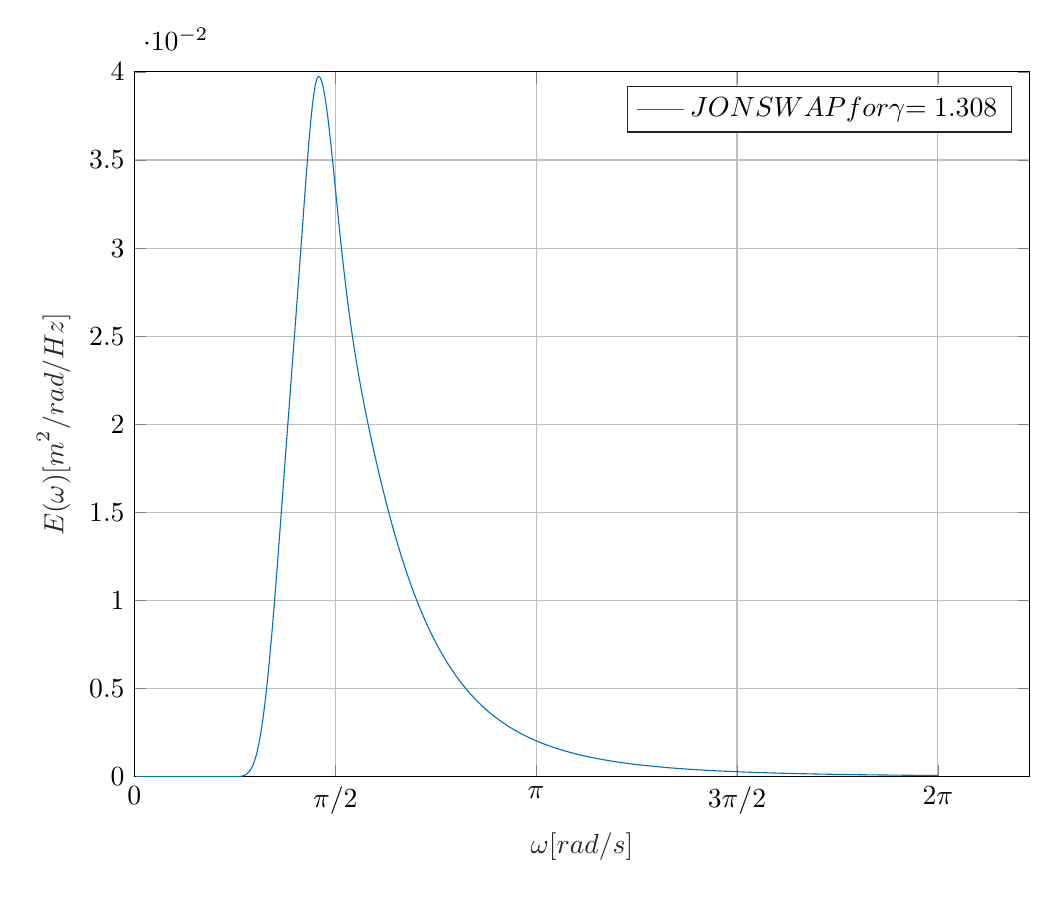
\begin{tikzpicture}

\begin{axis}[%
width=4.476in,
height=3.524in,
at={(0.803in,0.523in)},
scale only axis,
unbounded coords=jump,
xmin=0,
xmax=7,
xtick={0,1.5707963267949,3.14159265358979,4.71238898038469,6.28318530717959},
xticklabels={{0},{$\pi\text{/2}$},{$\pi$},{$\text{3}\pi\text{/2}$},{$\text{2}\pi$}},
xlabel style={font=\color{white!15!black}},
xlabel={$\omega\text{ [rad/s]}$},
ymin=0,
ymax=0.04,
ylabel style={font=\color{white!15!black}},
ylabel={$\text{E(}\omega\text{) [m}^\text{2}\text{/rad/Hz]}$},
axis background/.style={fill=white},
title style={font=\bfseries},
%title={$\text{One-dimensional wave spectrum, E(}\omega\text{) at -34S, 17.25E}$},
xmajorgrids,
ymajorgrids,
legend style={legend cell align=left, align=left, draw=white!15!black}
]
\addplot [color=mycolor1]
  table[row sep=crcr]{%
0	nan\\
0.0122958616578857	0\\
0.0245917233157714	0\\
0.0368875849736571	0\\
0.0491834466315427	0\\
0.0614793082894284	0\\
0.0737751699473141	0\\
0.0860710316051998	0\\
0.0983668932630855	0\\
0.110662754920971	0\\
0.122958616578857	0\\
0.135254478236743	0\\
0.147550339894628	0\\
0.159846201552514	0\\
0.1721420632104	0\\
0.184437924868285	0\\
0.196733786526171	0\\
0.209029648184057	0\\
0.221325509841942	0\\
0.233621371499828	0\\
0.245917233157714	0\\
0.258213094815599	0\\
0.270508956473485	0\\
0.282804818131371	0\\
0.295100679789256	5.41302879763333e-307\\
0.307396541447142	1.4351658983951e-260\\
0.319692403105028	1.39801651640755e-222\\
0.331988264762914	2.95955173493782e-191\\
0.344284126420799	3.06617261869068e-165\\
0.356579988078685	1.71585454184354e-143\\
0.368875849736571	3.36115162791715e-125\\
0.381171711394456	9.99471845091621e-110\\
0.393467573052342	1.44074967318733e-96\\
0.405763434710228	2.54134308132756e-85\\
0.418059296368113	1.15384979645612e-75\\
0.430355158025999	2.46010694641464e-67\\
0.442651019683885	4.01707121559874e-60\\
0.45494688134177	7.49671131280128e-54\\
0.467242742999656	2.22288404307939e-48\\
0.479538604657542	1.3753760835859e-43\\
0.491834466315427	2.22745866619101e-39\\
0.504130327973313	1.14105811314078e-35\\
0.516426189631199	2.16730148431401e-32\\
0.528722051289085	1.74501685936915e-29\\
0.54101791294697	6.67054290550385e-27\\
0.553313774604856	1.33294088654399e-24\\
0.565609636262742	1.51145852287043e-22\\
0.577905497920627	1.0433270916913e-20\\
0.590201359578513	4.65664898554377e-19\\
0.602497221236399	1.41551545559892e-17\\
0.614793082894284	3.06504085545376e-16\\
0.62708894455217	4.91508596715723e-15\\
0.639384806210056	6.03782647089776e-14\\
0.651680667867941	5.85166582657271e-13\\
0.663976529525827	4.59100381164424e-12\\
0.676272391183713	2.98235025750544e-11\\
0.688568252841599	1.63618607596188e-10\\
0.700864114499484	7.71435740175365e-10\\
0.71315997615737	3.17422780050511e-09\\
0.725455837815256	1.15545266932238e-08\\
0.737751699473141	3.76593918002615e-08\\
0.750047561131027	1.11082567474578e-07\\
0.762343422788913	2.99365257438456e-07\\
0.774639284446798	7.43398794457705e-07\\
0.786935146104684	1.71393732492197e-06\\
0.79923100776257	3.6936978163335e-06\\
0.811526869420455	7.48610717182671e-06\\
0.823822731078341	1.43464290828625e-05\\
0.836118592736227	2.61246562604755e-05\\
0.848414454394112	4.54036148623333e-05\\
0.860710316051998	7.56117606150625e-05\\
0.873006177709884	0.000121089372916668\\
0.88530203936777	0.000187089786772187\\
0.897597901025655	0.000279703606526386\\
0.909893762683541	0.000405702450085907\\
0.922189624341426	0.000572308176547121\\
0.934485485999312	0.000786902195884214\\
0.946781347657198	0.00105669606424971\\
0.959077209315084	0.00138838834019309\\
0.971373070972969	0.00178783338397504\\
0.983668932630855	0.00225974569705202\\
0.995964794288741	0.00280745915996462\\
1.00826065594663	0.00343275496464683\\
1.02055651760451	0.00413576600873186\\
1.0328523792624	0.00491495977802167\\
1.04514824092028	0.00576719685342651\\
1.05744410257817	0.00668785847600663\\
1.06973996423605	0.00767103419145496\\
1.08203582589394	0.00870975936699404\\
1.09433168755183	0.0097962920536587\\
1.10662754920971	0.0109224188636112\\
1.1189234108676	0.0120797798007726\\
1.13121927252548	0.0132602018978306\\
1.14351513418337	0.0144560307440969\\
1.15581099584125	0.0156604473784329\\
1.16810685749914	0.0168677556407375\\
1.18040271915703	0.0180736222488931\\
1.19269858081491	0.0192752491472963\\
1.2049944424728	0.0204714557558278\\
1.21729030413068	0.0216626483564445\\
1.22958616578857	0.0228506556097147\\
1.24188202744645	0.0240384135360737\\
1.25417788910434	0.0252294904939306\\
1.26647375076223	0.0264274529344006\\
1.27876961242011	0.0276350862726403\\
1.291065474078	0.0288535024756524\\
1.30336133573588	0.0300811872588852\\
1.31565719739377	0.0313130648442189\\
1.32795305905165	0.0325396852882558\\
1.34024892070954	0.0337466641153829\\
1.35254478236743	0.0349145188355605\\
1.36484064402531	0.0360190415875961\\
1.3771365056832	0.0370323108877261\\
1.38943236734108	0.0379243714742074\\
1.40172822899897	0.0386655021114703\\
1.41402409065685	0.0392288631897149\\
1.42631995231474	0.0395931988386078\\
1.43861581397263	0.0397451987880671\\
1.45091167563051	0.0397009837064543\\
1.4632075372884	0.0395060933162202\\
1.47550339894628	0.0391703952648501\\
1.48779926060417	0.0387059506556059\\
1.50009512226205	0.0381276193041899\\
1.51239098391994	0.0374522472133023\\
1.52468684557783	0.0366977905296433\\
1.53698270723571	0.0358824534634019\\
1.5492785688936	0.0350239067515314\\
1.56157443055148	0.0341386357865274\\
1.57387029220937	0.033241447182027\\
1.58616615386725	0.0323451427488864\\
1.59846201552514	0.0314603532066003\\
1.61075787718303	0.0305955119179262\\
1.62305373884091	0.0297569418708591\\
1.6353496004988	0.0289490265523619\\
1.64764546215668	0.0281744362672717\\
1.65994132381457	0.0274343846835443\\
1.67223718547245	0.0267288948374096\\
1.68453304713034	0.0260570586376697\\
1.69682890878822	0.0254172784703886\\
1.70912477044611	0.0248074834845985\\
1.721420632104	0.024225316400738\\
1.73371649376188	0.023668289227364\\
1.74601235541977	0.0231339081746281\\
1.75830821707765	0.0226197694201764\\
1.77060407873554	0.0221236283185714\\
1.78289994039342	0.0216434452374737\\
1.79519580205131	0.0211774115218765\\
1.8074916637092	0.0207239591846428\\
1.81978752536708	0.0202817578397189\\
1.83208338702497	0.0198497021705522\\
1.84437924868285	0.0194268928954684\\
1.85667511034074	0.0190126137886203\\
1.86897097199862	0.0186063068732881\\
1.88126683365651	0.0182075474549375\\
1.8935626953144	0.0178160202313337\\
1.90585855697228	0.0174314973270267\\
1.91815441863017	0.0170538187637728\\
1.93045028028805	0.0166828756042898\\
1.94274614194594	0.0163185957954444\\
1.95504200360382	0.0159609325850235\\
1.96733786526171	0.0156098552867384\\
1.9796337269196	0.015265342112225\\
1.99192958857748	0.0149273747670556\\
2.00422545023537	0.0145959345109985\\
2.01652131189325	0.0142709994027779\\
2.02881717355114	0.0139525424796016\\
2.04111303520902	0.0136405306563983\\
2.05340889686691	0.0133349241651845\\
2.0657047585248	0.0130356763886258\\
2.07800062018268	0.0127427339721329\\
2.09029648184057	0.0124560371249502\\
2.10259234349845	0.0121755200424896\\
2.11488820515634	0.0119011113998192\\
2.12718406681422	0.0116327348801607\\
2.13947992847211	0.011370309712995\\
2.15177579012999	0.0111137512044894\\
2.16407165178788	0.0108629712489418\\
2.17636751344577	0.0106178788142673\\
2.18866337510365	0.0103783803976124\\
2.20095923676154	0.0101443804493013\\
2.21325509841942	0.00991578176473845\\
2.22555096007731	0.00969248584482827\\
2.2378468217352	0.00947439322604724\\
2.25014268339308	0.00926140378164897\\
2.26243854505097	0.0090534169956585\\
2.27473440670885	0.00885033221138453\\
2.28703026836674	0.00865204885617913\\
2.29932613002462	0.00845846664413426\\
2.31162199168251	0.00826948575833719\\
2.3239178533404	0.00808500701422663\\
2.33621371499828	0.00790493200550391\\
2.34850957665617	0.00772916323396475\\
2.36080543831405	0.00755760422452847\\
2.37310129997194	0.00739015962665654\\
2.38539716162982	0.00722673530327022\\
2.39769302328771	0.00706723840819925\\
2.40998888494559	0.00691157745312068\\
2.42228474660348	0.0067596623648772\\
2.43458060826137	0.00661140453400037\\
2.44687646991925	0.00646671685520286\\
2.45917233157714	0.00632551376054758\\
2.47146819323502	0.00618771124594853\\
2.48376405489291	0.00605322689160874\\
2.49605991655079	0.00592197987695489\\
2.50835577820868	0.00579389099058502\\
2.52065163986657	0.00566888263570622\\
2.53294750152445	0.00554687883150177\\
2.54524336318234	0.00542780521083287\\
2.55753922484022	0.00531158901464808\\
2.56983508649811	0.00519815908344373\\
2.58213094815599	0.00508744584609102\\
2.59442680981388	0.00497938130631981\\
2.60672267147177	0.00487389902712567\\
2.61901853312965	0.00477093411334424\\
2.63131439478754	0.00467042319261705\\
2.64361025644542	0.00457230439495386\\
2.65590611810331	0.00447651733107909\\
2.66820197976119	0.00438300306973388\\
2.68049784141908	0.00429170411409041\\
2.69279370307697	0.00420256437742111\\
2.70508956473485	0.00411552915815301\\
2.71738542639274	0.00403054511442532\\
2.72968128805062	0.00394756023825787\\
2.74197714970851	0.00386652382942774\\
2.75427301136639	0.00378738646914243\\
2.76656887302428	0.00371009999358922\\
2.77886473468217	0.00363461746743274\\
2.79116059634005	0.00356089315732546\\
2.80345645799794	0.00348888250548924\\
2.81575231965582	0.00341854210342006\\
2.82804818131371	0.00334982966576232\\
2.84034404297159	0.00328270400439414\\
2.85263990462948	0.00321712500276036\\
2.86493576628737	0.00315305359048552\\
2.87723162794525	0.00309045171829528\\
2.88952748960314	0.00302928233327117\\
2.90182335126102	0.0029695093544601\\
2.91411921291891	0.00291109764885714\\
2.92641507457679	0.00285401300777748\\
2.93871093623468	0.00279822212363068\\
2.95100679789256	0.00274369256710825\\
2.96330265955045	0.00269039276479353\\
2.97559852120834	0.00263829197720089\\
2.98789438286622	0.00258736027724954\\
3.00019024452411	0.00253756852917576\\
3.01248610618199	0.00248888836788607\\
3.02478196783988	0.00244129217875227\\
3.03707782949776	0.00239475307784859\\
3.04937369115565	0.00234924489262979\\
3.06166955281354	0.0023047421430484\\
3.07396541447142	0.0022612200231083\\
3.08626127612931	0.00221865438285134\\
3.09855713778719	0.00217702171077273\\
3.11085299944508	0.00213629911666074\\
3.12314886110296	0.00209646431485547\\
3.13544472276085	0.00205749560792113\\
3.14774058441874	0.00201937187072593\\
3.16003644607662	0.00198207253492326\\
3.17233230773451	0.00194557757382764\\
3.18462816939239	0.00190986748767868\\
3.19692403105028	0.00187492328928602\\
3.20921989270816	0.00184072649004824\\
3.22151575436605	0.00180725908633834\\
3.23381161602394	0.00177450354624858\\
3.24610747768182	0.00174244279668723\\
3.25840333933971	0.00171106021081969\\
3.27069920099759	0.0016803395958467\\
3.28299506265548	0.00165026518111192\\
3.29529092431336	0.00162082160653164\\
3.30758678597125	0.00159199391133908\\
3.31988264762914	0.00156376752313587\\
3.33217850928702	0.00153612824724346\\
3.34447437094491	0.00150906225634721\\
3.35677023260279	0.00148255608042589\\
3.36906609426068	0.00145659659695957\\
3.38136195591856	0.00143117102140895\\
3.39365781757645	0.00140626689795909\\
3.40595367923434	0.00138187209052092\\
3.41824954089222	0.00135797477398379\\
3.43054540255011	0.00133456342571239\\
3.44284126420799	0.00131162681728186\\
3.45513712586588	0.00128915400644448\\
3.46743298752376	0.00126713432932197\\
3.47972884918165	0.00124555739281723\\
3.49202471083954	0.00122441306723957\\
3.50432057249742	0.00120369147913769\\
3.51661643415531	0.00118338300433464\\
3.52891229581319	0.00116347826115928\\
3.54120815747108	0.00114396810386871\\
3.55350401912896	0.00112484361625655\\
3.56579988078685	0.0011060961054416\\
3.57809574244473	0.00108771709583218\\
3.59039160410262	0.00106969832326091\\
3.60268746576051	0.00105203172928534\\
3.61498332741839	0.00103470945564963\\
3.62727918907628	0.0010177238389028\\
3.63957505073416	0.00100106740516895\\
3.65187091239205	0.000984732865065375\\
3.66416677404994	0.000968713108764074\\
3.67646263570782	0.00095300120119279\\
3.68875849736571	0.00093759037737141\\
3.70105435902359	0.000922474037879949\\
3.71335022068148	0.000907645744454282\\
3.72564608233936	0.000893099215705966\\
3.73794194399725	0.000878828322962575\\
3.75023780565513	0.000864827086225059\\
3.76253366731302	0.000851089670238769\\
3.77482952897091	0.000837610380674829\\
3.78712539062879	0.000824383660418703\\
3.79942125228668	0.000811404085962812\\
3.81171711394456	0.00079866636390022\\
3.82401297560245	0.000786165327516438\\
3.83630883726033	0.000773895933476511\\
3.84860469891822	0.000761853258604621\\
3.86090056057611	0.000750032496753526\\
3.87319642223399	0.000738428955761214\\
3.88549228389188	0.000727038054492271\\
3.89778814554976	0.000715855319961465\\
3.91008400720765	0.000704876384537197\\
3.92237986886553	0.000694096983222478\\
3.93467573052342	0.000683512951011199\\
3.94697159218131	0.000673120220317491\\
3.95926745383919	0.000662914818476088\\
3.97156331549708	0.000652892865311599\\
3.98385917715496	0.000643050570774724\\
3.99615503881285	0.000633384232643455\\
4.00845090047073	0.000623890234287399\\
4.02074676212862	0.000614565042493382\\
4.03304262378651	0.000605405205350579\\
4.04533848544439	0.000596407350193436\\
4.05763434710228	0.000587568181600735\\
4.06993020876016	0.000578884479449159\\
4.08222607041805	0.00057035309701982\\
4.09452193207593	0.000561970959156189\\
4.10681779373382	0.000553735060471986\\
4.1191136553917	0.000545642463607562\\
4.13140951704959	0.000537690297533413\\
4.14370537870748	0.00052987575589945\\
4.15600124036536	0.000522196095428724\\
4.16829710202325	0.000514648634354346\\
4.18059296368113	0.00050723075089834\\
4.19288882533902	0.00049993988179127\\
4.2051846869969	0.000492773520831441\\
4.21748054865479	0.00048572921748257\\
4.22977641031268	0.000478804575508837\\
4.24207227197056	0.000471997251646233\\
4.25436813362845	0.000465304954309197\\
4.26666399528633	0.000458725442331523\\
4.27895985694422	0.000452256523740597\\
4.29125571860211	0.000445896054563984\\
4.30355158025999	0.000439641937667487\\
4.31584744191788	0.000433492121623766\\
4.32814330357576	0.000427444599610678\\
4.34043916523365	0.000421497408338488\\
4.35273502689153	0.000415648627005148\\
4.36503088854942	0.000409896376278856\\
4.37732675020731	0.000404238817307136\\
4.38962261186519	0.000398674150751693\\
4.40191847352308	0.000393200615848326\\
4.41421433518096	0.000387816489491206\\
4.42651019683885	0.000382520085340833\\
4.43880605849673	0.000377309752955029\\
4.45110192015462	0.000372183876942308\\
4.46339778181251	0.000367140876137024\\
4.47569364347039	0.000362179202795692\\
4.48798950512828	0.000357297341813879\\
4.50028536678616	0.000352493809963128\\
4.51258122844405	0.000347767155147345\\
4.52487709010193	0.000343115955678117\\
4.53717295175982	0.000338538819568452\\
4.5494688134177	0.000334034383844427\\
4.56176467507559	0.000329601313874257\\
4.57406053673348	0.000325238302714321\\
4.58635639839136	0.000320944070471665\\
4.59865226004925	0.000316717363682552\\
4.61094812170713	0.000312556954706612\\
4.62324398336502	0.00030846164113618\\
4.6355398450229	0.000304430245220401\\
4.64783570668079	0.000300461613303707\\
4.66013156833868	0.000296554615278295\\
4.67242742999656	0.000292708144050196\\
4.68472329165445	0.000288921115018604\\
4.69701915331233	0.000285192465568094\\
4.70931501497022	0.000281521154573383\\
4.7216108766281	0.000277906161916305\\
4.73390673828599	0.000274346488014674\\
4.74620259994388	0.000270841153362717\\
4.75849846160176	0.000267389198082769\\
4.77079432325965	0.000263989681487935\\
4.78309018491753	0.000260641681655428\\
4.79538604657542	0.000257344295010299\\
4.8076819082333	0.000254096635919287\\
4.81997776989119	0.000250897836294526\\
4.83227363154908	0.000247747045206839\\
4.84456949320696	0.000244643428508389\\
4.85686535486485	0.000241586168464416\\
4.86916121652273	0.000238574463393844\\
4.88145707818062	0.000235607527318515\\
4.8937529398385	0.000232684589620834\\
4.90604880149639	0.000229804894709597\\
4.91834466315427	0.000226967701693801\\
4.93064052481216	0.000224172284064218\\
4.94293638647005	0.000221417929382543\\
4.95523224812793	0.000218703938977918\\
4.96752810978582	0.000216029627650631\\
4.9798239714437	0.000213394323382829\\
4.99211983310159	0.000210797367056043\\
5.00441569475948	0.000208238112175362\\
5.01671155641736	0.000205715924600084\\
5.02900741807525	0.000203230182280682\\
5.04130327973313	0.000200780275001916\\
5.05359914139102	0.000198365604131947\\
5.0658950030489	0.000195985582377289\\
5.07819086470679	0.00019363963354346\\
5.09048672636467	0.000191327192301187\\
5.10278258802256	0.000189047703958018\\
5.11507844968045	0.000186800624235214\\
5.12737431133833	0.00018458541904979\\
5.13967017299622	0.000182401564301559\\
5.1519660346541	0.000180248545665076\\
5.16426189631199	0.000178125858386348\\
5.17655775796987	0.000176033007084189\\
5.18885361962776	0.000173969505556115\\
5.20114948128565	0.000171934876588657\\
5.21344534294353	0.000169928651771981\\
5.22574120460142	0.000167950371318724\\
5.2380370662593	0.000165999583886923\\
5.25033292791719	0.000164075846406948\\
5.26262878957507	0.000162178723912337\\
5.27492465123296	0.000160307789374435\\
5.28722051289085	0.000158462623540752\\
5.29951637454873	0.000156642814776941\\
5.31181223620662	0.000154847958912307\\
5.3241080978645	0.000153077659088771\\
5.33640395952239	0.000151331525613192\\
5.34869982118027	0.000149609175812981\\
5.36099568283816	0.000147910233894908\\
5.37329154449605	0.000146234330807043\\
5.38558740615393	0.000144581104103749\\
5.39788326781182	0.000142950197813643\\
5.4101791294697	0.000141341262310475\\
5.42247499112759	0.000139753954186838\\
5.43477085278547	0.000138187936130644\\
5.44706671444336	0.000136642876804307\\
5.45936257610125	0.000135118450726565\\
5.47165843775913	0.000133614338156872\\
5.48395429941702	0.00013213022498231\\
5.4962501610749	0.00013066580260695\\
5.50854602273279	0.000129220767843618\\
5.52084188439067	0.000127794822807993\\
5.53313774604856	0.000126387674814993\\
5.54543360770645	0.000124999036277395\\
5.55772946936433	0.000123628624606628\\
5.57002533102222	0.000122276162115703\\
5.5823211926801	0.00012094137592421\\
5.59461705433799	0.000119623997865353\\
5.60691291599587	0.000118323764394966\\
5.61920877765376	0.00011704041650246\\
5.63150463931164	0.000115773699623671\\
5.64380050096953	0.000114523363555545\\
5.65609636262742	0.000113289162372638\\
5.6683922242853	0.00011207085434537\\
5.68068808594319	0.000110868201860007\\
5.69298394760107	0.000109680971340328\\
5.70527980925896	0.00010850893317093\\
5.71757567091684	0.000107351861622146\\
5.72987153257473	0.000106209534776526\\
5.74216739423262	0.000105081734456864\\
5.7544632558905	0.000103968246155711\\
5.76675911754839	0.000102868858966361\\
5.77905497920627	0.000101783365515268\\
5.79135084086416	0.000100711561895862\\
5.80364670252204	9.96532476037344e-05\\
5.81594256417993	9.86082254731543e-05\\
5.82823842583782	9.75763016149018e-05\\
5.8405342874957	9.65572853553714e-05\\
5.85283014915359	9.55509891769276e-05\\
5.86512601081147	9.455722865948e-05\\
5.87742187246936	9.35758224232536e-05\\
5.88971773412724	9.26065920727251e-05\\
5.90201359578513	9.16493621417014e-05\\
5.91430945744302	9.07039600395125e-05\\
5.9266053191009	8.97702159982964e-05\\
5.93890118075879	8.88479630213512e-05\\
5.95119704241667	8.79370368325295e-05\\
5.96349290407456	8.70372758266536e-05\\
5.97578876573244	8.61485210209284e-05\\
5.98808462739033	8.5270616007331e-05\\
6.00038048904822	8.4403406905953e-05\\
6.0126763507061	8.35467423192785e-05\\
6.02497221236399	8.27004732873734e-05\\
6.03726807402187	8.18644532439695e-05\\
6.04956393567976	8.10385379734214e-05\\
6.06185979733764	8.02225855685183e-05\\
6.07415565899553	7.94164563891332e-05\\
6.08645152065342	7.86200130216882e-05\\
6.0987473823113	7.78331202394225e-05\\
6.11104324396919	7.70556449634419e-05\\
6.12333910562707	7.62874562245356e-05\\
6.13563496728496	7.55284251257423e-05\\
6.14793082894284	7.4778424805651e-05\\
6.16022669060073	7.40373304024179e-05\\
6.17252255225862	7.33050190184887e-05\\
6.1848184139165	7.25813696860062e-05\\
6.19711427557439	7.18662633328921e-05\\
6.20941013723227	7.11595827495877e-05\\
6.22170599889016	7.04612125564384e-05\\
6.23400186054804	6.97710391717103e-05\\
6.24629772220593	6.90889507802242e-05\\
6.25859358386381	6.84148373025936e-05\\
6.2708894455217	6.77485903650559e-05\\
6.28318530717959	6.70901032698821e-05\\
};
\addlegendentry{$\text{JONSWAP for }\gamma\text{ = 1.308}$}

\end{axis}
\end{tikzpicture}%}
    }
    \subcaptionbox{\acs{jonswap} spectrum at multiple geographical locations\label{fig:systemDesign.1DSampleWaveSpectrumMultiple}}[0.48\linewidth]{
        \resizebox{\linewidth}{!}{% This file was created by matlab2tikz.
%
%The latest updates can be retrieved from
%  http://www.mathworks.com/matlabcentral/fileexchange/22022-matlab2tikz-matlab2tikz
%where you can also make suggestions and rate matlab2tikz.
%
\definecolor{mycolor1}{rgb}{0.00000,0.44700,0.74100}%
\definecolor{mycolor2}{rgb}{0.85000,0.32500,0.09800}%
\definecolor{mycolor3}{rgb}{0.92900,0.69400,0.12500}%
%
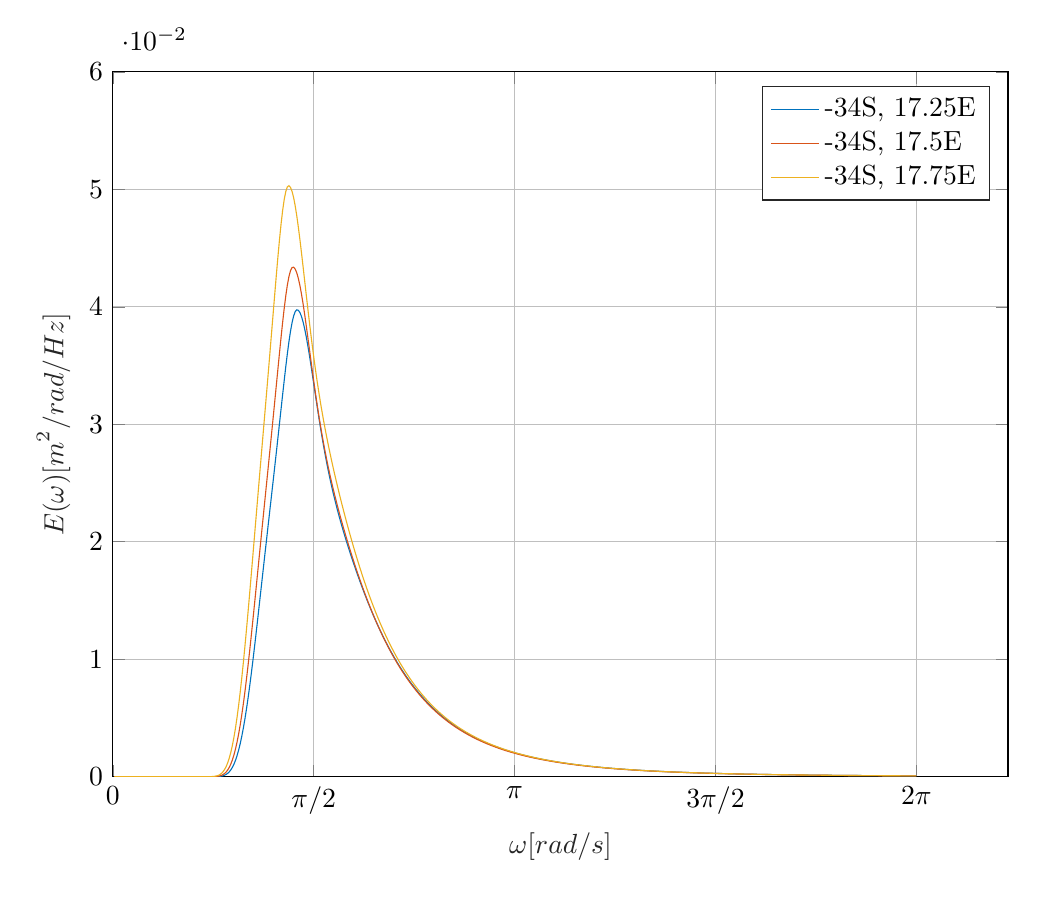
\begin{tikzpicture}

\begin{axis}[%
width=4.476in,
height=3.524in,
at={(0.803in,0.523in)},
scale only axis,
unbounded coords=jump,
xmin=0,
xmax=7,
xtick={0,1.5707963267949,3.14159265358979,4.71238898038469,6.28318530717959},
xticklabels={{0},{$\pi\text{/2}$},{$\pi$},{$\text{3}\pi\text{/2}$},{$\text{2}\pi$}},
xlabel style={font=\color{white!15!black}},
xlabel={$\omega\text{ [rad/s]}$},
ymin=0,
ymax=0.06,
ylabel style={font=\color{white!15!black}},
ylabel={$\text{E(}\omega\text{) [m}^\text{2}\text{/rad/Hz]}$},
axis background/.style={fill=white},
title style={font=\bfseries},
xmajorgrids,
ymajorgrids,
legend style={legend cell align=left, align=left, draw=white!15!black}
]
\addplot [color=mycolor1]
  table[row sep=crcr]{%
0	nan\\
0.0122958616578857	0\\
0.0245917233157714	0\\
0.0368875849736571	0\\
0.0491834466315427	0\\
0.0614793082894284	0\\
0.0737751699473141	0\\
0.0860710316051998	0\\
0.0983668932630855	0\\
0.110662754920971	0\\
0.122958616578857	0\\
0.135254478236743	0\\
0.147550339894628	0\\
0.159846201552514	0\\
0.1721420632104	0\\
0.184437924868285	0\\
0.196733786526171	0\\
0.209029648184057	0\\
0.221325509841942	0\\
0.233621371499828	0\\
0.245917233157714	0\\
0.258213094815599	0\\
0.270508956473485	0\\
0.282804818131371	0\\
0.295100679789256	5.41302879763333e-307\\
0.307396541447142	1.4351658983951e-260\\
0.319692403105028	1.39801651640755e-222\\
0.331988264762914	2.95955173493782e-191\\
0.344284126420799	3.06617261869068e-165\\
0.356579988078685	1.71585454184354e-143\\
0.368875849736571	3.36115162791715e-125\\
0.381171711394456	9.99471845091621e-110\\
0.393467573052342	1.44074967318733e-96\\
0.405763434710228	2.54134308132756e-85\\
0.418059296368113	1.15384979645612e-75\\
0.430355158025999	2.46010694641464e-67\\
0.442651019683885	4.01707121559874e-60\\
0.45494688134177	7.49671131280128e-54\\
0.467242742999656	2.22288404307939e-48\\
0.479538604657542	1.3753760835859e-43\\
0.491834466315427	2.22745866619101e-39\\
0.504130327973313	1.14105811314078e-35\\
0.516426189631199	2.16730148431401e-32\\
0.528722051289085	1.74501685936915e-29\\
0.54101791294697	6.67054290550385e-27\\
0.553313774604856	1.33294088654399e-24\\
0.565609636262742	1.51145852287043e-22\\
0.577905497920627	1.0433270916913e-20\\
0.590201359578513	4.65664898554377e-19\\
0.602497221236399	1.41551545559892e-17\\
0.614793082894284	3.06504085545376e-16\\
0.62708894455217	4.91508596715723e-15\\
0.639384806210056	6.03782647089776e-14\\
0.651680667867941	5.85166582657271e-13\\
0.663976529525827	4.59100381164424e-12\\
0.676272391183713	2.98235025750544e-11\\
0.688568252841599	1.63618607596188e-10\\
0.700864114499484	7.71435740175365e-10\\
0.71315997615737	3.17422780050511e-09\\
0.725455837815256	1.15545266932238e-08\\
0.737751699473141	3.76593918002615e-08\\
0.750047561131027	1.11082567474578e-07\\
0.762343422788913	2.99365257438456e-07\\
0.774639284446798	7.43398794457705e-07\\
0.786935146104684	1.71393732492197e-06\\
0.79923100776257	3.6936978163335e-06\\
0.811526869420455	7.48610717182671e-06\\
0.823822731078341	1.43464290828625e-05\\
0.836118592736227	2.61246562604755e-05\\
0.848414454394112	4.54036148623333e-05\\
0.860710316051998	7.56117606150625e-05\\
0.873006177709884	0.000121089372916668\\
0.88530203936777	0.000187089786772187\\
0.897597901025655	0.000279703606526386\\
0.909893762683541	0.000405702450085907\\
0.922189624341426	0.000572308176547121\\
0.934485485999312	0.000786902195884214\\
0.946781347657198	0.00105669606424971\\
0.959077209315084	0.00138838834019309\\
0.971373070972969	0.00178783338397504\\
0.983668932630855	0.00225974569705202\\
0.995964794288741	0.00280745915996462\\
1.00826065594663	0.00343275496464683\\
1.02055651760451	0.00413576600873186\\
1.0328523792624	0.00491495977802167\\
1.04514824092028	0.00576719685342651\\
1.05744410257817	0.00668785847600663\\
1.06973996423605	0.00767103419145496\\
1.08203582589394	0.00870975936699404\\
1.09433168755183	0.0097962920536587\\
1.10662754920971	0.0109224188636112\\
1.1189234108676	0.0120797798007726\\
1.13121927252548	0.0132602018978306\\
1.14351513418337	0.0144560307440969\\
1.15581099584125	0.0156604473784329\\
1.16810685749914	0.0168677556407375\\
1.18040271915703	0.0180736222488931\\
1.19269858081491	0.0192752491472963\\
1.2049944424728	0.0204714557558278\\
1.21729030413068	0.0216626483564445\\
1.22958616578857	0.0228506556097147\\
1.24188202744645	0.0240384135360737\\
1.25417788910434	0.0252294904939306\\
1.26647375076223	0.0264274529344006\\
1.27876961242011	0.0276350862726403\\
1.291065474078	0.0288535024756524\\
1.30336133573588	0.0300811872588852\\
1.31565719739377	0.0313130648442189\\
1.32795305905165	0.0325396852882558\\
1.34024892070954	0.0337466641153829\\
1.35254478236743	0.0349145188355605\\
1.36484064402531	0.0360190415875961\\
1.3771365056832	0.0370323108877261\\
1.38943236734108	0.0379243714742074\\
1.40172822899897	0.0386655021114703\\
1.41402409065685	0.0392288631897149\\
1.42631995231474	0.0395931988386078\\
1.43861581397263	0.0397451987880671\\
1.45091167563051	0.0397009837064543\\
1.4632075372884	0.0395060933162202\\
1.47550339894628	0.0391703952648501\\
1.48779926060417	0.0387059506556059\\
1.50009512226205	0.0381276193041899\\
1.51239098391994	0.0374522472133023\\
1.52468684557783	0.0366977905296433\\
1.53698270723571	0.0358824534634019\\
1.5492785688936	0.0350239067515314\\
1.56157443055148	0.0341386357865274\\
1.57387029220937	0.033241447182027\\
1.58616615386725	0.0323451427488864\\
1.59846201552514	0.0314603532066003\\
1.61075787718303	0.0305955119179262\\
1.62305373884091	0.0297569418708591\\
1.6353496004988	0.0289490265523619\\
1.64764546215668	0.0281744362672717\\
1.65994132381457	0.0274343846835443\\
1.67223718547245	0.0267288948374096\\
1.68453304713034	0.0260570586376697\\
1.69682890878822	0.0254172784703886\\
1.70912477044611	0.0248074834845985\\
1.721420632104	0.024225316400738\\
1.73371649376188	0.023668289227364\\
1.74601235541977	0.0231339081746281\\
1.75830821707765	0.0226197694201764\\
1.77060407873554	0.0221236283185714\\
1.78289994039342	0.0216434452374737\\
1.79519580205131	0.0211774115218765\\
1.8074916637092	0.0207239591846428\\
1.81978752536708	0.0202817578397189\\
1.83208338702497	0.0198497021705522\\
1.84437924868285	0.0194268928954684\\
1.85667511034074	0.0190126137886203\\
1.86897097199862	0.0186063068732881\\
1.88126683365651	0.0182075474549375\\
1.8935626953144	0.0178160202313337\\
1.90585855697228	0.0174314973270267\\
1.91815441863017	0.0170538187637728\\
1.93045028028805	0.0166828756042898\\
1.94274614194594	0.0163185957954444\\
1.95504200360382	0.0159609325850235\\
1.96733786526171	0.0156098552867384\\
1.9796337269196	0.015265342112225\\
1.99192958857748	0.0149273747670556\\
2.00422545023537	0.0145959345109985\\
2.01652131189325	0.0142709994027779\\
2.02881717355114	0.0139525424796016\\
2.04111303520902	0.0136405306563983\\
2.05340889686691	0.0133349241651845\\
2.0657047585248	0.0130356763886258\\
2.07800062018268	0.0127427339721329\\
2.09029648184057	0.0124560371249502\\
2.10259234349845	0.0121755200424896\\
2.11488820515634	0.0119011113998192\\
2.12718406681422	0.0116327348801607\\
2.13947992847211	0.011370309712995\\
2.15177579012999	0.0111137512044894\\
2.16407165178788	0.0108629712489418\\
2.17636751344577	0.0106178788142673\\
2.18866337510365	0.0103783803976124\\
2.20095923676154	0.0101443804493013\\
2.21325509841942	0.00991578176473845\\
2.22555096007731	0.00969248584482827\\
2.2378468217352	0.00947439322604724\\
2.25014268339308	0.00926140378164897\\
2.26243854505097	0.0090534169956585\\
2.27473440670885	0.00885033221138453\\
2.28703026836674	0.00865204885617913\\
2.29932613002462	0.00845846664413426\\
2.31162199168251	0.00826948575833719\\
2.3239178533404	0.00808500701422663\\
2.33621371499828	0.00790493200550391\\
2.34850957665617	0.00772916323396475\\
2.36080543831405	0.00755760422452847\\
2.37310129997194	0.00739015962665654\\
2.38539716162982	0.00722673530327022\\
2.39769302328771	0.00706723840819925\\
2.40998888494559	0.00691157745312068\\
2.42228474660348	0.0067596623648772\\
2.43458060826137	0.00661140453400037\\
2.44687646991925	0.00646671685520286\\
2.45917233157714	0.00632551376054758\\
2.47146819323502	0.00618771124594853\\
2.48376405489291	0.00605322689160874\\
2.49605991655079	0.00592197987695489\\
2.50835577820868	0.00579389099058502\\
2.52065163986657	0.00566888263570622\\
2.53294750152445	0.00554687883150177\\
2.54524336318234	0.00542780521083287\\
2.55753922484022	0.00531158901464808\\
2.56983508649811	0.00519815908344373\\
2.58213094815599	0.00508744584609102\\
2.59442680981388	0.00497938130631981\\
2.60672267147177	0.00487389902712567\\
2.61901853312965	0.00477093411334424\\
2.63131439478754	0.00467042319261705\\
2.64361025644542	0.00457230439495386\\
2.65590611810331	0.00447651733107909\\
2.66820197976119	0.00438300306973388\\
2.68049784141908	0.00429170411409041\\
2.69279370307697	0.00420256437742111\\
2.70508956473485	0.00411552915815301\\
2.71738542639274	0.00403054511442532\\
2.72968128805062	0.00394756023825787\\
2.74197714970851	0.00386652382942774\\
2.75427301136639	0.00378738646914243\\
2.76656887302428	0.00371009999358922\\
2.77886473468217	0.00363461746743274\\
2.79116059634005	0.00356089315732546\\
2.80345645799794	0.00348888250548924\\
2.81575231965582	0.00341854210342006\\
2.82804818131371	0.00334982966576232\\
2.84034404297159	0.00328270400439414\\
2.85263990462948	0.00321712500276036\\
2.86493576628737	0.00315305359048552\\
2.87723162794525	0.00309045171829528\\
2.88952748960314	0.00302928233327117\\
2.90182335126102	0.0029695093544601\\
2.91411921291891	0.00291109764885714\\
2.92641507457679	0.00285401300777748\\
2.93871093623468	0.00279822212363068\\
2.95100679789256	0.00274369256710825\\
2.96330265955045	0.00269039276479353\\
2.97559852120834	0.00263829197720089\\
2.98789438286622	0.00258736027724954\\
3.00019024452411	0.00253756852917576\\
3.01248610618199	0.00248888836788607\\
3.02478196783988	0.00244129217875227\\
3.03707782949776	0.00239475307784859\\
3.04937369115565	0.00234924489262979\\
3.06166955281354	0.0023047421430484\\
3.07396541447142	0.0022612200231083\\
3.08626127612931	0.00221865438285134\\
3.09855713778719	0.00217702171077273\\
3.11085299944508	0.00213629911666074\\
3.12314886110296	0.00209646431485547\\
3.13544472276085	0.00205749560792113\\
3.14774058441874	0.00201937187072593\\
3.16003644607662	0.00198207253492326\\
3.17233230773451	0.00194557757382764\\
3.18462816939239	0.00190986748767868\\
3.19692403105028	0.00187492328928602\\
3.20921989270816	0.00184072649004824\\
3.22151575436605	0.00180725908633834\\
3.23381161602394	0.00177450354624858\\
3.24610747768182	0.00174244279668723\\
3.25840333933971	0.00171106021081969\\
3.27069920099759	0.0016803395958467\\
3.28299506265548	0.00165026518111192\\
3.29529092431336	0.00162082160653164\\
3.30758678597125	0.00159199391133908\\
3.31988264762914	0.00156376752313587\\
3.33217850928702	0.00153612824724346\\
3.34447437094491	0.00150906225634721\\
3.35677023260279	0.00148255608042589\\
3.36906609426068	0.00145659659695957\\
3.38136195591856	0.00143117102140895\\
3.39365781757645	0.00140626689795909\\
3.40595367923434	0.00138187209052092\\
3.41824954089222	0.00135797477398379\\
3.43054540255011	0.00133456342571239\\
3.44284126420799	0.00131162681728186\\
3.45513712586588	0.00128915400644448\\
3.46743298752376	0.00126713432932197\\
3.47972884918165	0.00124555739281723\\
3.49202471083954	0.00122441306723957\\
3.50432057249742	0.00120369147913769\\
3.51661643415531	0.00118338300433464\\
3.52891229581319	0.00116347826115928\\
3.54120815747108	0.00114396810386871\\
3.55350401912896	0.00112484361625655\\
3.56579988078685	0.0011060961054416\\
3.57809574244473	0.00108771709583218\\
3.59039160410262	0.00106969832326091\\
3.60268746576051	0.00105203172928534\\
3.61498332741839	0.00103470945564963\\
3.62727918907628	0.0010177238389028\\
3.63957505073416	0.00100106740516895\\
3.65187091239205	0.000984732865065375\\
3.66416677404994	0.000968713108764074\\
3.67646263570782	0.00095300120119279\\
3.68875849736571	0.00093759037737141\\
3.70105435902359	0.000922474037879949\\
3.71335022068148	0.000907645744454282\\
3.72564608233936	0.000893099215705966\\
3.73794194399725	0.000878828322962575\\
3.75023780565513	0.000864827086225059\\
3.76253366731302	0.000851089670238769\\
3.77482952897091	0.000837610380674829\\
3.78712539062879	0.000824383660418703\\
3.79942125228668	0.000811404085962812\\
3.81171711394456	0.00079866636390022\\
3.82401297560245	0.000786165327516438\\
3.83630883726033	0.000773895933476511\\
3.84860469891822	0.000761853258604621\\
3.86090056057611	0.000750032496753526\\
3.87319642223399	0.000738428955761214\\
3.88549228389188	0.000727038054492271\\
3.89778814554976	0.000715855319961465\\
3.91008400720765	0.000704876384537197\\
3.92237986886553	0.000694096983222478\\
3.93467573052342	0.000683512951011199\\
3.94697159218131	0.000673120220317491\\
3.95926745383919	0.000662914818476088\\
3.97156331549708	0.000652892865311599\\
3.98385917715496	0.000643050570774724\\
3.99615503881285	0.000633384232643455\\
4.00845090047073	0.000623890234287399\\
4.02074676212862	0.000614565042493382\\
4.03304262378651	0.000605405205350579\\
4.04533848544439	0.000596407350193436\\
4.05763434710228	0.000587568181600735\\
4.06993020876016	0.000578884479449159\\
4.08222607041805	0.00057035309701982\\
4.09452193207593	0.000561970959156189\\
4.10681779373382	0.000553735060471986\\
4.1191136553917	0.000545642463607562\\
4.13140951704959	0.000537690297533413\\
4.14370537870748	0.00052987575589945\\
4.15600124036536	0.000522196095428724\\
4.16829710202325	0.000514648634354346\\
4.18059296368113	0.00050723075089834\\
4.19288882533902	0.00049993988179127\\
4.2051846869969	0.000492773520831441\\
4.21748054865479	0.00048572921748257\\
4.22977641031268	0.000478804575508837\\
4.24207227197056	0.000471997251646233\\
4.25436813362845	0.000465304954309197\\
4.26666399528633	0.000458725442331523\\
4.27895985694422	0.000452256523740597\\
4.29125571860211	0.000445896054563984\\
4.30355158025999	0.000439641937667487\\
4.31584744191788	0.000433492121623766\\
4.32814330357576	0.000427444599610678\\
4.34043916523365	0.000421497408338488\\
4.35273502689153	0.000415648627005148\\
4.36503088854942	0.000409896376278856\\
4.37732675020731	0.000404238817307136\\
4.38962261186519	0.000398674150751693\\
4.40191847352308	0.000393200615848326\\
4.41421433518096	0.000387816489491206\\
4.42651019683885	0.000382520085340833\\
4.43880605849673	0.000377309752955029\\
4.45110192015462	0.000372183876942308\\
4.46339778181251	0.000367140876137024\\
4.47569364347039	0.000362179202795692\\
4.48798950512828	0.000357297341813879\\
4.50028536678616	0.000352493809963128\\
4.51258122844405	0.000347767155147345\\
4.52487709010193	0.000343115955678117\\
4.53717295175982	0.000338538819568452\\
4.5494688134177	0.000334034383844427\\
4.56176467507559	0.000329601313874257\\
4.57406053673348	0.000325238302714321\\
4.58635639839136	0.000320944070471665\\
4.59865226004925	0.000316717363682552\\
4.61094812170713	0.000312556954706612\\
4.62324398336502	0.00030846164113618\\
4.6355398450229	0.000304430245220401\\
4.64783570668079	0.000300461613303707\\
4.66013156833868	0.000296554615278295\\
4.67242742999656	0.000292708144050196\\
4.68472329165445	0.000288921115018604\\
4.69701915331233	0.000285192465568094\\
4.70931501497022	0.000281521154573383\\
4.7216108766281	0.000277906161916305\\
4.73390673828599	0.000274346488014674\\
4.74620259994388	0.000270841153362717\\
4.75849846160176	0.000267389198082769\\
4.77079432325965	0.000263989681487935\\
4.78309018491753	0.000260641681655428\\
4.79538604657542	0.000257344295010299\\
4.8076819082333	0.000254096635919287\\
4.81997776989119	0.000250897836294526\\
4.83227363154908	0.000247747045206839\\
4.84456949320696	0.000244643428508389\\
4.85686535486485	0.000241586168464416\\
4.86916121652273	0.000238574463393844\\
4.88145707818062	0.000235607527318515\\
4.8937529398385	0.000232684589620834\\
4.90604880149639	0.000229804894709597\\
4.91834466315427	0.000226967701693801\\
4.93064052481216	0.000224172284064218\\
4.94293638647005	0.000221417929382543\\
4.95523224812793	0.000218703938977918\\
4.96752810978582	0.000216029627650631\\
4.9798239714437	0.000213394323382829\\
4.99211983310159	0.000210797367056043\\
5.00441569475948	0.000208238112175362\\
5.01671155641736	0.000205715924600084\\
5.02900741807525	0.000203230182280682\\
5.04130327973313	0.000200780275001916\\
5.05359914139102	0.000198365604131947\\
5.0658950030489	0.000195985582377289\\
5.07819086470679	0.00019363963354346\\
5.09048672636467	0.000191327192301187\\
5.10278258802256	0.000189047703958018\\
5.11507844968045	0.000186800624235214\\
5.12737431133833	0.00018458541904979\\
5.13967017299622	0.000182401564301559\\
5.1519660346541	0.000180248545665076\\
5.16426189631199	0.000178125858386348\\
5.17655775796987	0.000176033007084189\\
5.18885361962776	0.000173969505556115\\
5.20114948128565	0.000171934876588657\\
5.21344534294353	0.000169928651771981\\
5.22574120460142	0.000167950371318724\\
5.2380370662593	0.000165999583886923\\
5.25033292791719	0.000164075846406948\\
5.26262878957507	0.000162178723912337\\
5.27492465123296	0.000160307789374435\\
5.28722051289085	0.000158462623540752\\
5.29951637454873	0.000156642814776941\\
5.31181223620662	0.000154847958912307\\
5.3241080978645	0.000153077659088771\\
5.33640395952239	0.000151331525613192\\
5.34869982118027	0.000149609175812981\\
5.36099568283816	0.000147910233894908\\
5.37329154449605	0.000146234330807043\\
5.38558740615393	0.000144581104103749\\
5.39788326781182	0.000142950197813643\\
5.4101791294697	0.000141341262310475\\
5.42247499112759	0.000139753954186838\\
5.43477085278547	0.000138187936130644\\
5.44706671444336	0.000136642876804307\\
5.45936257610125	0.000135118450726565\\
5.47165843775913	0.000133614338156872\\
5.48395429941702	0.00013213022498231\\
5.4962501610749	0.00013066580260695\\
5.50854602273279	0.000129220767843618\\
5.52084188439067	0.000127794822807993\\
5.53313774604856	0.000126387674814993\\
5.54543360770645	0.000124999036277395\\
5.55772946936433	0.000123628624606628\\
5.57002533102222	0.000122276162115703\\
5.5823211926801	0.00012094137592421\\
5.59461705433799	0.000119623997865353\\
5.60691291599587	0.000118323764394966\\
5.61920877765376	0.00011704041650246\\
5.63150463931164	0.000115773699623671\\
5.64380050096953	0.000114523363555545\\
5.65609636262742	0.000113289162372638\\
5.6683922242853	0.00011207085434537\\
5.68068808594319	0.000110868201860007\\
5.69298394760107	0.000109680971340328\\
5.70527980925896	0.00010850893317093\\
5.71757567091684	0.000107351861622146\\
5.72987153257473	0.000106209534776526\\
5.74216739423262	0.000105081734456864\\
5.7544632558905	0.000103968246155711\\
5.76675911754839	0.000102868858966361\\
5.77905497920627	0.000101783365515268\\
5.79135084086416	0.000100711561895862\\
5.80364670252204	9.96532476037344e-05\\
5.81594256417993	9.86082254731543e-05\\
5.82823842583782	9.75763016149018e-05\\
5.8405342874957	9.65572853553714e-05\\
5.85283014915359	9.55509891769276e-05\\
5.86512601081147	9.455722865948e-05\\
5.87742187246936	9.35758224232536e-05\\
5.88971773412724	9.26065920727251e-05\\
5.90201359578513	9.16493621417014e-05\\
5.91430945744302	9.07039600395125e-05\\
5.9266053191009	8.97702159982964e-05\\
5.93890118075879	8.88479630213512e-05\\
5.95119704241667	8.79370368325295e-05\\
5.96349290407456	8.70372758266536e-05\\
5.97578876573244	8.61485210209284e-05\\
5.98808462739033	8.5270616007331e-05\\
6.00038048904822	8.4403406905953e-05\\
6.0126763507061	8.35467423192785e-05\\
6.02497221236399	8.27004732873734e-05\\
6.03726807402187	8.18644532439695e-05\\
6.04956393567976	8.10385379734214e-05\\
6.06185979733764	8.02225855685183e-05\\
6.07415565899553	7.94164563891332e-05\\
6.08645152065342	7.86200130216882e-05\\
6.0987473823113	7.78331202394225e-05\\
6.11104324396919	7.70556449634419e-05\\
6.12333910562707	7.62874562245356e-05\\
6.13563496728496	7.55284251257423e-05\\
6.14793082894284	7.4778424805651e-05\\
6.16022669060073	7.40373304024179e-05\\
6.17252255225862	7.33050190184887e-05\\
6.1848184139165	7.25813696860062e-05\\
6.19711427557439	7.18662633328921e-05\\
6.20941013723227	7.11595827495877e-05\\
6.22170599889016	7.04612125564384e-05\\
6.23400186054804	6.97710391717103e-05\\
6.24629772220593	6.90889507802242e-05\\
6.25859358386381	6.84148373025936e-05\\
6.2708894455217	6.77485903650559e-05\\
6.28318530717959	6.70901032698821e-05\\
};
\addlegendentry{-34S, 17.25E}

\addplot [color=mycolor2]
  table[row sep=crcr]{%
0	nan\\
0.0122958616578857	0\\
0.0245917233157714	0\\
0.0368875849736571	0\\
0.0491834466315427	0\\
0.0614793082894284	0\\
0.0737751699473141	0\\
0.0860710316051998	0\\
0.0983668932630855	0\\
0.110662754920971	0\\
0.122958616578857	0\\
0.135254478236743	0\\
0.147550339894628	0\\
0.159846201552514	0\\
0.1721420632104	0\\
0.184437924868285	0\\
0.196733786526171	0\\
0.209029648184057	0\\
0.221325509841942	0\\
0.233621371499828	0\\
0.245917233157714	0\\
0.258213094815599	0\\
0.270508956473485	0\\
0.282804818131371	0\\
0.295100679789256	3.11952792138373e-280\\
0.307396541447142	7.66084143312335e-238\\
0.319692403105028	3.72681629921495e-203\\
0.331988264762914	1.4912534528597e-174\\
0.344284126420799	8.43653670543348e-151\\
0.356579988078685	6.04760576222463e-131\\
0.368875849736571	3.02708863341633e-114\\
0.381171711394456	4.03994375317077e-100\\
0.393467573052342	4.15101868129121e-88\\
0.405763434710228	7.64896595290681e-78\\
0.418059296368113	4.98491809647189e-69\\
0.430355158025999	1.98964807806706e-61\\
0.442651019683885	7.60255241888616e-55\\
0.45494688134177	4.00846602943213e-49\\
0.467242742999656	3.94000605906152e-44\\
0.479538604657542	9.2601380862337e-40\\
0.491834466315427	6.4006391403998e-36\\
0.504130327973313	1.54669467365009e-32\\
0.516426189631199	1.51069034859478e-29\\
0.528722051289085	6.73973832524023e-27\\
0.54101791294697	1.52316693804866e-24\\
0.553313774604856	1.90399549411665e-22\\
0.565609636262742	1.41889521337791e-20\\
0.577905497920627	6.72132537416526e-19\\
0.590201359578513	2.1384287075339e-17\\
0.602497221236399	4.79147783814395e-16\\
0.614793082894284	7.87730943435279e-15\\
0.62708894455217	9.8456582169049e-14\\
0.639384806210056	9.64884816222262e-13\\
0.651680667867941	7.61644887696551e-12\\
0.663976529525827	4.95773990178333e-11\\
0.676272391183713	2.71650804509762e-10\\
0.688568252841599	1.27581119100493e-09\\
0.700864114499484	5.21820708795641e-09\\
0.71315997615737	1.88500613744762e-08\\
0.725455837815256	6.08907410251621e-08\\
0.737751699473141	1.77833102908609e-07\\
0.750047561131027	4.74172843633731e-07\\
0.762343422788913	1.16438052863903e-06\\
0.774639284446798	2.65368000406345e-06\\
0.786935146104684	5.65195325871851e-06\\
0.79923100776257	1.1319551048663e-05\\
0.811526869420455	2.14360862248871e-05\\
0.823822731078341	3.85749951386886e-05\\
0.836118592736227	6.6259876995127e-05\\
0.848414454394112	0.000109075349296092\\
0.860710316051998	0.000172706625403214\\
0.873006177709884	0.00026388833343557\\
0.88530203936777	0.000390253221673118\\
0.897597901025655	0.000560083487375966\\
0.909893762683541	0.000781979370649354\\
0.922189624341426	0.00106446942944156\\
0.934485485999312	0.00141559320318485\\
0.946781347657198	0.00184248919641237\\
0.959077209315084	0.00235101943210934\\
0.971373070972969	0.00294545697969382\\
0.983668932630855	0.00362825593733205\\
0.995964794288741	0.00439991552269341\\
1.00826065594663	0.0052589422752339\\
1.02055651760451	0.00620190772942811\\
1.0328523792624	0.00722359380205317\\
1.04514824092028	0.0083172147407102\\
1.05744410257817	0.00947470269841238\\
1.06973996423605	0.0106870434784126\\
1.08203582589394	0.0119446492115555\\
1.09433168755183	0.0132377550803713\\
1.10662754920971	0.0145568271050398\\
1.1189234108676	0.0158929670020273\\
1.13121927252548	0.0172382980001565\\
1.14351513418337	0.0185863123555276\\
1.15581099584125	0.019932157603858\\
1.16810685749914	0.0212728350965815\\
1.18040271915703	0.0226072820474246\\
1.19269858081491	0.0239363081472631\\
1.2049944424728	0.0252623606067383\\
1.21729030413068	0.0265890978210721\\
1.22958616578857	0.0279207620584823\\
1.24188202744645	0.0292613559278374\\
1.25417788910434	0.0306136462823271\\
1.26647375076223	0.031978043209086\\
1.27876961242011	0.033351431153333\\
1.291065474078	0.0347260631814231\\
1.30336133573588	0.036088664487312\\
1.31565719739377	0.0374199201047696\\
1.32795305905165	0.0386945325355728\\
1.34024892070954	0.039882012850007\\
1.35254478236743	0.0409483005341981\\
1.36484064402531	0.0418581884114994\\
1.3771365056832	0.0425783709989642\\
1.38943236734108	0.0430807692256703\\
1.40172822899897	0.0433456585523141\\
1.41402409065685	0.0433705716495411\\
1.42631995231474	0.043210647678721\\
1.43861581397263	0.0428861110861378\\
1.45091167563051	0.0424097955268235\\
1.4632075372884	0.0417981541330951\\
1.47550339894628	0.0410703102342811\\
1.48779926060417	0.0402469993070336\\
1.50009512226205	0.0393495029351439\\
1.51239098391994	0.0383986644230123\\
1.52468684557783	0.0374140546245745\\
1.53698270723571	0.036413330423721\\
1.5492785688936	0.0354118019885482\\
1.56157443055148	0.0344222022467706\\
1.57387029220937	0.0334546352818844\\
1.58616615386725	0.0325166702486905\\
1.59846201552514	0.0316135434206795\\
1.61075787718303	0.0307484318095651\\
1.62305373884091	0.0299227658489403\\
1.6353496004988	0.0291365544013004\\
1.64764546215668	0.0283887016239011\\
1.65994132381457	0.0276773011893372\\
1.67223718547245	0.0269998985371263\\
1.68453304713034	0.0263537160517771\\
1.69682890878822	0.0257358393276741\\
1.70912477044611	0.0251433650997877\\
1.721420632104	0.0245735131361649\\
1.73371649376188	0.0240237055436596\\
1.74601235541977	0.0234916176497405\\
1.75830821707765	0.0229752049812591\\
1.77060407873554	0.0224727109350972\\
1.78289994039342	0.0219826595815555\\
1.79519580205131	0.0215038377088395\\
1.8074916637092	0.02103526975381\\
1.81978752536708	0.0205761887174129\\
1.83208338702497	0.0201260055781627\\
1.84437924868285	0.0196842791346787\\
1.85667511034074	0.0192506876625857\\
1.86897097199862	0.0188250032872836\\
1.88126683365651	0.0184070695677734\\
1.8935626953144	0.0179967824643638\\
1.90585855697228	0.0175940746233385\\
1.91815441863017	0.0171989027473538\\
1.93045028028805	0.0168112377205354\\
1.94274614194594	0.0164310571092288\\
1.95504200360382	0.0160583396502727\\
1.96733786526171	0.0156930613566306\\
1.9796337269196	0.015335192905091\\
1.99192958857748	0.014984698014439\\
2.00422545023537	0.0146415325689618\\
2.01652131189325	0.0143056442872217\\
2.02881717355114	0.0139769727771344\\
2.04111303520902	0.0136554498541585\\
2.05340889686691	0.0133410000293987\\
2.0657047585248	0.0130335410987894\\
2.07800062018268	0.0127329847837704\\
2.09029648184057	0.0124392373886982\\
2.10259234349845	0.0121522004513915\\
2.11488820515634	0.0118717713714227\\
2.12718406681422	0.0115978440066768\\
2.13947992847211	0.0113303092328569\\
2.15177579012999	0.0110690554634775\\
2.16407165178788	0.0108139691297939\\
2.17636751344577	0.0105649351213555\\
2.18866337510365	0.0103218371886369\\
2.20095923676154	0.0100845583096428\\
2.21325509841942	0.00985298102261261\\
2.22555096007731	0.00962698772703692\\
2.2378468217352	0.00940646095519463\\
2.25014268339308	0.00919128361636331\\
2.26243854505097	0.00898133921576361\\
2.27473440670885	0.00877651205019237\\
2.28703026836674	0.00857668738218375\\
2.29932613002462	0.00838175159442148\\
2.31162199168251	0.00819159232601019\\
2.3239178533404	0.00800609859210334\\
2.33621371499828	0.00782516088827925\\
2.34850957665617	0.00764867128095721\\
2.36080543831405	0.00747652348505073\\
2.37310129997194	0.00730861292996712\\
2.38539716162982	0.00714483681497975\\
2.39769302328771	0.00698509415492166\\
2.40998888494559	0.00682928581707751\\
2.42228474660348	0.00667731455008331\\
2.43458060826137	0.00652908500558096\\
2.44687646991925	0.00638450375331618\\
2.45917233157714	0.00624347929031456\\
2.47146819323502	0.00610592204471995\\
2.48376405489291	0.00597174437483277\\
2.49605991655079	0.0058408605638427\\
2.50835577820868	0.00571318681070976\\
2.52065163986657	0.00558864121761079\\
2.53294750152445	0.00546714377433391\\
2.54524336318234	0.00534861633997135\\
2.55753922484022	0.00523298262223204\\
2.56983508649811	0.00512016815466743\\
2.58213094815599	0.0050101002720794\\
2.59442680981388	0.00490270808435527\\
2.60672267147177	0.00479792244895403\\
2.61901853312965	0.00469567594224729\\
2.63131439478754	0.00459590282990094\\
2.64361025644542	0.00449853903646599\\
2.65590611810331	0.00440352211433196\\
2.66820197976119	0.00431079121218145\\
2.68049784141908	0.00422028704307191\\
2.69279370307697	0.00413195185225771\\
2.70508956473485	0.00404572938485537\\
2.71738542639274	0.00396156485344373\\
2.72968128805062	0.003879404905682\\
2.74197714970851	0.00379919759201979\\
2.75427301136639	0.00372089233356521\\
2.76656887302428	0.00364443989017005\\
2.77886473468217	0.00356979232878431\\
2.79116059634005	0.00349690299212625\\
2.80345645799794	0.00342572646770859\\
2.81575231965582	0.00335621855725647\\
2.82804818131371	0.00328833624654796\\
2.84034404297159	0.0032220376757039\\
2.85263990462948	0.00315728210994988\\
2.86493576628737	0.00309402991086955\\
2.87723162794525	0.00303224250816551\\
2.88952748960314	0.00297188237194093\\
2.90182335126102	0.00291291298551253\\
2.91411921291891	0.00285529881876306\\
2.92641507457679	0.0027990053020394\\
2.93871093623468	0.0027439988006004\\
2.95100679789256	0.00269024658961684\\
2.96330265955045	0.00263771682972425\\
2.97559852120834	0.00258637854312806\\
2.98789438286622	0.00253620159025922\\
3.00019024452411	0.00248715664697716\\
3.01248610618199	0.0024392151823164\\
3.02478196783988	0.00239234943677156\\
3.03707782949776	0.0023465324011155\\
3.04937369115565	0.00230173779574392\\
3.06166955281354	0.00225794005053981\\
3.07396541447142	0.00221511428525\\
3.08626127612931	0.00217323629036616\\
3.09855713778719	0.00213228250850186\\
3.11085299944508	0.00209223001625705\\
3.12314886110296	0.00205305650656133\\
3.13544472276085	0.0020147402714866\\
3.14774058441874	0.00197726018552018\\
3.16003644607662	0.00194059568928881\\
3.17233230773451	0.00190472677372416\\
3.18462816939239	0.00186963396466026\\
3.19692403105028	0.00183529830785337\\
3.20921989270816	0.00180170135441468\\
3.22151575436605	0.00176882514664626\\
3.23381161602394	0.00173665220427081\\
3.24610747768182	0.00170516551104582\\
3.25840333933971	0.00167434850175253\\
3.27069920099759	0.00164418504955078\\
3.28299506265548	0.00161465945369018\\
3.29529092431336	0.0015857564275689\\
3.30758678597125	0.00155746108713083\\
3.31988264762914	0.00152975893959256\\
3.33217850928702	0.00150263587249132\\
3.34447437094491	0.00147607814304557\\
3.35677023260279	0.00145007236781961\\
3.36906609426068	0.00142460551268433\\
3.38136195591856	0.00139966488306571\\
3.39365781757645	0.00137523811447354\\
3.40595367923434	0.0013513131633023\\
3.41824954089222	0.00132787829789692\\
3.43054540255011	0.00130492208987588\\
3.44284126420799	0.00128243340570451\\
3.45513712586588	0.00126040139851137\\
3.46743298752376	0.00123881550014091\\
3.47972884918165	0.00121766541343563\\
3.49202471083954	0.00119694110474121\\
3.50432057249742	0.00117663279662823\\
3.51661643415531	0.0011567309608242\\
3.52891229581319	0.00113722631134996\\
3.54120815747108	0.00111810979785436\\
3.55350401912896	0.0010993725991416\\
3.56579988078685	0.00108100611688558\\
3.57809574244473	0.00106300196952583\\
3.59039160410262	0.00104535198633966\\
3.60268746576051	0.00102804820168541\\
3.61498332741839	0.00101108284941182\\
3.62727918907628	0.000994448357428558\\
3.63957505073416	0.00097813734243319\\
3.65187091239205	0.000962142604790054\\
3.66416677404994	0.000946457123556449\\
3.67646263570782	0.000931074051651854\\
3.68875849736571	0.000915986711165941\\
3.70105435902359	0.00090118858880126\\
3.71335022068148	0.000886673331446625\\
3.72564608233936	0.000872434741877315\\
3.73794194399725	0.00085846677457835\\
3.75023780565513	0.000844763531687162\\
3.76253366731302	0.000831319259052166\\
3.77482952897091	0.000818128342403738\\
3.78712539062879	0.000805185303634316\\
3.79942125228668	0.00079248479718434\\
3.81171711394456	0.000780021606530934\\
3.82401297560245	0.000767790640776245\\
3.83630883726033	0.000755786931332505\\
3.84860469891822	0.000744005628700938\\
3.86090056057611	0.000732441999341736\\
3.87319642223399	0.000721091422632388\\
3.88549228389188	0.00070994938791178\\
3.89778814554976	0.00069901149160748\\
3.91008400720765	0.000688273434443783\\
3.92237986886553	0.00067773101872811\\
3.93467573052342	0.00066738014571345\\
3.94697159218131	0.000657216813034596\\
3.95926745383919	0.000647237112216002\\
3.97156331549708	0.000637437226249137\\
3.98385917715496	0.000627813427237309\\
3.99615503881285	0.00061836207410595\\
4.00845090047073	0.000609079610376448\\
4.02074676212862	0.000599962562001659\\
4.03304262378651	0.00059100753526129\\
4.04533848544439	0.00058221121471538\\
4.05763434710228	0.000573570361214211\\
4.06993020876016	0.000565081809962952\\
4.08222607041805	0.000556742468639486\\
4.09452193207593	0.000548549315563826\\
4.10681779373382	0.000540499397917635\\
4.1191136553917	0.000532589830012394\\
4.13140951704959	0.000524817791604789\\
4.14370537870748	0.00051718052625796\\
4.15600124036536	0.000509675339747267\\
4.16829710202325	0.000502299598509296\\
4.18059296368113	0.000495050728132848\\
4.19288882533902	0.000487926211890696\\
4.2051846869969	0.000480923589310933\\
4.21748054865479	0.000474040454786782\\
4.22977641031268	0.000467274456223746\\
4.24207227197056	0.00046062329372303\\
4.25436813362845	0.000454084718300206\\
4.26666399528633	0.000447656530638086\\
4.27895985694422	0.000441336579872859\\
4.29125571860211	0.000435122762412507\\
4.30355158025999	0.00042901302078661\\
4.31584744191788	0.000423005342526618\\
4.32814330357576	0.000417097759075756\\
4.34043916523365	0.000411288344727688\\
4.35273502689153	0.000405575215593153\\
4.36503088854942	0.000399956528593765\\
4.37732675020731	0.00039443048048221\\
4.38962261186519	0.000388995306888117\\
4.40191847352308	0.000383649281388844\\
4.41421433518096	0.000378390714604518\\
4.42651019683885	0.000373217953316617\\
4.43880605849673	0.000368129379609456\\
4.45110192015462	0.000363123410033925\\
4.46339778181251	0.000358198494792865\\
4.47569364347039	0.000353353116947473\\
4.48798950512828	0.000348585791644161\\
4.50028536678616	0.000343895065361283\\
4.51258122844405	0.000339279515175208\\
4.52487709010193	0.000334737748045174\\
4.53717295175982	0.000330268400116422\\
4.5494688134177	0.000325870136041106\\
4.56176467507559	0.000321541648316481\\
4.57406053673348	0.000317281656639906\\
4.58635639839136	0.000313088907280185\\
4.59865226004925	0.000308962172464821\\
4.61094812170713	0.000304900249782726\\
4.62324398336502	0.000300901961601985\\
4.6355398450229	0.000296966154502246\\
4.64783570668079	0.000293091698721358\\
4.66013156833868	0.000289277487615856\\
4.67242742999656	0.000285522437134922\\
4.68472329165445	0.000281825485307463\\
4.69701915331233	0.000278185591741948\\
4.70931501497022	0.000274601737138662\\
4.7216108766281	0.00027107292281404\\
4.73390673828599	0.000267598170236766\\
4.74620259994388	0.000264176520575313\\
4.75849846160176	0.000260807034256623\\
4.77079432325965	0.00025748879053563\\
4.78309018491753	0.000254220887075333\\
4.79538604657542	0.000251002439537153\\
4.8076819082333	0.000247832581181279\\
4.81997776989119	0.000244710462476759\\
4.83227363154908	0.000241635250721068\\
4.84456949320696	0.000238606129668907\\
4.85686535486485	0.000235622299169989\\
4.86916121652273	0.000232682974815579\\
4.88145707818062	0.000229787387593552\\
4.8937529398385	0.00022693478355175\\
4.90604880149639	0.000224124423469434\\
4.91834466315427	0.000221355582536589\\
4.93064052481216	0.000218627550040912\\
4.94293638647005	0.000215939629062264\\
4.95523224812793	0.000213291136174398\\
4.96752810978582	0.000210681401153771\\
4.9798239714437	0.000208109766695267\\
4.99211983310159	0.000205575588134643\\
5.00441569475948	0.000203078233177527\\
5.01671155641736	0.000200617081634811\\
5.02900741807525	0.000198191525164253\\
5.04130327973313	0.000195800967018158\\
5.05359914139102	0.000193444821796954\\
5.0658950030489	0.00019112251520854\\
5.07819086470679	0.000188833483833231\\
5.09048672636467	0.000186577174894194\\
5.10278258802256	0.000184353046033193\\
5.11507844968045	0.00018216056509155\\
5.12737431133833	0.000179999209896162\\
5.13967017299622	0.000177868468050461\\
5.1519660346541	0.000175767836730188\\
5.16426189631199	0.000173696822483861\\
5.17655775796987	0.000171654941037823\\
5.18885361962776	0.000169641717105748\\
5.20114948128565	0.000167656684202505\\
5.21344534294353	0.000165699384462256\\
5.22574120460142	0.000163769368460708\\
5.2380370662593	0.000161866195041381\\
5.25033292791719	0.000159989431145831\\
5.26262878957507	0.000158138651647699\\
5.27492465123296	0.000156313439190513\\
5.28722051289085	0.000154513384029136\\
5.29951637454873	0.000152738083874783\\
5.31181223620662	0.000150987143743509\\
5.3241080978645	0.000149260175808092\\
5.33640395952239	0.000147556799253225\\
5.34869982118027	0.000145876640133928\\
5.36099568283816	0.000144219331237121\\
5.37329154449605	0.000142584511946261\\
5.38558740615393	0.000140971828108987\\
5.39788326781182	0.000139380931907679\\
5.4101791294697	0.000137811481732885\\
5.42247499112759	0.000136263142059531\\
5.43477085278547	0.00013473558332585\\
5.44706671444336	0.000133228481814967\\
5.45936257610125	0.000131741519539079\\
5.47165843775913	0.00013027438412616\\
5.48395429941702	0.000128826768709141\\
5.4962501610749	0.000127398371817497\\
5.50854602273279	0.000125988897271191\\
5.52084188439067	0.000124598054076913\\
5.53313774604856	0.000123225556326568\\
5.54543360770645	0.000121871123097947\\
5.55772946936433	0.000120534478357548\\
5.57002533102222	0.000119215350865478\\
5.5823211926801	0.000117913474082393\\
5.59461705433799	0.000116628586078446\\
5.60691291599587	0.000115360429444159\\
5.61920877765376	0.000114108751203213\\
5.63150463931164	0.000112873302727089\\
5.64380050096953	0.000111653839651515\\
5.65609636262742	0.000110450121794698\\
5.6683922242853	0.000109261913077273\\
5.68068808594319	0.000108088981443955\\
5.69298394760107	0.000106931098786825\\
5.70527980925896	0.000105788040870252\\
5.71757567091684	0.00010465958725737\\
5.72987153257473	0.00010354552123811\\
5.74216739423262	0.000102445629758728\\
5.7544632558905	0.000101359703352811\\
5.76675911754839	0.00010028753607371\\
5.77905497920627	9.92289254283923e-05\\
5.79135084086416	9.81836723126509e-05\\
5.80364670252204	9.71515809476657e-05\\
5.81594256417993	9.61324588178717e-05\\
5.82823842583782	9.51261166101096e-05\\
5.8405342874957	9.41323681540296e-05\\
5.85283014915359	9.31510303637189e-05\\
5.86512601081147	9.21819231805271e-05\\
5.87742187246936	9.12248695170609e-05\\
5.88971773412724	9.02796952023239e-05\\
5.90201359578513	8.93462289279747e-05\\
5.91430945744302	8.84243021956779e-05\\
5.9266053191009	8.75137492655254e-05\\
5.93890118075879	8.66144071055033e-05\\
5.95119704241667	8.57261153419801e-05\\
5.96349290407456	8.48487162111964e-05\\
5.97578876573244	8.39820545117311e-05\\
5.98808462739033	8.31259775579247e-05\\
6.00038048904822	8.2280335134237e-05\\
6.0126763507061	8.14449794505208e-05\\
6.02497221236399	8.06197650981886e-05\\
6.03726807402187	7.98045490072561e-05\\
6.04956393567976	7.89991904042409e-05\\
6.06185979733764	7.82035507708981e-05\\
6.07415565899553	7.74174938037764e-05\\
6.08645152065342	7.66408853745743e-05\\
6.0987473823113	7.58735934912816e-05\\
6.11104324396919	7.51154882600864e-05\\
6.12333910562707	7.43664418480348e-05\\
6.13563496728496	7.36263284464226e-05\\
6.14793082894284	7.28950242349079e-05\\
6.16022669060073	7.21724073463246e-05\\
6.17252255225862	7.14583578321862e-05\\
6.1848184139165	7.07527576288612e-05\\
6.19711427557439	7.0055490524409e-05\\
6.20941013723227	6.93664421260592e-05\\
6.22170599889016	6.86854998283238e-05\\
6.23400186054804	6.80125527817261e-05\\
6.24629772220593	6.73474918621349e-05\\
6.25859358386381	6.66902096406906e-05\\
6.2708894455217	6.60406003543104e-05\\
6.28318530717959	6.53985598767618e-05\\
};
\addlegendentry{-34S, 17.5E}

\addplot [color=mycolor3]
  table[row sep=crcr]{%
0	nan\\
0.0122958616578857	0\\
0.0245917233157714	0\\
0.0368875849736571	0\\
0.0491834466315427	0\\
0.0614793082894284	0\\
0.0737751699473141	0\\
0.0860710316051998	0\\
0.0983668932630855	0\\
0.110662754920971	0\\
0.122958616578857	0\\
0.135254478236743	0\\
0.147550339894628	0\\
0.159846201552514	0\\
0.1721420632104	0\\
0.184437924868285	0\\
0.196733786526171	0\\
0.209029648184057	0\\
0.221325509841942	0\\
0.233621371499828	0\\
0.245917233157714	0\\
0.258213094815599	0\\
0.270508956473485	0\\
0.282804818131371	2.04734941696684e-301\\
0.295100679789256	4.88110742483689e-254\\
0.307396541447142	1.36190038943047e-215\\
0.319692403105028	3.9109036819324e-184\\
0.331988264762914	3.39543143620547e-158\\
0.344284126420799	1.17630538434566e-136\\
0.356579988078685	1.18877677677451e-118\\
0.368875849736571	1.64818198221601e-103\\
0.381171711394456	1.05699126892328e-90\\
0.393467573052342	8.20430444416302e-80\\
0.405763434710228	1.65974424841977e-70\\
0.418059296368113	1.6203491472837e-62\\
0.430355158025999	1.2561634225892e-55\\
0.442651019683885	1.1596609026879e-49\\
0.45494688134177	1.7761577997857e-44\\
0.467242742999656	5.9295303372285e-40\\
0.479538604657542	5.40758439352882e-36\\
0.491834466315427	1.62540053029399e-32\\
0.504130327973313	1.88365888208668e-29\\
0.516426189631199	9.60031745444909e-27\\
0.528722051289085	2.40425407831066e-24\\
0.54101791294697	3.24973804941564e-22\\
0.553313774604856	2.56753650275874e-20\\
0.565609636262742	1.26914102433645e-18\\
0.577905497920627	4.159982536163e-17\\
0.590201359578513	9.5049933703981e-16\\
0.602497221236399	1.58042457651915e-14\\
0.614793082894284	1.98472303083408e-13\\
0.62708894455217	1.9441030379004e-12\\
0.639384806210056	1.52752865992563e-11\\
0.651680667867941	9.86517668721899e-11\\
0.663976529525827	5.34961966660589e-10\\
0.676272391183713	2.48171788424671e-09\\
0.688568252841599	1.00118388206182e-08\\
0.700864114499484	3.56348074945443e-08\\
0.71315997615737	1.13334666323458e-07\\
0.725455837815256	3.25736711550655e-07\\
0.737751699473141	8.54508834504537e-07\\
0.750047561131027	2.06422274883146e-06\\
0.762343422788913	4.6281362808991e-06\\
0.774639284446798	9.69867973848156e-06\\
0.786935146104684	1.91159860082626e-05\\
0.79923100776257	3.56362339576609e-05\\
0.811526869420455	6.31506900210431e-05\\
0.823822731078341	0.000106859262804564\\
0.836118592736227	0.000173361536867389\\
0.848414454394112	0.000270634514705991\\
0.860710316051998	0.000407878784073156\\
0.873006177709884	0.000595231192454717\\
0.88530203936777	0.000843359249417199\\
0.897597901025655	0.0011629673546519\\
0.909893762683541	0.00156425526838746\\
0.922189624341426	0.00205637381809516\\
0.934485485999312	0.00264692164812432\\
0.946781347657198	0.0033415207941513\\
0.959077209315084	0.00414349952585202\\
0.971373070972969	0.00505369998706175\\
0.983668932630855	0.00607041729764176\\
0.995964794288741	0.00718946724775165\\
1.00826065594663	0.00840437233092833\\
1.02055651760451	0.0097066509498224\\
1.0328523792624	0.0110861920524226\\
1.04514824092028	0.0125316967072052\\
1.05744410257817	0.0140311684323268\\
1.06973996423605	0.0155724345637756\\
1.08203582589394	0.0171436807238153\\
1.09433168755183	0.0187339788855445\\
1.10662754920971	0.0203337863454912\\
1.1189234108676	0.0219353883318277\\
1.13121927252548	0.0235332517407603\\
1.14351513418337	0.0251242528071877\\
1.15581099584125	0.0267077388218659\\
1.16810685749914	0.028285384716487\\
1.18040271915703	0.0298608105750301\\
1.19269858081491	0.0314389366263111\\
1.2049944424728	0.0330250684778171\\
1.21729030413068	0.0346237277108852\\
1.22958616578857	0.0362372721543244\\
1.24188202744645	0.0378643869566291\\
1.25417788910434	0.0394985719501531\\
1.26647375076223	0.041126800134663\\
1.27876961242011	0.0427285689333217\\
1.291065474078	0.0442755961245916\\
1.30336133573588	0.0457324058935847\\
1.31565719739377	0.047057985656861\\
1.32795305905165	0.0482085573607965\\
1.34024892070954	0.0491413036803393\\
1.35254478236743	0.0498186545264973\\
1.36484064402531	0.0502125346450542\\
1.3771365056832	0.0503093433947355\\
1.38943236734108	0.0501649957056845\\
1.40172822899897	0.0498175792473511\\
1.41402409065685	0.0492820716776118\\
1.42631995231474	0.0485782777015165\\
1.43861581397263	0.0477296257535634\\
1.45091167563051	0.0467617964216951\\
1.4632075372884	0.0457013216992562\\
1.47550339894628	0.0445742809645891\\
1.48779926060417	0.0434051912633239\\
1.50009512226205	0.0422161531145702\\
1.51239098391994	0.0410262759059834\\
1.52468684557783	0.0398513747591604\\
1.53698270723571	0.0387039070180802\\
1.5492785688936	0.0375931023478926\\
1.56157443055148	0.0365252350441171\\
1.57387029220937	0.0355039886079662\\
1.58616615386725	0.0345308685948605\\
1.59846201552514	0.0336056279926371\\
1.61075787718303	0.0327266782084586\\
1.62305373884091	0.0318914669924701\\
1.6353496004988	0.0310968116868732\\
1.64764546215668	0.0303391818512724\\
1.65994132381457	0.0296149296269744\\
1.67223718547245	0.028920469342237\\
1.68453304713034	0.0282524100426258\\
1.69682890878822	0.0276076460549506\\
1.70912477044611	0.0269834115211093\\
1.721420632104	0.0263773051924643\\
1.73371649376188	0.0257872917505281\\
1.74601235541977	0.0252116855940928\\
1.75830821707765	0.024649122478423\\
1.77060407873554	0.0240985236790201\\
1.78289994039342	0.0235590565495588\\
1.79519580205131	0.0230300945152486\\
1.8074916637092	0.0225111787448873\\
1.81978752536708	0.022001983020918\\
1.83208338702497	0.021502282706353\\
1.84437924868285	0.0210119282056278\\
1.85667511034074	0.0205308229356858\\
1.86897097199862	0.0200589055561721\\
1.88126683365651	0.0195961360390215\\
1.8935626953144	0.0191424850697636\\
1.90585855697228	0.0186979262464037\\
1.91815441863017	0.0182624305586781\\
1.93045028028805	0.0178359626751454\\
1.94274614194594	0.0174184786252598\\
1.95504200360382	0.0170099245287478\\
1.96733786526171	0.0166102360886477\\
1.9796337269196	0.0162193386231056\\
1.99192958857748	0.0158371474622462\\
2.00422545023537	0.0154635685793452\\
2.01652131189325	0.015098499360289\\
2.02881717355114	0.0147418294426456\\
2.04111303520902	0.0143934415766081\\
2.05340889686691	0.014053212475723\\
2.0657047585248	0.0137210136367343\\
2.07800062018268	0.0133967121160233\\
2.09029648184057	0.0130801712557979\\
2.10259234349845	0.0127712513570383\\
2.11488820515634	0.0124698102987484\\
2.12718406681422	0.0121757041046796\\
2.13947992847211	0.0118887874596782\\
2.15177579012999	0.0116089141783518\\
2.16407165178788	0.0113359376290237\\
2.17636751344577	0.0110697111160241\\
2.18866337510365	0.0108100882233367\\
2.20095923676154	0.0105569231225249\\
2.21325509841942	0.0103100708477195\\
2.22555096007731	0.010069387540299\\
2.2378468217352	0.00983473066572608\\
2.25014268339308	0.00960595920484314\\
2.26243854505097	0.00938293382176785\\
2.27473440670885	0.00916551701037917\\
2.28703026836674	0.00895357322123702\\
2.29932613002462	0.00874696897064352\\
2.31162199168251	0.0085455729334247\\
2.3239178533404	0.00834925602089145\\
2.33621371499828	0.00815789144532677\\
2.34850957665617	0.00797135477224159\\
2.36080543831405	0.0077895239615443\\
2.37310129997194	0.00761227939867881\\
2.38539716162982	0.00743950391670195\\
2.39769302328771	0.00727108281019298\\
2.40998888494559	0.00710690384181603\\
2.42228474660348	0.00694685724228892\\
2.43458060826137	0.0067908357044501\\
2.44687646991925	0.00663873437205785\\
2.45917233157714	0.00649045082390291\\
2.47146819323502	0.0063458850537664\\
2.48376405489291	0.00620493944670994\\
2.49605991655079	0.00606751875214229\\
2.50835577820868	0.00593353005406912\\
2.52065163986657	0.00580288273889586\\
2.53294750152445	0.00567548846112148\\
2.54524336318234	0.0055512611072303\\
2.55753922484022	0.00543011675806117\\
2.56983508649811	0.00531197364990777\\
2.58213094815599	0.00519675213457992\\
2.59442680981388	0.00508437463863427\\
2.60672267147177	0.00497476562196264\\
2.61901853312965	0.00486785153590806\\
2.63131439478754	0.00476356078106155\\
2.64361025644542	0.00466182366487742\\
2.65590611810331	0.00456257235923055\\
2.66820197976119	0.00446574085802628\\
2.68049784141908	0.00437126493496151\\
2.69279370307697	0.00427908210152488\\
2.70508956473485	0.00418913156531379\\
2.71738542639274	0.00410135418873719\\
2.72968128805062	0.00401569244816442\\
2.74197714970851	0.00393209039357327\\
2.75427301136639	0.003850493608743\\
2.76656887302428	0.00377084917203235\\
2.77886473468217	0.00369310561777634\\
2.79116059634005	0.00361721289833093\\
2.80345645799794	0.00354312234678949\\
2.81575231965582	0.00347078664039111\\
2.82804818131371	0.00340015976463667\\
2.84034404297159	0.00333119697812534\\
2.85263990462948	0.00326385477812066\\
2.86493576628737	0.00319809086685301\\
2.87723162794525	0.0031338641185623\\
2.88952748960314	0.00307113454728263\\
2.90182335126102	0.00300986327536861\\
2.91411921291891	0.00295001250276117\\
2.92641507457679	0.00289154547698905\\
2.93871093623468	0.00283442646390079\\
2.95100679789256	0.00277862071912066\\
2.96330265955045	0.00272409446022099\\
2.97559852120834	0.00267081483960216\\
2.98789438286622	0.00261874991807103\\
3.00019024452411	0.00256786863910727\\
3.01248610618199	0.00251814080380717\\
3.02478196783988	0.00246953704649319\\
3.03707782949776	0.0024220288109777\\
3.04937369115565	0.00237558832746857\\
3.06166955281354	0.00233018859010422\\
3.07396541447142	0.00228580333510532\\
3.08626127612931	0.00224240701953027\\
3.09855713778719	0.00219997480062151\\
3.11085299944508	0.00215848251572932\\
3.12314886110296	0.00211790666280029\\
3.13544472276085	0.00207822438141696\\
3.14774058441874	0.00203941343437582\\
3.16003644607662	0.00200145218979041\\
3.17233230773451	0.00196431960370661\\
3.18462816939239	0.00192799520321734\\
3.19692403105028	0.00189245907006386\\
3.20921989270816	0.00185769182471117\\
3.22151575436605	0.00182367461088499\\
3.23381161602394	0.00179038908055838\\
3.24610747768182	0.00175781737937559\\
3.25840333933971	0.00172594213250163\\
3.27069920099759	0.00169474643088584\\
3.28299506265548	0.00166421381792802\\
3.29529092431336	0.00163432827653603\\
3.30758678597125	0.00160507421656387\\
3.31988264762914	0.00157643646261953\\
3.33217850928702	0.00154840024223215\\
3.34447437094491	0.0015209511743683\\
3.35677023260279	0.00149407525828719\\
3.36906609426068	0.0014677588627253\\
3.38136195591856	0.00144198871540068\\
3.39365781757645	0.0014167518928277\\
3.40595367923434	0.0013920358104332\\
3.41824954089222	0.0013678282129652\\
3.43054540255011	0.00134411716518545\\
3.44284126420799	0.00132089104283766\\
3.45513712586588	0.00129813852388299\\
3.46743298752376	0.00127584857999504\\
3.47972884918165	0.00125401046830652\\
3.49202471083954	0.00123261372340015\\
3.50432057249742	0.00121164814953644\\
3.51661643415531	0.00119110381311118\\
3.52891229581319	0.00117097103533595\\
3.54120815747108	0.00115124038513465\\
3.55350401912896	0.00113190267224981\\
3.56579988078685	0.00111294894055216\\
3.57809574244473	0.0010943704615474\\
3.59039160410262	0.00107615872807421\\
3.60268746576051	0.00105830544818764\\
3.61498332741839	0.00104080253922241\\
3.62727918907628	0.00102364212203042\\
3.63957505073416	0.0010068165153875\\
3.65187091239205	0.000990318230563902\\
3.66416677404994	0.000974139966053934\\
3.67646263570782	0.000958274602459568\\
3.68875849736571	0.000942715197523575\\
3.70105435902359	0.000927454981307526\\
3.71335022068148	0.000912487351510293\\
3.72564608233936	0.000897805868922775\\
3.73794194399725	0.000883404253014708\\
3.75023780565513	0.000869276377649543\\
3.76253366731302	0.000855416266923515\\
3.77482952897091	0.00084181809112511\\
3.78712539062879	0.000828476162811298\\
3.79942125228668	0.000815384932996974\\
3.81171711394456	0.000802538987454186\\
3.82401297560245	0.000789933043117808\\
3.83630883726033	0.000777561944594453\\
3.84860469891822	0.000765420660771489\\
3.86090056057611	0.00075350428152313\\
3.87319642223399	0.000741808014510677\\
3.88549228389188	0.000730327182074065\\
3.89778814554976	0.00071905721821195\\
3.91008400720765	0.000707993665647685\\
3.92237986886553	0.000697132172978587\\
3.93467573052342	0.000686468491905999\\
3.94697159218131	0.000675998474543703\\
3.95926745383919	0.00066571807080236\\
3.97156331549708	0.000655623325847667\\
3.98385917715496	0.000645710377630047\\
3.99615503881285	0.000635975454483723\\
4.00845090047073	0.000626414872793103\\
4.02074676212862	0.000617025034724468\\
4.03304262378651	0.000607802426021024\\
4.04533848544439	0.000598743613859421\\
4.05763434710228	0.000589845244765927\\
4.06993020876016	0.000581104042590463\\
4.08222607041805	0.000572516806536824\\
4.09452193207593	0.000564080409247376\\
4.10681779373382	0.000555791794940651\\
4.1191136553917	0.000547647977600277\\
4.13140951704959	0.000539646039213717\\
4.14370537870748	0.00053178312805936\\
4.15600124036536	0.000524056457040542\\
4.16829710202325	0.000516463302065124\\
4.18059296368113	0.000509001000469293\\
4.19288882533902	0.000501666949484281\\
4.2051846869969	0.000494458604744769\\
4.21748054865479	0.000487373478837744\\
4.22977641031268	0.000480409139890649\\
4.24207227197056	0.000473563210197659\\
4.25436813362845	0.000466833364883011\\
4.26666399528633	0.000460217330600286\\
4.27895985694422	0.000453712884266623\\
4.29125571860211	0.000447317851830842\\
4.30355158025999	0.000441030107074519\\
4.31584744191788	0.000434847570445044\\
4.32814330357576	0.00042876820791976\\
4.34043916523365	0.000422790029900286\\
4.35273502689153	0.000416911090136161\\
4.36503088854942	0.000411129484676972\\
4.37732675020731	0.000405443350852157\\
4.38962261186519	0.000399850866277693\\
4.40191847352308	0.000394350247888907\\
4.41421433518096	0.000388939750998668\\
4.42651019683885	0.000383617668380246\\
4.43880605849673	0.000378382329374134\\
4.45110192015462	0.000373232099018164\\
4.46339778181251	0.000368165377200265\\
4.47569364347039	0.000363180597833216\\
4.48798950512828	0.000358276228050783\\
4.50028536678616	0.000353450767424648\\
4.51258122844405	0.000348702747201539\\
4.52487709010193	0.000344030729560008\\
4.53717295175982	0.000339433306886298\\
4.5494688134177	0.000334909101068782\\
4.56176467507559	0.00033045676281045\\
4.57406053673348	0.000326074970958957\\
4.58635639839136	0.000321762431853725\\
4.59865226004925	0.000317517878689652\\
4.61094812170713	0.000313340070896965\\
4.62324398336502	0.000309227793536759\\
4.6355398450229	0.000305179856711818\\
4.64783570668079	0.000301195094992279\\
4.66013156833868	0.000297272366855743\\
4.67242742999656	0.000293410554141436\\
4.68472329165445	0.00028960856151805\\
4.69701915331233	0.000285865315964868\\
4.70931501497022	0.000282179766265842\\
4.7216108766281	0.000278550882516256\\
4.73390673828599	0.000274977655641635\\
4.74620259994388	0.000271459096928583\\
4.75849846160176	0.000267994237567214\\
4.77079432325965	0.000264582128204878\\
4.78309018491753	0.000261221838510866\\
4.79538604657542	0.000257912456751826\\
4.8076819082333	0.000254653089377566\\
4.81997776989119	0.000251442860617006\\
4.83227363154908	0.000248280912083985\\
4.84456949320696	0.000245166402392677\\
4.85686535486485	0.000242098506782345\\
4.86916121652273	0.000239076416751205\\
4.88145707818062	0.00023609933969915\\
4.8937529398385	0.000233166498579102\\
4.90604880149639	0.000230277131556765\\
4.91834466315427	0.000227430491678563\\
4.93064052481216	0.000224625846547549\\
4.94293638647005	0.00022186247800707\\
4.95523224812793	0.000219139681831996\\
4.96752810978582	0.000216456767427307\\
4.9798239714437	0.000213813057533862\\
4.99211983310159	0.00021120788794114\\
5.00441569475948	0.0002086406072068\\
5.01671155641736	0.000206110576382869\\
5.02900741807525	0.000203617168748382\\
5.04130327973313	0.000201159769548335\\
5.05359914139102	0.000198737775738749\\
5.0658950030489	0.000196350595737732\\
5.07819086470679	0.00019399764918235\\
5.09048672636467	0.000191678366691183\\
5.10278258802256	0.00018939218963241\\
5.11507844968045	0.000187138569897287\\
5.12737431133833	0.000184916969678878\\
5.13967017299622	0.000182726861255912\\
5.1519660346541	0.000180567726781632\\
5.16426189631199	0.000178439058077511\\
5.17655775796987	0.000176340356431717\\
5.18885361962776	0.000174271132402202\\
5.20114948128565	0.000172230905624305\\
5.21344534294353	0.000170219204622749\\
5.22574120460142	0.000168235566627936\\
5.2380370662593	0.000166279537396416\\
5.25033292791719	0.000164350671035437\\
5.26262878957507	0.00016244852983148\\
5.27492465123296	0.000160572684082662\\
5.28722051289085	0.000158722711934937\\
5.29951637454873	0.000156898199221973\\
5.31181223620662	0.00015509873930864\\
5.3241080978645	0.000153323932938009\\
5.33640395952239	0.000151573388081776\\
5.34869982118027	0.000149846719794022\\
5.36099568283816	0.00014814355006825\\
5.37329154449605	0.000146463507697585\\
5.38558740615393	0.000144806228138097\\
5.39788326781182	0.000143171353375138\\
5.4101791294697	0.000141558531792646\\
5.42247499112759	0.000139967418045332\\
5.43477085278547	0.000138397672933674\\
5.44706671444336	0.000136848963281676\\
5.45936257610125	0.00013532096181729\\
5.47165843775913	0.000133813347055471\\
5.48395429941702	0.000132325803183781\\
5.4962501610749	0.000130858019950483\\
5.50854602273279	0.000129409692555083\\
5.52084188439067	0.000127980521541236\\
5.53313774604856	0.000126570212691978\\
5.54543360770645	0.000125178476927231\\
5.55772946936433	0.000123805030203507\\
5.57002533102222	0.000122449593415785\\
5.5823211926801	0.000121111892301489\\
5.59461705433799	0.000119791657346534\\
5.60691291599587	0.000118488623693374\\
5.61920877765376	0.000117202531051027\\
5.63150463931164	0.00011593312360701\\
5.64380050096953	0.000114680149941149\\
5.65609636262742	0.000113443362941226\\
5.6683922242853	0.000112222519720409\\
5.68068808594319	0.000111017381536432\\
5.69298394760107	0.000109827713712476\\
5.70527980925896	0.000108653285559726\\
5.71757567091684	0.000107493870301552\\
5.72987153257473	0.000106349244999279\\
5.74216739423262	0.000105219190479519\\
5.7544632558905	0.000104103491263013\\
5.76675911754839	0.000103001935494971\\
5.77905497920627	0.000101914314876849\\
5.79135084086416	0.00010084042459955\\
5.80364670252204	9.9780063278015e-05\\
5.81594256417993	9.87330328871612e-05\\
5.82823842583782	9.76991386991466e-05\\
5.8405342874957	9.66781892219292e-05\\
5.85283014915359	9.56699961390902e-05\\
5.86512601081147	9.4674374250893e-05\\
5.87742187246936	9.3691141416551e-05\\
5.88971773412724	9.27201184976768e-05\\
5.90201359578513	9.17611293028868e-05\\
5.91430945744302	9.08140005335335e-05\\
5.9266053191009	8.98785617305433e-05\\
5.93890118075879	8.89546452223336e-05\\
5.95119704241667	8.80420860737844e-05\\
5.96349290407456	8.71407220362433e-05\\
5.97578876573244	8.62503934985383e-05\\
5.98808462739033	8.53709434389798e-05\\
6.00038048904822	8.45022173783257e-05\\
6.0126763507061	8.36440633336918e-05\\
6.02497221236399	8.27963317733852e-05\\
6.03726807402187	8.1958875572641e-05\\
6.04956393567976	8.11315499702425e-05\\
6.06185979733764	8.03142125260045e-05\\
6.07415565899553	7.95067230791037e-05\\
6.08645152065342	7.87089437072342e-05\\
6.0987473823113	7.79207386865733e-05\\
6.11104324396919	7.71419744525374e-05\\
6.12333910562707	7.63725195613144e-05\\
6.13563496728496	7.56122446521509e-05\\
6.14793082894284	7.48610224103831e-05\\
6.16022669060073	7.41187275311917e-05\\
6.17252255225862	7.33852366840673e-05\\
6.1848184139165	7.266042847797e-05\\
6.19711427557439	7.19441834271687e-05\\
6.20941013723227	7.12363839177461e-05\\
6.22170599889016	7.05369141747544e-05\\
6.23400186054804	6.98456602300081e-05\\
6.24629772220593	6.91625098905011e-05\\
6.25859358386381	6.84873527074332e-05\\
6.2708894455217	6.78200799458356e-05\\
6.28318530717959	6.71605845547802e-05\\
};
\addlegendentry{-34S, 17.75E}

\end{axis}
\end{tikzpicture}%}
    }
    \caption{One-dimensional \acs{jonswap} wave spectra, E($\omega$), generated using \acs{ncep} wave data.}
    \label{fig:systemDesign.1DSampleWaveSpectrum}
\end{figure}

\subsection{Two Dimensional Wave Spectrum} \label{subsec:systemDesign.waveSpectrum.2DSpectrum}

In order to extend the one-dimensional wave spectrum into a two-dimensional wave spectrum, a directional distribution function needed to be applied to the one-dimensional wave spectrum. This is represented in Figure \ref{fig:systemDesign.wavesSpectrum.blockDiagram} with the \lstinline{generateDirectionalSpread} block which takes in the significant wave height obtained from \acs{ncep} as well as the whole range of directions over which to define the directional spreading function. The calculation of the directional distribution function followed the definition of the $\cos^2(\theta)$ as detailed in Equations \ref{eq:directionalDistributionFunc}, \ref{eq:directionalDistributionFunc.A2}, \ref{eq:directionalDistributionFunc.sigTh} in Section \ref{subsec:theory.waves.modelling}. A plot of the directional distribution function generated using the \href{https://github.com/JNSRYA006/sar-parameter-extraction-pipeline/blob/main/functions/waveSpectra/generateDirectionalDistribution.m}{\lstinline{generateDirectionalSpread}} function is shown in Figure \ref{fig:systemDesign.direcDistributionFunction}.



% \begin{figure}[H]
%   \vspace{0.5cm}
%   \centering
%   \captionsetup{type=figure}
%   \begin{minipage}{.75\linewidth}
%     \begin{algorithm}[H]
%       \caption{Generation of a directional distribution function using the $\cos^2 \theta$ model\label{alg:cos2}}

%       \DontPrintSemicolon
%       \SetAlgoLined
%       \SetKwInOut{Input}{input}\SetKwInOut{Output}{output}\SetKwInOut{Parameter}{parameter}
%       \SetKwRepeat{Do}{do}{while}

%       \Input{Wave parameters, $T_{1/3}$, $\omega_{peak}$ \\ Frequency range, $\omega$ \\ Number of pixels, $n$}
%       \Output{Directional distribution function, $D(\theta)$}
%       %\Parameter{Peak enhancement factor, $\gamma$} % What is parameter

%       \BlankLine
%           \Begin{
%             \For{$i$ in $1$ to $\text{length}(\omega)$}{
%                 \eIf{$\omega(i) \geq \omega_{peak}$}{
%                     $\sigma_{\theta} \leftarrow 26.9 \cdot \left( \frac{\omega(i)}{\omega_{peak}}  \right)^{0.68}$\;
%                 }{
%                     $\sigma_{\theta} \leftarrow 26.9 \cdot \left( \frac{\omega(i)}{\omega_{peak}}  \right)^{-1.05}$\;
%                 }
                    
%             }
%             $s \leftarrow \frac{2}{\sigma_{\theta}^2} - 1$\;
%             $low \leftarrow \theta_{wave} - \pi$\;
%             $high \leftarrow \theta_{wave} + \pi$\;
%             $L \leftarrow low + \text{remainder}(\theta_{wave} - low,1/n)$\;
%             $H \leftarrow high - \text{remainder}(\theta_{wave} + high,1/n)$\;
%             $\theta \leftarrow \text{transpose}(L:n:H)$\;
%             \For{$j$ in $1$ to $\text{length}(\theta)$}{
%                 $A_{2} \leftarrow \frac{\Gamma(s(j)+1)}{\Gamma(s(j)+0.5) \cdot \sqrt{2\pi}} $\;
%                 $D = \text{abs}\left( A_{2} \cdot \left( 0.5 \cdot (\theta_{wave} - \theta(j) \right)^{2 \cdot s(j)}   \right)$\;
                    
%             }            

%         }
%       \vspace{0.5cm}
%     \end{algorithm}
%   \end{minipage}
% \end{figure}


\begin{figure}[H]
    \centering
    \resizebox{0.48\linewidth}{!}{% This file was created by matlab2tikz.
%
%The latest updates can be retrieved from
%  http://www.mathworks.com/matlabcentral/fileexchange/22022-matlab2tikz-matlab2tikz
%where you can also make suggestions and rate matlab2tikz.
%
\definecolor{mycolor1}{rgb}{0.00000,0.44700,0.74100}%
\definecolor{mycolor2}{rgb}{0.85000,0.32500,0.09800}%
%
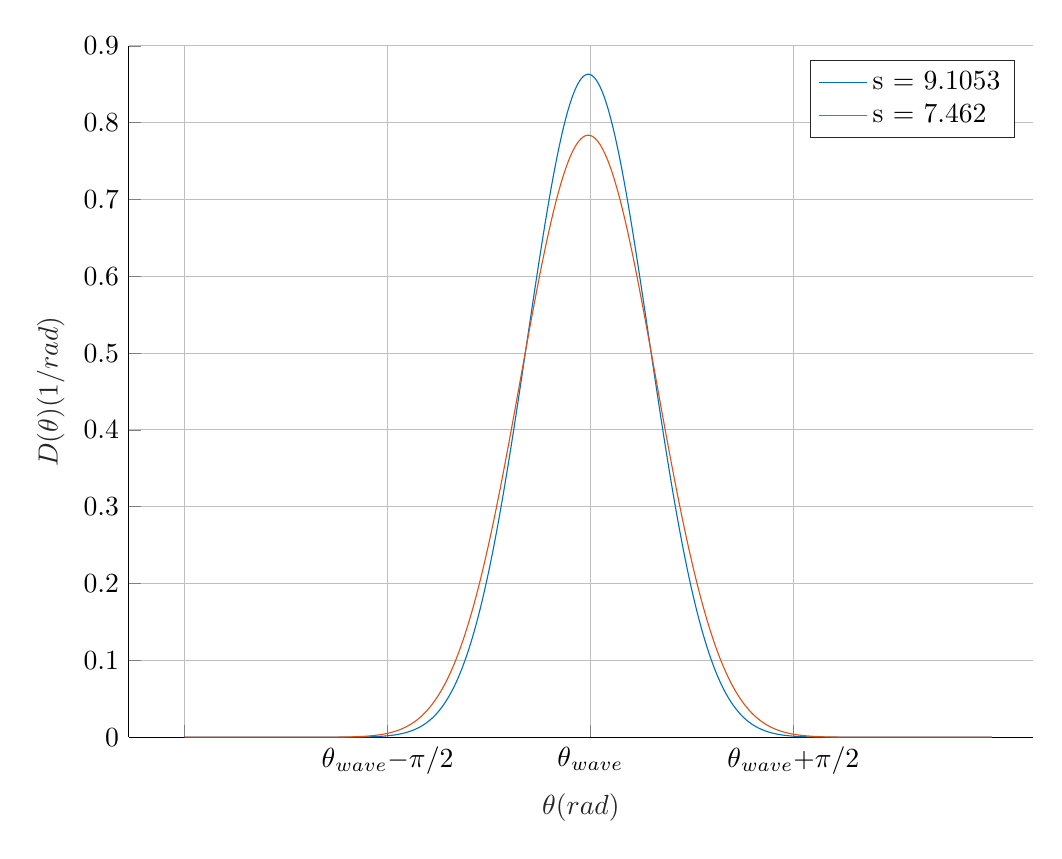
\begin{tikzpicture}

\begin{axis}[%
width=4.521in,
height=3.457in,
at={(0.758in,0.59in)},
scale only axis,
xmin=2,
xmax=9,
xtick={2.43247763855852,4.00327396535342,5.57407029214831,7.14486661894321},
xticklabels={{},{$\theta{}_{\text{wave}}\text{-}\pi\text{/2}$},{$\theta{}_{\text{wave}}$},{$\theta{}_{\text{wave}}\text{+}\pi\text{/2}$},{}},
xlabel style={font=\color{white!15!black}},
xlabel={$\theta\text{ (rad)}$},
ymin=0,
ymax=0.9,
ylabel style={font=\color{white!15!black}},
ylabel={$\text{D(}\theta\text{) (1/rad)}$},
axis background/.style={fill=white},
axis x line*=bottom,
axis y line*=left,
xmajorgrids,
ymajorgrids,
legend style={legend cell align=left, align=left, draw=white!15!black}
]
\addplot [color=mycolor1]
  table[row sep=crcr]{%
2.43247763855852	1.089904700123e-38\\
2.44470855832369	2.53928259637907e-34\\
2.45693947808885	1.59156982988422e-31\\
2.46917039785402	1.83553658139019e-29\\
2.48140131761919	7.89830854723131e-28\\
2.49363223738435	1.78097072613875e-26\\
2.50586315714952	2.54382636355025e-25\\
2.51809407691468	2.58652941526749e-24\\
2.53032499667985	2.02198059976341e-23\\
2.54255591644502	1.28197460650498e-22\\
2.55478683621018	6.85175917206531e-22\\
2.56701775597535	3.17735388940589e-21\\
2.57924867574052	1.30695963905769e-20\\
2.59147959550568	4.85180422302725e-20\\
2.60371051527085	1.64809000025001e-19\\
2.61594143503602	5.18026355870015e-19\\
2.62817235480118	1.52057306273369e-18\\
2.64040327456635	4.20017263999632e-18\\
2.65263419433151	1.09880994880626e-17\\
2.66486511409668	2.73742798874594e-17\\
2.67709603386185	6.52462467175746e-17\\
2.68932695362701	1.49386216186298e-16\\
2.70155787339218	3.29706380201836e-16\\
2.71378879315735	7.03613963297035e-16\\
2.72601971292251	1.45579369423918e-15\\
2.73825063268768	2.92722375793218e-15\\
2.75048155245284	5.73217896169244e-15\\
2.76271247221801	1.09524054371345e-14\\
2.77494339198318	2.04530626825874e-14\\
2.78717431174834	3.73874347540462e-14\\
2.79940523151351	6.69895012022819e-14\\
2.81163615127868	1.17798773683289e-13\\
2.82386707104384	2.03524962338879e-13\\
2.83609799080901	3.45846983681081e-13\\
2.84832891057418	5.78559138809039e-13\\
2.86055983033934	9.53636543450673e-13\\
2.87279075010451	1.55000403852659e-12\\
2.88502166986967	2.48607266817198e-12\\
2.89725258963484	3.93747358144406e-12\\
2.90948350940001	6.16189306796198e-12\\
2.92171442916517	9.53352117999145e-12\\
2.93394534893034	1.45904021804709e-11\\
2.94617626869551	2.20989561873611e-11\\
2.95840718846067	3.3141173155911e-11\\
2.97063810822584	4.92315159616555e-11\\
2.98286902799101	7.2472470913339e-11\\
2.99509994775617	1.05760023538176e-10\\
3.00733086752134	1.5305319791094e-10\\
3.0195617872865	2.19725274167878e-10\\
3.03179270705167	3.13018499338631e-10\\
3.04402362681684	4.42629153682584e-10\\
3.056254546582	6.21455866100742e-10\\
3.06848546634717	8.66551242044003e-10\\
3.08071638611234	1.20032534711118e-09\\
3.0929473058775	1.65205956887244e-09\\
3.10517822564267	2.25980106693913e-09\\
3.11740914540784	3.07272164500771e-09\\
3.129640065173	4.15404068650485e-09\\
3.14187098493817	5.58463005556968e-09\\
3.15410190470333	7.46743986538493e-09\\
3.1663328244685	9.93290806380005e-09\\
3.17856374423367	1.31455442080147e-08\\
3.19079466399883	1.73119089397122e-08\\
3.203025583764	2.26902458893821e-08\\
3.21525650352917	2.96020624076673e-08\\
3.22748742329433	3.84460000279712e-08\\
3.2397183430595	4.97143853023211e-08\\
3.25194926282466	6.401290702062e-08\\
3.26418018258983	8.20839272216927e-08\\
3.276411102355	1.04834001228712e-07\\
3.28864202212016	1.3336625657815e-07\\
3.30087294188533	1.6901836253135e-07\\
3.3131038616505	2.1340691121039e-07\\
3.32533478141566	2.68479128605085e-07\\
3.33756570118083	3.36572939038789e-07\\
3.349796620946	4.20486520395098e-07\\
3.36202754071116	5.23558609679019e-07\\
3.37425846047633	6.49760949435104e-07\\
3.38648938024149	8.03804405218241e-07\\
3.39872030000666	9.9126043267386e-07\\
3.41095121977183	1.21869972970344e-06\\
3.42318213953699	1.49385007443386e-06\\
3.43541305930216	1.82577552292645e-06\\
3.44764397906733	2.22507932128013e-06\\
3.45987489883249	2.70413307439155e-06\\
3.47210581859766	3.27733490738067e-06\\
3.48433673836283	3.96139955466092e-06\\
3.49656765812799	4.77568351475553e-06\\
3.50879857789316	5.74254861499264e-06\\
3.52102949765832	6.88776753772059e-06\\
3.53326041742349	8.24097506707168e-06\\
3.54549133718866	9.83616902075938e-06\\
3.55772225695382	1.17122650329346e-05\\
3.56995317671899	1.39137095495686e-05\\
3.58218409648416	1.6491155584785e-05\\
3.59441501624932	1.95022059624773e-05\\
3.60664593601449	2.30122289296466e-05\\
3.61887685577966	2.70952511732616e-05\\
3.63110777554482	3.18349333979574e-05\\
3.64333869530999	3.73256337242982e-05\\
3.65556961507515	4.36735642432158e-05\\
3.66780053484032	5.09980461080916e-05\\
3.68003145460549	5.94328685580818e-05\\
3.69226237437065	6.91277572410574e-05\\
3.70449329413582	8.02499571380708e-05\\
3.71672421390099	9.29859352798267e-05\\
3.72895513366615	0.000107543208285418\\
3.74118605343132	0.000124152299540766\\
3.75341697319648	0.000143068830565172\\
3.76564789296165	0.000164575750785491\\
3.77787881272682	0.000188985709545296\\
3.79010973249198	0.00021664357371777\\
3.80234065225715	0.000247929093762941\\
3.81457157202232	0.000283259720469646\\
3.82680249178748	0.00032309357394776\\
3.83903341155265	0.000367932565684954\\
3.85126433131782	0.000418325673652905\\
3.86349525108298	0.00047487236953937\\
3.87572617084815	0.000538226196194485\\
3.88795709061331	0.000609098492311888\\
3.90018801037848	0.000688262260218591\\
3.91241893014365	0.000776556171423222\\
3.92464984990881	0.000874888703272368\\
3.93688076967398	0.000984242398691782\\
3.94911168943915	0.00110567823954744\\
3.96134260920431	0.00124034012265378\\
3.97357352896948	0.00138945942588997\\
3.98580444873465	0.00155435965026386\\
3.99803536849981	0.00173646112209527\\
4.01026628826498	0.00193728573778349\\
4.02249720803014	0.00215846173188521\\
4.03472812779531	0.0024017284474701\\
4.04695904756048	0.00266894108595086\\
4.05918996732564	0.00296207541181323\\
4.07142088709081	0.00328323238591374\\
4.08365180685598	0.00363464269927725\\
4.09588272662114	0.00401867117763011\\
4.10811364638631	0.00443782102525945\\
4.12034456615148	0.0048947378752084\\
4.13257548591664	0.00539221361132012\\
4.14480640568181	0.00593318992623899\\
4.15703732544697	0.00652076157818838\\
4.16926824521214	0.00715817930818094\\
4.18149916497731	0.0078488523782974\\
4.19373008474247	0.00859635069081267\\
4.20596100450764	0.00940440644726175\\
4.21819192427281	0.0102769153060473\\
4.23042284403797	0.0112179369969052\\
4.24265376380314	0.0122316953504761\\
4.2548846835683	0.0133225777014083\\
4.26711560333347	0.0144951336238293\\
4.27934652309864	0.015754072958708\\
4.2915774428638	0.0171042630935826\\
4.30380836262897	0.0185507254563609\\
4.31603928239414	0.0200986311864302\\
4.3282702021593	0.0217532959481353\\
4.34050112192447	0.0235201738538139\\
4.35273204168964	0.0254048504660168\\
4.3649629614548	0.0274130348512846\\
4.37719388121997	0.0295505506609144\\
4.38942480098513	0.0318233262175123\\
4.4016557207503	0.034237383589802\\
4.41388664051547	0.0367988266421261\\
4.42611756028063	0.0395138280493386\\
4.4383484800458	0.042388615272323\\
4.45057939981097	0.0454294554941748\\
4.46281031957613	0.0486426395221425\\
4.4750412393413	0.0520344646657083\\
4.48727215910647	0.0556112166066892\\
4.49950307887163	0.059379150282928\\
4.5117339986368	0.0633444698129998\\
4.52396491840196	0.0675133074953516\\
4.53619583816713	0.071891701921398\\
4.5484267579323	0.0764855752482734\\
4.56065767769746	0.0813007096831768\\
4.57288859746263	0.0863427232374697\\
4.5851195172278	0.0916170448149217\\
4.59735043699296	0.0971288887046322\\
4.60958135675813	0.102883228555228\\
4.6218122765233	0.108884770912838\\
4.63404319628846	0.115137928411087\\
4.64627411605363	0.121646792706865\\
4.65850503581879	0.128415107260893\\
4.67073595558396	0.135446240067051\\
4.68296687534913	0.142743156439056\\
4.69519779511429	0.150308391967322\\
4.70742871487946	0.158144025762638\\
4.71965963464463	0.166251654106676\\
4.73189055440979	0.174632364632223\\
4.74412147417496	0.183286711158344\\
4.75635239394012	0.19221468930753\\
4.76858331370529	0.201415713033033\\
4.78081423347046	0.210888592185237\\
4.79304515323562	0.220631511245834\\
4.80527607300079	0.230642009357888\\
4.81750699276596	0.240916961778501\\
4.82973791253112	0.251452562878718\\
4.84196883229629	0.262244310812547\\
4.85419975206146	0.273286993973526\\
4.86643067182662	0.284574679353054\\
4.87866159159179	0.296100702909849\\
4.89089251135695	0.307857662054329\\
4.90312343112212	0.319837410345392\\
4.91535435088729	0.332031054490213\\
4.92758527065245	0.344428953730004\\
4.93981619041762	0.357020721686517\\
4.95204711018279	0.369795230735216\\
4.96427802994795	0.382740618961685\\
4.97650894971312	0.395844299747883\\
4.98873986947829	0.409092974024493\\
5.00097078924345	0.422472645214716\\
5.01320170900862	0.435968636883634\\
5.02543262877378	0.44956561309568\\
5.03766354853895	0.463247601470846\\
5.04989446830412	0.476998018918176\\
5.06212538806928	0.490799700012788\\
5.07435630783445	0.504634927970285\\
5.08658722759962	0.518485468159996\\
5.09881814736478	0.532332604086056\\
5.11104906712995	0.546157175753047\\
5.12327998689512	0.559939620320764\\
5.13551090666028	0.573660014940697\\
5.14774182642545	0.587298121655282\\
5.15997274619061	0.600833434229615\\
5.17220366595578	0.614245226774552\\
5.18443458572095	0.627512604009786\\
5.19666550548611	0.640614553005649\\
5.20889642525128	0.65352999623334\\
5.22112734501645	0.666237845744731\\
5.23335826478161	0.678717058295186\\
5.24558918454678	0.690946691215927\\
5.25782010431194	0.702905958836296\\
5.27005102407711	0.714574289251113\\
5.28228194384228	0.725931381223957\\
5.29451286360744	0.736957261013889\\
5.30674378337261	0.747632338910731\\
5.31897470313778	0.757937465262686\\
5.33120562290294	0.767853985779705\\
5.34343654266811	0.777363795896745\\
5.35566746243328	0.786449393982793\\
5.36789838219844	0.79509393318432\\
5.38012930196361	0.803281271695678\\
5.39236022172877	0.810996021253778\\
5.40459114149394	0.81822359366034\\
5.41682206125911	0.82495024514177\\
5.42905298102427	0.831163118364635\\
5.44128390078944	0.836850281933412\\
5.45351482055461	0.842000767206822\\
5.46574574031977	0.846604602279557\\
5.47797666008494	0.850652842987464\\
5.49020757985011	0.854137600806248\\
5.50243849961527	0.857052067526427\\
5.51466941938044	0.859390536600541\\
5.5269003391456	0.861148421072488\\
5.53913125891077	0.862322268013074\\
5.55136217867594	0.862909769400657\\
5.5635930984411	0.862909769400657\\
5.57582401820627	0.862322268013074\\
5.58805493797144	0.861148421072488\\
5.6002858577366	0.859390536600541\\
5.61251677750177	0.857052067526427\\
5.62474769726694	0.854137600806248\\
5.6369786170321	0.850652842987464\\
5.64920953679727	0.846604602279557\\
5.66144045656243	0.842000767206822\\
5.6736713763276	0.836850281933412\\
5.68590229609277	0.831163118364635\\
5.69813321585793	0.82495024514177\\
5.7103641356231	0.81822359366034\\
5.72259505538827	0.810996021253778\\
5.73482597515343	0.803281271695678\\
5.7470568949186	0.79509393318432\\
5.75928781468376	0.786449393982793\\
5.77151873444893	0.777363795896745\\
5.7837496542141	0.767853985779705\\
5.79598057397926	0.757937465262686\\
5.80821149374443	0.747632338910731\\
5.8204424135096	0.736957261013889\\
5.83267333327476	0.725931381223957\\
5.84490425303993	0.714574289251113\\
5.8571351728051	0.702905958836296\\
5.86936609257026	0.690946691215927\\
5.88159701233543	0.678717058295186\\
5.89382793210059	0.666237845744731\\
5.90605885186576	0.65352999623334\\
5.91828977163093	0.640614553005649\\
5.93052069139609	0.627512604009786\\
5.94275161116126	0.614245226774552\\
5.95498253092643	0.600833434229615\\
5.96721345069159	0.587298121655282\\
5.97944437045676	0.573660014940697\\
5.99167529022193	0.559939620320764\\
6.00390620998709	0.546157175753047\\
6.01613712975226	0.532332604086056\\
6.02836804951742	0.518485468159996\\
6.04059896928259	0.504634927970285\\
6.05282988904776	0.490799700012788\\
6.06506080881292	0.476998018918176\\
6.07729172857809	0.463247601470846\\
6.08952264834326	0.44956561309568\\
6.10175356810842	0.435968636883634\\
6.11398448787359	0.422472645214716\\
6.12621540763875	0.409092974024493\\
6.13844632740392	0.395844299747883\\
6.15067724716909	0.382740618961685\\
6.16290816693425	0.369795230735216\\
6.17513908669942	0.357020721686517\\
6.18737000646459	0.344428953730004\\
6.19960092622975	0.332031054490213\\
6.21183184599492	0.319837410345392\\
6.22406276576009	0.307857662054329\\
6.23629368552525	0.296100702909849\\
6.24852460529042	0.284574679353054\\
6.26075552505558	0.273286993973526\\
6.27298644482075	0.262244310812547\\
6.28521736458592	0.251452562878718\\
6.29744828435108	0.240916961778501\\
6.30967920411625	0.230642009357888\\
6.32191012388142	0.220631511245834\\
6.33414104364658	0.210888592185237\\
6.34637196341175	0.201415713033033\\
6.35860288317692	0.19221468930753\\
6.37083380294208	0.183286711158344\\
6.38306472270725	0.174632364632223\\
6.39529564247241	0.166251654106676\\
6.40752656223758	0.158144025762638\\
6.41975748200275	0.150308391967322\\
6.43198840176791	0.142743156439056\\
6.44421932153308	0.135446240067051\\
6.45645024129825	0.128415107260893\\
6.46868116106341	0.121646792706865\\
6.48091208082858	0.115137928411087\\
6.49314300059375	0.108884770912838\\
6.50537392035891	0.102883228555228\\
6.51760484012408	0.097128888704632\\
6.52983575988924	0.0916170448149217\\
6.54206667965441	0.0863427232374697\\
6.55429759941958	0.0813007096831768\\
6.56652851918474	0.0764855752482734\\
6.57875943894991	0.0718917019213976\\
6.59099035871508	0.0675133074953516\\
6.60322127848024	0.0633444698130001\\
6.61545219824541	0.059379150282928\\
6.62768311801057	0.0556112166066892\\
6.63991403777574	0.052034464665708\\
6.65214495754091	0.0486426395221425\\
6.66437587730607	0.045429455494175\\
6.67660679707124	0.042388615272323\\
6.68883771683641	0.0395138280493386\\
6.70106863660157	0.036798826642126\\
6.71329955636674	0.034237383589802\\
6.72553047613191	0.0318233262175125\\
6.73776139589707	0.0295505506609144\\
6.74999231566224	0.0274130348512846\\
6.76222323542741	0.0254048504660166\\
6.77445415519257	0.0235201738538139\\
6.78668507495774	0.0217532959481353\\
6.7989159947229	0.0200986311864302\\
6.81114691448807	0.0185507254563609\\
6.82337783425324	0.0171042630935825\\
6.8356087540184	0.015754072958708\\
6.84783967378357	0.0144951336238293\\
6.86007059354874	0.0133225777014083\\
6.8723015133139	0.0122316953504761\\
6.88453243307907	0.0112179369969052\\
6.89676335284423	0.0102769153060473\\
6.9089942726094	0.00940440644726175\\
6.92122519237457	0.00859635069081267\\
6.93345611213973	0.0078488523782974\\
6.9456870319049	0.00715817930818094\\
6.95791795167007	0.00652076157818838\\
6.97014887143523	0.00593318992623899\\
6.9823797912004	0.00539221361132012\\
6.99461071096557	0.0048947378752084\\
7.00684163073073	0.00443782102525945\\
7.0190725504959	0.00401867117763011\\
7.03130347026106	0.00363464269927725\\
7.04353439002623	0.00328323238591374\\
7.0557653097914	0.00296207541181323\\
7.06799622955656	0.00266894108595086\\
7.08022714932173	0.0024017284474701\\
7.0924580690869	0.00215846173188521\\
7.10468898885206	0.00193728573778349\\
7.11691990861723	0.00173646112209527\\
7.12915082838239	0.00155435965026386\\
7.14138174814756	0.00138945942588997\\
7.15361266791273	0.00124034012265378\\
7.16584358767789	0.00110567823954744\\
7.17807450744306	0.000984242398691782\\
7.19030542720823	0.000874888703272368\\
7.20253634697339	0.000776556171423222\\
7.21476726673856	0.000688262260218591\\
7.22699818650373	0.000609098492311891\\
7.23922910626889	0.000538226196194485\\
7.25146002603406	0.00047487236953937\\
7.26369094579923	0.000418325673652904\\
7.27592186556439	0.000367932565684954\\
7.28815278532956	0.000323093573947761\\
7.30038370509472	0.000283259720469646\\
7.31261462485989	0.000247929093762941\\
7.32484554462506	0.000216643573717768\\
7.33707646439022	0.000188985709545296\\
7.34930738415539	0.000164575750785491\\
7.36153830392056	0.000143068830565172\\
7.37376922368572	0.000124152299540766\\
7.38600014345089	0.000107543208285418\\
7.39823106321605	9.29859352798267e-05\\
7.41046198298122	8.02499571380708e-05\\
7.42269290274639	6.91277572410574e-05\\
7.43492382251155	5.94328685580818e-05\\
7.44715474227672	5.09980461080919e-05\\
7.45938566204189	4.36735642432158e-05\\
7.47161658180705	3.73256337242982e-05\\
7.48384750157222	3.18349333979574e-05\\
7.49607842133739	2.70952511732616e-05\\
7.50830934110255	2.30122289296467e-05\\
7.52054026086772	1.95022059624773e-05\\
7.53277118063288	1.6491155584785e-05\\
7.54500210039805	1.39137095495685e-05\\
7.55723302016322	1.17122650329346e-05\\
7.56946393992838	9.83616902075941e-06\\
7.58169485969355	8.24097506707168e-06\\
7.59392577945872	6.88776753772059e-06\\
7.60615669922388	5.7425486149926e-06\\
7.61838761898905	4.77568351475553e-06\\
7.63061853875421	3.96139955466092e-06\\
7.64284945851938	3.27733490738067e-06\\
7.65508037828455	2.70413307439155e-06\\
7.66731129804971	2.22507932128011e-06\\
7.67954221781488	1.82577552292645e-06\\
7.69177313758005	1.49385007443386e-06\\
7.70400405734521	1.21869972970344e-06\\
7.71623497711038	9.9126043267386e-07\\
7.72846589687555	8.03804405218248e-07\\
7.74069681664071	6.49760949435104e-07\\
7.75292773640588	5.23558609679019e-07\\
7.76515865617105	4.20486520395094e-07\\
7.77738957593621	3.36572939038789e-07\\
7.78962049570138	2.68479128605087e-07\\
7.80185141546654	2.1340691121039e-07\\
7.81408233523171	1.6901836253135e-07\\
7.82631325499688	1.33366256578149e-07\\
7.83854417476204	1.04834001228712e-07\\
7.85077509452721	8.20839272216935e-08\\
7.86300601429238	6.401290702062e-08\\
7.87523693405754	4.97143853023211e-08\\
7.88746785382271	3.84460000279708e-08\\
7.89969877358787	2.96020624076673e-08\\
7.91192969335304	2.26902458893823e-08\\
7.92416061311821	1.73119089397122e-08\\
7.93639153288337	1.31455442080147e-08\\
7.94862245264854	9.93290806379994e-09\\
7.96085337241371	7.46743986538493e-09\\
7.97308429217887	5.58463005556968e-09\\
7.98531521194404	4.15404068650485e-09\\
7.99754613170921	3.07272164500771e-09\\
8.00977705147437	2.25980106693916e-09\\
8.02200797123954	1.65205956887241e-09\\
8.0342388910047	1.20032534711116e-09\\
8.04646981076987	8.66551242043995e-10\\
8.05870073053504	6.21455866100742e-10\\
8.0709316503002	4.42629153682589e-10\\
8.08316257006537	3.13018499338639e-10\\
8.09539348983053	2.19725274167884e-10\\
8.1076244095957	1.53053197910938e-10\\
8.11985532936087	1.05760023538176e-10\\
8.13208624912603	7.24724709133401e-11\\
8.1443171688912	4.92315159616541e-11\\
8.15654808865637	3.31411731559101e-11\\
8.16877900842153	2.20989561873608e-11\\
8.1810099281867	1.45904021804709e-11\\
8.19324084795187	9.53352117999161e-12\\
8.20547176771703	6.16189306796218e-12\\
8.2177026874822	3.93747358144419e-12\\
8.22993360724737	2.48607266817194e-12\\
8.24216452701253	1.55000403852659e-12\\
8.2543954467777	9.53636543450691e-13\\
8.26662636654287	5.78559138809006e-13\\
8.27885728630803	3.45846983681068e-13\\
8.2910882060732	2.03524962338875e-13\\
8.30331912583836	1.17798773683289e-13\\
8.31555004560353	6.69895012022819e-14\\
8.3277809653687	3.7387434754047e-14\\
8.34001188513386	2.04530626825883e-14\\
8.35224280489903	1.09524054371353e-14\\
8.3644737246642	5.73217896169244e-15\\
8.37670464442936	2.92722375793218e-15\\
8.38893556419453	1.45579369423906e-15\\
8.4011664839597	7.03613963296996e-16\\
8.41339740372486	3.29706380201827e-16\\
8.42562832349003	1.49386216186298e-16\\
8.43785924325519	6.52462467175746e-17\\
8.45009016302036	2.73742798874603e-17\\
8.46232108278553	1.09880994880633e-17\\
8.47455200255069	4.20017263999677e-18\\
8.48678292231586	1.52057306273369e-18\\
8.49901384208103	5.18026355870015e-19\\
8.51124476184619	1.6480900002498e-19\\
8.52347568161136	4.8518042230268e-20\\
8.53570660137652	1.30695963905762e-20\\
8.54793752114169	3.17735388940572e-21\\
8.56016844090686	6.85175917206531e-22\\
8.57239936067202	1.28197460650506e-22\\
8.58463028043719	2.02198059976369e-23\\
8.59686120020235	2.58652941526811e-24\\
8.60909211996752	2.54382636355002e-25\\
8.62132303973269	1.78097072613875e-26\\
8.63355395949785	7.89830854723228e-28\\
8.64578487926302	1.83553658138963e-29\\
8.65801579902819	1.59156982988359e-31\\
8.67024671879335	2.53928259637836e-34\\
8.68247763855852	1.089904700123e-38\\
};
\addlegendentry{s = 9.1053}

\addplot [color=mycolor2]
  table[row sep=crcr]{%
2.43247763855852	6.84426576490762e-32\\
2.44470855832369	2.59684421254285e-28\\
2.45693947808885	5.09031053663978e-26\\
2.46917039785402	2.4920015713877e-24\\
2.48140131761919	5.43826588035286e-23\\
2.49363223738435	6.98835427276338e-22\\
2.50586315714952	6.17710002045318e-21\\
2.51809407691468	4.13268438829053e-20\\
2.53032499667985	2.22902345680389e-19\\
2.54255591644502	1.01264128317249e-18\\
2.55478683621018	3.99949011287495e-18\\
2.56701775597535	1.40612053604555e-17\\
2.57924867574052	4.48095383455307e-17\\
2.59147959550568	1.31281689597087e-16\\
2.60371051527085	3.57630246628581e-16\\
2.61594143503602	9.14199349977807e-16\\
2.62817235480118	2.2095053492284e-15\\
2.64040327456635	5.08062836848848e-15\\
2.65263419433151	1.11736601318794e-14\\
2.66486511409668	2.3608623304748e-14\\
2.67709603386185	4.8106644131395e-14\\
2.68932695362701	9.48489157915017e-14\\
2.70155787339218	1.8146713881386e-13\\
2.71378879315735	3.37746310525779e-13\\
2.72601971292251	6.12868709411088e-13\\
2.73825063268768	1.08636204918599e-12\\
2.75048155245284	1.88435858499321e-12\\
2.76271247221801	3.20335369153897e-12\\
2.77494339198318	5.34440567241069e-12\\
2.78717431174834	8.76168280267586e-12\\
2.79940523151351	1.41304848981191e-11\\
2.81163615127868	2.24413982423792e-11\\
2.82386707104384	3.51291454333504e-11\\
2.83609799080901	5.42470348910369e-11\\
2.84832891057418	8.27007764959723e-11\\
2.86055983033934	1.24558897500168e-10\\
2.87279075010451	1.85461163572134e-10\\
2.88502166986967	2.73151390714857e-10\\
2.89725258963484	3.98166942159013e-10\\
2.90948350940001	5.74724167815331e-10\\
2.92171442916517	8.21847200359553e-10\\
2.93394534893034	1.16479701946731e-09\\
2.94617626869551	1.63686869175496e-09\\
2.95840718846067	2.28163735540103e-09\\
2.97063810822584	3.15574802041381e-09\\
2.98286902799101	4.33236078072311e-09\\
2.99509994775617	5.90538177164993e-09\\
3.00733086752134	7.99463134969229e-09\\
3.0195617872865	1.07521247180757e-08\\
3.03179270705167	1.43696667696885e-08\\
3.04402362681684	1.90879924666974e-08\\
3.056254546582	2.52077168181265e-08\\
3.06848546634717	3.31023946421898e-08\\
3.08071638611234	4.32340299899673e-08\\
3.0929473058775	5.61714185304473e-08\\
3.10517822564267	7.26117535086908e-08\\
3.11740914540784	9.34059772254328e-08\\
3.129640065173	1.1958841546273e-07\\
3.14187098493817	1.52411291985674e-07\\
3.15410190470333	1.93384784244843e-07\\
3.1663328244685	2.44323349715085e-07\\
3.17856374423367	3.07399124922778e-07\\
3.19079466399883	3.85203276084701e-07\\
3.203025583764	4.8081626130983e-07\\
3.21525650352917	5.97888049354828e-07\\
3.22748742329433	7.4072942877584e-07\\
3.2397183430595	9.1441563372722e-07\\
3.25194926282466	1.12490360830653e-06\\
3.26418018258983	1.37916432985505e-06\\
3.276411102355	1.68533171254832e-06\\
3.28864202212016	2.05286971543832e-06\\
3.30087294188533	2.49275938325127e-06\\
3.3131038616505	3.01770765304587e-06\\
3.32533478141566	3.64237986456376e-06\\
3.33756570118083	4.3836580159508e-06\\
3.349796620946	5.26092690861487e-06\\
3.36202754071116	6.29639042435793e-06\\
3.37425846047633	7.51542027355113e-06\\
3.38648938024149	8.94693964391559e-06\\
3.39872030000666	1.06238442642619e-05\\
3.41095121977183	1.25834634751042e-05\\
3.42318213953699	1.48680639671076e-05\\
3.43541305930216	1.75253989075134e-05\\
3.44764397906733	2.06093052226282e-05\\
3.45987489883249	2.41803518397176e-05\\
3.47210581859766	2.83065417127732e-05\\
3.48433673836283	3.30640704621109e-05\\
3.49656765812799	3.853814444612e-05\\
3.50879857789316	4.48238610532197e-05\\
3.52102949765832	5.20271539516553e-05\\
3.53326041742349	6.02658059627537e-05\\
3.54549133718866	6.96705321281542e-05\\
3.55772225695382	8.03861354219498e-05\\
3.56995317671899	9.25727374132859e-05\\
3.58218409648416	0.000106407086012439\\
3.59441501624932	0.000122083942232593\\
3.60664593601449	0.000139817547669329\\
3.61887685577966	0.000159843174139253\\
3.63110777554482	0.0001824187566274\\
3.64333869530999	0.000207826610369319\\
3.65556961507515	0.000236375232537543\\
3.66780053484032	0.000268401188613145\\
3.68003145460549	0.000304271083100975\\
3.69226237437065	0.000344383613792176\\
3.70449329413582	0.000389171708289732\\
3.71672421390099	0.000439104740992663\\
3.72895513366615	0.000494690828182821\\
3.74118605343132	0.000556479198275778\\
3.75341697319648	0.000625062633685549\\
3.76564789296165	0.000701079980113047\\
3.77787881272682	0.000785218718402108\\
3.79010973249198	0.000878217593416764\\
3.80234065225715	0.000980869293681067\\
3.81457157202232	0.00109402317479147\\
3.82680249178748	0.0012185880188636\\
3.83903341155265	0.00135553482151384\\
3.85126433131782	0.00150589959710511\\
3.86349525108298	0.00167078619220823\\
3.87572617084815	0.00185136909645068\\
3.88795709061331	0.00204889623914627\\
3.90018801037848	0.00226469175932743\\
3.91241893014365	0.00250015873604099\\
3.92464984990881	0.00275678186502289\\
3.93688076967398	0.00303613006714268\\
3.94911168943915	0.00333985901331071\\
3.96134260920431	0.00366971354987211\\
3.97357352896948	0.00402753000788263\\
3.98580444873465	0.00441523837907145\\
3.99803536849981	0.00483486434075526\\
4.01026628826498	0.00528853111148142\\
4.02249720803014	0.00577846111874734\\
4.03472812779531	0.00630697745978007\\
4.04695904756048	0.00687650513606537\\
4.05918996732564	0.00748957204209489\\
4.07142088709081	0.00814880968866243\\
4.08365180685598	0.00885695364098502\\
4.09588272662114	0.00961684365196081\\
4.10811364638631	0.0104314234710082\\
4.12034456615148	0.0113037403091561\\
4.13257548591664	0.012236943941392\\
4.14480640568181	0.0132342854277081\\
4.15703732544697	0.0142991154348344\\
4.16926824521214	0.0154348821413079\\
4.18149916497731	0.0166451287092941\\
4.19373008474247	0.0179334903074723\\
4.20596100450764	0.0193036906702902\\
4.21819192427281	0.0207595381800227\\
4.23042284403797	0.0223049214593022\\
4.24265376380314	0.0239438044631396\\
4.2548846835683	0.0256802210609266\\
4.26711560333347	0.027518269100485\\
4.27934652309864	0.029462103947919\\
4.2915774428638	0.0315159314988248\\
4.30380836262897	0.0336840006582995\\
4.31603928239414	0.0359705952891977\\
4.3282702021593	0.0383800256301567\\
4.34050112192447	0.0409166191870887\\
4.35273204168964	0.0435847111040871\\
4.3649629614548	0.0463886340220073\\
4.37719388121997	0.0493327074353715\\
4.38942480098513	0.0524212265606736\\
4.4016557207503	0.0556584507316479\\
4.41388664051547	0.0590485913395698\\
4.42611756028063	0.0625957993392011\\
4.4383484800458	0.0663041523435348\\
4.45057939981097	0.0701776413330474\\
4.46281031957613	0.0742201570077034\\
4.4750412393413	0.0784354758124742\\
4.48727215910647	0.0828272456696125\\
4.49950307887163	0.0873989714533506\\
4.5117339986368	0.0921540002450668\\
4.52396491840196	0.0970955064092514\\
4.53619583816713	0.102226476532818\\
4.5484267579323	0.107549694272403\\
4.56065767769746	0.113067725156308\\
4.57288859746263	0.118782901389565\\
4.5851195172278	0.124697306712388\\
4.59735043699296	0.130812761363796\\
4.60958135675813	0.137130807203639\\
4.6218122765233	0.143652693047481\\
4.63404319628846	0.150379360269847\\
4.64627411605363	0.157311428732199\\
4.65850503581879	0.164449183092655\\
4.67073595558396	0.171792559554911\\
4.68296687534913	0.179341133113998\\
4.69519779511429	0.18709410535657\\
4.70742871487946	0.195050292873076\\
4.71965963464463	0.203208116338726\\
4.73189055440979	0.21156559031944\\
4.74412147417496	0.220120313857914\\
4.75635239394012	0.228869461893779\\
4.76858331370529	0.237809777570267\\
4.78081423347046	0.246937565478109\\
4.79304515323562	0.256248685885377\\
4.80527607300079	0.265738549999737\\
4.81750699276596	0.275402116307111\\
4.82973791253112	0.285233888028025\\
4.84196883229629	0.295227911729956\\
4.85419975206146	0.305377777130831\\
4.86643067182662	0.315676618125422\\
4.87866159159179	0.326117115062814\\
4.89089251135695	0.336691498299288\\
4.90312343112212	0.347391553047031\\
4.91535435088729	0.358208625534935\\
4.92758527065245	0.369133630493423\\
4.93981619041762	0.380157059970869\\
4.95204711018279	0.391268993484553\\
4.96427802994795	0.402459109504513\\
4.97650894971312	0.413716698263835\\
4.98873986947829	0.42503067588419\\
5.00097078924345	0.436389599800503\\
5.01320170900862	0.447781685463791\\
5.02543262877378	0.459194824296311\\
5.03766354853895	0.470616602868271\\
5.04989446830412	0.482034323260515\\
5.06212538806928	0.493435024572821\\
5.07435630783445	0.504805505532714\\
5.08658722759962	0.516132348155113\\
5.09881814736478	0.527401942398615\\
5.11104906712995	0.53860051175989\\
5.12327998689512	0.549714139743466\\
5.13551090666028	0.560728797140157\\
5.14774182642545	0.571630370043614\\
5.15997274619061	0.582404688530857\\
5.17220366595578	0.593037555929328\\
5.18443458572095	0.603514778589902\\
5.19666550548611	0.613822196082433\\
5.20889642525128	0.623945711727944\\
5.22112734501645	0.633871323379284\\
5.23335826478161	0.643585154360152\\
5.24558918454678	0.653073484470813\\
5.25782010431194	0.662322780967561\\
5.27005102407711	0.671319729422027\\
5.28228194384228	0.680051264365929\\
5.29451286360744	0.688504599626558\\
5.30674378337261	0.696667258258532\\
5.31897470313778	0.704527101977769\\
5.33120562290294	0.712072360004579\\
5.34343654266811	0.719291657223938\\
5.35566746243328	0.726174041572672\\
5.36789838219844	0.732709010565163\\
5.38012930196361	0.738886536871543\\
5.39236022172877	0.744697092864937\\
5.40459114149394	0.750131674057348\\
5.41682206125911	0.755181821347026\\
5.42905298102427	0.759839642003808\\
5.44128390078944	0.764097829322829\\
5.45351482055461	0.767949680881161\\
5.46574574031977	0.771389115336451\\
5.47797666008494	0.774410687711302\\
5.49020757985011	0.777009603112092\\
5.50243849961527	0.779181728836089\\
5.51466941938044	0.780923604826031\\
5.5269003391456	0.782232452436912\\
5.53913125891077	0.78310618148529\\
5.55136217867594	0.78354339555729\\
5.5635930984411	0.78354339555729\\
5.57582401820627	0.78310618148529\\
5.58805493797144	0.782232452436912\\
5.6002858577366	0.780923604826031\\
5.61251677750177	0.779181728836089\\
5.62474769726694	0.777009603112092\\
5.6369786170321	0.774410687711302\\
5.64920953679727	0.771389115336451\\
5.66144045656243	0.767949680881161\\
5.6736713763276	0.764097829322829\\
5.68590229609277	0.759839642003808\\
5.69813321585793	0.755181821347026\\
5.7103641356231	0.750131674057348\\
5.72259505538827	0.744697092864937\\
5.73482597515343	0.738886536871543\\
5.7470568949186	0.732709010565163\\
5.75928781468376	0.726174041572672\\
5.77151873444893	0.719291657223938\\
5.7837496542141	0.712072360004579\\
5.79598057397926	0.704527101977769\\
5.80821149374443	0.696667258258532\\
5.8204424135096	0.688504599626558\\
5.83267333327476	0.680051264365929\\
5.84490425303993	0.671319729422027\\
5.8571351728051	0.662322780967561\\
5.86936609257026	0.653073484470813\\
5.88159701233543	0.643585154360152\\
5.89382793210059	0.633871323379284\\
5.90605885186576	0.623945711727944\\
5.91828977163093	0.613822196082433\\
5.93052069139609	0.603514778589902\\
5.94275161116126	0.593037555929328\\
5.95498253092643	0.582404688530857\\
5.96721345069159	0.571630370043614\\
5.97944437045676	0.560728797140157\\
5.99167529022193	0.549714139743466\\
6.00390620998709	0.53860051175989\\
6.01613712975226	0.527401942398615\\
6.02836804951742	0.516132348155113\\
6.04059896928259	0.504805505532714\\
6.05282988904776	0.493435024572821\\
6.06506080881292	0.482034323260515\\
6.07729172857809	0.470616602868271\\
6.08952264834326	0.459194824296311\\
6.10175356810842	0.447781685463791\\
6.11398448787359	0.436389599800503\\
6.12621540763875	0.42503067588419\\
6.13844632740392	0.413716698263835\\
6.15067724716909	0.402459109504513\\
6.16290816693425	0.391268993484553\\
6.17513908669942	0.380157059970869\\
6.18737000646459	0.369133630493423\\
6.19960092622975	0.358208625534935\\
6.21183184599492	0.347391553047031\\
6.22406276576009	0.336691498299288\\
6.23629368552525	0.326117115062814\\
6.24852460529042	0.315676618125422\\
6.26075552505558	0.305377777130831\\
6.27298644482075	0.295227911729956\\
6.28521736458592	0.285233888028025\\
6.29744828435108	0.275402116307111\\
6.30967920411625	0.265738549999737\\
6.32191012388142	0.256248685885377\\
6.33414104364658	0.246937565478109\\
6.34637196341175	0.237809777570267\\
6.35860288317692	0.228869461893779\\
6.37083380294208	0.220120313857914\\
6.38306472270725	0.21156559031944\\
6.39529564247241	0.203208116338726\\
6.40752656223758	0.195050292873076\\
6.41975748200275	0.18709410535657\\
6.43198840176791	0.179341133113998\\
6.44421932153308	0.171792559554911\\
6.45645024129825	0.164449183092655\\
6.46868116106341	0.157311428732199\\
6.48091208082858	0.150379360269847\\
6.49314300059375	0.143652693047481\\
6.50537392035891	0.137130807203639\\
6.51760484012408	0.130812761363795\\
6.52983575988924	0.124697306712388\\
6.54206667965441	0.118782901389565\\
6.55429759941958	0.113067725156308\\
6.56652851918474	0.107549694272403\\
6.57875943894991	0.102226476532817\\
6.59099035871508	0.0970955064092514\\
6.60322127848024	0.0921540002450671\\
6.61545219824541	0.0873989714533506\\
6.62768311801057	0.0828272456696125\\
6.63991403777574	0.0784354758124739\\
6.65214495754091	0.0742201570077034\\
6.66437587730607	0.0701776413330477\\
6.67660679707124	0.0663041523435348\\
6.68883771683641	0.0625957993392011\\
6.70106863660157	0.0590485913395696\\
6.71329955636674	0.0556584507316479\\
6.72553047613191	0.0524212265606738\\
6.73776139589707	0.0493327074353715\\
6.74999231566224	0.0463886340220073\\
6.76222323542741	0.0435847111040868\\
6.77445415519257	0.0409166191870887\\
6.78668507495774	0.0383800256301567\\
6.7989159947229	0.0359705952891977\\
6.81114691448807	0.0336840006582995\\
6.82337783425324	0.0315159314988246\\
6.8356087540184	0.029462103947919\\
6.84783967378357	0.027518269100485\\
6.86007059354874	0.0256802210609266\\
6.8723015133139	0.0239438044631396\\
6.88453243307907	0.0223049214593022\\
6.89676335284423	0.0207595381800227\\
6.9089942726094	0.0193036906702902\\
6.92122519237457	0.0179334903074723\\
6.93345611213973	0.0166451287092941\\
6.9456870319049	0.0154348821413079\\
6.95791795167007	0.0142991154348344\\
6.97014887143523	0.0132342854277081\\
6.9823797912004	0.012236943941392\\
6.99461071096557	0.0113037403091561\\
7.00684163073073	0.0104314234710082\\
7.0190725504959	0.00961684365196081\\
7.03130347026106	0.00885695364098502\\
7.04353439002623	0.00814880968866243\\
7.0557653097914	0.00748957204209489\\
7.06799622955656	0.00687650513606537\\
7.08022714932173	0.00630697745978007\\
7.0924580690869	0.00577846111874734\\
7.10468898885206	0.00528853111148142\\
7.11691990861723	0.00483486434075526\\
7.12915082838239	0.00441523837907145\\
7.14138174814756	0.00402753000788263\\
7.15361266791273	0.00366971354987211\\
7.16584358767789	0.00333985901331072\\
7.17807450744306	0.00303613006714268\\
7.19030542720823	0.00275678186502289\\
7.20253634697339	0.00250015873604099\\
7.21476726673856	0.00226469175932743\\
7.22699818650373	0.00204889623914628\\
7.23922910626889	0.00185136909645068\\
7.25146002603406	0.00167078619220823\\
7.26369094579923	0.0015058995971051\\
7.27592186556439	0.00135553482151384\\
7.28815278532956	0.0012185880188636\\
7.30038370509472	0.00109402317479147\\
7.31261462485989	0.000980869293681067\\
7.32484554462506	0.00087821759341676\\
7.33707646439022	0.000785218718402108\\
7.34930738415539	0.000701079980113047\\
7.36153830392056	0.000625062633685549\\
7.37376922368572	0.000556479198275778\\
7.38600014345089	0.000494690828182819\\
7.39823106321605	0.000439104740992663\\
7.41046198298122	0.000389171708289732\\
7.42269290274639	0.000344383613792176\\
7.43492382251155	0.000304271083100975\\
7.44715474227672	0.000268401188613147\\
7.45938566204189	0.000236375232537543\\
7.47161658180705	0.000207826610369319\\
7.48384750157222	0.0001824187566274\\
7.49607842133739	0.000159843174139253\\
7.50830934110255	0.000139817547669329\\
7.52054026086772	0.000122083942232593\\
7.53277118063288	0.000106407086012439\\
7.54500210039805	9.25727374132854e-05\\
7.55723302016322	8.03861354219498e-05\\
7.56946393992838	6.96705321281544e-05\\
7.58169485969355	6.02658059627537e-05\\
7.59392577945872	5.20271539516553e-05\\
7.60615669922388	4.48238610532194e-05\\
7.61838761898905	3.853814444612e-05\\
7.63061853875421	3.30640704621109e-05\\
7.64284945851938	2.83065417127732e-05\\
7.65508037828455	2.41803518397176e-05\\
7.66731129804971	2.06093052226281e-05\\
7.67954221781488	1.75253989075134e-05\\
7.69177313758005	1.48680639671076e-05\\
7.70400405734521	1.25834634751042e-05\\
7.71623497711038	1.06238442642619e-05\\
7.72846589687555	8.94693964391566e-06\\
7.74069681664071	7.51542027355113e-06\\
7.75292773640588	6.29639042435793e-06\\
7.76515865617105	5.26092690861483e-06\\
7.77738957593621	4.3836580159508e-06\\
7.78962049570138	3.64237986456379e-06\\
7.80185141546654	3.01770765304587e-06\\
7.81408233523171	2.49275938325127e-06\\
7.82631325499688	2.05286971543831e-06\\
7.83854417476204	1.68533171254832e-06\\
7.85077509452721	1.37916432985506e-06\\
7.86300601429238	1.12490360830653e-06\\
7.87523693405754	9.1441563372722e-07\\
7.88746785382271	7.40729428775834e-07\\
7.89969877358787	5.97888049354828e-07\\
7.91192969335304	4.80816261309833e-07\\
7.92416061311821	3.85203276084701e-07\\
7.93639153288337	3.07399124922778e-07\\
7.94862245264854	2.44323349715083e-07\\
7.96085337241371	1.93384784244843e-07\\
7.97308429217887	1.52411291985674e-07\\
7.98531521194404	1.1958841546273e-07\\
7.99754613170921	9.34059772254328e-08\\
8.00977705147437	7.26117535086915e-08\\
8.02200797123954	5.61714185304463e-08\\
8.0342388910047	4.32340299899665e-08\\
8.04646981076987	3.31023946421896e-08\\
8.05870073053504	2.52077168181265e-08\\
8.0709316503002	1.90879924666976e-08\\
8.08316257006537	1.43696667696888e-08\\
8.09539348983053	1.07521247180759e-08\\
8.1076244095957	7.9946313496922e-09\\
8.11985532936087	5.90538177164993e-09\\
8.13208624912603	4.33236078072316e-09\\
8.1443171688912	3.15574802041373e-09\\
8.15654808865637	2.28163735540098e-09\\
8.16877900842153	1.63686869175494e-09\\
8.1810099281867	1.16479701946731e-09\\
8.19324084795187	8.21847200359564e-10\\
8.20547176771703	5.74724167815347e-10\\
8.2177026874822	3.98166942159023e-10\\
8.22993360724737	2.73151390714853e-10\\
8.24216452701253	1.85461163572134e-10\\
8.2543954467777	1.2455889750017e-10\\
8.26662636654287	8.27007764959685e-11\\
8.27885728630803	5.42470348910351e-11\\
8.2910882060732	3.51291454333498e-11\\
8.30331912583836	2.24413982423792e-11\\
8.31555004560353	1.41304848981191e-11\\
8.3277809653687	8.76168280267602e-12\\
8.34001188513386	5.34440567241089e-12\\
8.35224280489903	3.20335369153915e-12\\
8.3644737246642	1.88435858499321e-12\\
8.37670464442936	1.08636204918599e-12\\
8.38893556419453	6.12868709411049e-13\\
8.4011664839597	3.37746310525764e-13\\
8.41339740372486	1.81467138813855e-13\\
8.42562832349003	9.48489157915017e-14\\
8.43785924325519	4.8106644131395e-14\\
8.45009016302036	2.36086233047487e-14\\
8.46232108278553	1.11736601318801e-14\\
8.47455200255069	5.08062836848893e-15\\
8.48678292231586	2.2095053492284e-15\\
8.49901384208103	9.14199349977807e-16\\
8.51124476184619	3.57630246628543e-16\\
8.52347568161136	1.31281689597077e-16\\
8.53570660137652	4.48095383455288e-17\\
8.54793752114169	1.40612053604549e-17\\
8.56016844090686	3.99949011287495e-18\\
8.57239936067202	1.01264128317255e-18\\
8.58463028043719	2.22902345680415e-19\\
8.59686120020235	4.13268438829133e-20\\
8.60909211996752	6.17710002045272e-21\\
8.62132303973269	6.98835427276338e-22\\
8.63355395949785	5.43826588035341e-23\\
8.64578487926302	2.49200157138708e-24\\
8.65801579902819	5.09031053663813e-26\\
8.67024671879335	2.59684421254226e-28\\
8.68247763855852	6.84426576490762e-32\\
};
\addlegendentry{s = 7.462}

\end{axis}
\end{tikzpicture}%}
    \caption{Directional distribution function, $D(\theta)$, defined using the $\cos^2(\theta)$ model detailed in Section \ref{subsec:theory.waves.modelling}.}
    \label{fig:systemDesign.direcDistributionFunction}
\end{figure}

% Generate 2D spectrum from 1D eq
In accordance with Equation xx, the two-dimensional directional wave spectrum can be obtained by multiplying the one-dimensional wave spectrum, $E(\omega)$, with the directional distribution function, $D(\theta)$. This was achieved using the \href{https://github.com/JNSRYA006/sar-parameter-extraction-pipeline/blob/main/functions/waveSpectra/generate2DWaveSpectrum.m}{\lstinline{generate2DWaveSpectrum}} block, which took in the one-dimensional wave spectrum, and the directional distribution function and simply performed an element-wise multiplication using \textsc{Matlab}'s built-in 'dot' multiplication. This resulted in the two-dimensional wave spectrum shown in Figure \ref{fig:systemDesign.2DSampleWaveSpectrum}
% INCREASE SURF FONT SIZE
\begin{figure} [H]
    \centering
    \subcaptionbox{Contour plot of the two-dimensional wave spectrum, E($\omega,\theta$). \label{fig:systemDesign.2DSampleWaveSpectrumContour}}[0.48\linewidth]{
        \resizebox{\linewidth}{!}{% This file was created by matlab2tikz.
%
%The latest updates can be retrieved from
%  http://www.mathworks.com/matlabcentral/fileexchange/22022-matlab2tikz-matlab2tikz
%where you can also make suggestions and rate matlab2tikz.
%
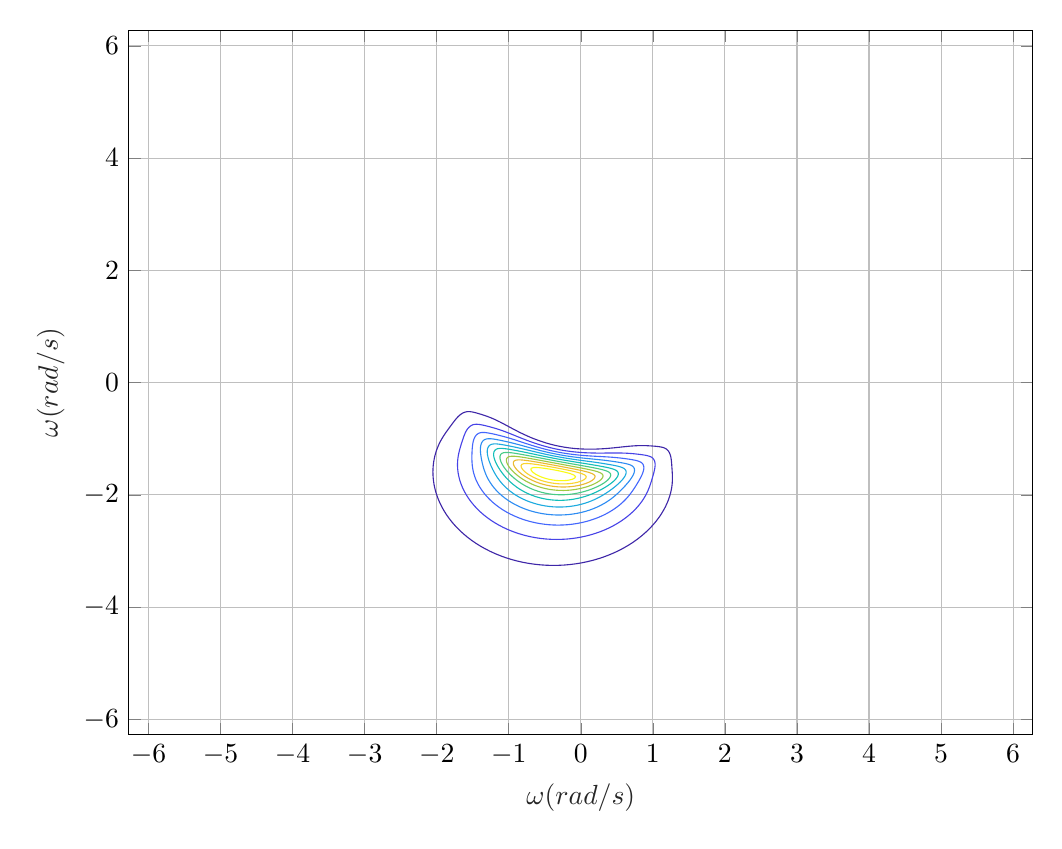
\begin{tikzpicture}

\begin{axis}[%
width=4.521in,
height=3.522in,
at={(0.758in,0.525in)},
scale only axis,
colormap={mymap}{[1pt] rgb(0pt)=(0.2422,0.1504,0.6603); rgb(1pt)=(0.2444,0.1534,0.6728); rgb(2pt)=(0.2464,0.1569,0.6847); rgb(3pt)=(0.2484,0.1607,0.6961); rgb(4pt)=(0.2503,0.1648,0.7071); rgb(5pt)=(0.2522,0.1689,0.7179); rgb(6pt)=(0.254,0.1732,0.7286); rgb(7pt)=(0.2558,0.1773,0.7393); rgb(8pt)=(0.2576,0.1814,0.7501); rgb(9pt)=(0.2594,0.1854,0.761); rgb(11pt)=(0.2628,0.1932,0.7828); rgb(12pt)=(0.2645,0.1972,0.7937); rgb(13pt)=(0.2661,0.2011,0.8043); rgb(14pt)=(0.2676,0.2052,0.8148); rgb(15pt)=(0.2691,0.2094,0.8249); rgb(16pt)=(0.2704,0.2138,0.8346); rgb(17pt)=(0.2717,0.2184,0.8439); rgb(18pt)=(0.2729,0.2231,0.8528); rgb(19pt)=(0.274,0.228,0.8612); rgb(20pt)=(0.2749,0.233,0.8692); rgb(21pt)=(0.2758,0.2382,0.8767); rgb(22pt)=(0.2766,0.2435,0.884); rgb(23pt)=(0.2774,0.2489,0.8908); rgb(24pt)=(0.2781,0.2543,0.8973); rgb(25pt)=(0.2788,0.2598,0.9035); rgb(26pt)=(0.2794,0.2653,0.9094); rgb(27pt)=(0.2798,0.2708,0.915); rgb(28pt)=(0.2802,0.2764,0.9204); rgb(29pt)=(0.2806,0.2819,0.9255); rgb(30pt)=(0.2809,0.2875,0.9305); rgb(31pt)=(0.2811,0.293,0.9352); rgb(32pt)=(0.2813,0.2985,0.9397); rgb(33pt)=(0.2814,0.304,0.9441); rgb(34pt)=(0.2814,0.3095,0.9483); rgb(35pt)=(0.2813,0.315,0.9524); rgb(36pt)=(0.2811,0.3204,0.9563); rgb(37pt)=(0.2809,0.3259,0.96); rgb(38pt)=(0.2807,0.3313,0.9636); rgb(39pt)=(0.2803,0.3367,0.967); rgb(40pt)=(0.2798,0.3421,0.9702); rgb(41pt)=(0.2791,0.3475,0.9733); rgb(42pt)=(0.2784,0.3529,0.9763); rgb(43pt)=(0.2776,0.3583,0.9791); rgb(44pt)=(0.2766,0.3638,0.9817); rgb(45pt)=(0.2754,0.3693,0.984); rgb(46pt)=(0.2741,0.3748,0.9862); rgb(47pt)=(0.2726,0.3804,0.9881); rgb(48pt)=(0.271,0.386,0.9898); rgb(49pt)=(0.2691,0.3916,0.9912); rgb(50pt)=(0.267,0.3973,0.9924); rgb(51pt)=(0.2647,0.403,0.9935); rgb(52pt)=(0.2621,0.4088,0.9946); rgb(53pt)=(0.2591,0.4145,0.9955); rgb(54pt)=(0.2556,0.4203,0.9965); rgb(55pt)=(0.2517,0.4261,0.9974); rgb(56pt)=(0.2473,0.4319,0.9983); rgb(57pt)=(0.2424,0.4378,0.9991); rgb(58pt)=(0.2369,0.4437,0.9996); rgb(59pt)=(0.2311,0.4497,0.9995); rgb(60pt)=(0.225,0.4559,0.9985); rgb(61pt)=(0.2189,0.462,0.9968); rgb(62pt)=(0.2128,0.4682,0.9948); rgb(63pt)=(0.2066,0.4743,0.9926); rgb(64pt)=(0.2006,0.4803,0.9906); rgb(65pt)=(0.195,0.4861,0.9887); rgb(66pt)=(0.1903,0.4919,0.9867); rgb(67pt)=(0.1869,0.4975,0.9844); rgb(68pt)=(0.1847,0.503,0.9819); rgb(69pt)=(0.1831,0.5084,0.9793); rgb(70pt)=(0.1818,0.5138,0.9766); rgb(71pt)=(0.1806,0.5191,0.9738); rgb(72pt)=(0.1795,0.5244,0.9709); rgb(73pt)=(0.1785,0.5296,0.9677); rgb(74pt)=(0.1778,0.5349,0.9641); rgb(75pt)=(0.1773,0.5401,0.9602); rgb(76pt)=(0.1768,0.5452,0.956); rgb(77pt)=(0.1764,0.5504,0.9516); rgb(78pt)=(0.1755,0.5554,0.9473); rgb(79pt)=(0.174,0.5605,0.9432); rgb(80pt)=(0.1716,0.5655,0.9393); rgb(81pt)=(0.1686,0.5705,0.9357); rgb(82pt)=(0.1649,0.5755,0.9323); rgb(83pt)=(0.161,0.5805,0.9289); rgb(84pt)=(0.1573,0.5854,0.9254); rgb(85pt)=(0.154,0.5902,0.9218); rgb(86pt)=(0.1513,0.595,0.9182); rgb(87pt)=(0.1492,0.5997,0.9147); rgb(88pt)=(0.1475,0.6043,0.9113); rgb(89pt)=(0.1461,0.6089,0.908); rgb(90pt)=(0.1446,0.6135,0.905); rgb(91pt)=(0.1429,0.618,0.9022); rgb(92pt)=(0.1408,0.6226,0.8998); rgb(93pt)=(0.1383,0.6272,0.8975); rgb(94pt)=(0.1354,0.6317,0.8953); rgb(95pt)=(0.1321,0.6363,0.8932); rgb(96pt)=(0.1288,0.6408,0.891); rgb(97pt)=(0.1253,0.6453,0.8887); rgb(98pt)=(0.1219,0.6497,0.8862); rgb(99pt)=(0.1185,0.6541,0.8834); rgb(100pt)=(0.1152,0.6584,0.8804); rgb(101pt)=(0.1119,0.6627,0.877); rgb(102pt)=(0.1085,0.6669,0.8734); rgb(103pt)=(0.1048,0.671,0.8695); rgb(104pt)=(0.1009,0.675,0.8653); rgb(105pt)=(0.0964,0.6789,0.8609); rgb(106pt)=(0.0914,0.6828,0.8562); rgb(107pt)=(0.0855,0.6865,0.8513); rgb(108pt)=(0.0789,0.6902,0.8462); rgb(109pt)=(0.0713,0.6938,0.8409); rgb(110pt)=(0.0628,0.6972,0.8355); rgb(111pt)=(0.0535,0.7006,0.8299); rgb(112pt)=(0.0433,0.7039,0.8242); rgb(113pt)=(0.0328,0.7071,0.8183); rgb(114pt)=(0.0234,0.7103,0.8124); rgb(115pt)=(0.0155,0.7133,0.8064); rgb(116pt)=(0.0091,0.7163,0.8003); rgb(117pt)=(0.0046,0.7192,0.7941); rgb(118pt)=(0.0019,0.722,0.7878); rgb(119pt)=(0.0009,0.7248,0.7815); rgb(120pt)=(0.0018,0.7275,0.7752); rgb(121pt)=(0.0046,0.7301,0.7688); rgb(122pt)=(0.0094,0.7327,0.7623); rgb(123pt)=(0.0162,0.7352,0.7558); rgb(124pt)=(0.0253,0.7376,0.7492); rgb(125pt)=(0.0369,0.74,0.7426); rgb(126pt)=(0.0504,0.7423,0.7359); rgb(127pt)=(0.0638,0.7446,0.7292); rgb(128pt)=(0.077,0.7468,0.7224); rgb(129pt)=(0.0899,0.7489,0.7156); rgb(130pt)=(0.1023,0.751,0.7088); rgb(131pt)=(0.1141,0.7531,0.7019); rgb(132pt)=(0.1252,0.7552,0.695); rgb(133pt)=(0.1354,0.7572,0.6881); rgb(134pt)=(0.1448,0.7593,0.6812); rgb(135pt)=(0.1532,0.7614,0.6741); rgb(136pt)=(0.1609,0.7635,0.6671); rgb(137pt)=(0.1678,0.7656,0.6599); rgb(138pt)=(0.1741,0.7678,0.6527); rgb(139pt)=(0.1799,0.7699,0.6454); rgb(140pt)=(0.1853,0.7721,0.6379); rgb(141pt)=(0.1905,0.7743,0.6303); rgb(142pt)=(0.1954,0.7765,0.6225); rgb(143pt)=(0.2003,0.7787,0.6146); rgb(144pt)=(0.2061,0.7808,0.6065); rgb(145pt)=(0.2118,0.7828,0.5983); rgb(146pt)=(0.2178,0.7849,0.5899); rgb(147pt)=(0.2244,0.7869,0.5813); rgb(148pt)=(0.2318,0.7887,0.5725); rgb(149pt)=(0.2401,0.7905,0.5636); rgb(150pt)=(0.2491,0.7922,0.5546); rgb(151pt)=(0.2589,0.7937,0.5454); rgb(152pt)=(0.2695,0.7951,0.536); rgb(153pt)=(0.2809,0.7964,0.5266); rgb(154pt)=(0.2929,0.7975,0.517); rgb(155pt)=(0.3052,0.7985,0.5074); rgb(156pt)=(0.3176,0.7994,0.4975); rgb(157pt)=(0.3301,0.8002,0.4876); rgb(158pt)=(0.3424,0.8009,0.4774); rgb(159pt)=(0.3548,0.8016,0.4669); rgb(160pt)=(0.3671,0.8021,0.4563); rgb(161pt)=(0.3795,0.8026,0.4454); rgb(162pt)=(0.3921,0.8029,0.4344); rgb(163pt)=(0.405,0.8031,0.4233); rgb(164pt)=(0.4184,0.803,0.4122); rgb(165pt)=(0.4322,0.8028,0.4013); rgb(166pt)=(0.4463,0.8024,0.3904); rgb(167pt)=(0.4608,0.8018,0.3797); rgb(168pt)=(0.4753,0.8011,0.3691); rgb(169pt)=(0.4899,0.8002,0.3586); rgb(170pt)=(0.5044,0.7993,0.348); rgb(171pt)=(0.5187,0.7982,0.3374); rgb(172pt)=(0.5329,0.797,0.3267); rgb(173pt)=(0.547,0.7957,0.3159); rgb(175pt)=(0.5748,0.7929,0.2941); rgb(176pt)=(0.5886,0.7913,0.2833); rgb(177pt)=(0.6024,0.7896,0.2726); rgb(178pt)=(0.6161,0.7878,0.2622); rgb(179pt)=(0.6297,0.7859,0.2521); rgb(180pt)=(0.6433,0.7839,0.2423); rgb(181pt)=(0.6567,0.7818,0.2329); rgb(182pt)=(0.6701,0.7796,0.2239); rgb(183pt)=(0.6833,0.7773,0.2155); rgb(184pt)=(0.6963,0.775,0.2075); rgb(185pt)=(0.7091,0.7727,0.1998); rgb(186pt)=(0.7218,0.7703,0.1924); rgb(187pt)=(0.7344,0.7679,0.1852); rgb(188pt)=(0.7468,0.7654,0.1782); rgb(189pt)=(0.759,0.7629,0.1717); rgb(190pt)=(0.771,0.7604,0.1658); rgb(191pt)=(0.7829,0.7579,0.1608); rgb(192pt)=(0.7945,0.7554,0.157); rgb(193pt)=(0.806,0.7529,0.1546); rgb(194pt)=(0.8172,0.7505,0.1535); rgb(195pt)=(0.8281,0.7481,0.1536); rgb(196pt)=(0.8389,0.7457,0.1546); rgb(197pt)=(0.8495,0.7435,0.1564); rgb(198pt)=(0.86,0.7413,0.1587); rgb(199pt)=(0.8703,0.7392,0.1615); rgb(200pt)=(0.8804,0.7372,0.165); rgb(201pt)=(0.8903,0.7353,0.1695); rgb(202pt)=(0.9,0.7336,0.1749); rgb(203pt)=(0.9093,0.7321,0.1815); rgb(204pt)=(0.9184,0.7308,0.189); rgb(205pt)=(0.9272,0.7298,0.1973); rgb(206pt)=(0.9357,0.729,0.2061); rgb(207pt)=(0.944,0.7285,0.2151); rgb(208pt)=(0.9523,0.7284,0.2237); rgb(209pt)=(0.9606,0.7285,0.2312); rgb(210pt)=(0.9689,0.7292,0.2373); rgb(211pt)=(0.977,0.7304,0.2418); rgb(212pt)=(0.9842,0.733,0.2446); rgb(213pt)=(0.99,0.7365,0.2429); rgb(214pt)=(0.9946,0.7407,0.2394); rgb(215pt)=(0.9966,0.7458,0.2351); rgb(216pt)=(0.9971,0.7513,0.2309); rgb(217pt)=(0.9972,0.7569,0.2267); rgb(218pt)=(0.9971,0.7626,0.2224); rgb(219pt)=(0.9969,0.7683,0.2181); rgb(220pt)=(0.9966,0.774,0.2138); rgb(221pt)=(0.9962,0.7798,0.2095); rgb(222pt)=(0.9957,0.7856,0.2053); rgb(223pt)=(0.9949,0.7915,0.2012); rgb(224pt)=(0.9938,0.7974,0.1974); rgb(225pt)=(0.9923,0.8034,0.1939); rgb(226pt)=(0.9906,0.8095,0.1906); rgb(227pt)=(0.9885,0.8156,0.1875); rgb(228pt)=(0.9861,0.8218,0.1846); rgb(229pt)=(0.9835,0.828,0.1817); rgb(230pt)=(0.9807,0.8342,0.1787); rgb(231pt)=(0.9778,0.8404,0.1757); rgb(232pt)=(0.9748,0.8467,0.1726); rgb(233pt)=(0.972,0.8529,0.1695); rgb(234pt)=(0.9694,0.8591,0.1665); rgb(235pt)=(0.9671,0.8654,0.1636); rgb(236pt)=(0.9651,0.8716,0.1608); rgb(237pt)=(0.9634,0.8778,0.1582); rgb(238pt)=(0.9619,0.884,0.1557); rgb(239pt)=(0.9608,0.8902,0.1532); rgb(240pt)=(0.9601,0.8963,0.1507); rgb(241pt)=(0.9596,0.9023,0.148); rgb(242pt)=(0.9595,0.9084,0.145); rgb(243pt)=(0.9597,0.9143,0.1418); rgb(244pt)=(0.9601,0.9203,0.1382); rgb(245pt)=(0.9608,0.9262,0.1344); rgb(246pt)=(0.9618,0.932,0.1304); rgb(247pt)=(0.9629,0.9379,0.1261); rgb(248pt)=(0.9642,0.9437,0.1216); rgb(249pt)=(0.9657,0.9494,0.1168); rgb(250pt)=(0.9674,0.9552,0.1116); rgb(251pt)=(0.9692,0.9609,0.1061); rgb(252pt)=(0.9711,0.9667,0.1001); rgb(253pt)=(0.973,0.9724,0.0938); rgb(254pt)=(0.9749,0.9782,0.0872); rgb(255pt)=(0.9769,0.9839,0.0805)},
xmin=-6.27492918051546,
xmax=6.27499883810121,
xlabel style={font=\color{white!15!black}},
xlabel={$\omega\text{ (rad/s)}$},
ymin=-6.27497746907399,
ymax=6.27485397263278,
ylabel style={font=\color{white!15!black}},
ylabel={$\omega\text{ (rad/s)}$},
axis background/.style={fill=white},
xmajorgrids,
ymajorgrids
]
\addplot[contour prepared, contour prepared format=matlab, contour/labels=false] table[row sep=crcr] {%
%
0.002	337\\
-0.391371669664989	-1.10783159949705\\
-0.370541473661944	-1.11431724893666\\
-0.342481467309998	-1.1225384731848\\
-0.314304367566956	-1.13027821390851\\
-0.28601011353594	-1.13753318152127\\
-0.257599348264123	-1.14430157733031\\
-0.22907319507903	-1.1505831337214\\
-0.200433038945338	-1.15637916624696\\
-0.171680308707403	-1.16169263860259\\
-0.150163336722799	-1.16529550285103\\
-0.142810896461192	-1.16648446418286\\
-0.113816387870849	-1.17063186770452\\
-0.0847189708845791	-1.17426780067432\\
-0.0555214198294803	-1.17740054319433\\
-0.0262255508042303	-1.18004026487188\\
0.00316803136486999	-1.18219916880515\\
0.0326602148057352	-1.18389165786774\\
0.0622536973619649	-1.18513452634977\\
0.0919533459335172	-1.18594718053025\\
0.121766607197795	-1.18635189235719\\
0.151703980107911	-1.18637409111635\\
0.18177956251655	-1.1860426987926\\
0.182567602476068	-1.18602120923073\\
0.21190069159362	-1.18476992501234\\
0.242152569140588	-1.18313013986735\\
0.272559696826061	-1.18117553015562\\
0.303149975635281	-1.17894695573801\\
0.333958186466598	-1.17649053054266\\
0.344269836734374	-1.17554089722002\\
0.364876743775043	-1.17337443005639\\
0.395979866852945	-1.16983983828985\\
0.427386847778678	-1.16617574906512\\
0.45916350630268	-1.16244900999114\\
0.459757187353	-1.16237067370059\\
0.491092861075496	-1.15803547865729\\
0.523488202008356	-1.15363630117217\\
0.550345176748054	-1.15004114565926\\
0.556405842925617	-1.14924401060876\\
0.589753228867817	-1.14455608540858\\
0.623877730573109	-1.14013614342048\\
0.624785109733018	-1.14000725062905\\
0.658694967643315	-1.13566960997534\\
0.688128469890567	-1.13223072362535\\
0.694570850727615	-1.13163279447169\\
0.731631793955991	-1.12802059016934\\
0.74324095157625	-1.12687707042972\\
0.770241129101224	-1.12515963059076\\
0.792177858395928	-1.12373902129411\\
0.810774968348806	-1.12331023215435\\
0.836436904193226	-1.1225347227592\\
0.85371103248997	-1.12279189911417\\
0.877234148172439	-1.12284077999448\\
0.899571002080183	-1.12388859783692\\
0.915448186757202	-1.12435050947798\\
0.948815372573157	-1.12672269754223\\
0.951698167586651	-1.12686397474208\\
0.986873188049452	-1.12951635191141\\
1.00174523509187	-1.13117318622507\\
1.02083957564849	-1.13277720471825\\
1.05351579168139	-1.13687206659638\\
1.05938889661293	-1.1378788649561\\
1.0850641451451	-1.14144067751901\\
1.11445914959175	-1.14794038888021\\
1.12776162335524	-1.15240212582851\\
1.14146677819053	-1.15647994184413\\
1.16548639542168	-1.16779207819519\\
1.18585648696563	-1.18276576080187\\
1.20275469919311	-1.20122275817348\\
1.21689152576974	-1.22245023646694\\
1.22833880637341	-1.24637611938355\\
1.23302003008823	-1.25996032710826\\
1.23750280396202	-1.27239895257994\\
1.24473575077635	-1.30005315974022\\
1.24997104193873	-1.32961420239378\\
1.25189455411501	-1.34464723845561\\
1.25396110329112	-1.3600545347892\\
1.2570584942267	-1.39100826904838\\
1.25908312210208	-1.42175976192171\\
1.25915806968671	-1.42284573533285\\
1.26140788270525	-1.45393257209\\
1.26310177049866	-1.48549951010012\\
1.26392017342097	-1.50091112395539\\
1.2648200729093	-1.5167327194217\\
1.26657646860893	-1.54763499620026\\
1.26791788108286	-1.57887799187234\\
1.26817873781039	-1.58441259238953\\
1.26947303978106	-1.60947351660282\\
1.27060738518869	-1.64029455994568\\
1.27105724756253	-1.67164962561038\\
1.27105764628754	-1.67168183875561\\
1.27154362823368	-1.70240122068589\\
1.27115346841928	-1.73380163436563\\
1.27016174525811	-1.759780137077\\
1.2699425315046	-1.76569732250003\\
1.26837233424952	-1.79735833426154\\
1.2656974048582	-1.82979597763689\\
1.2639775697439	-1.84640430342581\\
1.26228733058784	-1.86243240383356\\
1.25811970477877	-1.89525049562143\\
1.25270434146189	-1.92890011782779\\
1.25236591526623	-1.93088183225065\\
1.24685466695429	-1.96219102427074\\
1.23975379874182	-1.9962313872021\\
1.23580858745564	-2.01344689859865\\
1.23176317244216	-2.03046954012481\\
1.22286023166133	-2.06489350621246\\
1.21450135884007	-2.09394689843039\\
1.21270869370356	-2.09993057619609\\
1.20187965913473	-2.13472613512635\\
1.18958530797291	-2.17034737902787\\
1.18880900272593	-2.17254767274091\\
1.17663734051872	-2.20557858243031\\
1.16221733299272	-2.24154264612654\\
1.159006473363	-2.24932708662267\\
1.14691765617723	-2.27730958671372\\
1.13020825642306	-2.31360214985501\\
1.12522327097029	-2.32412387684628\\
1.11245608845003	-2.34978459470209\\
1.09327093663342	-2.38638944381665\\
1.08763622149478	-2.3968766111105\\
1.07293032200408	-2.42287236181488\\
1.05105696697964	-2.45977054914182\\
1.04639809366807	-2.46748876498266\\
1.02794904479304	-2.49644129915547\\
1.00314472084915	-2.5336101780484\\
1.00164643792704	-2.53583504382835\\
0.97703750147093	-2.57035548540671\\
0.95356754305795	-2.60192223880892\\
0.949105878511498	-2.60757297324157\\
0.919618800809186	-2.64447008501904\\
0.90226625496008	-2.66555726225565\\
0.888250233668334	-2.68154445817638\\
0.854989671868493	-2.71862581630626\\
0.847840655162412	-2.72649480270294\\
0.819737838178255	-2.75542625417366\\
0.79047744133084	-2.78474749840081\\
0.782299457774864	-2.79238033955403\\
0.742578065362152	-2.82901927547287\\
0.730310147819556	-2.84016821611855\\
0.700331362473798	-2.86542999519058\\
0.667471338078007	-2.89258030735594\\
0.655425497578382	-2.90175989422783\\
0.607600332750042	-2.93775376853643\\
0.602112767509101	-2.94185506834482\\
0.556395874429502	-2.97318183040422\\
0.534421891563006	-2.98803642229886\\
0.501606019414941	-3.00823103726697\\
0.46451893605713	-3.03080987177152\\
0.442795442618666	-3.0427481961598\\
0.39258246563982	-3.07012159819641\\
0.37937412930417	-3.0765556423073\\
0.318789032748012	-3.10590876239976\\
0.310536916013019	-3.10943699539744\\
0.243315026716	-3.13809972856357\\
0.235172547459451	-3.1411158131083\\
0.166338449839269	-3.16661416618863\\
0.151722845300529	-3.17122252176275\\
0.0880406593892489	-3.19136303371169\\
0.0579570570643237	-3.19924130794388\\
0.00860811282492242	-3.21224844534388\\
-0.0494046018456522	-3.22442125972035\\
-0.0717658472057065	-3.22916342072466\\
-0.152887476282605	-3.2421684851649\\
-0.177986382090058	-3.24490746843567\\
-0.234564892170549	-3.25124346021367\\
-0.316588506037553	-3.2561971175633\\
-0.345411678273541	-3.25650119344941\\
-0.398775971543988	-3.25721627006167\\
-0.480919081564411	-3.25418891090802\\
-0.562806077924266	-3.24705560806408\\
-0.644243379400813	-3.23588958583532\\
-0.669030478289669	-3.23124774882899\\
-0.725052175869487	-3.22080919103701\\
-0.805018555121843	-3.20175852129905\\
-0.859729242569199	-3.1858169163755\\
-0.883946757069996	-3.1787842132307\\
-0.961671051802267	-3.15203261266986\\
-1.03797847602159	-3.12147870635143\\
-1.11266322667437	-3.08714441668054\\
-1.15997303133714	-3.06244539820642\\
-1.18556308795668	-3.04917826882215\\
-1.25654271845062	-3.007774114346\\
-1.3041871444268	-2.97660872860895\\
-1.32535512869997	-2.96284742256992\\
-1.39189946317817	-2.91466338004506\\
-1.40972066282815	-2.90034841486595\\
-1.45601354851131	-2.86332651312632\\
-1.4941970973867	-2.82946620426525\\
-1.51749716166725	-2.80887015274452\\
-1.56525808315136	-2.76218016020873\\
-1.57622596274321	-2.75147696188351\\
-1.62616967883767	-2.69768175552021\\
-1.6320776569228	-2.69131838146473\\
-1.67915559126761	-2.63542560222592\\
-1.68493051408417	-2.6285556586194\\
-1.72577326088277	-2.57503902926155\\
-1.73466187108827	-2.56334075242299\\
-1.76713922008031	-2.5162677453108\\
-1.78114658426765	-2.49581713395333\\
-1.80406970740392	-2.45894185842552\\
-1.82425539816412	-2.4261204960668\\
-1.83717146671997	-2.40295392540056\\
-1.86385319406035	-2.35437938721324\\
-1.86690213430808	-2.34824440589643\\
-1.89336138010985	-2.29455349707377\\
-1.89997445986061	-2.2809287304816\\
-1.91706339397189	-2.24187890353053\\
-1.93243207148827	-2.20581384004676\\
-1.93835543706775	-2.19033112650666\\
-1.95729052608716	-2.1397182522127\\
-1.96114860382223	-2.12921801815329\\
-1.97404573699016	-2.08985343835438\\
-1.98608537940249	-2.05135870862119\\
-1.98891854327913	-2.04111163249076\\
-2.00188730774312	-1.99301690055186\\
-2.00718954638664	-1.97242744811557\\
-2.01317045379007	-1.94578146084009\\
-2.02285413200718	-1.89955256311228\\
-2.02428876276713	-1.89249713366143\\
-2.03100498292221	-1.85373902154162\\
-2.03740608773639	-1.81183094955753\\
-2.0377402923805	-1.80916952386641\\
-2.04312167691474	-1.76480939824705\\
-2.04653499617802	-1.73064851577853\\
-2.04721347216436	-1.7216587645787\\
-2.0501007638213	-1.67886176193918\\
-2.05150614736454	-1.64902776402386\\
-2.05180718852565	-1.63712650078158\\
-2.05242728741994	-1.59580337763863\\
-2.05225325822624	-1.56714254889588\\
-2.0519587776367	-1.55550338655379\\
-2.05050985778445	-1.51557526600234\\
-2.04868349022558	-1.48514790670456\\
-2.04803963039835	-1.4767519208826\\
-2.04469534424989	-1.43814924941088\\
-2.04066670944619	-1.40317839787115\\
-2.0403675659753	-1.40086442824214\\
-2.03528051857782	-1.3635261632\\
-2.02925783288134	-1.32758557099615\\
-2.02816003575426	-1.32143635239838\\
-2.02252153138884	-1.29173487730485\\
-2.01494718430351	-1.25699439570223\\
-2.01088294125271	-1.23997623964513\\
-2.00664229711018	-1.22283111024948\\
-1.99763240340816	-1.189245541126\\
-1.9884350604778	-1.15881450029714\\
-1.98784362478467	-1.15689306121026\\
-1.97750544929685	-1.12441621773575\\
-1.96642847911649	-1.09324416318196\\
-1.96071045533361	-1.07817561596917\\
-1.95475723800362	-1.06257582360667\\
-1.94251944359839	-1.03241637495305\\
-1.92964574645342	-1.00344823543733\\
-1.92717348867599	-0.99806780055879\\
-1.91634556832773	-0.974432609447138\\
-1.90253608415728	-0.946229128263322\\
-1.88825162998307	-0.919028558902084\\
-1.88823674990916	-0.918999985678468\\
-1.87369792015848	-0.891215728472754\\
-1.85878890906271	-0.864216749966292\\
-1.84633423024364	-0.842431293452143\\
-1.84360596718556	-0.837608801378222\\
-1.8283218821948	-0.810326556016343\\
-1.812821011454	-0.783535538076934\\
-1.80488417480137	-0.769819149115612\\
-1.7972049322582	-0.756431959009762\\
-1.78146017449896	-0.729019490418005\\
-1.76543567249516	-0.702286207534775\\
-1.76487913452244	-0.701350675132841\\
-1.74920682856745	-0.674815184596113\\
-1.73248580335509	-0.648582860813356\\
-1.72369442971925	-0.635762285342513\\
-1.71519947437446	-0.623211277175094\\
-1.69719812263426	-0.59918598109272\\
-1.67827344053217	-0.577763397200534\\
-1.66866388521767	-0.568682036515821\\
-1.65836067927929	-0.558667621786662\\
-1.63735535915466	-0.542473035252274\\
-1.61516603770524	-0.529899662038554\\
-1.59176108941705	-0.521044227318125\\
-1.56682773828633	-0.516863342040236\\
-1.54028778020712	-0.51759618984795\\
-1.52621615716388	-0.520135732611055\\
-1.51233086032044	-0.522151033182602\\
-1.48316272075662	-0.529603024096664\\
-1.45863941495378	-0.538000188405042\\
-1.45294322164048	-0.539749584361272\\
-1.42193061099558	-0.550827534036954\\
-1.40416405595943	-0.558005015403444\\
-1.3901424471838	-0.563231617599708\\
-1.35754982258531	-0.576723763129189\\
-1.35491298167228	-0.577897448068345\\
-1.32406033573668	-0.590824574750669\\
-1.30968031883496	-0.597570941887023\\
-1.28927032032974	-0.606706855948799\\
-1.26825187932431	-0.617269265638466\\
-1.2527172807276	-0.624828226845478\\
-1.23016145787513	-0.637090821250938\\
-1.21375527079181	-0.645858568060295\\
-1.19481537576868	-0.657017358292018\\
-1.17148975234481	-0.670724089407362\\
-1.16164316892407	-0.676979085249521\\
-1.13019175412525	-0.696913227820779\\
-1.12471096844677	-0.700351654564068\\
-1.09998955489232	-0.71669205559149\\
-1.07167783728392	-0.735852959432366\\
-1.07092603826696	-0.736377124034012\\
-1.0424598404381	-0.755708266912301\\
-1.01480811275397	-0.774928223934709\\
-1.00975785763089	-0.778372352561282\\
-0.987406674464181	-0.793690539346248\\
-0.960474538940632	-0.812223508693949\\
-0.934459399209279	-0.830221588271073\\
-0.933964807925181	-0.830559187479634\\
-0.907281712356132	-0.848212997887857\\
-0.880900338406173	-0.865644208667048\\
-0.854731796220346	-0.882822829217712\\
-0.837315172228899	-0.894047774941167\\
-0.82853930660098	-0.89954469382115\\
-0.802147878045434	-0.915627988824496\\
-0.775848239788157	-0.931409646820313\\
-0.749588555163438	-0.946864189085167\\
-0.723325497359041	-0.961967724605086\\
-0.697707370896702	-0.976310228777409\\
-0.697013666685485	-0.976684719426699\\
-0.670318042749675	-0.990540914458843\\
-0.643586356454872	-1.00401918353839\\
-0.616792983988431	-1.01710006771146\\
-0.589917088643698	-1.02976560289596\\
-0.562941981704398	-1.04199926700296\\
-0.535854569192528	-1.05378593263614\\
-0.508644870885848	-1.06511182584525\\
-0.48130560012441	-1.07596449126497\\
-0.45383179466707	-1.08633276387924\\
-0.42622049029232	-1.09620674760208\\
-0.398470430014967	-1.10557780084972\\
-0.391371669664989	-1.10783159949705\\
0.004	269\\
-0.605376158407521	-1.09351949958722\\
-0.593449700208233	-1.0984687103063\\
-0.564462440874949	-1.11004480299909\\
-0.535440071979922	-1.12122147561228\\
-0.506364359125801	-1.13198365013969\\
-0.477220466490584	-1.14231800070943\\
-0.447996471903817	-1.15221291934152\\
-0.418682935387964	-1.16165849230555\\
-0.38927251191454	-1.17064648735924\\
-0.359759600295875	-1.17917035219943\\
-0.330140021072609	-1.18722522453709\\
-0.300410716995704	-1.19480795431476\\
-0.270569470264298	-1.20191713871655\\
-0.240614631085106	-1.20855317077849\\
-0.210544852378228	-1.21471830259044\\
-0.1803588255758	-1.22041672429368\\
-0.150055012447254	-1.22565466032245\\
-0.119631367736464	-1.23044048461893\\
-0.0890850471060542	-1.23478485687361\\
-0.0584120944415404	-1.23870088221467\\
-0.0276071019567631	-1.24220429719817\\
0.0033371642602163	-1.24531368544575\\
0.0344301816441498	-1.24805072685015\\
0.047307057259052	-1.24901050094834\\
0.0656741334951636	-1.25024996733408\\
0.0970717519735825	-1.25196064801639\\
0.128642519466008	-1.25334276710354\\
0.160406497513057	-1.25443058620376\\
0.192388654707899	-1.25526300145024\\
0.220323045025832	-1.2557733930486\\
0.224610944517497	-1.25583493801564\\
0.257046307485828	-1.25589926552267\\
0.289783500148305	-1.25581728848363\\
0.322872833421678	-1.2556489350042\\
0.336965257703583	-1.25546750931266\\
0.356322681935706	-1.25527769075023\\
0.390198461030256	-1.25480427193938\\
0.424616330106925	-1.2544402898443\\
0.426677192807239	-1.25439649559619\\
0.459608145769772	-1.25409538560965\\
0.495337648589008	-1.25402988545449\\
0.499897366456347	-1.25398469980932\\
0.531931424001432	-1.25433601265821\\
0.561941597561461	-1.2548545265851\\
0.569571823702704	-1.25519300994254\\
0.608485343775251	-1.25681307227107\\
0.616046536166319	-1.25709919885146\\
0.648936747475392	-1.25941574714919\\
0.664490368835461	-1.26046901268754\\
0.691197993266539	-1.26316387933731\\
0.708812572463747	-1.26482029125328\\
0.735546535454002	-1.26817098668059\\
0.750205501053261	-1.26985119758314\\
0.782234472249526	-1.27445915825074\\
0.789428287736519	-1.27539172035256\\
0.826958188176042	-1.28126779408018\\
0.831593764417512	-1.28214068424671\\
0.862937951690256	-1.28743259877773\\
0.884663595552368	-1.29230669041303\\
0.896692296961798	-1.29472215408766\\
0.927836481880573	-1.30338480942425\\
0.946164310937636	-1.31088907929662\\
0.955421637711713	-1.31438325087671\\
0.978930979456575	-1.32807695673291\\
0.997461785734305	-1.34545916934256\\
1.01125639454524	-1.36635034487059\\
1.02128403263738	-1.3900324007746\\
1.02764270079629	-1.41643273004763\\
1.02862050886513	-1.42513026144008\\
1.03091592438692	-1.44481959474589\\
1.03126901150347	-1.47512852902508\\
1.02923632049022	-1.50349691077219\\
1.02894672988935	-1.50724651809433\\
1.02505959946843	-1.5398776791808\\
1.01964552868549	-1.57207650150387\\
1.01935651310215	-1.57368559294514\\
1.013094108929	-1.60719684234331\\
1.00624734919351	-1.63943318166132\\
1.00582459969341	-1.64130420104802\\
0.998599187899311	-1.67472707448251\\
0.990816093145047	-1.70828650791916\\
0.990760933892606	-1.70851102163898\\
0.983166660749814	-1.74148383870729\\
0.974986171483306	-1.77478698018847\\
0.973817834467255	-1.77965145376105\\
0.966753912616744	-1.80755929924089\\
0.95780910361276	-1.84061534053234\\
0.954511351990577	-1.85245577817302\\
0.948328864152923	-1.87352868140733\\
0.937957717519054	-1.90665457737873\\
0.93190620555329	-1.92483173711825\\
0.92659567968638	-1.93995900892121\\
0.914168068445059	-1.9733954351016\\
0.905421009278699	-1.99532012400765\\
0.900416909499671	-2.00719220433659\\
0.88542630592476	-2.04106995076746\\
0.874962349250162	-2.06322983539614\\
0.868907171570891	-2.07533834972107\\
0.850950581829158	-2.10970334663091\\
0.840692323075035	-2.12835285307172\\
0.831348561884911	-2.1443501299044\\
0.810070554314639	-2.17919817941835\\
0.802840023417855	-2.19064430867468\\
0.787064113999014	-2.21409455957422\\
0.762106465190935	-2.24939537917556\\
0.761626012116979	-2.25006502965252\\
0.735311609423847	-2.28439504150848\\
0.717352439386171	-2.30686944036437\\
0.706355884721048	-2.31970407315412\\
0.675205500408179	-2.35504686349543\\
0.670114136997812	-2.36072349326747\\
0.641679053523577	-2.39017667958568\\
0.620166383719244	-2.41182031634562\\
0.605591628115376	-2.42538158336647\\
0.567619576368577	-2.45985874599694\\
0.566790218921582	-2.46055159867471\\
0.524873361346783	-2.49525937231945\\
0.512727296982411	-2.5051277413473\\
0.479604080583909	-2.52974417706183\\
0.455594896949633	-2.54730236053308\\
0.430623146554019	-2.56389149135187\\
0.396397302954854	-2.58634205343013\\
0.377438865675959	-2.59754629104618\\
0.335307376035312	-2.62221191036343\\
0.319390138815395	-2.63052508172797\\
0.272493994785386	-2.6548638728555\\
0.255580374009167	-2.66260035184783\\
0.208124469414117	-2.68423759021756\\
0.18477805495431	-2.69347725203544\\
0.142366765881929	-2.71026102546825\\
0.1052627454088	-2.72275744721081\\
0.0753916076684474	-2.73285083771827\\
0.0145783280617754	-2.74988104613649\\
0.00737451483411359	-2.75191256119024\\
-0.0615086011687461	-2.76763018465786\\
-0.0937598252660692	-2.77320146944919\\
-0.131082228016648	-2.77976116143874\\
-0.201164790603463	-2.78829326853918\\
-0.230228992048338	-2.79030743427283\\
-0.271583683040228	-2.79331052463389\\
-0.342156428792363	-2.79474583800429\\
-0.412687374842224	-2.79249198121793\\
-0.441134020576683	-2.79013143783818\\
-0.483023895812744	-2.78675997159146\\
-0.552979998604754	-2.77749415186011\\
-0.622366157028693	-2.76465984857512\\
-0.691007242185228	-2.74830724319273\\
-0.758727046517517	-2.72847831425446\\
-0.825346626754761	-2.70520723215341\\
-0.864257057119865	-2.68932935947638\\
-0.890712447962432	-2.67861039898776\\
-0.954683589920096	-2.64882135372387\\
-1.01702867843733	-2.61572056060279\\
-1.05258726769036	-2.59439415094044\\
-1.07762142280712	-2.5794919448346\\
-1.13632919718127	-2.54027766607874\\
-1.16668503162772	-2.51759475133805\\
-1.19296005385707	-2.49808055453549\\
-1.24735743252341	-2.45299338837965\\
-1.25287149061622	-2.44793205043581\\
-1.29947403215804	-2.40531179589492\\
-1.32158570778576	-2.38283435825685\\
-1.34906988030559	-2.354950865783\\
-1.37935817625079	-2.32084761637535\\
-1.39603090271184	-2.30207405488604\\
-1.4286336340051	-2.26136416815785\\
-1.44024229052294	-2.24683272745806\\
-1.47112731847062	-2.20396385615144\\
-1.4815865995318	-2.18936691474117\\
-1.50807140465576	-2.14835459594317\\
-1.51994170176114	-2.12980592129389\\
-1.54036875772251	-2.09433520812859\\
-1.55517852703533	-2.06826878696947\\
-1.56869219892276	-2.04177140261339\\
-1.58715852200917	-2.00486461077858\\
-1.59355050389633	-1.99057985826524\\
-1.6153159515248	-1.94070082670034\\
-1.61574383272043	-1.93970845767099\\
-1.63409217951445	-1.8918138898492\\
-1.64098693292986	-1.87313786673228\\
-1.6504302133828	-1.8441194858575\\
-1.66253119375833	-1.80500925151362\\
-1.66451620923259	-1.79764679129219\\
-1.67638533983279	-1.75205531170724\\
-1.68041386440789	-1.73564120182889\\
-1.68631076920916	-1.70748348696883\\
-1.69432000961288	-1.66497643377431\\
-1.69444692502646	-1.66416208778189\\
-1.70080743079881	-1.62140023486514\\
-1.70431559834006	-1.59335587097959\\
-1.70560866794015	-1.57987913461609\\
-1.70888892155059	-1.53918048479404\\
-1.71001622138359	-1.52068865053331\\
-1.71076395860238	-1.4994171472436\\
-1.71129735892115	-1.46064721544245\\
-1.71124267036997	-1.44710918364137\\
-1.71059126063855	-1.42261162169317\\
-1.70869695368717	-1.38561389879096\\
-1.70781069054086	-1.37276081186327\\
-1.7057328467012	-1.34924729250387\\
-1.70174983019912	-1.31379908103381\\
-1.69966938655544	-1.29790229546473\\
-1.69687521127423	-1.27894912903362\\
-1.69119663446774	-1.24470530576778\\
-1.6872137412502	-1.22310838542707\\
-1.68481868274527	-1.21105289605324\\
-1.67789847295402	-1.1775145274223\\
-1.6716206146703	-1.14941941527434\\
-1.67047017487814	-1.14455067798363\\
-1.66275633217617	-1.11113636566204\\
-1.65466817701541	-1.0782812078313\\
-1.65461618323604	-1.07805593998978\\
-1.6464320755521	-1.04459204126353\\
-1.63781175972511	-1.01150148068721\\
-1.63734549971042	-1.00964082696232\\
-1.62892218574816	-0.977780075662418\\
-1.61940245616278	-0.945044830270396\\
-1.61893492451576	-0.943478267334275\\
-1.60924972813786	-0.91229697017466\\
-1.59800667454434	-0.881418236349356\\
-1.59657454602075	-0.877940819825804\\
-1.58559823658702	-0.851703107522326\\
-1.57161746401525	-0.824808978684438\\
-1.56069113401809	-0.808269507978337\\
-1.55589683639845	-0.800947085477795\\
-1.53831786824923	-0.780249502882528\\
-1.51868963711145	-0.763632468250868\\
-1.49695740571924	-0.751204975909088\\
-1.47257982308353	-0.744044978608173\\
-1.44542153396733	-0.742421999361878\\
-1.43558313165845	-0.743477069995403\\
-1.41584046428086	-0.745042467414685\\
-1.38413580841674	-0.751352510859285\\
-1.3723100811069	-0.754619971027994\\
-1.35072045988914	-0.760065026231205\\
-1.3203570754247	-0.76947392197179\\
-1.31582585896033	-0.77078486883812\\
-1.27967780990117	-0.782461350271716\\
-1.27283624039621	-0.78487248694214\\
-1.24217000675296	-0.795200623828504\\
-1.22832805149768	-0.800310286814255\\
-1.2029549400168	-0.809373241674004\\
-1.18648557611926	-0.815836766528164\\
-1.16143167240692	-0.825473229457297\\
-1.14707383548593	-0.831545875063366\\
-1.11667201698726	-0.844307608015645\\
-1.10979399516759	-0.847461385852293\\
-1.07432988585636	-0.863560565866982\\
-1.06736663899874	-0.866698736536282\\
-1.04034619460141	-0.879766825852093\\
-1.01159464704546	-0.893896679943966\\
-1.00754508028689	-0.895992885525532\\
-0.97568296187431	-0.912160973608011\\
-0.946425020781414	-0.927277560962608\\
-0.944605269597928	-0.928245847405718\\
-0.914048475735211	-0.944088970316801\\
-0.884024886291386	-0.959785358804027\\
-0.866832306971052	-0.968682612329867\\
-0.854335408290805	-0.975198505269322\\
-0.824876242261127	-0.990268006130535\\
-0.795692446800072	-1.00510163637206\\
-0.766712094866493	-1.01966858906374\\
-0.762857026945707	-1.02154697165515\\
-0.737693059605818	-1.03368638719855\\
-0.7087709193971	-1.04736341537448\\
-0.679928367009654	-1.06071410163197\\
-0.651125578443436	-1.07371498560351\\
-0.622329199266722	-1.08634453115448\\
-0.605376158407521	-1.09351949958722\\
0.006	229\\
-0.622054099055276	-1.14145426906535\\
-0.617600310550583	-1.14317121801093\\
-0.587079959113965	-1.15452333117014\\
-0.556599835604355	-1.16553041443874\\
-0.526132327382839	-1.17617518230455\\
-0.495654134665609	-1.186442493379\\
-0.465145650609397	-1.19631930521705\\
-0.434590410065751	-1.20579464281157\\
-0.403974595126705	-1.21485958112365\\
-0.373286587088061	-1.22350724207483\\
-0.342516555662305	-1.23173280653065\\
-0.311656077221502	-1.23953354194122\\
-0.280697774572659	-1.24690884647451\\
-0.249634971287232	-1.2538603106794\\
-0.218461353939105	-1.26039179795194\\
-0.187170635761477	-1.26650954535067\\
-0.155756215216762	-1.27222228662115\\
-0.124210822783035	-1.27754139964989\\
-0.0925261488881839	-1.28248108098265\\
-0.0606924453547463	-1.28705855051869\\
-0.0286980919336631	-1.29129429004232\\
0.00347088152474331	-1.29521231988848\\
0.0358313280270907	-1.29884051877534\\
0.0405808503041628	-1.29931610669136\\
0.068395635979205	-1.30205968617907\\
0.101185025604755	-1.30501065088595\\
0.1342277690613	-1.3077589291298\\
0.167557072518853	-1.31035039079574\\
0.186600347706299	-1.31169285199243\\
0.201204093827349	-1.31278039812305\\
0.235207000310177	-1.31507914402794\\
0.2696303383913	-1.31738342114458\\
0.288982908609631	-1.31860154627308\\
0.304536856079428	-1.31975301785392\\
0.340002324240099	-1.32226533835835\\
0.36926835294881	-1.32441954720742\\
0.376126458361896	-1.32504377638181\\
0.413034406931042	-1.32824034443035\\
0.435925260849863	-1.33029318776441\\
0.450858280726659	-1.33196665378139\\
0.489768078343325	-1.33639034190865\\
0.493465651478931	-1.33679073220283\\
0.529946878056807	-1.34164892307217\\
0.544847080102148	-1.34362940776806\\
0.571570826060121	-1.34780883129417\\
0.591873374880887	-1.35091615914282\\
0.614830243388716	-1.35493118108596\\
0.63579037175549	-1.35846345138208\\
0.659942140951616	-1.36309595321478\\
0.677235909515131	-1.36624998959111\\
0.707298751140775	-1.37268106420407\\
0.71628102579668	-1.37448771426528\\
0.752604218464405	-1.38350072541784\\
0.758009584728446	-1.38526201891217\\
0.785621933018766	-1.39370062935845\\
0.814021516695286	-1.40639142220396\\
0.816812895385747	-1.40828399774245\\
0.837394119869942	-1.4215969156476\\
0.854658341731535	-1.44040520267248\\
0.86606213996608	-1.46271079262555\\
0.872804805644893	-1.48779798909264\\
0.87446756894276	-1.50768761223492\\
0.875125040146505	-1.51542822257277\\
0.873551905374778	-1.545008214168\\
0.868094429413883	-1.57677697654387\\
0.866479930135041	-1.58349150399694\\
0.859761807020734	-1.60963867475092\\
0.848692212860229	-1.64382324550402\\
0.84801570880427	-1.64577571181309\\
0.83602165188859	-1.67813958760358\\
0.825342140683855	-1.70472600880062\\
0.821782461694947	-1.71300836607255\\
0.80676897647531	-1.74765723668097\\
0.800035588334634	-1.76307716848552\\
0.791133976031313	-1.78215776390043\\
0.77499902978471	-1.81653769603858\\
0.772583282684378	-1.82181196771354\\
0.758632265355598	-1.85036696587113\\
0.74315336924684	-1.88141672082951\\
0.74163301354539	-1.88427368323078\\
0.724178370067915	-1.91766627868742\\
0.711455489593124	-1.94129075991688\\
0.70576205232531	-1.95119176028592\\
0.68632051966061	-1.98454855267151\\
0.677002913392171	-2.00006375328819\\
0.665516800837303	-2.01794680785869\\
0.643113488779227	-2.05150312644925\\
0.639561436222226	-2.0567083227863\\
0.618925754937397	-2.08490375496532\\
0.59914647608524	-2.11071380815752\\
0.59266071972515	-2.11857598017752\\
0.564144277389886	-2.15218450435322\\
0.555846033257972	-2.16167917346937\\
0.53309735748228	-2.18575445167789\\
0.509850153346217	-2.20950687937901\\
0.49932724949475	-2.21940219778052\\
0.462583091650203	-2.25298399535943\\
0.461348159483286	-2.25409507069943\\
0.422365071307634	-2.28618477904729\\
0.410586292290751	-2.29565220891923\\
0.378404656748847	-2.31915868473471\\
0.357718632212758	-2.33397839715557\\
0.330206396171947	-2.35174712603864\\
0.302940256164444	-2.36909058558645\\
0.277105915208814	-2.38376283031752\\
0.246435971440307	-2.4009848659755\\
0.218202601210985	-2.41497444832934\\
0.188383855450839	-2.42963755109976\\
0.152259101586157	-2.4450831936599\\
0.128958556161881	-2.45500659160909\\
0.0775461664192861	-2.47368649869965\\
0.0683343163760438	-2.47703291557919\\
0.00668821731584399	-2.49581018649526\\
-0.00965520518450542	-2.49983122675953\\
-0.0558113442740877	-2.51127741688562\\
-0.114457533722494	-2.52235262889205\\
-0.118984764857182	-2.52321945665212\\
-0.182673582897543	-2.53199140866148\\
-0.246679273987347	-2.53716204347902\\
-0.253059847634956	-2.53734086577571\\
-0.310863283635738	-2.53914231918918\\
-0.375026160159577	-2.53765346078966\\
-0.43899393586381	-2.53273334682168\\
-0.502599897819741	-2.52444623755298\\
-0.53908452834766	-2.51773916313495\\
-0.565686155870492	-2.51287732208397\\
-0.628075974401689	-2.49801397777651\\
-0.654012306443409	-2.49035951728016\\
-0.689602041692182	-2.4798960638861\\
-0.750112297283641	-2.45861453328731\\
-0.809427400810107	-2.43416453648466\\
-0.86736957316039	-2.40656388275187\\
-0.918151871402979	-2.37889367073429\\
-0.923766454644003	-2.37585720033002\\
-0.978565710832379	-2.34238324810593\\
-1.0314583782463	-2.30583768176372\\
-1.03510848798504	-2.30302273753556\\
-1.08246168838062	-2.2666949207817\\
-1.11849918012266	-2.23566745499731\\
-1.13127409286071	-2.22470945206032\\
-1.17783228640585	-2.1801542947134\\
-1.18454583042467	-2.17301391560174\\
-1.22201345832337	-2.13315981157717\\
-1.23833696159405	-2.11379663815703\\
-1.26361731766429	-2.0837222418565\\
-1.28362184919069	-2.05718956577636\\
-1.30251497195001	-2.03197287445212\\
-1.32212550594862	-2.00277234501758\\
-1.33856949196579	-1.97802798683379\\
-1.35508709138983	-1.95025377416697\\
-1.37163260835569	-1.92198901295414\\
-1.38341478981206	-1.8994342864545\\
-1.40154112686697	-1.86394276667318\\
-1.40778604941069	-1.85018148744734\\
-1.4281132821416	-1.80396207426343\\
-1.42871460649364	-1.80241354112149\\
-1.44637065230819	-1.75587179308244\\
-1.45130167312235	-1.7422948322493\\
-1.46134236841567	-1.7106121120399\\
-1.47079251833515	-1.67886599516137\\
-1.47391848290732	-1.66664969691716\\
-1.48421853533252	-1.62379378366394\\
-1.48646275481478	-1.61385183901765\\
-1.49248029211732	-1.58189612024138\\
-1.49818672881085	-1.54742511332088\\
-1.49901033575745	-1.54117748834234\\
-1.50387743251955	-1.50112444504184\\
-1.50606671053456	-1.47998345442722\\
-1.50738802209989	-1.46193370726841\\
-1.50970143814023	-1.42339415749377\\
-1.51031918323674	-1.41198962211411\\
-1.51102370363639	-1.38516628429155\\
-1.51154750758071	-1.3474906205325\\
-1.51161641602685	-1.34425504218432\\
-1.51143302941575	-1.30956138459287\\
-1.51101070906311	-1.27778339771819\\
-1.51078892125915	-1.27198645145968\\
-1.50968961429674	-1.23402452647678\\
-1.50903205974809	-1.21297992039823\\
-1.50808968916215	-1.19618037426184\\
-1.50586812361846	-1.15848403996506\\
-1.50531111564131	-1.14948634589395\\
-1.50285628176737	-1.12094053109931\\
-1.49896986945915	-1.08664514282552\\
-1.4986933846142	-1.08459737854313\\
-1.49316089975137	-1.0490936829088\\
-1.48736823474197	-1.02272603703918\\
-1.48578188570921	-1.01600480325469\\
-1.47632933647133	-0.985187801134708\\
-1.4643965461713	-0.958075826447505\\
-1.46031963075509	-0.951463105564597\\
-1.44986769107098	-0.93445961041311\\
-1.43253803398471	-0.91510724744869\\
-1.41230207900875	-0.900339306375549\\
-1.38841204712844	-0.891335340912795\\
-1.36403904289764	-0.888732025875511\\
-1.360694178152	-0.88830130903596\\
-1.32962311873011	-0.889778415142038\\
-1.30117194725945	-0.894696012758446\\
-1.29555306612517	-0.895561064213809\\
-1.25906773339114	-0.903893482284196\\
-1.25023570396007	-0.906330796085614\\
-1.2205024090923	-0.914145163852222\\
-1.20364415129885	-0.919127283959297\\
-1.1799979321512	-0.925881863780026\\
-1.1596965961322	-0.932179456212054\\
-1.13739533620478	-0.938946436228231\\
-1.11787254335105	-0.945326838579886\\
-1.09213489671979	-0.953645475783239\\
-1.07794223055829	-0.958595886660215\\
-1.04318915334323	-0.970708092703437\\
-1.03970822472949	-0.972017861945287\\
-1.00298334665796	-0.985612886691418\\
-0.988899815530865	-0.99085213493358\\
-0.96754218118826	-0.99934076345499\\
-0.933157406029385	-1.01312850990412\\
-0.926754506941155	-1.01566349613388\\
-0.899660777963692	-1.02693606914275\\
-0.866872052219174	-1.04068418356704\\
-0.852469645336989	-1.04666931887835\\
-0.834646588719947	-1.05430767313236\\
-0.802881855657	-1.06777161130503\\
-0.771494887814812	-1.08105092347429\\
-0.757969439810098	-1.08666469347546\\
-0.740366395264051	-1.09405261298228\\
-0.709448697087394	-1.10676693883892\\
-0.67871607328814	-1.11921208901296\\
-0.648118202814377	-1.13136209260095\\
-0.622054099055276	-1.14145426906535\\
0.008	199\\
-0.462825041293309	-1.24143059576581\\
-0.448915522417482	-1.24554044329709\\
-0.417175706788198	-1.25455885225831\\
-0.385405947508554	-1.2632304085552\\
-0.353588921154847	-1.27155043168657\\
-0.321709072982469	-1.27951680026175\\
-0.289752157734539	-1.28713000776126\\
-0.257704799142611	-1.29439324086022\\
-0.225554059591859	-1.30131248194857\\
-0.193287011623343	-1.30789663783176\\
-0.160890302925055	-1.31415769699863\\
-0.146621825132888	-1.31676079199918\\
-0.12834736768517	-1.32008686586276\\
-0.0956441498338531	-1.32569888774708\\
-0.0627661643260516	-1.33103433231148\\
-0.0296942949944739	-1.33611926750497\\
0.00359353975498355	-1.34098410720254\\
0.0371230555275505	-1.34566401400122\\
0.0592916414683848	-1.34860291576583\\
0.0709240052280329	-1.35019269384164\\
0.105030607614433	-1.35460816248898\\
0.139484576342452	-1.35897513207138\\
0.174334617139493	-1.36335297736989\\
0.176470080336989	-1.36360413161202\\
0.209645440455273	-1.36785698317708\\
0.245481173663204	-1.37252365495182\\
0.263587747295386	-1.37485188320991\\
0.281930344951741	-1.37747986585245\\
0.319092067538825	-1.38283006046984\\
0.334580662854143	-1.38505449162035\\
0.357076787257	-1.38866773919131\\
0.395487272081092	-1.39501706844773\\
0.396016263428069	-1.3951129295362\\
0.436031659328174	-1.40219514803106\\
0.449770863304974	-1.404645720377\\
0.477268517794628	-1.40999018489254\\
0.499449943154277	-1.41428495267488\\
0.519897174598538	-1.4186011576525\\
0.545590982366669	-1.42394027973447\\
0.564163406762486	-1.42827377320351\\
0.588506529358551	-1.43380242902986\\
0.61057962032251	-1.43979462729324\\
0.627868261496078	-1.44431704426421\\
0.66043604011145	-1.45543488382725\\
0.662838183986809	-1.45621934297868\\
0.692672797968227	-1.46984018652912\\
0.715984021669851	-1.48651966644892\\
0.725280644187036	-1.49805119220117\\
0.73221124382954	-1.50644973555728\\
0.741523274048809	-1.52974168063447\\
0.74193139783357	-1.532442957032\\
0.74544956467851	-1.55553248656676\\
0.744127022842129	-1.58376205439444\\
0.737755179852677	-1.6143590991757\\
0.735626733098762	-1.62113625514311\\
0.727125116858394	-1.64645211065255\\
0.712511337647002	-1.68015761038307\\
0.712507426205261	-1.68016602000787\\
0.694976537162778	-1.71435670896626\\
0.684553518975718	-1.73306142473507\\
0.674875673377866	-1.74919801205196\\
0.653554052979193	-1.7832998166622\\
0.652885674935715	-1.78429128795612\\
0.629681444382153	-1.81897415595551\\
0.62039115771147	-1.83281614133975\\
0.605439843203372	-1.85347387178717\\
0.585120124615763	-1.88163538632878\\
0.580371144376726	-1.88772947513585\\
0.554549235730268	-1.92148778221889\\
0.547918658813992	-1.93024498193211\\
0.527789449465618	-1.95484742761701\\
0.508651342655963	-1.97813953538879\\
0.4998585946558	-1.98801448679414\\
0.470442605255369	-2.02092006047038\\
0.467174621359936	-2.02456649859067\\
0.439048109100938	-2.05343939956717\\
0.423484079040306	-2.06909544443306\\
0.405315285409434	-2.08582661957706\\
0.377535888352817	-2.11086222876066\\
0.368792409328879	-2.11803238619538\\
0.329460726426191	-2.149606279755\\
0.3289549761837	-2.1499729876107\\
0.284974754783459	-2.18139800946025\\
0.279435621850288	-2.18527675847628\\
0.23626939293676	-2.21232424495209\\
0.227618632372127	-2.21765064712518\\
0.181915017511579	-2.24254814361004\\
0.174199119842762	-2.24669317827478\\
0.120662058846048	-2.27178174405276\\
0.119365565506627	-2.27238315046006\\
0.0633079971222184	-2.29483517224595\\
0.0499131483520523	-2.299329759742\\
0.00620088078426342	-2.31395313515683\\
-0.0331351898663005	-2.32460702040224\\
-0.0517751126262811	-2.32966384856378\\
-0.110443006797727	-2.34208088689069\\
-0.135527733672423	-2.34591036117684\\
-0.169629272124972	-2.35118758205353\\
-0.229158213563695	-2.35695326975499\\
-0.275840779226709	-2.35880099252613\\
-0.288851697790547	-2.35935090581184\\
-0.348561465417271	-2.35857735534417\\
-0.408093133183267	-2.35445413383308\\
-0.467280725136088	-2.34704597746237\\
-0.525960401479046	-2.33640853939063\\
-0.583968846024374	-2.32258898510572\\
-0.641141678490395	-2.30562647549609\\
-0.697311859298089	-2.28555254688166\\
-0.752308054604012	-2.26239139569042\\
-0.80595292853182	-2.23616007411424\\
-0.817318347731493	-2.2298029007713\\
-0.858153451948076	-2.20710553793017\\
-0.908688528587375	-2.17511891490513\\
-0.93674770210634	-2.15503293057663\\
-0.957411352764067	-2.14030466057701\\
-1.00417892739347	-2.10276936238175\\
-1.01853665061312	-2.0898513898047\\
-1.04884387765588	-2.06260613858497\\
-1.08126748321559	-2.02984464828081\\
-1.09119702885297	-2.01979340886616\\
-1.13111011669806	-1.9744779625579\\
-1.13199618786357	-1.973356596188\\
-1.1684707483473	-1.92682424754235\\
-1.17348894767685	-1.91964552448762\\
-1.20305763329399	-1.87681564504102\\
-1.20837762622419	-1.86816094148291\\
-1.23471209509457	-1.8245560611071\\
-1.23790740704964	-1.81859647478836\\
-1.26299470259705	-1.77071725722191\\
-1.26328078787336	-1.77016190762581\\
-1.28415174055259	-1.72424572998945\\
-1.2887231851862	-1.71390351180173\\
-1.30223069457521	-1.67903197873923\\
-1.31090419593378	-1.65590606993798\\
-1.31773747391018	-1.63491423617654\\
-1.32982466548278	-1.59646108412704\\
-1.33109752551818	-1.59173286490241\\
-1.34251744544194	-1.54909880996621\\
-1.34591333653057	-1.53632011651317\\
-1.35249385725911	-1.50690097030443\\
-1.35936822046699	-1.47586536924444\\
-1.36133815702287	-1.4650592391774\\
-1.36916557291085	-1.42328453602135\\
-1.37065675916534	-1.41570383056252\\
-1.37609646470031	-1.38140555847121\\
-1.38012769466177	-1.35622555017581\\
-1.38217903598981	-1.33968160915329\\
-1.38725308570698	-1.29826190770924\\
-1.38740263858404	-1.29707557787626\\
-1.39105828531582	-1.2570233517075\\
-1.39242097224339	-1.23825653977823\\
-1.39329087877578	-1.21686147112341\\
-1.39352289615393	-1.1784390629479\\
-1.39352259574238	-1.17842979305476\\
-1.39136960280777	-1.14175571670175\\
-1.38754367985624	-1.11532595445457\\
-1.38638783532192	-1.10831709206447\\
-1.37827973813903	-1.07813368118197\\
-1.36673214760502	-1.05234006240706\\
-1.35318133553291	-1.03331693531735\\
-1.35159910564611	-1.03108982782446\\
-1.33278550815198	-1.01449834924019\\
-1.32281263955531	-1.01012677814244\\
-1.30931530146528	-1.00402553721249\\
-1.28098763182484	-0.999648171154673\\
-1.24821634576821	-1.00094214976354\\
-1.24571853111664	-1.00132502484056\\
-1.21163620861188	-1.00608547158124\\
-1.19416555563746	-1.00984388261985\\
-1.17176167907648	-1.01444758762464\\
-1.14754060504104	-1.02048854992738\\
-1.12900924657315	-1.02499442020063\\
-1.10366802645069	-1.0318135510057\\
-1.08347103660814	-1.03718016077761\\
-1.06173579524949	-1.04334781384594\\
-1.03478207816917	-1.05097548970061\\
-1.02141375065626	-1.05498283922945\\
-0.98250336000139	-1.06670338644095\\
-0.98198796818259	-1.0668563324006\\
-0.944840541706276	-1.07850742816945\\
-0.92313168644158	-1.08542528724972\\
-0.908303838803981	-1.09042324815604\\
-0.872721527089851	-1.10240311882153\\
-0.85516428493513	-1.1083276803642\\
-0.837952866962536	-1.11441338056156\\
-0.803862299659346	-1.12640549551055\\
-0.772332926063059	-1.13756747857979\\
-0.770313601932749	-1.13830613382952\\
-0.737233075107929	-1.15011162484029\\
-0.704510980247112	-1.16174824343697\\
-0.672077072560097	-1.17318495283565\\
-0.660977393589006	-1.17701070867023\\
-0.639864941792482	-1.18438279964482\\
-0.607826904315373	-1.19532327999088\\
-0.575921205859825	-1.2059897233369\\
-0.544109039020236	-1.21636233862799\\
-0.512356981149362	-1.22642393495838\\
-0.480636215977761	-1.23615986349083\\
-0.462825041293309	-1.24143059576581\\
0.01	173\\
-0.558755278830573	-1.25631421318072\\
-0.52855695214881	-1.26520164836981\\
-0.495613181906074	-1.27467948299097\\
-0.462741379893011	-1.28390103407438\\
-0.429910505824891	-1.29285579669502\\
-0.397092886789469	-1.30153624472101\\
-0.364263578359765	-1.30993784759511\\
-0.3313997713186	-1.3180591118366\\
-0.298480232223757	-1.32590164857623\\
-0.265484766857451	-1.333470268753\\
-0.232393696125895	-1.34077310797249\\
-0.19918733421973	-1.34782178345394\\
-0.16584545882044	-1.35463158598609\\
-0.132346762838736	-1.36122171037759\\
-0.0986682765864532	-1.36761552853789\\
-0.0677065323174663	-1.37329847059642\\
-0.0647848442307685	-1.37384294245958\\
-0.0306686187839423	-1.37995976912791\\
0.00371412713257636	-1.38598312430175\\
0.0384001506968821	-1.39195710565013\\
0.0734317058567726	-1.39793222936815\\
0.074046341383784	-1.39803300956021\\
0.108862301294216	-1.40402655254387\\
0.144747760569676	-1.41025346454269\\
0.17028651284232	-1.41469600217465\\
0.181155657214931	-1.41669571243992\\
0.218166365386752	-1.42345278647879\\
0.246699209979401	-1.4287760416556\\
0.255865048436438	-1.43058152368222\\
0.29434679517386	-1.43814524115732\\
0.311652316085563	-1.44158420288567\\
0.333715052802901	-1.44620081033817\\
0.369289221596596	-1.45378156095597\\
0.374098099066012	-1.4548634355553\\
0.415619425509431	-1.46417227735885\\
0.421599125374901	-1.46550454988879\\
0.458516144598592	-1.47450098976909\\
0.469373061998556	-1.47712925026468\\
0.503216014260935	-1.48664664551366\\
0.51248004768727	-1.48920801964461\\
0.550173449786253	-1.50242892923434\\
0.550715098864157	-1.50269152239321\\
0.581563038959729	-1.51723895354346\\
0.605322561867252	-1.53494240085008\\
0.607427483490172	-1.53780400038826\\
0.620809794186752	-1.5556378368207\\
0.628204749980514	-1.57962235755084\\
0.628692419636812	-1.59163973348088\\
0.629233025147448	-1.60608453351222\\
0.624158627180926	-1.63476429542176\\
0.613174002063291	-1.66569392521673\\
0.611646035945457	-1.66894881730375\\
0.597014096840461	-1.69796162979989\\
0.582717725319896	-1.72151785133565\\
0.576126095585999	-1.73157820163494\\
0.551309078079963	-1.76591818158936\\
0.549771496786909	-1.76796090106883\\
0.523295184610798	-1.80038219798241\\
0.514154463188033	-1.81129818549146\\
0.492679774261181	-1.83486210078644\\
0.476389121918669	-1.85267211008594\\
0.46000417812245	-1.86908075311444\\
0.436726142364198	-1.89261376038677\\
0.425624454145656	-1.90286070674936\\
0.395286086134976	-1.93132323161506\\
0.389684421932605	-1.93610319362065\\
0.3521185881957	-1.96875012627203\\
0.35210412135145	-1.96876150890375\\
0.312431678395644	-2.00068873680925\\
0.307278639361936	-2.00487657503835\\
0.270242548851876	-2.03200605454004\\
0.260732015965463	-2.03900852334875\\
0.224813147859884	-2.06266344418766\\
0.212540997653478	-2.07075174854879\\
0.175183250011595	-2.09255890595636\\
0.162806937763425	-2.09976512383677\\
0.12009668492042	-2.12151339909472\\
0.11166508698613	-2.12578779386633\\
0.0592752999950894	-2.14865497974223\\
0.057788092051873	-2.14920505938223\\
0.0058108372601615	-2.16840245181943\\
-0.0153508729871888	-2.17478525239709\\
-0.0485555729733239	-2.18479800939794\\
-0.102856651827021	-2.19758477218523\\
-0.103637855012636	-2.19776920622953\\
-0.159270645656919	-2.20760933277074\\
-0.215254928712301	-2.21395428149608\\
-0.218950107081742	-2.21415820407309\\
-0.271444337227628	-2.21716696773543\\
-0.327641686464041	-2.21702149844867\\
-0.383674706642102	-2.21357436733692\\
-0.436211829535567	-2.20727235620607\\
-0.439378156038203	-2.20689764897529\\
-0.49459800587428	-2.19709126626386\\
-0.549147475597299	-2.18409575562814\\
-0.602857411617623	-2.1679514151184\\
-0.605852577058063	-2.16685824861027\\
-0.655587907023433	-2.14879553620454\\
-0.707156424924552	-2.12660837720077\\
-0.757382976092533	-2.10140010910709\\
-0.802882003125526	-2.07504606963615\\
-0.806088323218469	-2.07319797898334\\
-0.85319831203733	-2.04229252190794\\
-0.898418667167762	-2.00842579831242\\
-0.899032800994376	-2.00790894825978\\
-0.941735917394757	-1.97201253733962\\
-0.966859439550049	-1.94810404432061\\
-0.982870223830475	-1.93286551058102\\
-1.0206087198936	-1.89229482156833\\
-1.02168816230501	-1.89113327985269\\
-1.05814025205593	-1.84710098348242\\
-1.0637389498192	-1.83948410237893\\
-1.09205571518544	-1.80081481257679\\
-1.09985351674657	-1.78880244512414\\
-1.12336616273531	-1.75249392130836\\
-1.13067327790978	-1.73974118019306\\
-1.15206848561142	-1.70243212695815\\
-1.15740019872177	-1.69189373806281\\
-1.17822602360092	-1.65097961242869\\
-1.1809373522542	-1.64491821842648\\
-1.20195315210334	-1.59853301853996\\
-1.20196093283391	-1.59851633579082\\
-1.2207719043979	-1.55243855996872\\
-1.22361669435809	-1.54564636969655\\
-1.23786318651314	-1.50656223792215\\
-1.24315228101742	-1.49241045816184\\
-1.25331942788401	-1.46090968825641\\
-1.26054611243226	-1.43887596456562\\
-1.26705678944569	-1.41563391496109\\
-1.27560035860423	-1.3849186452314\\
-1.27883746626827	-1.37105384428087\\
-1.28785182113205	-1.33017748184002\\
-1.28830322858989	-1.32766091862573\\
-1.29497142967719	-1.2858201051128\\
-1.29631904144309	-1.27386836159055\\
-1.29845881453665	-1.24639649993532\\
-1.29843785725434	-1.21390286222421\\
-1.29833414116854	-1.21030866607918\\
-1.29419339329019	-1.17774859551358\\
-1.28579167437638	-1.14986151289091\\
-1.27879630434533	-1.1372120346253\\
-1.27294265465963	-1.12670537334329\\
-1.25552794411934	-1.10863134604875\\
-1.23554220916764	-1.09874689563815\\
-1.23237315535785	-1.09714173368179\\
-1.20318365645834	-1.09205251671578\\
-1.16909011242338	-1.09297632207806\\
-1.1684882467781	-1.09298615242436\\
-1.12888263830717	-1.09818045601804\\
-1.1194588269774	-1.10007115239337\\
-1.08495990652874	-1.10683508010116\\
-1.07408415185377	-1.10938426995525\\
-1.03707624951155	-1.11799922225406\\
-1.03113816213014	-1.1195061657918\\
-0.989879665066047	-1.12991825037447\\
-0.985099536019283	-1.13112079827823\\
-0.949928545280016	-1.14039391402806\\
-0.928154133513931	-1.14622078351948\\
-0.911156919352214	-1.15095388213827\\
-0.873398345353273	-1.16155316247105\\
-0.864402996099244	-1.16407428360399\\
-0.836534845724591	-1.17218763438659\\
-0.800452997284356	-1.1828436553176\\
-0.789849728048342	-1.18595939311888\\
-0.765051157898456	-1.19350889156421\\
-0.730212728829396	-1.20413077842351\\
-0.696434140632393	-1.21447875413855\\
-0.695840086112444	-1.21466592439661\\
-0.661877365462224	-1.22512754790357\\
-0.62822357651584	-1.23543439870324\\
-0.594818227386451	-1.24556043809946\\
-0.561608626494456	-1.25548287811305\\
-0.558755278830573	-1.25631421318072\\
0.012	149\\
-0.389245498977059	-1.34469002907591\\
-0.374922905586302	-1.34827013496464\\
-0.341073241878075	-1.35653290426944\\
-0.307192790254541	-1.36460436255587\\
-0.273253561685463	-1.37249117774835\\
-0.258855227907881	-1.37575335862022\\
-0.239229159562693	-1.38020965771274\\
-0.205092263024153	-1.38777809746117\\
-0.170813601073056	-1.39521154799972\\
-0.136363397308056	-1.40253386584718\\
-0.101709842460364	-1.40977388849046\\
-0.0668183438879262	-1.41696582383179\\
-0.0316507084872071	-1.42414970444022\\
-0.029027155822373	-1.42467395544059\\
0.00383580733543496	-1.4313899457981\\
0.039690372741427	-1.43872602999491\\
0.0759680854217397	-1.44621773082027\\
0.0826309905826131	-1.44757651929594\\
0.112728339792712	-1.45388789701771\\
0.150043150514091	-1.46184557198412\\
0.166768514009491	-1.46542840523742\\
0.187984056878251	-1.4700960018627\\
0.226640527128204	-1.47874347770224\\
0.237007861661242	-1.48106569106981\\
0.266101780056783	-1.48781669201978\\
0.298320015460386	-1.49545957179154\\
0.306499290843919	-1.49752096429287\\
0.347986225883412	-1.50804693295135\\
0.352800810164576	-1.50926492117587\\
0.390892210128987	-1.52017555069081\\
0.400883582637773	-1.52303846224284\\
0.43584602060042	-1.53542789723582\\
0.442138088013111	-1.53763665469202\\
0.475607225889716	-1.55376409012203\\
0.485496802180428	-1.56126566921972\\
0.500238332296411	-1.57223858352241\\
0.515102436652768	-1.593695234194\\
0.520637955864136	-1.61818061058011\\
0.518753913848298	-1.64507490702538\\
0.51522228575897	-1.65685718867712\\
0.509699250420738	-1.67402577046564\\
0.493795689704393	-1.70483474321204\\
0.486912432830316	-1.71532811484366\\
0.471515700910294	-1.73700131324471\\
0.452571563029513	-1.76004588279815\\
0.443480385662111	-1.77018745609567\\
0.415198539964523	-1.7993208873996\\
0.410377363335452	-1.80384583650224\\
0.375623489403453	-1.83525400177503\\
0.372859942896827	-1.8375154074763\\
0.334243872647005	-1.86880979459601\\
0.331480992829514	-1.87082450906952\\
0.291269545655672	-1.90042331064636\\
0.286613990673223	-1.90348634131319\\
0.246823729758722	-1.93024123592642\\
0.238370197768413	-1.93528366877359\\
0.200991784198755	-1.9582296741266\\
0.18651652777353	-1.96604175028462\\
0.153849120826667	-1.98423373526136\\
0.130389644026517	-1.99558987287981\\
0.105479094692937	-2.00802397650186\\
0.0687888690951774	-2.02371136036304\\
0.0559837562689757	-2.02934066469466\\
0.00548833688919691	-2.04805652509616\\
-0.00065725108911148	-2.04993254167197\\
-0.0458742095926815	-2.06414785499201\\
-0.0827102173875668	-2.07321807260429\\
-0.0979462112925836	-2.0770708446199\\
-0.150572069091855	-2.08704060695406\\
-0.186596688333193	-2.09155150733101\\
-0.203568851664839	-2.09375986612127\\
-0.256783831271785	-2.09741943545103\\
-0.310015843012444	-2.09775439821424\\
-0.352694981388657	-2.09542139659356\\
-0.363102338274956	-2.09488406405506\\
-0.415892439219937	-2.08893417601141\\
-0.468190342274313	-2.07978378348224\\
-0.519827297128907	-2.06748213143289\\
-0.570633373493585	-2.05206970294971\\
-0.620435743779809	-2.03357862836257\\
-0.629967475015134	-2.02936580231901\\
-0.669114170362786	-2.01220514987057\\
-0.716477287120479	-1.98790505840968\\
-0.762326211435276	-1.96064514935952\\
-0.776479626403565	-1.95102163537356\\
-0.806600831303645	-1.93075258435824\\
-0.84907879068788	-1.89812590759428\\
-0.860941096602539	-1.88781741299686\\
-0.889730842621462	-1.86311294291623\\
-0.923681500072289	-1.83003725202765\\
-0.928321111954889	-1.82559183963163\\
-0.964954054490143	-1.78611908535583\\
-0.97384559201024	-1.77532091225672\\
-0.99952168450716	-1.74477578267913\\
-1.01615023426787	-1.72244567444293\\
-1.03196960757996	-1.70173199921717\\
-1.05292572089735	-1.67076509577729\\
-1.06232384269127	-1.65726558137042\\
-1.08534145405177	-1.619931220121\\
-1.09061343887189	-1.61161890948039\\
-1.11406648930227	-1.56979733998667\\
-1.11684092095222	-1.56496423766204\\
-1.13938766306819	-1.52041433352572\\
-1.1409453815529	-1.51737030783298\\
-1.16130361158101	-1.47202626724482\\
-1.16275069765588	-1.46876174784191\\
-1.1796102856594	-1.42505752731992\\
-1.18187340294725	-1.4188448621421\\
-1.19398177573543	-1.3800891280628\\
-1.1975238269014	-1.3669378966219\\
-1.20404282307222	-1.33782715573689\\
-1.20801377484117	-1.31153992642689\\
-1.20942644937364	-1.29907018609041\\
-1.20973067565547	-1.26439997565671\\
-1.20691953453471	-1.24658532983998\\
-1.20475945208831	-1.23447630008088\\
-1.19431509232862	-1.20962135802072\\
-1.17833426421954	-1.19026189618271\\
-1.15539245623334	-1.1778118800107\\
-1.13728693556516	-1.17466423330429\\
-1.12507734695927	-1.17242741542082\\
-1.08793177056233	-1.17312276992882\\
-1.08131968110681	-1.17398821481918\\
-1.04452658582022	-1.17869335105204\\
-1.03431760547687	-1.18064284009104\\
-0.995398402676346	-1.18807871536113\\
-0.990551809259109	-1.18916234323244\\
-0.948775234546139	-1.19847253122314\\
-0.94054509335849	-1.20032041132628\\
-0.908341548864931	-1.20802495711295\\
-0.879328853685392	-1.21511689759861\\
-0.869028083499643	-1.21771851898244\\
-0.830624911654524	-1.2274292307388\\
-0.809583703321411	-1.23282860749498\\
-0.793039461085701	-1.23717170857835\\
-0.756144851227919	-1.24689320298432\\
-0.726434723993479	-1.25482996919827\\
-0.71987486174932	-1.25662128676979\\
-0.684116048181091	-1.26629109911361\\
-0.64880509392286	-1.27590902514621\\
-0.616443987960523	-1.28473159250996\\
-0.613865868903856	-1.28544655392584\\
-0.579236683843259	-1.29489061355679\\
-0.544850342929437	-1.3042029798051\\
-0.510654705757467	-1.31336514056883\\
-0.476603471853994	-1.32236215939509\\
-0.442655246544043	-1.33118263842808\\
-0.408772695467205	-1.33981870918011\\
-0.389245498977059	-1.34469002907591\\
0.014	125\\
-0.517263563485426	-1.35451062144817\\
-0.490594486338184	-1.36118098724263\\
-0.455526438518872	-1.36988975288462\\
-0.420573893372888	-1.37849904649252\\
-0.385694108388862	-1.38700474103953\\
-0.350847322320956	-1.39540684717019\\
-0.315995964103325	-1.40370960792454\\
-0.281103894342075	-1.41192163291655\\
-0.246135664542393	-1.42005607481109\\
-0.211055779576924	-1.42813085155218\\
-0.17582794886497	-1.43616891849607\\
-0.149015989393866	-1.44223952678829\\
-0.140413758869005	-1.4441929134384\\
-0.104772162604612	-1.45221991803025\\
-0.0688621579562696	-1.46030743508104\\
-0.0326364111819043	-1.46850220927866\\
-0.00443755439287914	-1.47491272531073\\
0.00395758635445441	-1.47683364205033\\
0.0409750030218808	-1.48529225993307\\
0.0784795660700999	-1.49402922724151\\
0.0915952376908781	-1.49709534675139\\
0.11653785027637	-1.50302018439048\\
0.155230739726203	-1.51238739473988\\
0.168310792883422	-1.51557767380988\\
0.19465709548004	-1.52228131763722\\
0.233181566291609	-1.53233979543019\\
0.234931854637446	-1.53284124490716\\
0.276282898113011	-1.54474091621794\\
0.288389202574927	-1.54827040913293\\
0.319093166245994	-1.5590532190148\\
0.334553092904157	-1.5645164957896\\
0.364306554858986	-1.57877335895827\\
0.371065972186638	-1.58200260916308\\
0.396958194147167	-1.60141826054148\\
0.411445410251286	-1.62361564430687\\
0.415082776996588	-1.64845935528466\\
0.410090633438613	-1.67540784276119\\
0.396693483257361	-1.70440634927595\\
0.394173810120062	-1.70820728289534\\
0.375036504897424	-1.73478836229357\\
0.35877855489049	-1.75295155172418\\
0.345591163479708	-1.76638351754669\\
0.320042713672425	-1.7894088925656\\
0.308777942994066	-1.79857312688264\\
0.279123517303981	-1.82117508248243\\
0.265004792144963	-1.83079218205864\\
0.236521690504467	-1.84967596368888\\
0.214596410346524	-1.86253280833045\\
0.192499280193581	-1.87548861375507\\
0.15768267362632	-1.8933411228177\\
0.147225454553939	-1.89880651930563\\
0.10084719891649	-1.91984576637559\\
0.0936406623616576	-1.92264358361495\\
0.0534865391445635	-1.93881968866737\\
0.0207767496960806	-1.94975769118038\\
0.00523950455604277	-1.95520094901547\\
-0.0437647214615496	-1.96922969858847\\
-0.0642584230609189	-1.97380568952063\\
-0.0934032481975345	-1.98073167980297\\
-0.143532771949441	-1.98947072517424\\
-0.170712330849957	-1.99254642676065\\
-0.194010256602405	-1.99544716968194\\
-0.244694075572059	-1.99866988237804\\
-0.295389166091395	-1.99878146978504\\
-0.339847707405925	-1.99621131820908\\
-0.345945071644532	-1.99589686221666\\
-0.396241719428222	-1.99023303051059\\
-0.446069118144425	-1.98151741815606\\
-0.495266311755388	-1.96979699894639\\
-0.54367121821287	-1.95511038625387\\
-0.591118991005238	-1.93748822336405\\
-0.596703193524992	-1.93501973892056\\
-0.637545084415139	-1.91726847069948\\
-0.68274449591323	-1.89431160125394\\
-0.726531110657354	-1.86858286728354\\
-0.746018631738462	-1.85548919797447\\
-0.768891958993462	-1.84048922255579\\
-0.809696628172565	-1.81008660689894\\
-0.832588116422208	-1.79076382398986\\
-0.848817295138534	-1.77743921305938\\
-0.88623253159484	-1.74282245320113\\
-0.89764661608628	-1.73095848600532\\
-0.921911215821616	-1.70644727582665\\
-0.950458781227017	-1.67390412761655\\
-0.955629761824156	-1.66815757124904\\
-0.987540219569949	-1.62846733063881\\
-0.994409962530905	-1.61887407148728\\
-1.01743748315766	-1.58724115403607\\
-1.03131959105961	-1.5657138891054\\
-1.04509292725228	-1.5443524384462\\
-1.06200227314896	-1.51465465554802\\
-1.07026831598015	-1.49970475453538\\
-1.08654672879666	-1.46616005844018\\
-1.09246955874595	-1.45290116201381\\
-1.10489212509828	-1.42082981923651\\
-1.11060683575837	-1.40289473963954\\
-1.11692908220592	-1.37935219116712\\
-1.12202596463631	-1.3469977166288\\
-1.12256123450802	-1.34246899326981\\
-1.12144457226796	-1.31054486323457\\
-1.11375002665706	-1.28424017843475\\
-1.0993018977515	-1.26370503823274\\
-1.07636251513581	-1.25042392375818\\
-1.04449740506626	-1.2447680032534\\
-1.03700804859277	-1.24493328818191\\
-1.00402243085166	-1.24562297502745\\
-0.987759850319795	-1.24771706190206\\
-0.955492200076572	-1.25193619947316\\
-0.943094914822863	-1.25424428229225\\
-0.900820263593487	-1.26226705221648\\
-0.899031888658058	-1.26260863084851\\
-0.860110348830018	-1.27100038657883\\
-0.833571489065071	-1.27689575963343\\
-0.820457993281352	-1.27994566118439\\
-0.781697802182516	-1.2890303686474\\
-0.756763002420572	-1.29498800110261\\
-0.743673694831495	-1.29816478528656\\
-0.70625834945307	-1.30727624935113\\
-0.669403325524028	-1.31641652092291\\
-0.661043843292479	-1.31848711651559\\
-0.632983584433217	-1.32547940603738\\
-0.596954155041364	-1.33449823474226\\
-0.561254912442005	-1.3434704386924\\
-0.525822531082655	-1.35237563595003\\
-0.517263563485426	-1.35451062144817\\
0.016	107\\
-0.588257383040683	-1.37973343910279\\
-0.577472993779772	-1.38229150264496\\
-0.540837966515519	-1.39099419609574\\
-0.504472436457356	-1.39968611188257\\
-0.46831694546688	-1.40835422590016\\
-0.432317315863894	-1.41699001552672\\
-0.396423637770837	-1.42558948422912\\
-0.360589329249664	-1.43415322574755\\
-0.324770250454932	-1.44268652995384\\
-0.288923854326244	-1.45119953298276\\
-0.253008357175893	-1.45970741482577\\
-0.216981912918104	-1.46823064825955\\
-0.180801774645438	-1.47679530376665\\
-0.144423426780805	-1.48543341600812\\
-0.10779967010145	-1.49418341844482\\
-0.097020303238182	-1.49676256381561\\
-0.0708765761589614	-1.50302567055402\\
-0.0336039206442278	-1.51203609463759\\
0.0040767496316717	-1.52130123439823\\
0.0181306082980408	-1.52478202341416\\
0.0422328474249469	-1.53088753554724\\
0.0809402896709634	-1.54087445287094\\
0.102358324579676	-1.54649720973858\\
0.12030093900388	-1.5515537578148\\
0.160437151597283	-1.56311260354538\\
0.169532847687813	-1.56576384425026\\
0.201618908512905	-1.57672494267271\\
0.223159430752701	-1.58423587749207\\
0.244302629727347	-1.59398199815545\\
0.264173024790834	-1.60325677679527\\
0.290161849429057	-1.62234030481029\\
0.292261608069703	-1.62388812516047\\
0.306593605693903	-1.64659362011337\\
0.308243144309146	-1.67173074424937\\
0.302394372366728	-1.69073425470532\\
0.29972849985374	-1.69871450992227\\
0.281018053712036	-1.72716134841439\\
0.267039900261014	-1.74233406443613\\
0.252286323635323	-1.75684846120887\\
0.227253561722306	-1.77719620506644\\
0.213517324452137	-1.78716666390988\\
0.18531892364215	-1.80553158876584\\
0.16454119569075	-1.81742555511928\\
0.141867420092096	-1.82970249923223\\
0.105026396587537	-1.84693393950007\\
0.0972058951455816	-1.85052562953714\\
0.0515471259167204	-1.86851840145114\\
0.0331030691301966	-1.87456840829552\\
0.00504843454466012	-1.88390026331363\\
-0.0421494149327896	-1.89654765052488\\
-0.0544237280939825	-1.89910751933976\\
-0.0899199888100684	-1.90686484593083\\
-0.138119258767941	-1.91443541547693\\
-0.168772489146917	-1.91744813527751\\
-0.186616109220826	-1.91939639420659\\
-0.235294135544988	-1.92189083905897\\
-0.283971670755164	-1.92152380183674\\
-0.33250550302468	-1.91835856195878\\
-0.380755656682677	-1.91245002060134\\
-0.38124328429262	-1.91236234792107\\
-0.428612977733401	-1.90397417458405\\
-0.475884924595443	-1.89271241362953\\
-0.521948483105386	-1.87884165712505\\
-0.522423262267341	-1.87870005227973\\
-0.568154697268237	-1.86221903162713\\
-0.612902447299279	-1.84316147445392\\
-0.656516818351387	-1.8215414886031\\
-0.698841450308559	-1.79736716272569\\
-0.713889988426374	-1.78758289010514\\
-0.73989226297542	-1.77107293154857\\
-0.779500854090736	-1.74258358867121\\
-0.807686713563276	-1.71965504823665\\
-0.817488405732342	-1.7118359355919\\
-0.853914120934388	-1.67926661458905\\
-0.874747770536225	-1.65828793293183\\
-0.888482864773721	-1.64457177458306\\
-0.921124705732276	-1.6079251749116\\
-0.926485763475985	-1.60119319600532\\
-0.95160027599876	-1.56920187206724\\
-0.966303172692799	-1.54802055281053\\
-0.979486359961169	-1.52803595904717\\
-0.996375526674369	-1.49892966555351\\
-1.00414084451332	-1.48383681616211\\
-1.01731039835864	-1.45438800123516\\
-1.02393502028211	-1.43478060157845\\
-1.02957068916329	-1.41493521617936\\
-1.03344533467359	-1.38110785244543\\
-1.03222673859987	-1.37278280750908\\
-1.02887901760788	-1.3531834629526\\
-1.0160729027443	-1.33149015961786\\
-0.99304297013147	-1.31768552775734\\
-0.990470878006382	-1.31725069872721\\
-0.958669288649545	-1.31193478281784\\
-0.936751466280274	-1.31261535712374\\
-0.913485039625194	-1.3134490966337\\
-0.890871762491412	-1.31645707560545\\
-0.857290085531209	-1.32114023163946\\
-0.847976010933504	-1.32287481488476\\
-0.806939371172649	-1.33065406119169\\
-0.788644163268677	-1.33423057605581\\
-0.766991553273508	-1.33886868930804\\
-0.72793896071511	-1.34740681658085\\
-0.703672804428069	-1.35282427616914\\
-0.689559119208685	-1.35605393948223\\
-0.651748442003529	-1.36477336701576\\
-0.614416798556711	-1.37353618556035\\
-0.588257383040683	-1.37973343910279\\
0.018	87\\
-0.490764800810571	-1.44377732636548\\
-0.480860702312009	-1.44607665540544\\
-0.443831427438154	-1.45472938089492\\
-0.406941964627014	-1.46341471645334\\
-0.370138803015798	-1.47213385216928\\
-0.333371128892443	-1.4808931435528\\
-0.296589884418292	-1.48970427782411\\
-0.259746848434153	-1.49858449289629\\
-0.222793721313639	-1.50755685334909\\
-0.212916747112358	-1.50997003832552\\
-0.185681048564324	-1.51664938608045\\
-0.148357675994144	-1.52589821717412\\
-0.110769438560973	-1.53534661295796\\
-0.072858038015745	-1.54504502585258\\
-0.0584068884742203	-1.5487860397907\\
-0.0345639663337514	-1.55523414139022\\
0.00419640602109551	-1.56595283907855\\
0.0344275188921464	-1.57453728068221\\
0.043517229223579	-1.57744475833228\\
0.0835507138486993	-1.59056955456852\\
0.101588572609389	-1.5966489629491\\
0.124566376662826	-1.6065662613186\\
0.150154154842724	-1.61792732467721\\
0.167269185910594	-1.62967598264225\\
0.181769234620504	-1.63984424756507\\
0.196564097996063	-1.66330282091848\\
0.195939942178719	-1.68853824574509\\
0.183052152038797	-1.71518690292067\\
0.176792336066358	-1.72245845780918\\
0.157392972662973	-1.74277162514547\\
0.136378368700133	-1.75890871836436\\
0.11868327620199	-1.77089338613587\\
0.0937641609468936	-1.78500473355456\\
0.0657000244887913	-1.79867213226592\\
0.0498128479937577	-1.80565301071099\\
0.00488317568367217	-1.82223140161483\\
-0.00394665367956428	-1.82490710090745\\
-0.0407932457620264	-1.83552570137976\\
-0.0870405923103719	-1.84580367326582\\
-0.0966950177009691	-1.84737673775844\\
-0.133715043179709	-1.85338971935376\\
-0.18066549337175	-1.85819272507153\\
-0.227746147246281	-1.86023860309903\\
-0.234907523028695	-1.86015100316027\\
-0.274855885047365	-1.8598408911316\\
-0.321832062800563	-1.85677917378856\\
-0.368533635127455	-1.85106155541419\\
-0.414826828221648	-1.84273367557691\\
-0.46057829352805	-1.83183414425226\\
-0.505653798018246	-1.81839494024329\\
-0.549916908286762	-1.80244172467288\\
-0.593227641870597	-1.78399407588451\\
-0.629024809606168	-1.76625906588857\\
-0.63545644958638	-1.76310835422115\\
-0.676557538016313	-1.74005463183123\\
-0.716299282045201	-1.71459864199185\\
-0.746631718131999	-1.69254004831155\\
-0.754539863097731	-1.6867829913619\\
-0.791185488477656	-1.65675713734627\\
-0.819286551121064	-1.63066583031897\\
-0.825961520230393	-1.62429636875005\\
-0.858590291911421	-1.58924095893302\\
-0.869623441894643	-1.57584675711668\\
-0.888510774280616	-1.55099394604799\\
-0.904390738623008	-1.52716289144372\\
-0.914781513691157	-1.50848722937796\\
-0.926263003351802	-1.48460847831257\\
-0.934419854806897	-1.45773049769594\\
-0.936728698969036	-1.44841760098544\\
-0.936216882974847	-1.41882057227747\\
-0.925395914180765	-1.39601436980925\\
-0.901613288123999	-1.38174624645953\\
-0.884086108537981	-1.37920793995914\\
-0.863512269104893	-1.37643803320709\\
-0.835550532571601	-1.37783425771079\\
-0.810569383113893	-1.37934238828857\\
-0.791727976912756	-1.38204885596659\\
-0.750076979074377	-1.38838403919518\\
-0.740652715845973	-1.38988721010921\\
-0.709798320031263	-1.39585538252445\\
-0.670368539611296	-1.4037641979385\\
-0.646179380182802	-1.4087589468388\\
-0.631593749200839	-1.41193546650891\\
-0.593381772364522	-1.42037219159843\\
-0.555570973422612	-1.42888637151167\\
-0.518086568325421	-1.43745925848872\\
-0.490764800810571	-1.44377732636548\\
0.02	67\\
-0.573726981440761	-1.46674709169616\\
-0.570548463981705	-1.46740734032236\\
-0.531842858051317	-1.47562682977485\\
-0.493473403437094	-1.48400641878784\\
-0.455366333014881	-1.49253690197375\\
-0.417453275869596	-1.50121471964474\\
-0.379670063189338	-1.51004203861441\\
-0.341955602981438	-1.51902688615263\\
-0.304250801348742	-1.52818334040485\\
-0.266497509124935	-1.53753178133885\\
-0.228637473165191	-1.54709920715123\\
-0.190611271536356	-1.55691962206623\\
-0.152357211243227	-1.56703450260867\\
-0.149222420178976	-1.56787829551538\\
-0.113856653807089	-1.57813770708261\\
-0.0749701081965253	-1.5898340925903\\
-0.0446280331346455	-1.59929014484407\\
-0.0356185887234854	-1.60268774468769\\
0.00433697228236894	-1.61840728100177\\
0.0198394509585116	-1.62475986243414\\
0.0452517063512365	-1.64031736999176\\
0.0586075193161026	-1.6488475717656\\
0.0749488990063171	-1.67321117530971\\
0.0715011961012863	-1.6983673665376\\
0.0523140956709542	-1.72415394841492\\
0.0476658534665002	-1.72782716279704\\
0.0156768276028124	-1.74982746727601\\
0.00470408053865035	-1.7553993197328\\
-0.0394288162003226	-1.77413206913878\\
-0.0405561500527042	-1.77452303935207\\
-0.0842679128011122	-1.78700556669123\\
-0.124765773219555	-1.79561757997842\\
-0.129612819846141	-1.79652985996822\\
-0.17523594534514	-1.80234837729277\\
-0.221017559903945	-1.80527926319414\\
-0.266776629465843	-1.80539573031682\\
-0.266809720188823	-1.80539568098766\\
-0.312457033673873	-1.80269084373027\\
-0.357833148373631	-1.79731541729746\\
-0.402801753018381	-1.78931617815178\\
-0.447226966564916	-1.77873260441459\\
-0.490971985418309	-1.76559728728397\\
-0.53389772428258	-1.74993625482961\\
-0.575861423190897	-1.73176921470406\\
-0.575890981745531	-1.73175433887706\\
-0.616682370309996	-1.71101865391745\\
-0.656224924538951	-1.68776069336998\\
-0.694324046060158	-1.66199673281525\\
-0.698239125221301	-1.65899702100541\\
-0.730503983265127	-1.63305049124241\\
-0.76389239813839	-1.60220011938733\\
-0.76472236084208	-1.60134285558144\\
-0.795668590417787	-1.56472374376906\\
-0.802950487817556	-1.55480302362415\\
-0.821584002728333	-1.52074273450405\\
-0.824076789078762	-1.51536828795586\\
-0.829576338947372	-1.48370051918252\\
-0.821311353147784	-1.4596919660785\\
-0.795740270797469	-1.44531331470684\\
-0.779972985492958	-1.44372121031921\\
-0.750275836485113	-1.44129260859061\\
-0.733574307293551	-1.44261210039529\\
-0.690822953448547	-1.44659612118358\\
-0.681249349453936	-1.44762562584579\\
-0.64990292085004	-1.4528658412104\\
-0.609919702665604	-1.45995887491135\\
-0.573726981440761	-1.46674709169616\\
0.022	49\\
-0.407757484732848	-1.54704231626273\\
-0.389992587288616	-1.55109727800721\\
-0.351252740930654	-1.56032640686818\\
-0.333567753291347	-1.5647167950231\\
-0.31259415433706	-1.57009012580474\\
-0.273977036352621	-1.58068419525716\\
-0.235275889583085	-1.59201874127083\\
-0.19639304467447	-1.6041453499915\\
-0.157227460513584	-1.61712631369315\\
-0.156284156021022	-1.61745538564116\\
-0.118012167272289	-1.63573620723555\\
-0.0960357032280312	-1.64707618998052\\
-0.0786236626154061	-1.66731224373614\\
-0.0738954985614241	-1.67331429472784\\
-0.0798348288033386	-1.69299652436063\\
-0.0815444305192645	-1.69802544307159\\
-0.114421115980436	-1.72110710244563\\
-0.124457055343133	-1.72506713821266\\
-0.169029782176396	-1.73851633590212\\
-0.179351403227465	-1.74068832047108\\
-0.213666825924602	-1.74523820750638\\
-0.258298395355573	-1.74780291756601\\
-0.302814610776264	-1.7470598109943\\
-0.322715452724991	-1.74527824784297\\
-0.346975081113546	-1.74277778774217\\
-0.390654358901934	-1.7353553186171\\
-0.433739830072441	-1.72509091638397\\
-0.476073961395886	-1.71202211073399\\
-0.49885516481216	-1.7033158692273\\
-0.517421642495997	-1.695933228511\\
-0.557491239270136	-1.67652516170577\\
-0.596172379810284	-1.65411257385709\\
-0.624750401748652	-1.63457936190904\\
-0.632984036665951	-1.62798689392366\\
-0.666705086187891	-1.59588549652445\\
-0.673877533867327	-1.58782584662798\\
-0.692815802801635	-1.55240012975247\\
-0.692074343668313	-1.54714056705372\\
-0.688501434634701	-1.52689457663394\\
-0.681574953149778	-1.52366905254205\\
-0.656909232653678	-1.51345733073305\\
-0.632180409021966	-1.51324411174618\\
-0.589776962538614	-1.51418288077151\\
-0.588786611147409	-1.5143144704162\\
-0.547975139870721	-1.52038671987739\\
-0.507801246978314	-1.52709407383564\\
-0.468146658420323	-1.53442648823403\\
-0.428900936882385	-1.54238195490503\\
-0.407757484732848	-1.54704231626273\\
};
\end{axis}
\end{tikzpicture}%}
    }
    \subcaptionbox{Surface plot of the two-dimensional wave spectrum, E($\omega,\theta$).\label{fig:systemDesign.2DSampleWaveSpectrum3D}}[0.62\linewidth]{
        \resizebox{\linewidth}{!}{\includesvg{Figures/PipelineDesign/surf_E_omega.svg}}
    }
    \caption{Two-dimensional \acs{jonswap} wave spectra, E($\omega,\theta$), generated using \acs{ncep} wave data.}
    \label{fig:systemDesign.2DSampleWaveSpectrum}
\end{figure}

% \begin{figure}[H]
%     \centering
%     \resizebox{0.5\linewidth}{!}{\input{Figures/Testing/surf_E_omega.tex}}
%     \caption{EOmega in tex}
%     \label{fig:testPlot4}
% \end{figure}


\subsection{Wave-number Spectrum} \label{subsec:systemDesign.waveSpectrum.waveNumberSpectrum}

Converting the two-dimensional wave spectrum generated in Section \ref{subsec:systemDesign.waveSpectrum.2DSpectrum} to a two-dimensional wave-number spectrum for use in the \ac{hh} procedure, required implementing Equation \ref{eq:waveNumberSpectrum.relateE(kx,ky)toE(w,th)_2D} in \textsc{Matlab} code. In order to implement this equation, the wave speed as described in Equation \ref{eq:linearWaveTheory.phaseVelocity} was used to determine the individual wave speed at the known depth of the region of interest. Following on from this, $n$ needed to be determined as per Equation \ref{eq:addingTwoWaves.n} to determine the group wave speed, $c_{g}$ as detailed in Equation \ref{eq:addingTwoWaves.groupVelocity}. After determining all of these variables for the specific wave spectrum, the wave-number spectrum could be determined using the relationship between the two-dimensional wave spectrum and two-dimensional wave-number spectrum as detailed in Equation \ref{eq:waveNumberSpectrum.relateE(kx,ky)toE(w,th)_2D}. To see the change between the wave spectrum, and wave-number spectrum, a contour and surface plot are provided in Figure \ref{fig:systemDesign.2DSampleWaveNumSpectrum} of the equivalent wave spectrum shown in Figure \ref{fig:systemDesign.2DSampleWaveSpectrum}.

\begin{figure} [H]
    \centering
    \subcaptionbox{Contour plot of the two-dimensional wave-number spectrum, E($k_{x},k_{y}$). \label{fig:systemDesign.2DSampleWaveNumSpectrumContour}}[0.36\linewidth]{
        \resizebox{\linewidth}{!}{% This file was created by matlab2tikz.
%
%The latest updates can be retrieved from
%  http://www.mathworks.com/matlabcentral/fileexchange/22022-matlab2tikz-matlab2tikz
%where you can also make suggestions and rate matlab2tikz.
%
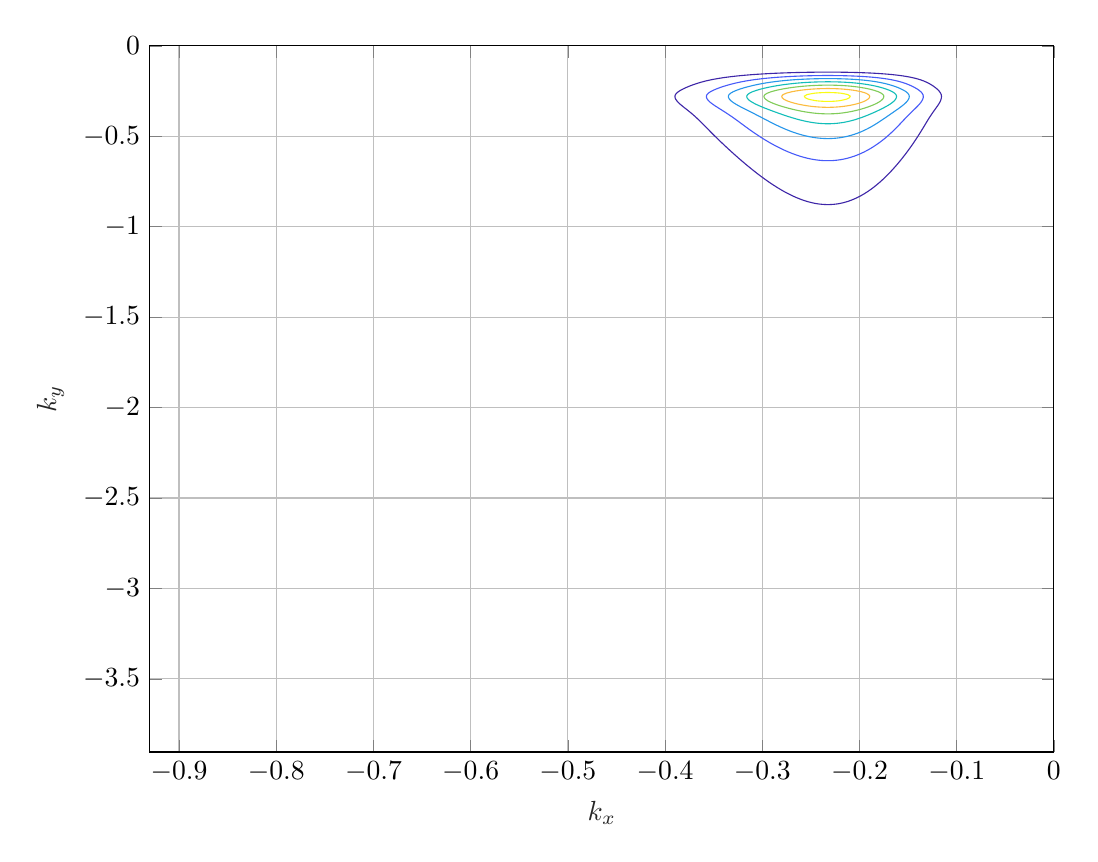
\begin{tikzpicture}

\begin{axis}[%
width=4.521in,
height=3.531in,
at={(0.758in,0.516in)},
scale only axis,
colormap={mymap}{[1pt] rgb(0pt)=(0.2422,0.1504,0.6603); rgb(1pt)=(0.2444,0.1534,0.6728); rgb(2pt)=(0.2464,0.1569,0.6847); rgb(3pt)=(0.2484,0.1607,0.6961); rgb(4pt)=(0.2503,0.1648,0.7071); rgb(5pt)=(0.2522,0.1689,0.7179); rgb(6pt)=(0.254,0.1732,0.7286); rgb(7pt)=(0.2558,0.1773,0.7393); rgb(8pt)=(0.2576,0.1814,0.7501); rgb(9pt)=(0.2594,0.1854,0.761); rgb(11pt)=(0.2628,0.1932,0.7828); rgb(12pt)=(0.2645,0.1972,0.7937); rgb(13pt)=(0.2661,0.2011,0.8043); rgb(14pt)=(0.2676,0.2052,0.8148); rgb(15pt)=(0.2691,0.2094,0.8249); rgb(16pt)=(0.2704,0.2138,0.8346); rgb(17pt)=(0.2717,0.2184,0.8439); rgb(18pt)=(0.2729,0.2231,0.8528); rgb(19pt)=(0.274,0.228,0.8612); rgb(20pt)=(0.2749,0.233,0.8692); rgb(21pt)=(0.2758,0.2382,0.8767); rgb(22pt)=(0.2766,0.2435,0.884); rgb(23pt)=(0.2774,0.2489,0.8908); rgb(24pt)=(0.2781,0.2543,0.8973); rgb(25pt)=(0.2788,0.2598,0.9035); rgb(26pt)=(0.2794,0.2653,0.9094); rgb(27pt)=(0.2798,0.2708,0.915); rgb(28pt)=(0.2802,0.2764,0.9204); rgb(29pt)=(0.2806,0.2819,0.9255); rgb(30pt)=(0.2809,0.2875,0.9305); rgb(31pt)=(0.2811,0.293,0.9352); rgb(32pt)=(0.2813,0.2985,0.9397); rgb(33pt)=(0.2814,0.304,0.9441); rgb(34pt)=(0.2814,0.3095,0.9483); rgb(35pt)=(0.2813,0.315,0.9524); rgb(36pt)=(0.2811,0.3204,0.9563); rgb(37pt)=(0.2809,0.3259,0.96); rgb(38pt)=(0.2807,0.3313,0.9636); rgb(39pt)=(0.2803,0.3367,0.967); rgb(40pt)=(0.2798,0.3421,0.9702); rgb(41pt)=(0.2791,0.3475,0.9733); rgb(42pt)=(0.2784,0.3529,0.9763); rgb(43pt)=(0.2776,0.3583,0.9791); rgb(44pt)=(0.2766,0.3638,0.9817); rgb(45pt)=(0.2754,0.3693,0.984); rgb(46pt)=(0.2741,0.3748,0.9862); rgb(47pt)=(0.2726,0.3804,0.9881); rgb(48pt)=(0.271,0.386,0.9898); rgb(49pt)=(0.2691,0.3916,0.9912); rgb(50pt)=(0.267,0.3973,0.9924); rgb(51pt)=(0.2647,0.403,0.9935); rgb(52pt)=(0.2621,0.4088,0.9946); rgb(53pt)=(0.2591,0.4145,0.9955); rgb(54pt)=(0.2556,0.4203,0.9965); rgb(55pt)=(0.2517,0.4261,0.9974); rgb(56pt)=(0.2473,0.4319,0.9983); rgb(57pt)=(0.2424,0.4378,0.9991); rgb(58pt)=(0.2369,0.4437,0.9996); rgb(59pt)=(0.2311,0.4497,0.9995); rgb(60pt)=(0.225,0.4559,0.9985); rgb(61pt)=(0.2189,0.462,0.9968); rgb(62pt)=(0.2128,0.4682,0.9948); rgb(63pt)=(0.2066,0.4743,0.9926); rgb(64pt)=(0.2006,0.4803,0.9906); rgb(65pt)=(0.195,0.4861,0.9887); rgb(66pt)=(0.1903,0.4919,0.9867); rgb(67pt)=(0.1869,0.4975,0.9844); rgb(68pt)=(0.1847,0.503,0.9819); rgb(69pt)=(0.1831,0.5084,0.9793); rgb(70pt)=(0.1818,0.5138,0.9766); rgb(71pt)=(0.1806,0.5191,0.9738); rgb(72pt)=(0.1795,0.5244,0.9709); rgb(73pt)=(0.1785,0.5296,0.9677); rgb(74pt)=(0.1778,0.5349,0.9641); rgb(75pt)=(0.1773,0.5401,0.9602); rgb(76pt)=(0.1768,0.5452,0.956); rgb(77pt)=(0.1764,0.5504,0.9516); rgb(78pt)=(0.1755,0.5554,0.9473); rgb(79pt)=(0.174,0.5605,0.9432); rgb(80pt)=(0.1716,0.5655,0.9393); rgb(81pt)=(0.1686,0.5705,0.9357); rgb(82pt)=(0.1649,0.5755,0.9323); rgb(83pt)=(0.161,0.5805,0.9289); rgb(84pt)=(0.1573,0.5854,0.9254); rgb(85pt)=(0.154,0.5902,0.9218); rgb(86pt)=(0.1513,0.595,0.9182); rgb(87pt)=(0.1492,0.5997,0.9147); rgb(88pt)=(0.1475,0.6043,0.9113); rgb(89pt)=(0.1461,0.6089,0.908); rgb(90pt)=(0.1446,0.6135,0.905); rgb(91pt)=(0.1429,0.618,0.9022); rgb(92pt)=(0.1408,0.6226,0.8998); rgb(93pt)=(0.1383,0.6272,0.8975); rgb(94pt)=(0.1354,0.6317,0.8953); rgb(95pt)=(0.1321,0.6363,0.8932); rgb(96pt)=(0.1288,0.6408,0.891); rgb(97pt)=(0.1253,0.6453,0.8887); rgb(98pt)=(0.1219,0.6497,0.8862); rgb(99pt)=(0.1185,0.6541,0.8834); rgb(100pt)=(0.1152,0.6584,0.8804); rgb(101pt)=(0.1119,0.6627,0.877); rgb(102pt)=(0.1085,0.6669,0.8734); rgb(103pt)=(0.1048,0.671,0.8695); rgb(104pt)=(0.1009,0.675,0.8653); rgb(105pt)=(0.0964,0.6789,0.8609); rgb(106pt)=(0.0914,0.6828,0.8562); rgb(107pt)=(0.0855,0.6865,0.8513); rgb(108pt)=(0.0789,0.6902,0.8462); rgb(109pt)=(0.0713,0.6938,0.8409); rgb(110pt)=(0.0628,0.6972,0.8355); rgb(111pt)=(0.0535,0.7006,0.8299); rgb(112pt)=(0.0433,0.7039,0.8242); rgb(113pt)=(0.0328,0.7071,0.8183); rgb(114pt)=(0.0234,0.7103,0.8124); rgb(115pt)=(0.0155,0.7133,0.8064); rgb(116pt)=(0.0091,0.7163,0.8003); rgb(117pt)=(0.0046,0.7192,0.7941); rgb(118pt)=(0.0019,0.722,0.7878); rgb(119pt)=(0.0009,0.7248,0.7815); rgb(120pt)=(0.0018,0.7275,0.7752); rgb(121pt)=(0.0046,0.7301,0.7688); rgb(122pt)=(0.0094,0.7327,0.7623); rgb(123pt)=(0.0162,0.7352,0.7558); rgb(124pt)=(0.0253,0.7376,0.7492); rgb(125pt)=(0.0369,0.74,0.7426); rgb(126pt)=(0.0504,0.7423,0.7359); rgb(127pt)=(0.0638,0.7446,0.7292); rgb(128pt)=(0.077,0.7468,0.7224); rgb(129pt)=(0.0899,0.7489,0.7156); rgb(130pt)=(0.1023,0.751,0.7088); rgb(131pt)=(0.1141,0.7531,0.7019); rgb(132pt)=(0.1252,0.7552,0.695); rgb(133pt)=(0.1354,0.7572,0.6881); rgb(134pt)=(0.1448,0.7593,0.6812); rgb(135pt)=(0.1532,0.7614,0.6741); rgb(136pt)=(0.1609,0.7635,0.6671); rgb(137pt)=(0.1678,0.7656,0.6599); rgb(138pt)=(0.1741,0.7678,0.6527); rgb(139pt)=(0.1799,0.7699,0.6454); rgb(140pt)=(0.1853,0.7721,0.6379); rgb(141pt)=(0.1905,0.7743,0.6303); rgb(142pt)=(0.1954,0.7765,0.6225); rgb(143pt)=(0.2003,0.7787,0.6146); rgb(144pt)=(0.2061,0.7808,0.6065); rgb(145pt)=(0.2118,0.7828,0.5983); rgb(146pt)=(0.2178,0.7849,0.5899); rgb(147pt)=(0.2244,0.7869,0.5813); rgb(148pt)=(0.2318,0.7887,0.5725); rgb(149pt)=(0.2401,0.7905,0.5636); rgb(150pt)=(0.2491,0.7922,0.5546); rgb(151pt)=(0.2589,0.7937,0.5454); rgb(152pt)=(0.2695,0.7951,0.536); rgb(153pt)=(0.2809,0.7964,0.5266); rgb(154pt)=(0.2929,0.7975,0.517); rgb(155pt)=(0.3052,0.7985,0.5074); rgb(156pt)=(0.3176,0.7994,0.4975); rgb(157pt)=(0.3301,0.8002,0.4876); rgb(158pt)=(0.3424,0.8009,0.4774); rgb(159pt)=(0.3548,0.8016,0.4669); rgb(160pt)=(0.3671,0.8021,0.4563); rgb(161pt)=(0.3795,0.8026,0.4454); rgb(162pt)=(0.3921,0.8029,0.4344); rgb(163pt)=(0.405,0.8031,0.4233); rgb(164pt)=(0.4184,0.803,0.4122); rgb(165pt)=(0.4322,0.8028,0.4013); rgb(166pt)=(0.4463,0.8024,0.3904); rgb(167pt)=(0.4608,0.8018,0.3797); rgb(168pt)=(0.4753,0.8011,0.3691); rgb(169pt)=(0.4899,0.8002,0.3586); rgb(170pt)=(0.5044,0.7993,0.348); rgb(171pt)=(0.5187,0.7982,0.3374); rgb(172pt)=(0.5329,0.797,0.3267); rgb(173pt)=(0.547,0.7957,0.3159); rgb(175pt)=(0.5748,0.7929,0.2941); rgb(176pt)=(0.5886,0.7913,0.2833); rgb(177pt)=(0.6024,0.7896,0.2726); rgb(178pt)=(0.6161,0.7878,0.2622); rgb(179pt)=(0.6297,0.7859,0.2521); rgb(180pt)=(0.6433,0.7839,0.2423); rgb(181pt)=(0.6567,0.7818,0.2329); rgb(182pt)=(0.6701,0.7796,0.2239); rgb(183pt)=(0.6833,0.7773,0.2155); rgb(184pt)=(0.6963,0.775,0.2075); rgb(185pt)=(0.7091,0.7727,0.1998); rgb(186pt)=(0.7218,0.7703,0.1924); rgb(187pt)=(0.7344,0.7679,0.1852); rgb(188pt)=(0.7468,0.7654,0.1782); rgb(189pt)=(0.759,0.7629,0.1717); rgb(190pt)=(0.771,0.7604,0.1658); rgb(191pt)=(0.7829,0.7579,0.1608); rgb(192pt)=(0.7945,0.7554,0.157); rgb(193pt)=(0.806,0.7529,0.1546); rgb(194pt)=(0.8172,0.7505,0.1535); rgb(195pt)=(0.8281,0.7481,0.1536); rgb(196pt)=(0.8389,0.7457,0.1546); rgb(197pt)=(0.8495,0.7435,0.1564); rgb(198pt)=(0.86,0.7413,0.1587); rgb(199pt)=(0.8703,0.7392,0.1615); rgb(200pt)=(0.8804,0.7372,0.165); rgb(201pt)=(0.8903,0.7353,0.1695); rgb(202pt)=(0.9,0.7336,0.1749); rgb(203pt)=(0.9093,0.7321,0.1815); rgb(204pt)=(0.9184,0.7308,0.189); rgb(205pt)=(0.9272,0.7298,0.1973); rgb(206pt)=(0.9357,0.729,0.2061); rgb(207pt)=(0.944,0.7285,0.2151); rgb(208pt)=(0.9523,0.7284,0.2237); rgb(209pt)=(0.9606,0.7285,0.2312); rgb(210pt)=(0.9689,0.7292,0.2373); rgb(211pt)=(0.977,0.7304,0.2418); rgb(212pt)=(0.9842,0.733,0.2446); rgb(213pt)=(0.99,0.7365,0.2429); rgb(214pt)=(0.9946,0.7407,0.2394); rgb(215pt)=(0.9966,0.7458,0.2351); rgb(216pt)=(0.9971,0.7513,0.2309); rgb(217pt)=(0.9972,0.7569,0.2267); rgb(218pt)=(0.9971,0.7626,0.2224); rgb(219pt)=(0.9969,0.7683,0.2181); rgb(220pt)=(0.9966,0.774,0.2138); rgb(221pt)=(0.9962,0.7798,0.2095); rgb(222pt)=(0.9957,0.7856,0.2053); rgb(223pt)=(0.9949,0.7915,0.2012); rgb(224pt)=(0.9938,0.7974,0.1974); rgb(225pt)=(0.9923,0.8034,0.1939); rgb(226pt)=(0.9906,0.8095,0.1906); rgb(227pt)=(0.9885,0.8156,0.1875); rgb(228pt)=(0.9861,0.8218,0.1846); rgb(229pt)=(0.9835,0.828,0.1817); rgb(230pt)=(0.9807,0.8342,0.1787); rgb(231pt)=(0.9778,0.8404,0.1757); rgb(232pt)=(0.9748,0.8467,0.1726); rgb(233pt)=(0.972,0.8529,0.1695); rgb(234pt)=(0.9694,0.8591,0.1665); rgb(235pt)=(0.9671,0.8654,0.1636); rgb(236pt)=(0.9651,0.8716,0.1608); rgb(237pt)=(0.9634,0.8778,0.1582); rgb(238pt)=(0.9619,0.884,0.1557); rgb(239pt)=(0.9608,0.8902,0.1532); rgb(240pt)=(0.9601,0.8963,0.1507); rgb(241pt)=(0.9596,0.9023,0.148); rgb(242pt)=(0.9595,0.9084,0.145); rgb(243pt)=(0.9597,0.9143,0.1418); rgb(244pt)=(0.9601,0.9203,0.1382); rgb(245pt)=(0.9608,0.9262,0.1344); rgb(246pt)=(0.9618,0.932,0.1304); rgb(247pt)=(0.9629,0.9379,0.1261); rgb(248pt)=(0.9642,0.9437,0.1216); rgb(249pt)=(0.9657,0.9494,0.1168); rgb(250pt)=(0.9674,0.9552,0.1116); rgb(251pt)=(0.9692,0.9609,0.1061); rgb(252pt)=(0.9711,0.9667,0.1001); rgb(253pt)=(0.973,0.9724,0.0938); rgb(254pt)=(0.9749,0.9782,0.0872); rgb(255pt)=(0.9769,0.9839,0.0805)},
xmin=-0.930195154145727,
xmax=0,
xlabel style={font=\color{white!15!black}},
xlabel={$k_{x}$},
ymin=-3.90455241197714,
ymax=0,
ylabel style={font=\color{white!15!black}},
ylabel={$k_{y}$},
axis background/.style={fill=white},
xmajorgrids,
ymajorgrids
]
\addplot[contour prepared, contour prepared format=matlab, contour/labels=false] table[row sep=crcr] {%
%
0.005	291\\
-0.196855524076637	-0.148804468836322\\
-0.198674719356596	-0.148433867867508\\
-0.202114910320485	-0.147817601337958\\
-0.205584630820544	-0.147283319880835\\
-0.209083880856774	-0.146826004027864\\
-0.212612660429175	-0.14644142234799\\
-0.216170969537747	-0.146126063608075\\
-0.219758808182489	-0.145877081252974\\
-0.223376176363402	-0.145692248928751\\
-0.227023074080486	-0.14556992603921\\
-0.230699501333741	-0.145509032561826\\
-0.234405458123166	-0.145509032561826\\
-0.238140944448762	-0.14556992603921\\
-0.241905960310528	-0.145692248928751\\
-0.245700505708466	-0.145877081252974\\
-0.249524580642574	-0.146126063608075\\
-0.253378185112853	-0.14644142234799\\
-0.257261319119302	-0.146826004027864\\
-0.261173982661922	-0.147283319880835\\
-0.265116175740713	-0.147817601337958\\
-0.269087898355675	-0.148433867867508\\
-0.271222105805323	-0.148804468836322\\
-0.273089150506807	-0.149104807550245\\
-0.27711993219411	-0.149824158172332\\
-0.281180243417584	-0.150635959419721\\
-0.285270084177229	-0.151548459180424\\
-0.289389454473044	-0.152571149054126\\
-0.29353835430503	-0.153714935316677\\
-0.297553240260792	-0.154940096664225\\
-0.297716783673187	-0.154988697633428\\
-0.301924742577514	-0.156314715300856\\
-0.306162231018012	-0.157793763577976\\
-0.310429248994681	-0.159443486906332\\
-0.31453911910122	-0.16119967656946\\
-0.314725796507521	-0.161280562510135\\
-0.319051873556531	-0.163247627065405\\
-0.323407480141712	-0.16544565909229\\
-0.327252114451645	-0.167583208552026\\
-0.327792616263064	-0.167898317448867\\
-0.332207281920586	-0.170599691153822\\
-0.33665147711428	-0.173629918284633\\
-0.337297872466221	-0.174090692611923\\
-0.341125201844143	-0.177036387569275\\
-0.345466534960891	-0.180722128749152\\
-0.345628456110178	-0.180873221784687\\
-0.350161239912383	-0.185264112153009\\
-0.352293310357913	-0.187477516963712\\
-0.354723553250759	-0.190291912618386\\
-0.35805050675298	-0.194356857255604\\
-0.359315396125306	-0.196089116464486\\
-0.363021647798467	-0.201360149624827\\
-0.363936768536024	-0.202816600288493\\
-0.367413526580762	-0.208487394071381\\
-0.368587670482912	-0.210618769986536\\
-0.371370269485799	-0.215738590595267\\
-0.373268101965971	-0.219607025448017\\
-0.374981450526961	-0.223113739196484\\
-0.3779780629852	-0.229926330649419\\
-0.378281417689195	-0.230612839875033\\
-0.381359513645215	-0.238235892630913\\
-0.382717553540601	-0.242136385597928\\
-0.384083624628014	-0.245982897464124\\
-0.386390104929891	-0.253853854374666\\
-0.387486573632172	-0.258852020168781\\
-0.388173452577456	-0.26184876336254\\
-0.389377043294675	-0.269967624427746\\
-0.389874749315474	-0.278210437570283\\
-0.389729844221555	-0.286577202790151\\
-0.389096914997133	-0.29506792008735\\
-0.388009499636901	-0.303682589461881\\
-0.387486573632172	-0.306788620687696\\
-0.386586484665742	-0.312421210913744\\
-0.384868963598134	-0.321283784442937\\
-0.382866623338682	-0.330270310049462\\
-0.382717553540601	-0.330906931919109\\
-0.380799600534545	-0.339380787733319\\
-0.378589148207348	-0.348615217494507\\
-0.3779780629852	-0.35117471046037\\
-0.376400913254779	-0.357973599333026\\
-0.374201037837619	-0.367455933248876\\
-0.373268101965971	-0.371586176913506\\
-0.372064534739705	-0.377062219242058\\
-0.369983893974356	-0.386792457312572\\
-0.368587670482912	-0.393481854733007\\
-0.367944571306966	-0.396646647460416\\
-0.365990433558918	-0.406624789685592\\
-0.364018526546915	-0.4167268839881\\
-0.363936768536024	-0.417159908765357\\
-0.362135868686593	-0.426952930367939\\
-0.360214540699268	-0.437302928825109\\
-0.359315396125306	-0.442158660529871\\
-0.358298790518745	-0.447776879359611\\
-0.3563690199839	-0.458374781971444\\
-0.354723553250759	-0.467221757102483\\
-0.354381364869922	-0.469096636660608\\
-0.352401999488538	-0.479942443427104\\
-0.350333380855871	-0.490912202270931\\
-0.350161239912383	-0.491826386211798\\
-0.348271022203739	-0.502005913192089\\
-0.34612242741626	-0.513223576190579\\
-0.345628456110178	-0.515792438892124\\
-0.343956898785391	-0.524565191266401\\
-0.341716641755384	-0.536030758419553\\
-0.341125201844143	-0.539045030714727\\
-0.339449944008873	-0.547620277650037\\
-0.337108764257676	-0.559333748957853\\
-0.33665147711428	-0.561620832228334\\
-0.334741187145012	-0.571171172343\\
-0.332289664043878	-0.583132547805478\\
-0.332207281920586	-0.583537339335937\\
-0.329817841011296	-0.595217875345287\\
-0.327792616263064	-0.604909596975648\\
-0.327261323684509	-0.607427154962428\\
-0.324661100549576	-0.6197603866569\\
-0.323407480141712	-0.625653932759719\\
-0.321990651064844	-0.632217570428704\\
-0.319244792399452	-0.644798706277839\\
-0.319051873556531	-0.645689511016548\\
-0.316442612535861	-0.657503794204306\\
-0.314725796507521	-0.66519911681604\\
-0.31355182540106	-0.670332834208104\\
-0.310575062176663	-0.683285826289233\\
-0.310429248994681	-0.683926322226188\\
-0.307512020708161	-0.696362770447694\\
-0.306162231018012	-0.702096889863331\\
-0.304341183342933	-0.709563666683486\\
-0.301924742577514	-0.719467560925802\\
-0.301054927994755	-0.722888514996609\\
-0.297716783673187	-0.73605183071751\\
-0.297640872845205	-0.736337315387063\\
-0.29407261737457	-0.74991006785485\\
-0.29353835430503	-0.751955516225179\\
-0.290326752974816	-0.763606772399967\\
-0.289389454473044	-0.767036452644243\\
-0.286371311032162	-0.777427429022416\\
-0.285270084177229	-0.781262510564789\\
-0.282160893471094	-0.791372037722196\\
-0.281180243417584	-0.794606641339117\\
-0.277632131274088	-0.805440598499308\\
-0.27711993219411	-0.807031638078997\\
-0.273089150506807	-0.818546853252477\\
-0.272671653302337	-0.819633111353751\\
-0.269087898355675	-0.829172796395043\\
-0.267084087910637	-0.833949576285525\\
-0.265116175740713	-0.838762426158114\\
-0.261173982661922	-0.847293473774731\\
-0.260596261761032	-0.848389993294631\\
-0.257261319119302	-0.854920297723456\\
-0.253378185112853	-0.861382357862224\\
-0.252246285753978	-0.862954362381068\\
-0.249524580642574	-0.866875807813234\\
-0.245700505708466	-0.871277784427371\\
-0.241905960310528	-0.874545596591965\\
-0.238140944448762	-0.876708249840691\\
-0.234899910151014	-0.877642683544837\\
-0.234405458123166	-0.877792238657428\\
-0.230699501333741	-0.877792238657428\\
-0.230212866729258	-0.877642683544837\\
-0.227023074080486	-0.876708249840691\\
-0.223376176363402	-0.874545596591965\\
-0.219758808182489	-0.871277784427371\\
-0.216170969537747	-0.866875807813234\\
-0.213657824204994	-0.862954362381068\\
-0.212612660429175	-0.861382357862224\\
-0.209083880856774	-0.854920297723456\\
-0.206101309513038	-0.848389993294631\\
-0.205584630820544	-0.847293473774731\\
-0.202114910320485	-0.838762426158114\\
-0.200410361861034	-0.833949576285525\\
-0.198674719356596	-0.829172796395043\\
-0.195619931929736	-0.819633111353751\\
-0.195264057928878	-0.818546853252477\\
-0.191882926037331	-0.807031638078997\\
-0.191460128978586	-0.805440598499308\\
-0.188531323681954	-0.794606641339117\\
-0.187734766779284	-0.791372037722196\\
-0.185209250862748	-0.781262510564789\\
-0.184329058788734	-0.777427429022416\\
-0.181916707579713	-0.767036452644242\\
-0.181179543989352	-0.763606772399967\\
-0.178653693832849	-0.751955516225179\\
-0.17824025350695	-0.74991006785485\\
-0.175478953337095	-0.736337315387063\\
-0.175420209622155	-0.73605183071751\\
-0.172878534822926	-0.722888514996609\\
-0.172216254947632	-0.719467560925802\\
-0.170406029287127	-0.709563666683486\\
-0.16904182980928	-0.702096889863331\\
-0.168047002113772	-0.696362770447694\\
-0.165896934207098	-0.683926322226188\\
-0.165791207123256	-0.683285826289233\\
-0.163632798049896	-0.670332834208104\\
-0.162781568141087	-0.66519911681604\\
-0.161556945103807	-0.657503794204306\\
-0.159695731611247	-0.645689511016547\\
-0.159560361440113	-0.644798706277839\\
-0.157633606376601	-0.632217570428704\\
-0.156639424617578	-0.625653932759718\\
-0.155774131070062	-0.6197603866569\\
-0.153979364259755	-0.607427154962428\\
-0.153612647160079	-0.604909596975648\\
-0.152237661795895	-0.595217875345287\\
-0.150615399238751	-0.583537339335937\\
-0.150560386591636	-0.583132547805478\\
-0.14892332299254	-0.571171172343\\
-0.147647680853594	-0.561620832228333\\
-0.147347350353475	-0.559333748957853\\
-0.145809743850214	-0.547620277650037\\
-0.144709492004607	-0.539045030714727\\
-0.144327479996363	-0.536030758419553\\
-0.14288049430813	-0.524565191266401\\
-0.141800832691792	-0.515792438892124\\
-0.141487072415941	-0.513223576190579\\
-0.140122329798488	-0.502005913192089\\
-0.138921702915147	-0.491826386211798\\
-0.138814184461771	-0.490912202270931\\
-0.137522134636189	-0.479942443427104\\
-0.136285831986976	-0.469096636660608\\
-0.136072102674672	-0.467221757102482\\
-0.135061542719593	-0.458374781971444\\
-0.1338763781789	-0.447776879359611\\
-0.133252031970369	-0.442158660529871\\
-0.132709098026347	-0.437302928825109\\
-0.131548935120263	-0.426952930367939\\
-0.130461490802236	-0.417159908765357\\
-0.130412955094183	-0.4167268839881\\
-0.129242330931502	-0.406624789685592\\
-0.12808225550647	-0.396646647460416\\
-0.127700479170273	-0.393481854733007\\
-0.126885648426055	-0.386792457312572\\
-0.12567139435164	-0.377062219242058\\
-0.124968997074482	-0.371586176913505\\
-0.124433801887925	-0.367455933248876\\
-0.123171804391561	-0.357973599333026\\
-0.122267044514861	-0.35117471046037\\
-0.121922476212031	-0.348615217494507\\
-0.120676084089842	-0.339380787733319\\
-0.119594621491411	-0.330906931919108\\
-0.119512010055323	-0.330270310049462\\
-0.118402353998227	-0.321283784442937\\
-0.117450538917417	-0.312421210913744\\
-0.116951728004132	-0.306788620687696\\
-0.116666934456941	-0.303682589461881\\
-0.116074711322292	-0.29506792008735\\
-0.115730008329299	-0.286577202790151\\
-0.115651090785841	-0.278210437570283\\
-0.115922149141784	-0.269967624427746\\
-0.116577643163162	-0.26184876336254\\
-0.116951728004132	-0.258852020168781\\
-0.117559368554313	-0.253853854374666\\
-0.118837572808294	-0.245982897464124\\
-0.119594621491411	-0.242136385597929\\
-0.120360369843638	-0.238235892630913\\
-0.122095994043138	-0.230612839875033\\
-0.122267044514861	-0.229926330649419\\
-0.123986104326328	-0.223113739196484\\
-0.124968997074482	-0.219607025448017\\
-0.126076564925686	-0.215738590595267\\
-0.127700479170273	-0.210618769986537\\
-0.128397510629645	-0.208487394071381\\
-0.130461490802236	-0.202816600288493\\
-0.131014071694882	-0.201360149624827\\
-0.133252031970369	-0.196089116464486\\
-0.134028861134723	-0.194356857255604\\
-0.136072102674672	-0.190291912618386\\
-0.137590021374735	-0.187477516963712\\
-0.138921702915147	-0.185264112153009\\
-0.141800832691792	-0.180873221784687\\
-0.141905417827561	-0.180722128749152\\
-0.144709492004607	-0.177036387569275\\
-0.147223150572946	-0.174090692611923\\
-0.147647680853594	-0.173629918284633\\
-0.150615399238751	-0.170599691153822\\
-0.153612647160079	-0.167898317448867\\
-0.153985720800958	-0.167583208552026\\
-0.156639424617578	-0.16544565909229\\
-0.159695731611247	-0.163247627065405\\
-0.162781568141087	-0.161280562510135\\
-0.162916925298233	-0.16119967656946\\
-0.165896934207098	-0.159443486906332\\
-0.16904182980928	-0.157793763577976\\
-0.172216254947632	-0.156314715300856\\
-0.175420209622155	-0.154988697633428\\
-0.175546767951888	-0.154940096664225\\
-0.178653693832849	-0.153714935316677\\
-0.181916707579713	-0.152571149054126\\
-0.185209250862748	-0.151548459180424\\
-0.188531323681954	-0.150635959419721\\
-0.191882926037331	-0.149824158172332\\
-0.195264057928878	-0.149104807550245\\
-0.196855524076637	-0.148804468836322\\
0.01	221\\
-0.204089990128102	-0.167583208552026\\
-0.205584630820544	-0.167218882689699\\
-0.209083880856774	-0.166485513857602\\
-0.212612660429175	-0.165868784269982\\
-0.216170969537747	-0.165363063181853\\
-0.219758808182489	-0.16496378575076\\
-0.223376176363402	-0.164667381712132\\
-0.227023074080486	-0.164471220144456\\
-0.230699501333741	-0.164373569083158\\
-0.234405458123166	-0.164373569083158\\
-0.238140944448762	-0.164471220144456\\
-0.241905960310528	-0.164667381712132\\
-0.245700505708466	-0.16496378575076\\
-0.249524580642574	-0.165363063181853\\
-0.253378185112853	-0.165868784269982\\
-0.257261319119302	-0.166485513857602\\
-0.261173982661922	-0.167218882689699\\
-0.262872148895463	-0.167583208552026\\
-0.265116175740713	-0.168066252699074\\
-0.269087898355675	-0.169035609526974\\
-0.273089150506807	-0.170143188319726\\
-0.27711993219411	-0.171399774174091\\
-0.281180243417584	-0.172817855889325\\
-0.284470172642135	-0.174090692611923\\
-0.285270084177229	-0.174412037444747\\
-0.289389454473044	-0.176199598422342\\
-0.29353835430503	-0.178198823937543\\
-0.297716783673187	-0.180431601456792\\
-0.298228986807371	-0.180722128749152\\
-0.301924742577514	-0.182956929066661\\
-0.306162231018012	-0.18577868227302\\
-0.308523207559827	-0.187477516963712\\
-0.310429248994681	-0.188960796527956\\
-0.314725796507521	-0.192556732638394\\
-0.316730651067302	-0.194356857255604\\
-0.319051873556531	-0.196628013938362\\
-0.323407480141712	-0.20122875595073\\
-0.323526952683711	-0.201360149624827\\
-0.327792616263064	-0.206478524097554\\
-0.329370113272455	-0.208487394071381\\
-0.332207281920586	-0.212406814423409\\
-0.334506185326786	-0.215738590595267\\
-0.33665147711428	-0.219095158965312\\
-0.339123927902316	-0.223113739196484\\
-0.341125201844143	-0.226633807786818\\
-0.343322659406662	-0.230612839875033\\
-0.345628456110178	-0.235205105959218\\
-0.34712043165907	-0.238235892630913\\
-0.350161239912383	-0.245280834883703\\
-0.350461503037606	-0.245982897464124\\
-0.353308332547513	-0.253853854374666\\
-0.354723553250759	-0.259086882558368\\
-0.355481780738441	-0.26184876336254\\
-0.356925121700895	-0.269967624427746\\
-0.357521968682848	-0.278210437570283\\
-0.357348199099277	-0.286577202790151\\
-0.356589193016167	-0.29506792008735\\
-0.355285169056718	-0.303682589461881\\
-0.354723553250759	-0.306467690681803\\
-0.353550719021274	-0.312421210913744\\
-0.351430826796234	-0.321283784442937\\
-0.350161239912383	-0.325999981810127\\
-0.349020587202476	-0.330270310049462\\
-0.346409003644198	-0.339380787733319\\
-0.345628456110178	-0.342037977169414\\
-0.343695354871991	-0.348615217494507\\
-0.341125201844143	-0.357228574374069\\
-0.340901822513782	-0.357973599333026\\
-0.338146451362843	-0.367455933248876\\
-0.33665147711428	-0.372711844083202\\
-0.335405819887601	-0.377062219242058\\
-0.332709708666971	-0.386792457312572\\
-0.332207281920586	-0.388688533497818\\
-0.330082350732401	-0.396646647460416\\
-0.327792616263064	-0.405408136891623\\
-0.327471216630879	-0.406624789685592\\
-0.324904412199593	-0.4167268839881\\
-0.323407480141712	-0.422693008355968\\
-0.322324211511001	-0.426952930367939\\
-0.31972179197521	-0.437302928825109\\
-0.319051873556531	-0.439994651252416\\
-0.317080868155977	-0.447776879359611\\
-0.314725796507521	-0.456991820026865\\
-0.314364297807172	-0.458374781971444\\
-0.311574761806662	-0.469096636660608\\
-0.310429248994681	-0.473463888399764\\
-0.308681475617418	-0.479942443427104\\
-0.306162231018012	-0.489173268075743\\
-0.305671252620898	-0.490912202270931\\
-0.302533272495481	-0.502005913192089\\
-0.301924742577514	-0.504151200529747\\
-0.299245230226036	-0.513223576190579\\
-0.297716783673187	-0.518370561666152\\
-0.295788918317463	-0.524565191266401\\
-0.29353835430503	-0.531784147201311\\
-0.29214125593058	-0.536030758419553\\
-0.289389454473044	-0.544412141696058\\
-0.288269651930774	-0.547620277650037\\
-0.285270084177229	-0.556263773426203\\
-0.28412831207742	-0.559333748957853\\
-0.281180243417584	-0.567336267190073\\
-0.279652795586088	-0.571171172343\\
-0.27711993219411	-0.577614576536799\\
-0.27475164815669	-0.583132547805478\\
-0.273089150506807	-0.587071378449766\\
-0.26929302115733	-0.595217875345287\\
-0.269087898355675	-0.595667047275528\\
-0.265116175740713	-0.603544820128684\\
-0.262897202877986	-0.607427154962428\\
-0.261173982661922	-0.610522882704594\\
-0.257261319119302	-0.616662936631505\\
-0.254947771350379	-0.6197603866569\\
-0.253378185112853	-0.621931397163592\\
-0.249524580642574	-0.626380588210412\\
-0.245700505708466	-0.629893318079344\\
-0.242321511202533	-0.632217570428704\\
-0.241905960310528	-0.632515512795357\\
-0.238140944448762	-0.634329673244236\\
-0.234405458123166	-0.635232779266986\\
-0.230699501333741	-0.635232779266986\\
-0.227023074080486	-0.634329673244236\\
-0.223376176363402	-0.632515512795357\\
-0.222980028625888	-0.632217570428704\\
-0.219758808182489	-0.629893318079344\\
-0.216170969537747	-0.626380588210412\\
-0.212612660429175	-0.621931397163592\\
-0.211186306395834	-0.6197603866569\\
-0.209083880856774	-0.616662936631505\\
-0.205584630820544	-0.610522882704594\\
-0.204067938870076	-0.607427154962428\\
-0.202114910320485	-0.603544820128684\\
-0.198674719356596	-0.595667047275528\\
-0.19849987298323	-0.595217875345287\\
-0.195264057928878	-0.587071378449766\\
-0.193869508618171	-0.583132547805478\\
-0.191882926037331	-0.577614576536799\\
-0.189792162437408	-0.571171172343\\
-0.188531323681954	-0.567336267190073\\
-0.186136683073784	-0.559333748957853\\
-0.185209250862748	-0.556263773426203\\
-0.182811746887693	-0.547620277650037\\
-0.181916707579713	-0.544412141696057\\
-0.179752479387131	-0.536030758419553\\
-0.178653693832849	-0.531784147201311\\
-0.176912091293192	-0.524565191266401\\
-0.175420209622155	-0.518370561666152\\
-0.174256445053845	-0.513223576190579\\
-0.172216254947632	-0.504151200529746\\
-0.171760387587483	-0.502005913192089\\
-0.169409635925585	-0.490912202270931\\
-0.16904182980928	-0.489173268075743\\
-0.167185085519753	-0.479942443427104\\
-0.165896934207098	-0.473463888399764\\
-0.165066339006658	-0.469096636660608\\
-0.16304368575543	-0.458374781971444\\
-0.162781568141087	-0.456991820026865\\
-0.161101670617104	-0.447776879359611\\
-0.159695731611247	-0.439994651252416\\
-0.159225653263225	-0.437302928825109\\
-0.157399548707602	-0.426952930367939\\
-0.156639424617578	-0.422693008355967\\
-0.155606188685371	-0.4167268839881\\
-0.153834488657042	-0.406624789685592\\
-0.153612647160079	-0.405408136891623\\
-0.152058078272871	-0.396646647460416\\
-0.150615399238751	-0.388688533497818\\
-0.150279891677212	-0.386792457312572\\
-0.148479498470081	-0.377062219242058\\
-0.147647680853594	-0.372711844083201\\
-0.146665833079785	-0.367455933248876\\
-0.144856199881644	-0.357973599333026\\
-0.144709492004607	-0.357228574374069\\
-0.143049425950555	-0.348615217494507\\
-0.141800832691792	-0.342037977169414\\
-0.141305045170183	-0.339380787733319\\
-0.139646221737401	-0.330270310049462\\
-0.138921702915147	-0.325999981810127\\
-0.138128724699667	-0.321283784442937\\
-0.136804649620597	-0.312421210913744\\
-0.136072102674672	-0.306467690681803\\
-0.135727187501238	-0.303682589461881\\
-0.134926323911994	-0.29506792008735\\
-0.1344601819124	-0.286577202790151\\
-0.134353461685834	-0.278210437570283\\
-0.13472001401237	-0.269967624427746\\
-0.135606438847833	-0.26184876336254\\
-0.136072102674672	-0.259086882558368\\
-0.136956043113917	-0.253853854374666\\
-0.138734159927548	-0.245982897464124\\
-0.138921702915147	-0.245280834883704\\
-0.140853160926209	-0.238235892630913\\
-0.141800832691792	-0.235205105959218\\
-0.143290150562587	-0.230612839875033\\
-0.144709492004607	-0.226633807786818\\
-0.146023860039009	-0.223113739196484\\
-0.147647680853594	-0.219095158965312\\
-0.149080251117003	-0.215738590595267\\
-0.150615399238751	-0.212406814423409\\
-0.152541637484807	-0.208487394071381\\
-0.153612647160079	-0.206478524097554\\
-0.156556960405087	-0.201360149624827\\
-0.156639424617578	-0.20122875595073\\
-0.159695731611247	-0.196628013938362\\
-0.161351484171824	-0.194356857255604\\
-0.162781568141087	-0.192556732638394\\
-0.165896934207098	-0.188960796527956\\
-0.167301732911679	-0.187477516963712\\
-0.16904182980928	-0.18577868227302\\
-0.172216254947632	-0.182956929066661\\
-0.175030216358583	-0.180722128749152\\
-0.175420209622155	-0.180431601456792\\
-0.178653693832849	-0.178198823937543\\
-0.181916707579713	-0.176199598422342\\
-0.185209250862748	-0.174412037444747\\
-0.185858998499558	-0.174090692611923\\
-0.188531323681954	-0.172817855889325\\
-0.191882926037331	-0.171399774174091\\
-0.195264057928878	-0.170143188319726\\
-0.198674719356596	-0.169035609526974\\
-0.202114910320485	-0.168066252699074\\
-0.204089990128102	-0.167583208552026\\
0.015	173\\
-0.200806596518139	-0.187477516963712\\
-0.202114910320485	-0.186924544936955\\
-0.205584630820544	-0.185643764417515\\
-0.209083880856774	-0.184547485989904\\
-0.212612660429175	-0.183625566059597\\
-0.216170969537747	-0.182869587491871\\
-0.219758808182489	-0.182272726519353\\
-0.223376176363402	-0.181829646122173\\
-0.227023074080486	-0.18153641346003\\
-0.230699501333741	-0.181390439500885\\
-0.234405458123166	-0.181390439500885\\
-0.238140944448762	-0.18153641346003\\
-0.241905960310528	-0.181829646122173\\
-0.245700505708466	-0.182272726519353\\
-0.249524580642574	-0.182869587491871\\
-0.253378185112853	-0.183625566059597\\
-0.257261319119302	-0.184547485989904\\
-0.261173982661922	-0.185643764417515\\
-0.265116175740713	-0.186924544936955\\
-0.266626632448143	-0.187477516963712\\
-0.269087898355675	-0.188424031362211\\
-0.273089150506807	-0.190152486433183\\
-0.27711993219411	-0.192113477566544\\
-0.281180243417584	-0.194326494417163\\
-0.281232023051579	-0.194356857255604\\
-0.285270084177229	-0.196876836120384\\
-0.289389454473044	-0.199736017627982\\
-0.29154108648535	-0.201360149624827\\
-0.29353835430503	-0.20296613342925\\
-0.297716783673187	-0.206610918630126\\
-0.29970930286236	-0.208487394071381\\
-0.301924742577514	-0.210703450941443\\
-0.306162231018012	-0.215292633685827\\
-0.306552955041759	-0.215738590595267\\
-0.310429248994681	-0.220428372254625\\
-0.31250388305249	-0.223113739196484\\
-0.314725796507521	-0.226169299056331\\
-0.317776146884247	-0.230612839875033\\
-0.319051873556531	-0.232619287280924\\
-0.322457070581489	-0.238235892630913\\
-0.323407480141712	-0.239990642765517\\
-0.326537211925288	-0.245982897464124\\
-0.327792616263064	-0.248849373614177\\
-0.329934664004851	-0.253853854374666\\
-0.332207281920586	-0.260881651430764\\
-0.332517865951021	-0.26184876336254\\
-0.334221894446989	-0.269967624427746\\
-0.334926540328618	-0.278210437570283\\
-0.33472138553163	-0.286577202790151\\
-0.333825292350686	-0.29506792008735\\
-0.332285743453973	-0.303682589461881\\
-0.332207281920586	-0.304015211228586\\
-0.330227176635983	-0.312421210913744\\
-0.327792616263064	-0.320871093620102\\
-0.327672530488905	-0.321283784442937\\
-0.324777864422751	-0.330270310049462\\
-0.323407480141712	-0.334249765309064\\
-0.32160087481259	-0.339380787733319\\
-0.319051873556531	-0.346426602342789\\
-0.318237326506687	-0.348615217494507\\
-0.314768250215996	-0.357973599333026\\
-0.314725796507521	-0.358092045392337\\
-0.311259294581549	-0.367455933248876\\
-0.310429248994681	-0.369779918511418\\
-0.307732666825044	-0.377062219242058\\
-0.306162231018012	-0.381490202134391\\
-0.304205178335486	-0.386792457312572\\
-0.301924742577514	-0.393254845263331\\
-0.300673962484034	-0.396646647460416\\
-0.297716783673187	-0.405014759657316\\
-0.29711939683823	-0.406624789685592\\
-0.29353835430503	-0.416645964465345\\
-0.293507827366014	-0.4167268839881\\
-0.289784484905512	-0.426952930367939\\
-0.289389454473044	-0.428063026580896\\
-0.285898310037783	-0.437302928825109\\
-0.285270084177229	-0.438995475089166\\
-0.281783066521443	-0.447776879359611\\
-0.281180243417584	-0.449317309479739\\
-0.277355525330051	-0.458374781971444\\
-0.27711993219411	-0.458940090718023\\
-0.273089150506807	-0.467855652233304\\
-0.272472227573532	-0.469096636660608\\
-0.269087898355675	-0.476015431972419\\
-0.266944064510422	-0.479942443427104\\
-0.265116175740713	-0.483350096399213\\
-0.261173982661922	-0.489858908562657\\
-0.260446061607413	-0.490912202270931\\
-0.257261319119302	-0.49562667722122\\
-0.253378185112853	-0.50051564751415\\
-0.251958372701121	-0.502005913192089\\
-0.249524580642574	-0.504634599063844\\
-0.245700505708466	-0.507937971139134\\
-0.241905960310528	-0.510390233020114\\
-0.238140944448762	-0.512013151308102\\
-0.234405458123166	-0.512821055196217\\
-0.230699501333741	-0.512821055196217\\
-0.227023074080486	-0.512013151308102\\
-0.223376176363402	-0.510390233020114\\
-0.219758808182489	-0.507937971139134\\
-0.216170969537747	-0.504634599063843\\
-0.213923674954951	-0.502005913192089\\
-0.212612660429175	-0.50051564751415\\
-0.209083880856774	-0.49562667722122\\
-0.206235639461747	-0.490912202270931\\
-0.205584630820544	-0.489858908562657\\
-0.202114910320485	-0.483350096399213\\
-0.200531646070142	-0.479942443427104\\
-0.198674719356596	-0.476015431972419\\
-0.195789922126615	-0.469096636660608\\
-0.195264057928878	-0.467855652233304\\
-0.191882926037331	-0.458940090718023\\
-0.191688454612391	-0.458374781971444\\
-0.188531323681954	-0.449317309479739\\
-0.188041665926112	-0.447776879359611\\
-0.185209250862748	-0.438995475089166\\
-0.184707120515424	-0.437302928825109\\
-0.181916707579713	-0.428063026580896\\
-0.181606025282292	-0.426952930367939\\
-0.178677702564246	-0.4167268839881\\
-0.178653693832849	-0.416645964465345\\
-0.175882498374295	-0.406624789685592\\
-0.175420209622155	-0.405014759657316\\
-0.17316860329951	-0.396646647460416\\
-0.172216254947632	-0.393254845263331\\
-0.170507914571451	-0.386792457312572\\
-0.16904182980928	-0.381490202134391\\
-0.16788438058126	-0.377062219242058\\
-0.165896934207098	-0.369779918511418\\
-0.16529507984686	-0.367455933248876\\
-0.162781568141087	-0.358092045392337\\
-0.162751285461663	-0.357973599333026\\
-0.160276756639976	-0.348615217494507\\
-0.159695731611247	-0.346426602342789\\
-0.157907110390894	-0.339380787733319\\
-0.156639424617578	-0.334249765309064\\
-0.155693536477467	-0.330270310049462\\
-0.153695534647293	-0.321283784442937\\
-0.153612647160079	-0.320871093620102\\
-0.151959751656057	-0.312421210913744\\
-0.150615399238751	-0.304015211228586\\
-0.150563004659978	-0.303682589461881\\
-0.14953493380204	-0.29506792008735\\
-0.148936545996825	-0.286577202790151\\
-0.1487995489397	-0.278210437570283\\
-0.149270093199526	-0.269967624427746\\
-0.150407999271584	-0.26184876336254\\
-0.150615399238751	-0.260881651430764\\
-0.15215834718823	-0.253853854374666\\
-0.153612647160079	-0.248849373614177\\
-0.154479172039689	-0.245982897464124\\
-0.156639424617578	-0.239990642765517\\
-0.157306322173396	-0.238235892630913\\
-0.159695731611247	-0.232619287280924\\
-0.160605720944037	-0.230612839875033\\
-0.162781568141087	-0.226169299056331\\
-0.16439264628202	-0.223113739196484\\
-0.165896934207098	-0.220428372254625\\
-0.168753856739875	-0.215738590595267\\
-0.16904182980928	-0.215292633685827\\
-0.172216254947632	-0.210703450941443\\
-0.173903098520224	-0.208487394071381\\
-0.175420209622155	-0.206610918630126\\
-0.178653693832849	-0.20296613342925\\
-0.180224498772882	-0.201360149624827\\
-0.181916707579713	-0.199736017627982\\
-0.185209250862748	-0.196876836120384\\
-0.188489264412464	-0.194356857255604\\
-0.188531323681954	-0.194326494417163\\
-0.191882926037331	-0.192113477566544\\
-0.195264057928878	-0.190152486433183\\
-0.198674719356596	-0.188424031362211\\
-0.200806596518139	-0.187477516963712\\
0.02	139\\
-0.215137799195968	-0.201360149624827\\
-0.216170969537747	-0.201055872903282\\
-0.219758808182489	-0.200220137832385\\
-0.223376176363402	-0.199599728986439\\
-0.227023074080486	-0.19918913953434\\
-0.230699501333741	-0.198984744268587\\
-0.234405458123166	-0.198984744268587\\
-0.238140944448762	-0.19918913953434\\
-0.241905960310528	-0.199599728986439\\
-0.245700505708466	-0.200220137832385\\
-0.249524580642574	-0.201055872903282\\
-0.250643491261679	-0.201360149624827\\
-0.253378185112853	-0.202129927279943\\
-0.257261319119302	-0.203447377687883\\
-0.261173982661922	-0.205013991462237\\
-0.265116175740713	-0.20684426409476\\
-0.268224801831597	-0.208487394071381\\
-0.269087898355675	-0.208960834556365\\
-0.273089150506807	-0.211401048772474\\
-0.27711993219411	-0.214169554891991\\
-0.279193663924761	-0.215738590595267\\
-0.281180243417584	-0.217299521838457\\
-0.285270084177229	-0.220824151394784\\
-0.287697636321962	-0.223113739196484\\
-0.289389454473044	-0.224779239068886\\
-0.29353835430503	-0.229210105690629\\
-0.294762031345597	-0.230612839875033\\
-0.297716783673187	-0.234215731194853\\
-0.300773015649049	-0.238235892630913\\
-0.301924742577514	-0.239906488270036\\
-0.305857060064278	-0.245982897464124\\
-0.306162231018012	-0.246536851374524\\
-0.310001235670234	-0.253853854374666\\
-0.310429248994681	-0.254917363928781\\
-0.313131458242229	-0.26184876336254\\
-0.314725796507521	-0.268266279401255\\
-0.315143237265334	-0.269967624427746\\
-0.315985120792274	-0.278210437570283\\
-0.315740009810204	-0.286577202790151\\
-0.314725796507521	-0.294626771351508\\
-0.314670233355787	-0.29506792008735\\
-0.312858261738131	-0.303682589461881\\
-0.310429248994681	-0.312165170132298\\
-0.310354187581503	-0.312421210913744\\
-0.307267299105819	-0.321283784442937\\
-0.306162231018012	-0.324129023300892\\
-0.303678640495373	-0.330270310049462\\
-0.301924742577514	-0.334380868837949\\
-0.299683932753385	-0.339380787733319\\
-0.297716783673187	-0.343717133961513\\
-0.295365456693589	-0.348615217494507\\
-0.29353835430503	-0.352491612001544\\
-0.290786001164932	-0.357973599333026\\
-0.289389454473044	-0.360868040273068\\
-0.28598259271957	-0.367455933248876\\
-0.285270084177229	-0.36890954391261\\
-0.281180243417584	-0.376660705418497\\
-0.280951312923443	-0.377062219242058\\
-0.27711993219411	-0.384223629049081\\
-0.275612857029542	-0.386792457312572\\
-0.273089150506807	-0.391384751641412\\
-0.269888682092611	-0.396646647460416\\
-0.269087898355675	-0.398048747581559\\
-0.265116175740713	-0.404321431981825\\
-0.263468222667355	-0.406624789685592\\
-0.261173982661922	-0.410032203069961\\
-0.257261319119302	-0.415091738221031\\
-0.255784579801413	-0.4167268839881\\
-0.253378185112853	-0.419548664208122\\
-0.249524580642574	-0.423306798272783\\
-0.245700505708466	-0.426273924125879\\
-0.244537613046369	-0.426952930367939\\
-0.241905960310528	-0.428579619378918\\
-0.238140944448762	-0.430135930686277\\
-0.234405458123166	-0.430910676997067\\
-0.230699501333741	-0.430910676997067\\
-0.227023074080486	-0.430135930686277\\
-0.223376176363402	-0.428579619378918\\
-0.220867402354527	-0.426952930367939\\
-0.219758808182489	-0.426273924125879\\
-0.216170969537747	-0.423306798272783\\
-0.212612660429175	-0.419548664208122\\
-0.210425860693184	-0.4167268839881\\
-0.209083880856774	-0.415091738221031\\
-0.205584630820544	-0.410032203069961\\
-0.203565355909395	-0.406624789685592\\
-0.202114910320485	-0.404321431981825\\
-0.198674719356596	-0.398048747581559\\
-0.197992132481201	-0.396646647460416\\
-0.195264057928878	-0.391384751641412\\
-0.193147102640577	-0.386792457312572\\
-0.191882926037331	-0.384223629049081\\
-0.188720295398936	-0.377062219242058\\
-0.188531323681954	-0.376660705418497\\
-0.185209250862748	-0.36890954391261\\
-0.184639754787687	-0.367455933248876\\
-0.181916707579713	-0.360868040273067\\
-0.180818355911004	-0.357973599333026\\
-0.178653693832849	-0.352491612001544\\
-0.177239787744176	-0.348615217494507\\
-0.175420209622155	-0.343717133961513\\
-0.173922415410215	-0.339380787733319\\
-0.172216254947632	-0.334380868837949\\
-0.170902359294881	-0.330270310049462\\
-0.16904182980928	-0.324129023300891\\
-0.168227367862211	-0.321283784442937\\
-0.165952256286707	-0.312421210913744\\
-0.165896934207098	-0.312165170132298\\
-0.164135691290026	-0.303682589461881\\
-0.162821856199561	-0.29506792008735\\
-0.162781568141087	-0.294626771351508\\
-0.162058119061699	-0.286577202790151\\
-0.161883278804864	-0.278210437570283\\
-0.16248380323193	-0.269967624427746\\
-0.162781568141087	-0.268266279401255\\
-0.163937600354065	-0.26184876336254\\
-0.165896934207098	-0.254917363928781\\
-0.166212390394321	-0.253853854374666\\
-0.16904182980928	-0.246536851374525\\
-0.169270442196224	-0.245982897464124\\
-0.172216254947632	-0.239906488270036\\
-0.173093183872113	-0.238235892630913\\
-0.175420209622155	-0.234215731194853\\
-0.177706749409229	-0.230612839875033\\
-0.178653693832849	-0.229210105690629\\
-0.181916707579713	-0.224779239068886\\
-0.183268949327711	-0.223113739196484\\
-0.185209250862748	-0.220824151394784\\
-0.188531323681954	-0.217299521838457\\
-0.190171154754212	-0.215738590595267\\
-0.191882926037331	-0.214169554891991\\
-0.195264057928878	-0.211401048772474\\
-0.198674719356596	-0.208960834556365\\
-0.199422308539161	-0.208487394071381\\
-0.202114910320485	-0.20684426409476\\
-0.205584630820544	-0.205013991462237\\
-0.209083880856774	-0.203447377687883\\
-0.212612660429175	-0.202129927279943\\
-0.215137799195968	-0.201360149624827\\
0.025	105\\
-0.20930227003982	-0.223113739196484\\
-0.212612660429175	-0.221546851632575\\
-0.216170969537747	-0.220175783130565\\
-0.219758808182489	-0.219093295723601\\
-0.223376176363402	-0.218289710010506\\
-0.227023074080486	-0.217757893258036\\
-0.230699501333741	-0.217493149909425\\
-0.234405458123166	-0.217493149909425\\
-0.238140944448762	-0.217757893258036\\
-0.241905960310528	-0.218289710010506\\
-0.245700505708466	-0.219093295723601\\
-0.249524580642574	-0.220175783130565\\
-0.253378185112853	-0.221546851632575\\
-0.257020999641725	-0.223113739196484\\
-0.257261319119302	-0.223219183269771\\
-0.261173982661922	-0.225213222141268\\
-0.265116175740713	-0.227542854903621\\
-0.269087898355675	-0.23022996799437\\
-0.269599391329057	-0.230612839875033\\
-0.273089150506807	-0.233343547627634\\
-0.27711993219411	-0.236883009764846\\
-0.278526361542311	-0.238235892630913\\
-0.281180243417584	-0.241010185870351\\
-0.285270084177229	-0.245725777502195\\
-0.285478244799682	-0.245982897464124\\
-0.289389454473044	-0.251591769221404\\
-0.290853107760153	-0.253853854374666\\
-0.29353835430503	-0.25920064326027\\
-0.29479551662065	-0.26184876336254\\
-0.297292885315418	-0.269967624427746\\
-0.297716783673187	-0.273327990713884\\
-0.298320687055616	-0.278210437570283\\
-0.298022440933451	-0.286577202790151\\
-0.297716783673187	-0.288591847633076\\
-0.296711638193125	-0.29506792008735\\
-0.294455325444945	-0.303682589461881\\
-0.29353835430503	-0.306312241259713\\
-0.291303491864272	-0.312421210913744\\
-0.289389454473044	-0.316815831728673\\
-0.287319429357448	-0.321283784442937\\
-0.285270084177229	-0.325305469439594\\
-0.282544868596288	-0.330270310049462\\
-0.281180243417584	-0.332661428309002\\
-0.27711993219411	-0.339197099644956\\
-0.27699589759569	-0.339380787733319\\
-0.273089150506807	-0.345197395045181\\
-0.270532410006481	-0.348615217494507\\
-0.269087898355675	-0.350616421500153\\
-0.265116175740713	-0.355557136462802\\
-0.262914210848965	-0.357973599333026\\
-0.261173982661922	-0.360001362001526\\
-0.257261319119302	-0.363983522303419\\
-0.253378185112853	-0.367332336669855\\
-0.253207064234942	-0.367455933248876\\
-0.249524580642574	-0.370335397906892\\
-0.245700505708466	-0.37271594161663\\
-0.241905960310528	-0.374483140848913\\
-0.238140944448762	-0.375652681498235\\
-0.234405458123166	-0.376234889761516\\
-0.230699501333741	-0.376234889761516\\
-0.227023074080486	-0.375652681498235\\
-0.223376176363402	-0.374483140848913\\
-0.219758808182489	-0.37271594161663\\
-0.216170969537747	-0.370335397906892\\
-0.212770668596135	-0.367455933248876\\
-0.212612660429175	-0.367332336669855\\
-0.209083880856774	-0.363983522303419\\
-0.205584630820544	-0.360001362001526\\
-0.204052969307604	-0.357973599333026\\
-0.202114910320485	-0.355557136462802\\
-0.198674719356596	-0.350616421500153\\
-0.197443419757569	-0.348615217494507\\
-0.195264057928878	-0.345197395045181\\
-0.191986969711464	-0.339380787733319\\
-0.191882926037331	-0.339197099644956\\
-0.188531323681954	-0.332661428309002\\
-0.18742287362705	-0.330270310049462\\
-0.185209250862748	-0.325305469439594\\
-0.183571243783218	-0.321283784442937\\
-0.181916707579713	-0.316815831728672\\
-0.180411361446399	-0.312421210913744\\
-0.178653693832849	-0.306312241259713\\
-0.177944094258145	-0.303682589461881\\
-0.176198043050188	-0.29506792008735\\
-0.175420209622155	-0.288591847633076\\
-0.175187481111708	-0.286577202790151\\
-0.174960395467814	-0.278210437570283\\
-0.175420209622155	-0.273327990713884\\
-0.175748244040358	-0.269967624427746\\
-0.177680836775885	-0.26184876336254\\
-0.178653693832849	-0.25920064326027\\
-0.18076557812615	-0.253853854374666\\
-0.181916707579713	-0.251591769221405\\
-0.18504287158387	-0.245982897464124\\
-0.185209250862748	-0.245725777502195\\
-0.188531323681954	-0.241010185870351\\
-0.190721982538998	-0.238235892630913\\
-0.191882926037331	-0.236883009764846\\
-0.195264057928878	-0.233343547627634\\
-0.198238723501056	-0.230612839875033\\
-0.198674719356596	-0.23022996799437\\
-0.202114910320485	-0.227542854903621\\
-0.205584630820544	-0.225213222141268\\
-0.209083880856774	-0.223219183269771\\
-0.20930227003982	-0.223113739196484\\
0.03	75\\
-0.220025930993237	-0.238235892630913\\
-0.223376176363402	-0.237326334443128\\
-0.227023074080486	-0.236675981403194\\
-0.230699501333741	-0.236352229583094\\
-0.234405458123166	-0.236352229583094\\
-0.238140944448762	-0.236675981403194\\
-0.241905960310528	-0.237326334443128\\
-0.245420299331478	-0.238235892630913\\
-0.245700505708466	-0.238312708537101\\
-0.249524580642574	-0.239703035020276\\
-0.253378185112853	-0.241464009638852\\
-0.257261319119302	-0.243611527659784\\
-0.260899764488614	-0.245982897464124\\
-0.261173982661922	-0.246186260078195\\
-0.265116175740713	-0.249514437071092\\
-0.269087898355675	-0.253353320224898\\
-0.269556099933085	-0.253853854374666\\
-0.273089150506807	-0.258650151246323\\
-0.275219525844983	-0.26184876336254\\
-0.27711993219411	-0.266209584834416\\
-0.278638234418187	-0.269967624427746\\
-0.280014926891129	-0.278210437570283\\
-0.27961410844861	-0.286577202790151\\
-0.277863378373516	-0.29506792008735\\
-0.27711993219411	-0.297237022823293\\
-0.274743609851644	-0.303682589461881\\
-0.273089150506807	-0.307064466448221\\
-0.270214821838327	-0.312421210913744\\
-0.269087898355675	-0.314210973904568\\
-0.265116175740713	-0.319887644519942\\
-0.264015902800465	-0.321283784442937\\
-0.261173982661922	-0.32461957978676\\
-0.257261319119302	-0.328605608848424\\
-0.255349350953499	-0.330270310049462\\
-0.253378185112853	-0.331954420356518\\
-0.249524580642574	-0.334697826819269\\
-0.245700505708466	-0.336863803897554\\
-0.241905960310528	-0.338471719355787\\
-0.238692209974968	-0.339380787733319\\
-0.238140944448762	-0.339541622318813\\
-0.234405458123166	-0.340091090616627\\
-0.230699501333741	-0.340091090616627\\
-0.227023074080486	-0.339541622318813\\
-0.226489103159024	-0.339380787733319\\
-0.223376176363402	-0.338471719355787\\
-0.219758808182489	-0.336863803897554\\
-0.216170969537747	-0.334697826819268\\
-0.212612660429175	-0.331954420356518\\
-0.210821372840146	-0.330270310049462\\
-0.209083880856774	-0.328605608848424\\
-0.205584630820544	-0.32461957978676\\
-0.2030833153428	-0.321283784442937\\
-0.202114910320485	-0.319887644519942\\
-0.198674719356596	-0.314210973904568\\
-0.197714131443339	-0.312421210913744\\
-0.195264057928878	-0.307064466448221\\
-0.193876251372221	-0.303682589461881\\
-0.191882926037331	-0.297237022823292\\
-0.19126924500924	-0.29506792008735\\
-0.189824096910889	-0.286577202790151\\
-0.18949323950561	-0.278210437570283\\
-0.190629636565093	-0.269967624427746\\
-0.191882926037331	-0.266209584834417\\
-0.193477039788064	-0.26184876336254\\
-0.195264057928878	-0.258650151246323\\
-0.198275625023084	-0.253853854374666\\
-0.198674719356596	-0.253353320224898\\
-0.202114910320485	-0.249514437071092\\
-0.205584630820544	-0.246186260078195\\
-0.205829874998182	-0.245982897464124\\
-0.209083880856774	-0.243611527659784\\
-0.212612660429175	-0.241464009638852\\
-0.216170969537747	-0.239703035020276\\
-0.219758808182489	-0.238312708537101\\
-0.220025930993237	-0.238235892630913\\
0.035	37\\
-0.219440020209161	-0.26184876336254\\
-0.219758808182489	-0.261652346420486\\
-0.223376176363402	-0.259994313092991\\
-0.227023074080486	-0.258897018945839\\
-0.230699501333741	-0.258350775666401\\
-0.234405458123166	-0.258350775666401\\
-0.238140944448762	-0.258897018945839\\
-0.241905960310528	-0.259994313092991\\
-0.245700505708466	-0.261652346420486\\
-0.246040283836416	-0.26184876336254\\
-0.249524580642574	-0.264866300233385\\
-0.253378185112853	-0.26905680466762\\
-0.254079982118091	-0.269967624427746\\
-0.256730799739973	-0.278210437570283\\
-0.255959024916266	-0.286577202790151\\
-0.253378185112853	-0.29309990778556\\
-0.25245116117307	-0.29506792008735\\
-0.249524580642574	-0.298830708051245\\
-0.245700505708466	-0.302755932673745\\
-0.244500752200017	-0.303682589461881\\
-0.241905960310528	-0.305227723365893\\
-0.238140944448762	-0.306727131669332\\
-0.234405458123166	-0.307473551133077\\
-0.230699501333741	-0.307473551133077\\
-0.227023074080486	-0.306727131669332\\
-0.223376176363402	-0.305227723365893\\
-0.220902542071867	-0.303682589461881\\
-0.219758808182489	-0.302755932673745\\
-0.216170969537747	-0.298830708051245\\
-0.213468648051733	-0.29506792008735\\
-0.212612660429175	-0.29309990778556\\
-0.210267334524173	-0.286577202790151\\
-0.20956598782126	-0.278210437570283\\
-0.211974905736202	-0.269967624427746\\
-0.212612660429175	-0.26905680466762\\
-0.216170969537747	-0.264866300233386\\
-0.219440020209161	-0.26184876336254\\
};
\end{axis}
\end{tikzpicture}%}
    }
    \subcaptionbox{Surface plot of the two-dimensional wave-number spectrum, E($k_{x},k_{y}$).\label{fig:systemDesign.2DSampleWaveNumSpectrum3D}}[0.62\linewidth]{
        \resizebox{\linewidth}{!}{\includesvg{Figures/PipelineDesign/surf_E_k.svg}}
    }
    \caption{Two-dimensional \acs{jonswap} wave-number spectra, E($k_{x},k_{y}$), generated using \acs{ncep} wave data.}
    \label{fig:systemDesign.2DSampleWaveNumSpectrum}
\end{figure}


\section{\acs{sar} Spectrum of Ocean Waves} \label{sec:systemDesign.sarSpectrum}

\subsection{Additional Metadata Extraction} \label{subsec:systemDesign.sarSpectrum.metadata}

The \acs{mtf}s described in Section \ref{subsec:theory.hasselmann.sarImaging} each required some form of metadata from \acs{s1a} \acs{sar} data in order to be calculated. These metadata values are tabulated in Table \ref{tab:additionalMetadata} along with additional functions that were developed in order to get the extracted metadata in the correct form for implementing the \acs{mtf} equations.

\begin{table}[H]
\centering
\begin{tabular}{|l|l|l|}
\hline
\multicolumn{1}{|c|}{\textbf{\acs{mtf}}} & \multicolumn{1}{c|}{\textbf{Required Metadata Values}} & \multicolumn{1}{c|}{\textbf{\begin{tabular}[c]{@{}c@{}}Additional Metadata \\ Functions\end{tabular}}} \\ \hline
Tilt \acs{mtf} & Polarisation, Incidence Angle, Look & \begin{tabular}[c]{@{}l@{}}\href{https://github.com/JNSRYA006/sar-parameter-extraction-pipeline/blob/main/functions/hasselmann/helperFunctions.m}{\lstinline{defineKLook}}, \\ \href{https://github.com/JNSRYA006/sar-parameter-extraction-pipeline/blob/main/functions/hasselmann/helperFunctions.m}{\lstinline{lookDiscretise}}\end{tabular} \\ \hline
Hydrodynamic \acs{mtf} & \multicolumn{1}{c|}{-} & \multicolumn{1}{c|}{-} \\ \hline
\acs{rar} \acs{mtf} & Polarisation, Incidence Angle, Look & \begin{tabular}[c]{@{}l@{}}\href{https://github.com/JNSRYA006/sar-parameter-extraction-pipeline/blob/main/functions/hasselmann/helperFunctions.m}{\lstinline{defineKLook}}, \\ \href{https://github.com/JNSRYA006/sar-parameter-extraction-pipeline/blob/main/functions/hasselmann/helperFunctions.m}{\lstinline{lookDiscretise}}\end{tabular} \\ \hline
Range Velocity \acs{mtf} & Incidence Angle, Look & \begin{tabular}[c]{@{}l@{}}\href{https://github.com/JNSRYA006/sar-parameter-extraction-pipeline/blob/main/functions/hasselmann/helperFunctions.m}{\lstinline{defineKLook}}, \\ \href{https://github.com/JNSRYA006/sar-parameter-extraction-pipeline/blob/main/functions/hasselmann/helperFunctions.m}{\lstinline{lookDiscretise}}\end{tabular} \\ \hline
Velocity Bunching \acs{mtf} & \begin{tabular}[c]{@{}l@{}}Incidence Angle, Look\\ Slant Range, Capture Time\end{tabular} & \begin{tabular}[c]{@{}l@{}}\href{https://github.com/JNSRYA006/sar-parameter-extraction-pipeline/blob/main/functions/hasselmann/helperFunctions.m}{\lstinline{defineKLook}},\\ \href{https://github.com/JNSRYA006/sar-parameter-extraction-pipeline/blob/main/functions/hasselmann/helperFunctions.m}{\lstinline{lookDiscretise}}, \href{https://github.com/JNSRYA006/sar-parameter-extraction-pipeline/blob/main/functions/hasselmann/helperFunctions.m}{\lstinline{getBeta}},\\ \href{https://github.com/JNSRYA006/sar-parameter-extraction-pipeline/blob/main/functions/hasselmann/helperFunctions.m}{\lstinline{getSatVelocity}}\end{tabular} \\ \hline
\acs{sar} Imaging \acs{mtf} & \begin{tabular}[c]{@{}l@{}}Polarisation, Incidence Angle, Look,\\ Slant Range, Capture Time\end{tabular} & \begin{tabular}[c]{@{}l@{}}\href{https://github.com/JNSRYA006/sar-parameter-extraction-pipeline/blob/main/functions/hasselmann/helperFunctions.m}{\lstinline{defineKLook}},\\ \href{https://github.com/JNSRYA006/sar-parameter-extraction-pipeline/blob/main/functions/hasselmann/helperFunctions.m}{\lstinline{lookDiscretise}}, \href{https://github.com/JNSRYA006/sar-parameter-extraction-pipeline/blob/main/functions/hasselmann/helperFunctions.m}{\lstinline{getBeta}},\\ \href{https://github.com/JNSRYA006/sar-parameter-extraction-pipeline/blob/main/functions/hasselmann/helperFunctions.m}{\lstinline{getSatVelocity}}\end{tabular} \\ \hline
\end{tabular}
\caption{Metadata values required for each individual \acs{mtf} used in the \acs{sar} spectrum generation of ocean waves. Additional functions created are named.}
\label{tab:additionalMetadata}
\end{table}

The metadata values shown in the \textbf{Required Metadata Values} column of Table \ref{tab:additionalMetadata} are simply extracted using the \href{https://github.com/JNSRYA006/sar-parameter-extraction-pipeline/blob/main/functions/preprocess/annotate512Transects.m}{\lstinline{filterAttributesNetCDF}} function with the appropriate required attributes chosen from Table \ref{tab:ap.metadataVals}. However, in order to implement the \acs{mtf}s correctly, certain additional functions are required to get this metadata into the correct form or be used to calculate another value.

In the case of \acs{s1a}'s look, \acs{hh} requires that the component of the wave-number vector in the radar look direction is calculated. These coordinates are chosen such that the $x$-axis represents the \acs{sar} satellite flight direction, and the $y$-axis points in the positive or negative look direction, $l$, for a left or right looking \acs{sar} satellite respectively \cite{Hasselmann1991}. Therefore, the \href{https://github.com/JNSRYA006/sar-parameter-extraction-pipeline/blob/main/functions/hasselmann/helperFunctions.m}{\lstinline{lookDiscretise}} function classified the extracted look value from the metadata as either \texttt{1} or \texttt{0} where the look of \acs{s1a} was \texttt{left} or \texttt{right} respectively. After this, the \href{https://github.com/JNSRYA006/sar-parameter-extraction-pipeline/blob/main/functions/hasselmann/helperFunctions.m}{\lstinline{defineKLook}} function determined, based on the output of \href{https://github.com/JNSRYA006/sar-parameter-extraction-pipeline/blob/main/functions/hasselmann/helperFunctions.m}{\lstinline{lookDiscretise}}, whether the $y$-axis points in the positive or negative look direction, and defined the look wave-number vector, $k_{l}$, accordingly.

The calculation of the $\beta$ value proved troublesome. Remembering that $\beta$ is the ratio of slant range, $R$, and satellite velocity, $U$, the main issue with this calculation was obtaining an accurate satellite velocity. \acs{s1a} metadata provides orbit vector metadata in the form of the time, x-, y-, and z- position and velocity values. Calculating the satellite velocity, using the generic equation given in Equation \ref{eq:systemDesign.velocity}, from all orbit vectors seemed straightforward. However, it was found that calculating $U$ for each individual orbit vector, resulted in an increase in $U$ over time when the satellite's pass was ascending, and a decrease in $U$ over time when the satellite's pass was descending. 

\begin{equation} \label{eq:systemDesign.velocity}
    U = \sqrt{U_{x}^2 + U_{y}^2 + U_{z}^2}
\end{equation}

The difference between the maximum and minimum values of each individual orbit vector's velocity over Cape Point was found to be 4.6\,m/s. Further investigation revealed that at different latitudes and longitudes, this difference was minimised and amplified. [Discuss equator, and changes as moving more north or south and add plots]

\subsection{\acfp{mtf}} \label{subsec:systemDesign.sarSpectrum.mtfs}

\subsection{Co and Autocovariance Functions} \label{subsec:systemDesign.sarSpectrum.coAutoFunc}

\subsection{Spectral Expansion} \label{subsec:systemDesign.sarSpectrum.spectralExpan}



\section{Inversion} \label{sec:systemDesign.inversion}

\subsection{First-estimates} \label{subsec:systemDesign.inversion.firstEstimates}

\subsection{Cost Function Minimisation} \label{subsec:systemDesign.inversion.costFuncMinimise}


\subsection{Change in Wave Spectrum} \label{subsec:systemDesign.inversion.changeWaveSpectrum}


\subsection{Output Wave Parameters} \label{subsec:systemDesign.inversion.outputWaveParams}



\textbf{Inversion procedure}

Use the appropriate functions to calculate all the covariance functions. All MTFs need to be calculated individually and then fed in, with metadata values, into the appropriate functions. The output values are stored as a matrix. Compute the covariance functions for the spectral expansions using the appropriate functions. Then compute the FTs of these. The FTs of these can be plotted to observe the contribution to the overall SAR spectrum. 

The overall SAR spectrum is used in the inversion procedure. Obtain wave model using XXXX [update when I know wtf is going on]. The appropriate values are fed into the $\Delta F^n$ function. The cost function is then provided with all the input parameters and iterated through to provide the output wave parameters which are stored in a matrix. This can then be iterated for each transect. The appropriate plots can be generated to see attenuation and changes between wave parameters. These wave parameters are then compared to the appropriate ground truths from the CSIR. These data can be fed into the sea ice attenuation models 

%====================================================


%====================================================


%****************************************************
% END
%****************************************************
